\documentclass{article}

\usepackage{url}
\usepackage[hmargin=1.5in]{geometry}
\usepackage{amsmath}
\usepackage{amssymb}
\usepackage{amsthm}
\usepackage[square,numbers,sort,compress]{natbib}
\usepackage{stmaryrd} %% needed for mapsto arrows in commutative diagrams
\usepackage[scr=boondoxo, scrscaled=1.05]{mathalpha} %% hat tip https://tex.stackexchange.com/a/247819
\usepackage{graphicx}
\usepackage{fancyhdr}
\usepackage[margin=1cm]{caption}
\usepackage{enumitem}
\usepackage[svgnames]{xcolor} %% for revisions
\usepackage{xparse} %% for squiggly underlines
\usepackage{tikz}
\usepackage{tikz-cd}
\usepackage{rotating} % for \isoarrow
\usepackage{environ} % to hide verifications and stuff

\let\Re\relax
\DeclareMathOperator{\Re}{Re}
\let\Im\relax
\DeclareMathOperator{\Im}{Im}

\usetikzlibrary{bbox}
\usetikzlibrary{fadings}

\pgfdeclareradialshading{radialedge}{\pgfpointorigin}{%
  color(0bp)=(transparent!0);
  color(20bp)=(transparent!0);
  color(22bp)=(transparent!10);
  color(24bp)=(transparent!90);
  color(25bp)=(transparent!100)
}
\pgfdeclarefading{radial edge}{\pgfuseshading{radialedge}}%

% domains
\newcommand{\dualsector}[2]{\Omega_{#1|#2}}

% function spaces
\newcommand{\cont}{\mathcal{C}}
\newcommand{\holo}{\mathcal{H}}
\newcommand{\singexp}[2]{\mathcal{H}L^\infty_{#1, #2}}
\newcommand{\singexpalg}[1]{\singexp{#1}{\bullet}}
\newcommand{\dualsingexp}[1]{\widehat{\mathcal{H}}L^\infty_{#1}}
%%\newcommand{\dualsingexpalg}[1]{\dualsingexp{#1}{\bullet}}
\newcommand{\holoL}[1]{\mathcal{H}L^{#1}} %% remove once we stop using old arguments

%% editing
\newcommand{\done}[1]{\textcolor{gray}{#1}}

% convenience aliases
\newcommand{\maps}{\colon}
\newcommand{\acts}{\mathbin{\raisebox{\depth}{\rotatebox{-90}{$\circlearrowright$}}}}

% symbology
\newcommand{\Z}{\mathbb{Z}}
\newcommand{\R}{\mathbb{R}}
\newcommand{\C}{\mathbb{C}}
\newcommand{\Q}{\mathbb{Q}}
\newcommand*{\isoarrow}[1]{\arrow[#1,"\rotatebox{90}{\(\sim\)}"
]}

% regular singular volterra operator
\newcommand{\volterra}{\mathcal{V}}
\newcommand{\hardpart}{\mathcal{V}_0}
\newcommand{\softpart}{\mathcal{V}_\star}
%%\newcommand{\kerwhole}{k}
\newcommand{\hardker}{k_0}
%%\newcommand{\softker}{k_\star}
\newcommand{\solwhole}{f}
\newcommand{\solproto}{f_0}
\newcommand{\solptb}{f_\star}
\newcommand{\fmlsolwhole}{\series{f}}
\newcommand{\fmlsolproto}{\series{f}_0}
\newcommand{\fmlsolptb}{\series{f}_\star}
%%\newcommand{\roots}{\mathfrak{B}}
\DeclareMathOperator{\var}{var}

%% for the figure
% colors
\definecolor{smoked}{RGB}{216, 212, 204}
\definecolor{mauve}{RGB}{200, 55, 171}
\definecolor{apricot}{RGB}{250, 144, 4}
\definecolor{sky}{RGB}{66, 169, 244}
\definecolor{plum}{RGB}{76, 0, 102}

\newcommand{\series}[1]{\tilde{#1}}
\newcommand{\fracderiv}[3]{\partial^{#1}_{#2, #3}}
\newcommand{\blankbox}{{\fboxsep 0pt \colorbox{lightgray}{\phantom{$h$}}}}
\newcommand{\laplacepde}{\mathcal{D}}
\newcommand{\van}{\mathfrak{m}}
\DeclareMathOperator{\Ai}{Ai}
\usetikzlibrary{matrix,shapes,arrows,decorations.pathmorphing}
\tikzset{commutative diagrams/arrow style=math font}
\tikzset{commutative diagrams/.cd,
mysymbol/.style={start anchor=center,end anchor=center,draw=none}}
\newcommand\MySymb[2][\square]{%
  \arrow[mysymbol]{#2}[description]{#1}}
\tikzset{
shift up/.style={
to path={([yshift=#1]\tikztostart.east) -- ([yshift=#1]\tikztotarget.west) \tikztonodes}
}
}
\DeclareMathAlphabet{\mathpzc}{OT1}{pzc}{m}{it}

\newcommand*{\defeq}{\mathrel{\vcenter{\baselineskip0.5ex \lineskiplimit0pt
                     \hbox{\scriptsize.}\hbox{\scriptsize.}}}%
                     =}
\newcommand*{\defeqin}{\mathrel{\vcenter{\lineskiplimit0pt\baselineskip0.5ex
                     \hbox{\scriptsize.}\hbox{\scriptsize.}}}%
                     =}                     

%%\let\Re\relax
%%\DeclareMathOperator{\Re}{Re}

\newcommand{\laplace}{\mathcal{L}}
\newcommand{\borel}{\mathcal{B}}
\newcommand{\aexp}{\mathrm{\ae}}
\newcommand{\deriv}[3]{\partial^{#1}_{#2 \text{ from } #3}}

% theorem environments
\theoremstyle{definition}
\newtheorem{definition}{Definition}[section]
\newtheorem{remark}[definition]{Remark}
\theoremstyle{plain}
\newtheorem{theorem}{Theorem}[section]
\newtheorem{prop}[definition]{Proposition}
\newtheorem{corollary}[theorem]{Corollary}
\newtheorem{lemma}[definition]{Lemma}
%\newtheorem{conjecture}[definition]{Conjecture}
\newtheorem{claim}[definition]{Claim}
%\newtheorem{exercise}[definition]{Exercise}
\newtheorem*{notation*}{Notation}
\newtheorem{notation}{Notation}

% hideable verifications
\newif\ifshowverify
\showverifytrue
\ifshowverify
\newenvironment{verify}{\color{ForestGreen}}{\color{black}}
\else
\NewEnviron{verify}{\iffalse\expandafter\BODY\fi}
\fi

% hideable notes for unstable references
\newif\ifshowunstable
\showunstabletrue
\ifshowunstable
\newenvironment{unstable}{\color{YellowGreen}}{\color{black}}
\else
\NewEnviron{unstable}{\iffalse\expandafter\BODY\fi}
\fi
\newcommand{\citesection}[1]{\begin{unstable}\texttt{#1}\end{unstable}}

% hideable to-do notes and brainstorming
\newif\ifshowtodo
\showtodotrue
\ifshowtodo
\newenvironment{todo}{\color{Coral}}{\color{black}}
\newenvironment{brainstorm}{\color{BlueViolet}\begin{itemize}}{\end{itemize}\color{black}}
\else
\NewEnviron{todo}{\iffalse\expandafter\BODY\fi}
\NewEnviron{brainstorm}{\iffalse\expandafter\BODY\fi}
\fi

% hideable old text
\newif\ifshowold
\showoldtrue
\ifshowold
\newenvironment{old}{\color{RoyalBlue}}{\color{black}}
\else
\NewEnviron{old}{\iffalse\expandafter\BODY\fi}
\fi

% more drafting environments
\newenvironment{draft}{\color{SlateBlue}}{\color{black}}
\newenvironment{revised}{\color{DarkBlue}}{\color{black}}

% colors
\definecolor{ietocean}{RGB}{0, 30, 140}
\definecolor{ietcoast}{RGB}{0, 150, 173}
\definecolor{ietlagoon}{RGB}{0, 216, 180}

% pretty prince hyperref must always be the last thing in the preamble, always
\usepackage{hyperref}
\hypersetup{
  colorlinks,
  linkcolor={ietcoast},
  citecolor={ietcoast},
  urlcolor={ietcoast}
}

\setcounter{tocdepth}{2}
% === phase space laplace ===
\usepackage{etoolbox}

\usetikzlibrary{math, 3d, calligraphy}

% --- styles ---

\definecolor{pwbeige}{RGB}{172, 146, 122}
\definecolor{pworange}{RGB}{245, 153, 30}

\tikzset{
  surf/.style={pwbeige!10},
  leaf/.style={thin, pwbeige!60},
  sing/.style={thick, pworange},
  ray/.style={thick}
}

% --- cotangent fibers ---

\newcommand{\rfiber}{1.5}
\pgfmathsetmacro{\rshade}{1.5*\rfiber}

\newcommand{\drawfiber}{
  \foreach \sgn in {-1, 1} {
    \calligraphy[scale=\sgn, copperplate, heavy, heavy line width=0.25mm]
      (\rfiber, \rfiber) -- (\rfiber, -\rfiber)
      (\rfiber, -\rfiber) -- (-\rfiber, -\rfiber);
  };
}

% set up PGF keys
\pgfkeys{
  /laplace/.cd,
  drop/.store in=\fiberdrop,   drop/.value required,
  shade/.store in=\fibershade, shade/.default=true,
  degree/.store in=\fiberdeg,  degree/.value required,
  phase/.store in=\fiberphase, phase/.value required,
  dis/.store in=\fiberdis,     phase/.value required,
  dual/.store in=\fiberdual,   dual/.default=true
}

\newcommand{\fiberdescender}[1]{
  \calligraphy[copperplate, light, thin] (0, -\rfiber) -- (0, -#1);
}

\newcommand{\fibershading}[2]{
  \tikzmath{
    \shadestart = (-90 - #1) / \fiberdeg;
    \shadeend = (90 - #1) / \fiberdeg;
  }
  \fill[pwbeige!30, draw=pwbeige!60] (0, 0) ++(-#1:#2) -- ++(\shadestart:\rshade) arc (\shadestart:\shadeend:\rshade) -- cycle;
}

\newenvironment{fiber}[1][]{%
  \pgfkeys{/laplace/.cd, drop=0, shade=false, degree=1, phase=0, dis=0, #1}
  \begin{scope}
    \fill[surf] (-\rfiber, -\rfiber) rectangle (\rfiber, \rfiber);
    \clip (-\rfiber, -\rfiber) rectangle (\rfiber, \rfiber);
    \tikzmath{
      if \fibershade then {
        print \fibershading{\fiberphase}{\fiberdis};
      };
    }
}{% ...
  \end{scope}
  % see TikZ docs for branching statements
  % https://tikz.dev/library-math#sec-58.5
  \tikzmath{
    if \fiberdrop > 0 then {
      print \fiberdescender{\fiberdrop};
    };
  }
  \drawfiber
}

\newcommand{\genfibercontent}[1][]{
  \pgfkeys{/laplace/.cd, dual=false, #1}
  \pgfmathsetmacro{\hatch}{\rfiber/8};
  \pgfmathsetmacro{\firsthatch}{-\rfiber+\hatch}
  \pgfmathsetmacro{\nexthatch}{-\rfiber+2*\hatch}
  \pgfmathsetmacro{\hatchstop}{\rfiber-\hatch/2}
  \foreach \y in {\firsthatch, \nexthatch, ..., \hatchstop} {
    \tikzmath{
      coordinate \drawfrom;
      coordinate \drawto;
      if \fiberdual then {
        \drawfrom = (\y, -\rfiber);
        \drawto = (\y, \rfiber);
      } else {
        \drawfrom = (-\rfiber, \y);
        \drawto = (\rfiber, \y);
      };
    }
    \draw[leaf] (\drawfrom) -- (\drawto);
  };
  \fill circle (\dotsize);
}

\newcommand{\singfibercontent}{
  % nonsingular leaves
  \foreach \sector in {30, 90, ..., 330} {
    \tikzmath{
      \farout = 45*floor((\sector + 59) / 45);
      \tfarout = 3*(\farout - \sector);
      \rfarout = \rfiber/sin(45+mod(\farout-45, 90));
    }
    \pgfmathsetmacro{\rmax}{sin(\tfarout) * pow(\rfarout, 3)}
    \foreach \r in {0.5, 1.0, ..., \rmax} {
      \pgfmathsetmacro{\win}{asin(\r/(2*\rmax))}
      \draw[leaf, rotate=\sector, domain=\win:{180-\win}, variable=\t] plot ({\t/3}:{(\r/sin(\t))^(1/3)});
    };
    
    % singular leaves
    \foreach \ang in {90, 210, 330} {
      \draw[sing] (\ang:{-sqrt(2)*\rfiber}) -- (\ang:{sqrt(2)*\rfiber});
    };
    \fill[sing] circle (\dotsize);
  };
}

% --- posititon plane ---

\pgfmathsetmacro{\hatch}{2/3}
\tikzmath{
  \phase = 15;
  \dotsize = 0.04;
  \drop = 3.5;
  \xsing = 2;
  \zsing = 4*\hatch;
  \xgen = 6;
  \zgen = 8*\hatch;
  \rcut = 1/5;
}

\newcommand{\ray}[2]{
  \draw[ray] (#1, #2) -- (8, {#2 + (8-#1)*tan(\phase)});
}

% local picture of the Laplace transform
\newcommand{\basicLaplace}{
\begin{tikzpicture}[scale=0.9]
% position space
\begin{fiber}
  \genfibercontent
  \ray{0}{0}
\end{fiber}
\node[anchor=north, outer sep=1mm, font=\footnotesize]
  at (0, -\rfiber) {position space};

% frequency space
\begin{scope}[shift={(4 + 0.25*8/3, 0)}]
  \begin{fiber}[shade, phase=\phase]
    \genfibercontent[dual]
  \end{fiber}
  \node[anchor=north, outer sep=1mm, font=\footnotesize]
    at (0, -\rfiber) {frequency space};
\end{scope}
\end{tikzpicture}
} % \basicLaplace

% phase space picture of the Laplace transform
\newcommand{\phaseSpaceLaplace}{
\begin{tikzpicture}[z={(0.25cm, 0.2cm)}, scale=0.9]
% position plane
\begin{scope}[canvas is xz plane at y=0]
  % surface
  \fill[surf]
    (0, 0) -- (0, \zsing-\rcut)
    -- ++(\xsing-\rcut, 0) arc (-90:90:\rcut) -- (0, {\zsing + \rcut})
    -- (0, 8) --(8, 8) -- (8, 0) -- cycle;
  
  % hatching
  \pgfmathsetmacro{\nexthatch}{2*\hatch}
  \pgfmathsetmacro{\singstop}{\zsing - \hatch/2}
  \foreach \z in {\hatch, \nexthatch, ..., \singstop} {
    \draw[leaf] (0, \z) -- (8, \z);
  };
  \pgfmathsetmacro{\singstart}{\zsing + \hatch}
  \pgfmathsetmacro{\singnext}{\zsing + 2*\hatch}
  \pgfmathsetmacro{\hatchstop}{8 - \hatch/2}
  \foreach \z in {\singstart, \singnext, ..., \hatchstop} {
    \draw[leaf] (0, \z) -- (8, \z);
  };
  
  % singular leaves
  \begin{scope}[sing]
    \draw (\xsing, \zsing) -- (8, \zsing);
    \draw (0, \zsing-\rcut) -- ++(\xsing-\rcut, 0) arc (-90:90:\rcut) -- (0, {\zsing + \rcut});
  \end{scope}
  
  % integration rays
  \ray{\xgen}{\zgen}
  \ray{\xsing}{\zsing}
  
  % outline
  \calligraphy[copperplate, heavy, heavy line width=0.25mm]
    (0, 0) -- (0, \zsing-\rcut)
    (0, \zsing+\rcut) -- (0, 8)
    (0, 8) -- (8, 8)
    (8, 8) -- (8, 0)
    (8, 0) -- (0, 0);
\end{scope}

% generic fiber
\begin{scope}[canvas is xy plane at z=\zgen, shift={(\xgen, \drop)}]
  \begin{fiber}[drop=\drop, shade, phase=\phase]
    \genfibercontent[dual]
  \end{fiber}
\end{scope}

% singular fiber
\begin{scope}[canvas is xy plane at z=\zsing, shift={(\xsing, \drop)}]
  \begin{fiber}[drop=\drop, shade, degree=3, phase=\phase]
    \singfibercontent
  \end{fiber}
\end{scope}

% generic point
\fill (\xgen, 0, \zgen) circle (\dotsize);

% singular point
\fill[sing] (\xsing, 0, \zsing) circle (\dotsize);

% labels
\begin{scope}[overlay]
  \node (surf label) at (9, 0, 4) {$B$};
  \path (surf label) ++(0, \drop, 0) node {$T^*B$};
  \node[outer sep=0.15mm, font=\footnotesize, align=left]
    (cut label) at (-1.25, 1.2, \zsing) {branch cut \\ at conical \\ singularity};
  \draw[->] (cut label) to[out=-75, in=180] (-0.25, 0, \zsing);
\end{scope}
\end{tikzpicture}
} % \phaseSpaceLaplace


\title{The regularity of ODEs and thimble integrals \\
with respect to Borel summation \begin{draft}\textbf{[DRAFT]}\end{draft}}
%%\color{Tan} Borel summation as a regularization, and \\
%%the regularity of ODEs and thimble integrals \\
%%\color{CornflowerBlue} Borel summation as a regularization: \\
%%Borel regularity for ODEs and thimble integrals \\
%%Borel regularity for ODEs and Thimble Integrals
%%\textcolor{Maroon}{Borel summation: new perspectives and examples (?)} \\
%% \color{Violet}Differential equations, thimble integrals, \\
%%and Borel summation as a regularization
\author{Veronica Fantini and Aaron Fenyes}

\begin{document}

\maketitle

\begin{abstract}
Through Borel summation, one can often reconstruct an analytic solution of a problem from its asymptotic expansion. We view the effectiveness of Borel summation as a regularity property of the solution, and we show that the solutions of certain differential equation and integration problems are regular in this sense. By taking a geometric perspective on the Laplace and Borel transforms, we also clarify why ``Borel regular'' solutions are associated with special points on the Borel plane.

The particular classes of problems we look at are level~1 ODEs and exponential period integrals over one dimensional Lefschetz thimbles. To expand the variety of examples available in the literature, we treat various examples of these problems in detail.
\end{abstract}
\tableofcontents
%
\section{Introduction}
%
\subsection{The unreasonable effectiveness of Borel summation}\label{intro:summation}
You can often find a formal power series \begin{todo}[double-check that this matches the $\tau$ from the position domain]\end{todo}
\[ \series{\Phi} = \frac{c_0}{z^\tau} + \frac{c_1}{z^{\tau+1}} + \frac{c_2}{z^{\tau+2}} + \frac{c_3}{z^{\tau+3}} + \ldots, \]
with $\tau \in (0, 1]$, that looks or acts like a solution to a problem whose actual solutions are holomorphic functions of $z$. For example, if you want to understand how the solutions of the holomorphic ordinary differential equation (ODE)
\begin{equation}
\left[ \big[ \big(\tfrac{\partial}{\partial z}\big)^2 - 1 \big] + z^{-1} \tfrac{\partial}{\partial z} - \big(\tfrac{1}{3}\big)^2 z^{-2} \right] \Phi= 0. \label{eqn:bessel_rescaled_ex}
\end{equation}
behave near $z = \infty$, you might start by looking for formal {\em trans-monomial} solutions $e^{-\alpha z}\,\series{\Phi}$, where $\series{\Phi}$ is a formal power series of the kind above. Setting $\alpha = -1$ and $\tau = \tfrac{1}{2}$ gives a well-behaved recurrence relation for $\series{\Phi}$, which produces the solution 
\begin{equation}
e^{z} \left[ \frac{(-1)!!}{z^{1/2}} + \frac{5}{72} \cdot \frac{1!!}{z^{3/2}} + \frac{385}{31104} \cdot \frac{3!!}{z^{5/2}} + \frac{17017}{6718464} \cdot \frac{5!!}{z^{7/2}} + \ldots \right] \label{series:bessel_ex}
\end{equation}
and its constant multiples (see \cite[equation 10.40.1]{dlmf}). As another example, you might rewrite the integral
\begin{equation}\label{int:bessel_ex}
\Phi = \int_{\mathcal{C}} \exp\left[-z \left(4 u^3 - 3 u\right)\right]\,du
\end{equation}
as \begin{verify}[see \texttt{notes/intro series computation.nb} and \texttt{notes/intro series computation.ipynb}]\end{verify}
\[ e^{z}\, \frac{1}{2\sqrt{3}}\, \int_{-\infty}^\infty e^{-z t^2/2} \left[ 1 - \frac{\sqrt{3}}{9} t + \frac{5}{72} t^2 - \frac{4\sqrt{3}}{243} t^3 + \frac{385}{31104} t^4 - \frac{7\sqrt{3}}{2187} t^5 + \frac{17017}{6718464} t^6 - \ldots \right] dt \]
using the substitution $\tfrac{1}{2} t^2 = 4u^3 - 3u + 1$. Na\"{i}vely integrating term by term, you again get the transmonomial~\eqref{series:bessel_ex}, up to a constant.

Once you have the formal solution $\series{\Phi}$, you might try to get an actual solution by applying {\em Borel summation}, which turns a formal power series into a function asymptotic to it. Borel summation works in three steps.
\begin{enumerate}
\item Thinking of $z$ as a ``frequency variable,'' we take the Borel transform (also known as formal inverse Laplace transform) of $\series{\Phi}$, producing a formal power series $\series{\phi}$ in a new ``position variable'' $\zeta$.
\item If $\series{\phi}$ has a positive radius of convergence, we sum it to get a holomorphic function $\hat{\phi}$ on a neighborhood of $\zeta = 0$. Then, by analytic continuation, we expand the domain of $\hat{\phi}$ to a Riemann surface $B$ with a distinguished 1-form $\lambda$---the continuation of $d\zeta$. \begin{todo}[Nikita has a complementary picture where the Borel plane is the cotangent fiber? Ask more about this.]\end{todo}
\item If $\hat{\phi}$ grows slowly enough along an infinite ray $\zeta \in \alpha + e^{i\theta}(0, \infty)$, its Laplace transform $\hat{\Phi} : = \laplace_{\zeta, \alpha}^\theta \hat{\phi}$ turns out to be a holomorphic function of $z$, well-defined on some sector of the frequency plane. In this case, we say $\series{\Phi}$ is {\em Borel summable}, and we call $\hat{\Phi}$ its {\em Borel sum} at $\alpha$ in the direction $\theta$.
\end{enumerate}
\begin{center}
\basicLaplace
\captionof{figure}{The Laplace transform $\laplace^\theta_{\zeta, \alpha}$ integrates a function along the ray $\zeta \in \alpha + e^{i\theta}(0, \infty)$ in the position domain, turning it into a function on some half-plane $\Re(e^{i\theta} z) > \Lambda$ in the frequency domain.}
\end{center}

The series $\series{\Phi}$ and its Borel sum $\hat{\Phi}$ have a special relationship, which is best described in the language of {\em Gevrey asymptoticity}.
\begin{definition}
On an open, possibly bounded sector $\Omega$ around $\infty$, a holomorphic function $\Phi$ is {\em asymptotic} to a power series
\begin{equation}\label{series:asymp-definition}
a_0 + \frac{a_1}{z} + \frac{a_2}{z^2} + \frac{a_3}{z^3} + \frac{a_4}{z^4} + \ldots
\end{equation}
if, along each ray toward $\infty$,
\[ \left|\Phi - \left(a_0 + \frac{a_1}{z} + \frac{a_2}{z^2} + \ldots + \frac{a_n}{z^n} \right) \right| \in o\big(z^{-n}\big) \]
over all orders $n$. We will write
\[ \Phi \sim \sum_{n \geq 0} a_n z^{-n} \]
to denote this relationship.
\end{definition}
This definition generalizes straightforwardly to ``fractionally shifted'' power series and trans-monomials.
\begin{definition}
On an open, possibly bounded sector $\Omega$ around $\infty$, a holomorphic function $\Phi$ is {\em asymptotic} to a fractionally shifted trans-monomial
\begin{equation}\label{trans-monom:asymp-definition}
e^{\alpha z} z^{-\sigma} \left(a_0 + \frac{a_1}{z} + \frac{a_2}{z^2} + \frac{a_3}{z^3} + \frac{a_4}{z^4} + \ldots\right)
\end{equation}
if, along each ray toward $\infty$,
\[ \left|\Phi - e^{\alpha z} z^{-\sigma} \left(a_0 + \frac{a_1}{z} + \frac{a_2}{z^2} + \ldots + \frac{a_n}{z^n} \right) \right| \in o\big(e^{-\alpha|z|}\,z^{-\sigma-n}\big) \]
over all orders $n$. We will again use $\sim$ to denote this relationship.
\end{definition}

If two power series of the form \eqref{series:asymp-definition} are asymptotic to the same function, they must be equal; this can be deduced from the triangle inequality. The power series which is asymptotic to a given function on a given open sector, if it exists, is therefore an intrinsic property of the function: we call it the function's {\em asymptotic expansion} on that sector. The functions that have asymptotic expansions on a given sector form a ring~\cite[Section~A.4]{nikolaev2023existence}, and the map that sends such a function to its asymptotic expansion is a ring homomorphism. Since asymptotic expansions on overlapping sectors must agree, we can think of this homomorphism as being determined by a ray.
\begin{definition}
For any direction $\theta$ and any trans-monomial space $e^{\alpha z} z^{-\sigma} \C \llbracket z^{-1} \rrbracket$, the {\em asymptotic expansion} homomorphism
\[ \aexp^\theta \maps \mathcal{O}(\C) \to e^{\alpha z} z^{-\sigma} \C \llbracket z^{-1} \rrbracket \]
is the partially defined map that sends a holomorphic function on an open subset of $\C$ to its asymptotic expansion on a sector containing the end of the ray $z \in e^{i\theta}(0, \infty)$. To be in the domain of $\aexp^\theta$, a function just needs to have an asymptotic expansion on one such sector.
\end{definition}
\begin{todo}[Mention Nevanlinna's theorem, re-stated as \cite[Theorem~C.11]{nikolaev2023existence}, somewhere later?]\end{todo}
\begin{todo}[State the theorem that differentiation and integration commute with $\aexp^\theta$ under certain circumstances? See Erdelyi's {\em Asymptotic Expansions}, \S 1.6. For basic facts about uniform asymptoticity, see \S 5.7.2 of Mitschi and Sauzin. Theorem~5.20 and its rephrasing say that the Laplace transform of a function is uniformly asymptotic to the formal Laplace transform of the function's Taylor series.]\end{todo}

\begin{definition}\label{def:unif-gevrey-asymp}
On an open sector $\Omega$ around $\infty$, a holomorphic function $\Phi$ is {\em uniformly $1$-Gevrey asymptotic} to a power series of the form \eqref{series:asymp-definition} if there is a constant $A \in (0, \infty)$ for which
\[ \left|\Phi - \left(a_0 + \frac{a_1}{z} + \frac{a_2}{z^2} + \ldots + \frac{a_{n-1}}{z^{n-1}} \right) \right| \lesssim \frac{A^n n!}{|z|^n} \]
over all orders $n$ and all $z \in \Omega$. We will use $\lesssim$ throughout the paper to mean ``bounded by a constant multiple of,'' with the same constant over all the specified variables.
\end{definition}
To compare the Borel sum $\hat{\Phi}$ with the original series $\series{\Phi}$, let us take it one more step, sending it back into the world of formal power series by taking its asymptotic expansion.

\begin{enumerate}[start=4]
\item By construction, $\aexp^\theta \hat{\Phi} = \series{\Phi}$. It turns out that $\hat{\Phi}$ is not only asymptotic to $\series{\Phi}$, but {\em {uniformly} $1$-Gevrey}-asymptotic~\cite[Corollary~5.23]{diverg-resurg-i}.
\end{enumerate}

The Borel summation process is summarized in the following diagram:
\begin{center}
\begin{tikzcd}
& \text{problem} & \\
\hat{\Phi} \arrow[ru, dotted, no head, tail] \arrow[rr, mapsto, "\aexp^\theta", "\text{($1$-Gevrey)}"'] & & \series{\Phi} \arrow[lu, no head, tail, "\parbox{10mm}{\centering\scriptsize formally solves}"'] \arrow[dd, mapsto, "\borel"] \\
& & \\
\hat{\phi} \arrow[uu, mapsto, "\laplace_b^\theta"] & & \series{\phi} \arrow[ll, mapsto, "\text{sum}"] 
\end{tikzcd}
\end{center}

You can not be sure {\em a priori} that $\hat{\Phi}$ solves your original problem, even if you know that $\series{\Phi}$ is asymptotic to an actual solution. After all, $\series{\Phi}$ is asymptotic to many functions; Borel summation simply picks one of them. In many cases, however, Borel summation picks correctly, delivering an actual solution to your problem. The question of how that happens is the starting point for this paper.
%
\subsection{A new perspective: Borel regularity}
%
\subsubsection{Introducing Borel regularity}
%
We will look at the effectiveness of Borel summation from an analytic perspective, as a regularity property of problems and their holomorphic solutions. Suppose we have a holomorphic function $\Phi$ which is a solution of some problem. If the asymptotic expansion $\series{\Phi} = \ae^\theta \Phi$ is well-defined, it should be a formal solution of the same problem; we can take this as a basic requirement for our concept of a formal solution.
\begin{center}
\begin{tikzcd}
& \text{problem} & \\
\Phi \arrow[ru, no head, tail, swap, "\text{solves}"' ] \arrow[rrd, mapsto, "\aexp^{\theta}"]& & \\
\hat{\Phi} \arrow[rr, "\aexp^{\theta}", "\text{($1$-Gevrey)}"'] & & \series{\Phi} \arrow[luu, no head, tail, swap, "\parbox{10mm}{\centering\scriptsize formally solves}"] \arrow[dd, mapsto, "\borel_\zeta"] \\
& & \\
\hat{\phi} \arrow[uu, mapsto, "\laplace_{\zeta, 0}^\theta"] & & \series{\phi} \arrow[ll, mapsto, "\text{sum}"] 
\end{tikzcd}
\end{center}
If $\series{\Phi}$ is Borel summable, as described in Section~\ref{intro:summation}, its Borel sum $\hat{\Phi}$ is a new holomorphic function.
Since different functions can have the same asymptotic expansion, taking the Borel sum of the asymptotic expansion of a function must smooth away some details. We will therefore call this process {\em Borel regularization}. Explicitly, Borel regularization works in four steps:
\begin{enumerate}
\item Take the asymptotic expansion $\series{\Phi} = \aexp^{-\theta} \Phi$.
\item Take the Borel transform $\series{\phi} = \borel_\zeta \series{\Phi}$.
\item Take the sum $\hat{\phi}$ of $\series{\phi}$, and expand its domain to a Riemann surface with a distinguished $1$-form, as before.
\item Take the Laplace transform $\hat{\Phi} = \laplace_{\zeta, 0}^\theta \hat{\phi}$. This is possible, by definition, if $\series{\Phi}$ is Borel summable.\footnote{More generally, we could take the Laplace transform $\laplace^\theta_{\zeta, \alpha}$ starting at any point $\zeta = \alpha$ in $B$. The choice of starting point will play an important role in our study of ODEs and thimble integrals.}
\end{enumerate}
We will say a function is {\em Borel regularizable} if its asymptotic expansion is well-defined and Borel summable, ensuring that we can carry out all the steps.

Defining a regularization process picks out a class of regular functions: the ones that are invariant under regularization. We will say a function is {\em Borel regular} if it is Borel regularizable and Borel regularization leaves it unchanged. In other words, $\Phi$ is Borel regular if $\hat{\Phi} = \Phi$.

\subsubsection{Borel regularity sometimes explains why Borel summation works}\label{borel-reg:explanatory-power}
The idea of Borel regularity can help us understand why Borel summation is so effective in some situations. Roughly speaking, Borel summation works well for problems that admit solutions in terms of Laplace transform. 

The central goal of this paper is to explain, from this perspective, why Borel summation works well for the two kinds of problems exemplified in Section~\ref{intro:summation}.
\begin{enumerate}
\item Solving a level~$1$ linear ODE \cite[Section 2.1]{EcalleIII}\cite[Section~5.2.2.1]{diverg-resurg-iii}. equation~\eqref{eqn:bessel_rescaled_ex} is an example. More generally, we will consider equations of the form $\mathcal{P} \Phi = 0$ given by a differential operator of the form 
\[ \mathcal{P} = P\big(\tfrac{\partial}{\partial z}\big) + \frac{1}{z} Q\big(\tfrac{\partial}{\partial z}\big) + \frac{1}{z^2} R(z^{-1}), \]
where $P$ is a monic degree-$d$ polynomial, $Q$ is a degree-$(d-1)$ polynomial that is non-zero at every root of $P$, and $R(z^{-1})$ is holomorphic in some disk $|z| > A$ around $z = \infty$. We will restrict our attention to the case where the roots of $P$ are simple (see Section \ref{borel_reg-ODE}).

The form of $\mathcal{P}$ derives from equation~2.2.3 of \cite[p.~105]{EcalleIII}, which encompasses both linear and nonlinear ODEs of level $1$. Borel summation is more involved for the nonlinear ones, raising the question of whether our analysis generalizes.
%
\item Evaluating a one-dimensional {\em thimble integral}. Integral~\eqref{int:bessel_ex} is an example. More generally, we will consider integrals of the form
\begin{equation*}
I = \int_{\mathcal{C}}e^{-zf}\,\nu,
\end{equation*}
where $X$ is $1$-dimensional complex manifold; $f \maps X \to \C$ is a holomorphic function with isolated, non-degenerate critical points; $\nu \in \Omega^1(X)$ is holomorphic $1$-form on $X$, and $\mathcal{C}$ is {\em Lefschetz thimble}---a type of contour described in Section~\ref{sec:why_borel_thimble}. Under these conditions, $I$ is a holomorphic function of $z$.
\end{enumerate}
These two problems are closely linked. By playing with derivatives of a thimble integral, you can often find a linear ODE that the integral satisfies. Conversely, for many classical ODEs, there are useful bases of thimble integral solutions.
%
\subsection{Goals and Results}
%
We present the results, proofs, and examples in this paper with a few central goals in mind. Our first goal is to discuss Borel summability in a way that carefully separates the analytic and formal sides of the theory. In particular, we highlight results that can be proven in purely analytic ways, like Theorem~\ref{thm:exist_uniq_ODE} for level~1 ODEs and Lemma~\ref{lem:thimble_proj_formula} for thimble integrals.

Our second goal is to emphasize how the problems we study become more regular when posed in the position domain (the Borel plane). When we take level~$1$ differential equations from the frequency domain to the position domain, we not only turn their irregular singularities into regular ones, but also turn them into integral equations, which provide more smoothness and can be solved more constructively. When we write thimble integrals as Laplace transforms, their irregularly shaped integration contours collapse to rays in the position domain.

Our third goal is to illustrate the results we discuss with detailed examples involving a diversity of Borel regular functions. We treat several examples both as thimble integrals and as solutions of level~1 ODEs, so you can compare these parallel explanations of how Borel regularity arises. We include ODEs of both second degree and higher degree. Using the widely discussed example of the Airy function, we compare our treatment with other approaches and conventions found in the literature.

\begin{revised}We state our main results in Sections~\ref{sec:why_borel_ODE}--\ref{sec:why_borel_thimble} and prove them in Section~\ref{sec:proof_main_results}. Our examples are in Section~\ref{sec:examples}. Section~\ref{sec:org} describes the layout of the paper in more detail.\end{revised}
%
\subsubsection{Why does Borel summation work for solutions of level $1$ ODEs?}\label{sec:why_borel_ODE}
%
Consider a linear level-$1$ differential operator $\mathcal{P}$ of the form described in~Section~\ref{borel-reg:explanatory-power}. This operator will always have an irregular singularity at $z = \infty$.
\begin{verify}
\par
Turn the ODE into a system: assume 
\begin{align*}
P(\lambda) & = P_0 + P_1 \lambda + \ldots + P_d \lambda^d \\
Q(\lambda) & = Q_0 + Q_1 \lambda + \ldots + Q_{d-1} \lambda^{d-1}
\end{align*}
then the ODE $\mathcal{P}\psi=0$ is equivalent to the system 
    \begin{equation}
        \frac{d}{dz}Y= B(z) Y 
    \end{equation}
    \[
    B(z)=\begin{pmatrix}
            0 & 1 & 0 & \ldots & 0 \\
            0 & 0 & 1 & \ldots & 0 \\
            \vdots & &\ddots & & 1\\
            b_{1}(z) & & b_j(z) & \ldots & b_{d-1}(z)
        \end{pmatrix}, \quad Y=\begin{pmatrix}
            \psi \\
            \psi ' \\
            \vdots \\
            \psi^{(d-1)}
        \end{pmatrix}
    \]
    
 and $b_j(z)=-P_j-\frac{1}{z}Q_j-\frac{R_j(z)}{z^2}$. A formal system of solutions is given by the matrix 
\begin{equation}
    Y=\begin{pmatrix}
       \psi_1 & \psi_2 & \ldots & \psi_d  \\
       \psi_1' & \psi_2' & \ldots & \psi_d'  \\
       \vdots & \vdots  & \ldots & \vdots  \\
       \psi_1^{(d-1)} & \psi_2^{(d-1)} & \ldots & \psi_d^{(d-1)} 
    \end{pmatrix}, \qquad \psi_j(z)=e^{-\alpha_j z}z^{-\tau_j}\tilde{f}_j
\end{equation} 

To prove that $z=\infty$ is an irregular singular point we change coordinates and set $w=1/z$:  

 \begin{equation}
        -w^2 \frac{d}{dw}Y= B(1/w) Y 
    \end{equation}

and $-w^{-2}B(1/w)$ has a simple pole at $w=0$ (i.e. $z=\infty$). Then the formal system of solutions is of the form 
\[\psi_j(w)=e^{-\alpha_j/w} w^{\tau_j} \tilde{f}_j(w)\]
hence according to \cite[Definition 3.3.2]{diverg-resurg--ii}, $w=0$ is irregular.
\par
\end{verify}
We can find holomorphic solutions of the equation $\mathcal{P}\Phi = 0$ by taking the Borel sums of formal trans-monomial solutions. However, this only works when there is a coincidence between exponential factor $e^{-\alpha z}$ in the formal solution, the base point $\zeta = \alpha$ we use for Borel summation, and the characteristic equation $P(-\alpha) = 0$. Why?

A first clue is the observation that every solution we get from Borel summation is, by definition, the Laplace transform $\Phi = \laplace_{\zeta,\alpha}^\theta \phi$ of a function on $\phi$ the position domain. In fact, the differential equation $\mathcal{P}\Phi = 0$ is equivalent to an integral equation $\hat{\mathcal{P}}_\alpha \phi = 0$.

Furthermore, when $-\alpha$ is a root of $P$, the integral equation $\hat{\mathcal{P}}_\alpha \phi = 0$ has a special solution $\psi_\alpha$ which is distinguished, up to scaling, by its power-law asymptotics at $\zeta = \alpha$~\cite[Theorem~4]{reg-sing-volterra}. This solution is regular enough to have a well-defined Laplace transform $\Psi_\alpha$, which is a special solution of $\mathcal{P}\Phi = 0$ distinguished by its own characteristic asymptotics.
\begin{theorem}[also \ref{re:thm:exist_uniq_ODE}]\label{thm:exist_uniq_ODE}
Let $-\alpha$ be a root of $P$. Consider an open sector $\Omega_\alpha$ which has an opening angle of $\pi$ or less, has $\zeta = \alpha$ at its tip, and does not touch any other root of $P(-\zeta)$. The equation $\mathcal{P}\Psi = 0$ has a unique solution $\Psi_\alpha$ in the affine subspace
\[ e^{-\alpha z} \left[ z^{-\tau_\alpha} + \dualsingexp{-\tau_\alpha-1}(\widehat{\Omega}_\alpha^\bullet) \right] \]
of the space $e^{-\alpha z} \dualsingexp{-\tau_\alpha}(\widehat{\Omega}_\alpha^\bullet)$ from Section~\ref{sec:reg-decay}.
\end{theorem}
The special solution $\psi_\alpha$ is also regular enough to have a ``fractionally shifted'' power series expansion $\series{\psi}_\alpha$, whose formal Laplace transform $\series{\Psi}_\alpha$ is a formal solution of $\mathcal{P}\series{\Phi} = 0$. By construction, $\series{\Psi}_\alpha$ is Borel summable, with Borel sum $\Psi_\alpha$.
\begin{theorem}[also \ref{re:thm:soln_is_Borel_sum}]\label{thm:soln_is_Borel_sum}
The analytic solution $\Psi_\alpha$ from Theorem~\ref{thm:exist_uniq_ODE} is the Borel sum of a formal trans-monomial solution $\series{\Psi}_\alpha \in e^{-\alpha z} z^{-\tau_\alpha}\,\C \llbracket z^{-1} \rrbracket$ of the equation $\mathcal{P}\series{\Phi} = 0$.
\end{theorem}
We can use this result to show that $\Psi_\alpha$ is Borel regular. Because of the fractional power $z^{-\tau_\alpha}$, we use Lemma~\ref{lem:laplace-bridge} instead of a more standard result on the asymptotics of a Borel sum, such as Theorem~5.20 of \cite{diverg-resurg-i}.
\begin{corollary}[also \ref{re:cor:soln_borel-reg}]\label{cor:soln_borel-reg}
The analytic solution $\Psi_\alpha$ from Theorem~\ref{thm:exist_uniq_ODE} is Borel regular. This is because $\Psi_\alpha$ is asymptotic to the formal solution $\series{\Psi}_\alpha$ from Theorem~\ref{thm:soln_is_Borel_sum}.
\end{corollary}
In many cases, by choosing from among the solutions $\Psi_\alpha$, we can build a frame of Borel-regular solutions of the equation $\mathcal{P}\Phi = 0$.

From an analytic perspective, Theorem~\ref{thm:soln_is_Borel_sum} justifies the ansatz that Poincar\'{e} used to solve the equation $\mathcal{P}\series{\Phi} = 0$. On the other hand, from a formal perspective, one can start from the computation of the Poincar\'{e} solutions and the observation that \begin{revised}their Borel transforms converge\end{revised}, and then use Theorem~\ref{thm:exist_uniq_ODE} to establish their Borel summability. We do this in Section~\ref{sec:new-summability-proof}.
\subsubsection{Why does Borel summation work for thimble integrals?}\label{sec:why_borel_thimble}
In Section~\ref{borel-reg:explanatory-power}, we gave the general form of a thimble integral associated with a map $f \maps X \to \C$. The important thing about $\C$ here turns out to be its {\em translation surface} structure, which picks out an atlas of charts related by translations and provides a global sense of direction. The geometry of translation surfaces, described more fully in Section~\ref{sec:transl}, provides a natural setting for the Laplace transform. It will therefore be useful to place thimble integrals in this setting as well.

Given a translation chart $\zeta$ on a translation surface $B$, we write $\mathcal{J}_{\zeta, \alpha}^\theta$ to denote the ray in direction $\theta$ starting at $\zeta = \alpha$. Consider a map $f \maps X \to B$ with a critical value at $\zeta = \alpha$. Each connected component of the preimage $f^{-1}(\mathcal{J}_{\zeta, \alpha}^\theta)$ runs through one of the critical points that $f$ sends to $\zeta = \alpha$. When the complex manifold $X$ is one-dimensional, as it will be throughout this paper, a {\em Lefschetz thimble} is an oriented component of $f^{-1}(\mathcal{J}_{\zeta, \alpha}^\theta)$ that runs through a single, non-degenerate critical point of $f$. A one-dimensional Lefschetz thimble is determined up to orientation by the critical point $a$ that it runs through and the direction $\theta$ of the ray that it projects to, so we will often denote it with a symbol like $\mathcal{C}^\theta_a$. Because, by our definition, a Lefschetz thimble can only run through a single critical point $a$, the ray that it projects to cannot touch any critical value except $f(a)$.
\begin{center}
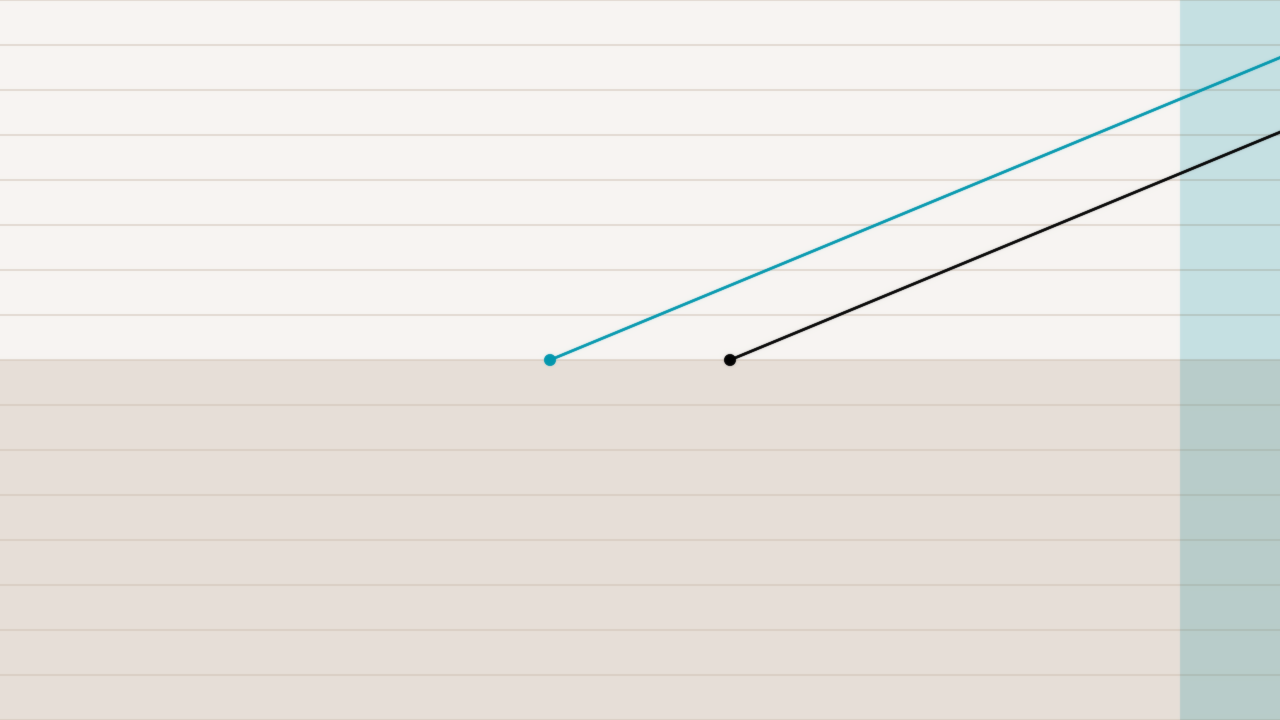
\includegraphics[width=6.5cm]{figures/rays_ge6.png}
\hspace{0.5cm}
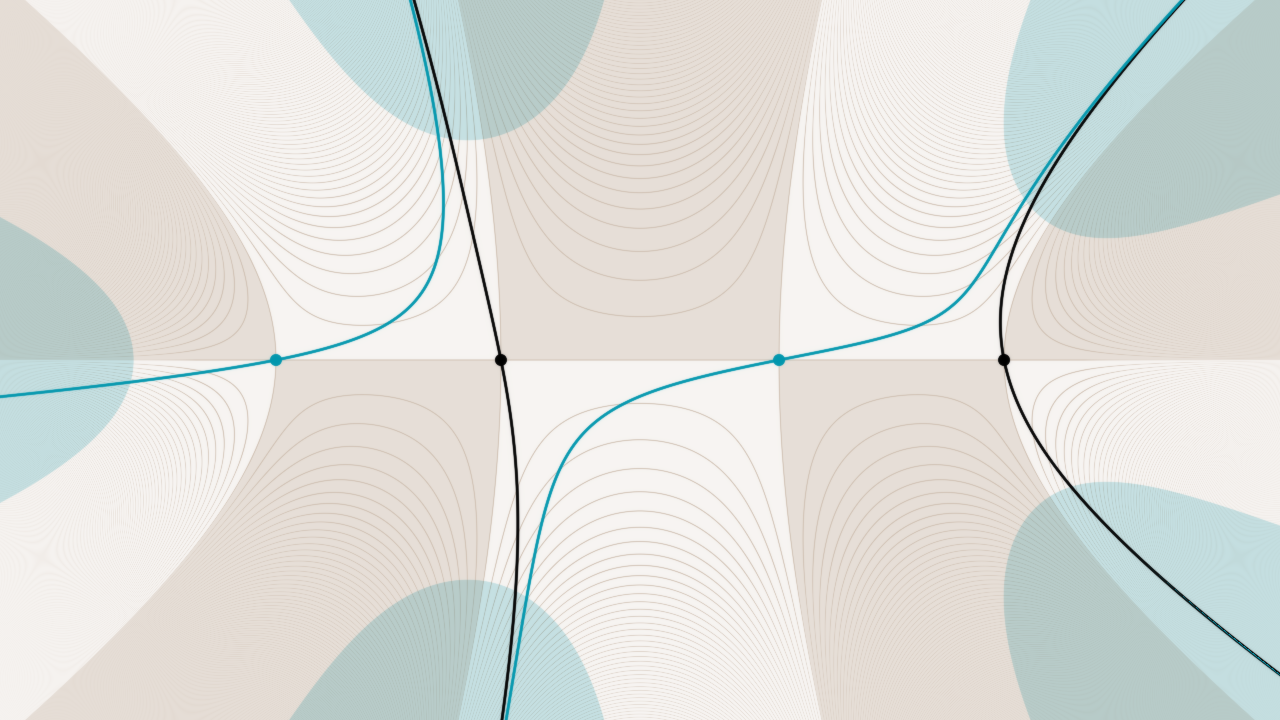
\includegraphics[width=6.5cm]{figures/thimbles-n5.png}
\captionof{figure}{On the left, we see the rays $\mathcal{J}^{\pi/8}_{\zeta, \pm 1}$ on the translation surface $B = \C$, where $\zeta$ is the standard coordinate. On the right, we see the complex manifold $X = \C$, colored according to a holomorphic map $f \maps X \to B$ whose critical values are $\zeta = \pm 1$. The Lefschetz thimbles over the rays $\mathcal{J}^{\pi/8}_{\zeta, \pm 1}$ are shown.}
\end{center}

We are now ready to define a one-dimensional thimble integral precisely, at our desired level of generality.
\begin{definition}
Fix a one-dimensional complex manifold $X$; a translation surface $B$; and a holomorphic map $f \maps X \to B$ with isolated, non-degenerate critical points. A one-dimensional {\em thimble integral} has the form
\[ I_a = \int_{\mathcal{C}_a^\theta} e^{-zf}\,\nu, \]
where $\nu$ is a holomorphic $1$-form on $X$, $a$ is a critical point of $f$, and $\mathcal{C}^\theta_a$ is the Lefschetz thimble that runs through $a$ in direction $\theta$ with a chosen orientation. Since $I_a$ depends on the frequency coordinate $z$, it is a holomorphic function on the frequency domain.
\end{definition}
We will present a proof that one-dimensional thimble integrals are always Borel regular. The proof hinges on the following well-known formula, which can be used to express any one-dimensional thimble integral as a Laplace transform.
\begin{lemma}[adapted from {\cite[Section~3.3]{pham}}]\label{lem:thimble_proj_formula}
A function $\iota_a$ with $I_a = \laplace_{\zeta, \alpha}^\theta \iota_a$ is given by the {\em thimble projection formula}
\begin{equation}\label{eqn:formula}
    \iota_a = \frac{\partial}{\partial \zeta} \left( \int_{\mathcal{C}_a^\theta(\zeta)}\nu \right),
\end{equation}
where $\mathcal{C}_a^\theta(\zeta)$ is the part of $\mathcal{C}_a^\theta$ that goes through $f^{-1}([\alpha,\zeta e^{i\theta}])$.
\end{lemma}
Notice that the path $\mathcal{C}_a^\theta(\zeta)$ used in the lemma starts and ends in $f^{-1}(\zeta)$.

Once we know $\iota_a$, we can go through the steps of the Borel regularization process and show that we end up with the same function we started with.
\begin{theorem}[also \ref{thm:maxim-proof}]\label{thm:maxim}
If the integral defining $I_a$ is absolutely convergent, then $I_a$ is Borel regular. More explicitly:
\begin{enumerate}
\item\label{part-1} The function $I_a$ has an asymptotic expansion $\series{I}_a \defeq \aexp^\theta I_a$, which lies in the space $e^{-z \alpha} z^{-1/2} \C\llbracket z^{-1}\rrbracket$. Here, $\theta$ is the direction of the ray $\mathcal{J}^\theta_{\zeta, \alpha}$ that defines the thimble.
\item\label{part-2} The Borel transform $\series{\iota}_a \defeq \borel_\zeta \series{I}_a$ converges near $\zeta = \alpha$.
\item\label{part-3} The sum of $\series{\iota}_a$ can be analytically continued along the ray $\mathcal{J}_{\zeta, \alpha}^\theta$. Its Laplace transform along that ray is well-defined, and equal to $I_a$.
\end{enumerate}
\end{theorem}
\begin{todo}[In parallel with the ODE results, does this theorem help us accomplish something interesting or justify a point of view?]\end{todo}
%
\subsubsection{Other results}\label{sec:other_results}
%
\paragraph{New perspectives on the Laplace transform}
%
For Borel summation to work as described in Theorems~\ref{thm:soln_is_Borel_sum} and~\ref{thm:maxim}, one usually needs to take the Laplace and Borel transforms using a particular position coordinate and integration base point. To explain this aspect of Borel regularity, we introduce a geometric picture of the Laplace and Borel transforms, generalizing the position domain from the complex plane to a translation surface $B$. Each translation chart $\zeta$ gives a different version of the Laplace transform, whose associated frequency domain is the cotangent space $T^*_{\zeta = 0} B$. The frequency coordinate $z$ is a canonical coordinate on $T^*_{\zeta = 0}B$, or on $T^*_{\zeta = 0}B^{\otimes n}$ if $\zeta = 0$ is a singularity with cone angle $2\pi n$. The details of this picture are discussed in Sections \ref{sec:geometry_laplace} and \ref{sec:geometry_borel}.
\begin{center}
\phaseSpaceLaplace
\captionof{figure}{The frequency coordinate $z$ on the cotangent spaces of an ordinary point and a singular point. The singularity shown here has cone angle $6\pi$, like the singularities of the translation surface associated with the Airy function.}
\end{center}

We depart slightly from traditional Laplace transform methods for solving ODEs. One traditionally relates ODEs on the frequency domain to ODEs on the position domain~\cite{braaksma2006laplace,laplace-tfm}, but we find it more natural to relate them to integral equations on the position domain. The good behavior of integral equations and their solutions is central to our proof that certain ODEs have Borel regular solutions.
%
\paragraph{New and old examples}
%
We illustrate our main results with detailed treatments of several examples. Generalizing the classic example of the Airy equation (Appendix~\ref{airy-appendix}), we find frames of Borel regular solutions for the Airy--Lucas and generalized Airy equations (Sections \ref{example_AL} and \ref{sec:gen-airy}). Noting that the Airy--Lucas equations reduce to special cases of the modified Bessel equation, we also find Borel regular solutions of the general modified Bessel equation (Section~\ref{sec:mod-bessel-lift}). Similarly, noting that the Airy function is a thimble integral with a third-degree polynomial in the exponent, we show that a general third-degree thimble integral is Borel regular (Section~\ref{sec:deg3}). Finally, as an example of a fourth-order ODE, we solve the equation describing the vibration of a triangular cantilever (Section~\ref{sec:catilever}).

Each of our examples focuses on either a level~1 ODE whose solutions can be expressed as thimble integrals or a thimble integral that satisfies a level~1 ODE. This provides an opportunity to compare different explanations for why each example function is Borel regular.

In the literature on Borel summation, the Airy equation has been discussed many times, using different approaches and conventions. In Section~\ref{airy-comparison}, we explain how the treatments in \cite[Section 2.2]{lectures-Marino}, \cite[Section 6.14]{diverg-resurg-i}, and \cite[Section 2.2]{kawai-takei} line up with ours.
 \begin{todo}Other treatments of the anharmonic oscillator: \cite{bender-wu}\cite[Appendix B]{aniceto2019primer}\cite[Section 2.5.3]{sternin1995borel}).\end{todo}
%
\paragraph{Links to resurgence}
%
The examples we study all involve {\em resurgent functions} in the position domain. \begin{todo}[Say a tiny bit about what resurgence does or is good for.]\end{todo} The theory of resurgence has been applied extensively to linear ODEs \cite{loday1994stokes,diverg-resurg--ii}, and it has yielded results about non-linear ODEs as well~\cite{costin-PI,costin_kruskal,diverg-resurg-iii,schiappa-PI}. Geometric arguments show that when a thimble integral has a holomorphic Morse function in the exponent, as we have in at least some of our examples, the corresponding function on the position domain is always resurgent~\cite{Maxim_slide_ERC}\cite[Section 6.2]{kontsevich2022analyticity}. Conjecturally, this property extends to more general thimble integrals---perhaps even infinite-dimensional ones \cite[examples~5--6]{Maxim_slide_ERC}. The linear ODEs and $1$-dimensional thimble integrals that we study provide toy examples of how resurgent functions arise and behave. \begin{revised}As a concrete example, in Section~\ref{resurgence-AL}, we use resurgence to find the Stokes constants of the Airy--Lucas equations.\end{revised}
%
\subsection{Organization of the paper}\label{sec:org}
\begin{revised}
%
\begin{paragraph}{Section~\ref{sec:historical-context}}
We contextualize our work by reviewing some classical results related to Borel regularity. These results come from the literature on asymptotics, ODEs, and integrals over Lefschetz thimbles.\end{paragraph}
%
\begin{paragraph}{Section~\ref{sec:Laplace-Borel-general}}
We introduce a geometric perspective on the Laplace and Borel transforms, which will be useful for stating and proving our results. To make this section more self-contained, we review basic definitions and properties in Section~\ref{laplace:ordinary} and the beginnings of Sections \ref{sec:geometry_borel} and \ref{sec:borel-laplace-homom}.
\end{paragraph}
%
\begin{paragraph}{Section~\ref{sec:proof_main_results}}
We restate and prove our main results.
\end{paragraph}
%
\begin{paragraph}{Section~\ref{sec:examples}}
We illustrate our results by working through detailed examples of how Borel regular functions arise, both as $1$-dimensional thimble integrals and as solutions of level~$1$ ODEs.
\end{paragraph}
%
\begin{paragraph}{Appendix~\ref{airy-appendix}}
Reprising our analysis of the Airy--Lucas equations in Section~\ref{sec:examples}, we focus on the Airy equation as a concrete special case. We then explain how our treatment lines up with other discussions of the Airy equation in the literature on Borel summation.
\end{paragraph}
%
\begin{paragraph}{Appendix~\ref{shifting}}
We prove a fact about the relationship between integral and differential equations which is used in some of our examples.
\end{paragraph}
%
\end{revised}
\begin{todo}\par [Consider going back to non-separated style.]\end{todo}\begin{draft}The paper is organized as follows: in Section~\ref{sec:historical-context} we review some well-known results concerning Borel regularity which dates back to the classical theory of asymptotics, ODEs and integrals over Lefschetz thimbles. This could help the reader to contextualize our results in the literature. Then, in Section~\ref{sec:Laplace-Borel-general} is devoted to define the new geometric picture of the Borel and Laplace transform. The reader who is not familiar with the formalism of Borel and Laplace transforms might start with Sections \ref{laplace:ordinary}, the beginning of Section~\ref{sec:geometry_borel} and of Section~\ref{sec:borel-laplace-homom}. Then, Section~\ref{sec:proof_main_results} contains proofs of the main results. Finally, in Section~\ref{sec:examples} we give a detailed treatment of different examples both from the ODE perspective and from the thimble integral one. 
We include Appendix~\ref{airy-appendix} that contains a detailed treatment of the Airy example, and it is recommended for readers less familiar to the subject. \begin{todo}[Appendix~\ref{shifting}?]\end{todo}
\end{draft}
%
\subsection{Notation}
In reasoning about Borel summation, it is important to keep track of whether we are working with holomorphic functions or formal series, and whether we are working on the position domain (the Borel plane) or the frequency domain (the $z$ plane). We have adopted a variable naming convention that makes these distinctions apparent at a glance.
\begin{notation*}
Functions and series on the frequency and position domains are named as follows.
\begin{center}
\begin{tabular}{c|c|c}
& \textbf{Analytic}: no tilde & \textbf{Formal}: tilde \\[1mm] \hline
\vphantom{\rule{0mm}{5mm}} \textbf{Frequency domain}: upper case & $\Phi$ & $\series{\Phi}$ \\[1mm] \hline
\vphantom{\rule{0mm}{5mm}} \textbf{Position domain}: lower case & $\phi$ & $\series{\phi}$ \\[1mm]
\end{tabular}
\end{center}
We will sometimes use a hat to emphasize that we got a holomorphic function $\hat{\phi}$ by taking the sum of formal series $\series{\phi}$.

The frequency and position variables $z$ and $\zeta$ are excepted from this convention. The frequency variable is lower-case, even though it lives on the frequency domain, and neither variable gets a tilde when it serves as a formal variable rather than a coordinate function.
\end{notation*}

Here are some examples of this notation in action. Since the Laplace transform $\laplace_{\zeta, 0}$ turns functions on the position domain into functions on the frequency domain, we might write $\laplace_{\zeta,0} \phi = \Phi$. On the other hand, the Borel transform $\borel_\zeta$ turns formal series in the frequency variable into formal series in the position variable, so we might write $\series{\phi} = \borel_\zeta \series{\Phi}$.
%
\subsection{Acknowledgements}
This paper is a result of the ERC-SyG project, Recursive and Exact New Quantum Theory (ReNewQuantum) which received funding from the European Research Council (ERC) under the European Union's Horizon 2020 research and innovation programme under grant agreement No 810573. 

We thank Fondation Mathematique Jacques Hadamard for supporting the visit of the second author at IH\'ES, under the program \textit{Junior Scientific Visibility}. 

We thank Fr\'{e}d\'{e}ric Fauvet, Maxim Kontsevich, Andrew Neitzke, and David Sauzin for fruitful discussions and suggestions.
%
\section{Historical context}\label{sec:historical-context}
%
\subsection{Borel regularity as a good approximation condition}
Borel regular functions can be characterized as functions that are approximated well, asymptotically, by polynomials. Watson showed a century ago \cite[Part II, Section 9]{watson2} that a function $\Phi$ is Borel regular whenever its asymptotic expansion for large $|z|$ is uniformly $1$-Gevrey-asymptotic in an obtuse-angled sector at infinity (see Definition~\ref{def:unif-gevrey-asymp}).

Watson's theorem was soon improved by Nevanlinna \cite{nevanlinna} (see a modern proof in \cite[Theorem~B.15]{nikolaev2023exact} and a generalization to power series with fractional power exponents in \cite{delabaere--rosoamanana}), and improved again later by Sokal \cite{sokal1980improvement}. These improvements tell us that the obtuse-angled sector around $\infty$ in the statement above can be replaced with an open disk whose boundary touches infinity---that is, an half-plane which does not contain $0$, and may be displaced from $0$ by some distance $\Lambda$.
\begin{center}
\begin{tikzpicture}
\setfiberscale{2.5}
\renewcommand{\phase}{35}
\newcommand{\dis}{1.2}
\begin{fiber}[shade, phase=\phase, dis=\dis]
\genfibercontent[dual]
\draw (0, 0) -- (-\phase:\rshade);
\draw[rotate=-\phase] (\dis, -0.1) -- (\dis, 0.1);
\draw (0, 0) -- (0.75, 0);
\draw[shorten <=0.3mm, shorten >=0.3mm] (0:0.5) arc (0:-\phase:0.5) node[midway, anchor=180-\phase/2] {$-\theta$};
\node[anchor=90-\phase, inner sep=2mm] at (-\phase:\dis) {$\Lambda$};
\node[anchor=north west, inner sep=2mm] at (-\rfiber, \rfiber) {$z$};
\end{fiber}
\end{tikzpicture}
\end{center}
When the half-plane extends along the $-\theta$ direction, the sum $\hat{\phi}$ of the Borel transform of $\aexp^{-\theta} \Phi$ has an absolutely convergent Laplace transform along the $\theta$ direction. In fact, we have $|\hat{\phi}| \lesssim e^{\Lambda |\zeta|}$ uniformly over a constant-radius neighborhood of the ray $\zeta \in e^{i\theta}[0, \infty)$. 
\begin{center}
\begin{tikzpicture}
\setfiberscale{2.5}
\pgfmathsetmacro{\rshade}{1.5*\rfiber}
\renewcommand{\phase}{35}
\newcommand{\radius}{0.85}
\begin{fiber}
\fill[pwbeige!30, draw=pwbeige!60, rotate=\phase] (\rshade, \radius) -- (0, \radius) arc (90:270:\radius) -- (0, -\radius) -- (\rshade, -\radius) -- cycle;
\genfibercontent
\draw (0, 0) -- (0.75, 0);
\draw[ray] (0, 0) -- (\phase:\rshade);
\draw[shorten <=0.3mm, shorten >=0.3mm] (0:0.5) arc (0:\phase:0.5) node[midway, anchor=180+\phase/2] {$\theta$};
\node[anchor=north west, inner sep=2mm] at (-\rfiber, \rfiber) {$\zeta$};
\end{fiber}
\end{tikzpicture}
\end{center}

The Watson--Nevanlinna--Sokal characterization of Borel regular functions is totally general, which means it cannot  take advantage of any extra structure provided by the problem you are trying to solve. We take the opposite approach, showing that certain functions are Borel regular just because of the extra structure provided by the problems they solve. 
%
\subsection{Solving level~$1$ ODEs}\label{sec:history_ODE}
%
The study of irregular singular differential equations on complex domains has a long history, and interesting phenoma distinguish irregular singular equations from regular singular ones. Analytic solutions of a linear ODE with an irregular singularity exhibit the Stokes phenomenon: asymptotic behavior that changes sharpy from from direction to the next. Formally, this behavior is captured in a {\em formal integral} solution: an expression
\[ \sum_{\alpha \in A} e^{-\alpha z} z^{\tau_\alpha} \series{F}_\alpha \]
in which $A$ is a finite set of complex numbers, each $\tau_\alpha$ is a real number, and each $\series{F}_\alpha$ is a formal power series in $\C\llbracket z^{-1} \rrbracket$. For each direction $\theta$, the term with the lowest value of $\Re(e^{i\theta} \alpha)$ represents the dominant contribution to the solution's asymptotic behavior.

Each term of a formal integral is an example of a {\em trans-monomial}---the basic building block of a {\em trans-series}.\footnote{For the full definition of a trans-series, see~\cite{EcalleIII,van-der-hoeven2001complex,costin_transseries,costin_summability}.} The trans-monomials in the spaces $e^{-\alpha z} z^\tau\,\C\llbracket z^{-1} \rrbracket$ are the only ones we will need to consider in this paper. Poincar\'{e}'s method for solving linear level~$1$ ODEs, discussed in Section~\ref{sec:Poincare method}, produces trans-monomial solutions in these spaces. The Poincar\'{e} solutions serve as the terms of a general formal integral. Each Poincar\'{e} solution is the asymptotic expansion of an analytic solution, whose existence is guaranteed---non-constructively---by the Main Asymptotic Existence Theorem (M.A.E.T.).

The Poincar\'{e} solutions and the M.A.E.T. have inspired several other methods for solving linear level~1 ODEs. The ones we will discuss in this section are summarized in the following table. We classify solution methods by two features: whether the solutions they produce are analytic functions or formal series, and whether they solve the original equation on the frequency domain or an equivalent equation in the position domain.
\begin{center}
\begin{tabular}{l|l|l}
& \textbf{Analytic} & \textbf{Formal} \\ \hline
\textbf{Frequency} &  & Poincar\'{e}: trans-monomial ansatz~\cite{int-irreg} \\ \hline
\textbf{Position} & \'{E}calle: resurgence  & \'{E}calle: formal perturbation theory~\cite{EcalleIII,loday-Remy2011} \\
& Fixed-point iteration~\cite{reg-sing-volterra} \\
\end{tabular}
\end{center}
%
\subsubsection{The Poincar\'{e} method and Borel summation}\label{sec:Poincare method}
%
An ODE of the form described in Section~\ref{borel-reg:explanatory-power} always has a frame of solutions in the trans-monomial spaces $e^{-\alpha z} z^{\tau_\alpha}\,\C\llbracket z^{-1} \rrbracket$. These solutions can be found systematically, using an algorithm described by Poincar\'{e}~\cite{int-irreg}\cite[Proposition~2.2.7, p.~111]{EcalleIII}. Poincar\'{e} observes \begin{verify}(Section~3)\end{verify} that when $z$ is large, the constant-coefficient equation $P\big(\tfrac{\partial}{\partial z}\big) \Phi = 0$ approximates the equation $\mathcal{P}\Phi = 0$ that we are trying to solve. The solutions of this approximate equation are the exponentials $\{e^{-\alpha z} \colon P(-\alpha) = 0\}$. Poincar\'{e} guesses that each approximate solution $e^{-\alpha z}$ can be turned into an exact solution $e^{-\alpha z} \series{F}_\alpha$ using a formal correction factor $\series{F}_\alpha \in z^{-\tau_\alpha}\,\C\llbracket z^{-1} \rrbracket$. When $\tau_\alpha = Q(-\alpha) / P'(-\alpha)$, the correction factor can be found order by order, starting from any chosen constant term. We will refer to the resulting solutions $e^{-\alpha z} \series{F}_\alpha \in e^{-\alpha z} z^{\tau_\alpha}\,\C\llbracket z^{-1} \rrbracket$ as Poincar\'{e}'s formal solutions.

Although it is not contructive, the M.A.E.T. guarantees the existence of a frame of analytic solutions asymptotic to Poincar\'{e}'s formal ones~\cite[Chapter~14]{balser}. Furthermore, the Ramis Index Theorem tells us that the Borel transform sends Poincar\'{e}'s formal solutions to convergent series on the position domain---the first step toward proving Borel summability~\cite{ramis_index}. This has motivated the development of summability methods, which promote formal solutions to analytic ones~\cite{diverg-resurg--ii,malgrange--fourier,malgrange1995sommation,malgrange92,ramis1991series}. These methods can be applied both within and beyond the world of linear level~1 ODEs.
%
\subsubsection{\'{E}calle's theory of resurgence}
%
\'{E}calle's theory of resurgence introduced a new perspective on formal solutions, mostly focused on the analysis of the position domain~\cite{EcalleIII,loday-Remy2011}. In a nutshell, resurgence provides information about the analytic continuation of the Borel transform of a divergent series. In particular, it reveals the locations of singularities in the position domain, and it quantifies the Stokes phenomenon in terms of ``Stokes constants'' describing analytic continuation around the singularities.

A series is resurgent if its Borel transform converges to an endlessly analytically continuable function on the position domain. Thus, resurgence creates a bridge between formal and analytic solutions of problems in the position domain.

The formal solutions of a level~$1$ ODE are always resurgent series~\cite[Proposition~2.2.1]{EcalleIII}. \'{E}calle proved this by using formal perturbation theory to solve a corresponding integral equation in the position domain. Using the ``formalism of singularities'' to understand how the singularities of the perturbative solution would propagate from one order of perturbation to the next, \'{E}calle showed that the pertrubation series would converge to an endlessly analytically continuable function. Loday-Richaud and Remy went on to show that this function always has a well-defined Laplace transform, so the corresponding formal solution in the frequency domain is Borel summable~\cite{loday-Remy2011}. Malgrange got similar results by working with differential equations, rather than integral equations, on the position domain~\cite{malgrange--fourier}.
%
\subsubsection{Solving Riemann--Hilbert problems}
%
\begin{revised}A level~$1$ ODE can be seen as the coordinate expression of a meromorphic connection on a principal bundle---specifically, the kind of meromorphic connection called an {\em oper}~\cite{BD-opers}. Local solutions of the ODE correspond to local flat sections of the connection. We can therefore use the theory of meromorphic connections to study level~$1$ ODEs. In particular, given an ODE, we can set up a Riemann--Hilbert problem whose solution would encode a frame of analytic solutions of the ODE. \begin{todo}[Add reference]\end{todo}

To formulate the Riemann--Hilbert problem, we fix the asymptotic behvaiour of the frame of solutions at $z = 0$ and $z = \infty$, and we also fix its discontinuities---the Stokes data prescribing how the frame jumps across each Stokes ray. A solution is then given by a piecewise analytic function which is holomorphic away from the Stokes rays and has the prescirbed asymptotics and discontinuities.\end{revised}

In many cases, the solutions of Riemann--Hilbert problems can be found explicitly~\cite{Dubrovin-tt_star,Dubrovin-Heun,GMN1,Tom-RH-1,Tom-RH-conifold,BBS-RH}. These cases include some Riemann--Hilbert problems arising from level~1 ODEs. For example, in Section~6.2.1 of \cite{kontsevich2022analyticity}, Kontsevich and Soibelman discuss a Riemann--Hilbert problem for thimble integrals using the formalism of analytic wall-crossing structures. As mentioned in Section~\ref{borel-reg:explanatory-power}, every thimble integral satisfies some ODE. Kontsevich and Soibelman also explain why the asymptotics of these thimble integrals are resurgent series.
\begin{todo}\par
Discuss examples where the Riemann--Hilbert problem corresponding to an ODE can be solved.
\begin{itemize}
\item Dubrovin
\item Kontsevich--Soibelman
\item Bridgeland
\item Gaiotto--Moore--Nietzke
\end{itemize}
\end{todo}
%
\subsubsection{Laplace transform methods and fixed point iteration}
%
All of the historical approaches we have discussed so far start by looking for formal solutions. In this paper, we will focus on a different kind of approach, where we start by looking for analytic solutions expressed as Laplace transforms. By carefully choosing the starting point of the Laplace transform, we get analytic solutions which are asymptotic to Poincar\'{e}'s formal ones. These solutions will turn out to be Borel regular.

We use the Laplace transform to turn differential equations on the frequency domain into integral equations on the position domain. This runs parallel to \'{E}calle's use of the Borel transform. Building on the existence and uniqueness results we proved in~\cite{reg-sing-volterra}, we use Picard iteration to solve the integral equation in the position domain, and to show that the corresponding solution in the frequency domain is Borel regularizable.

The function spaces mentioned in Section~\ref{sec:laplace_analytic} play an important role in our approach. They also appear in the work of Braaksma, who uses them to solve systems of ODEs whose coefficients are expressed as Laplace transforms~\cite{braaksma2006laplace}. This overlap suggests an opportunity to combine the two approaches, extending our results to systems of equations, and Braaksma's to equations with more general coefficients.
%
\subsection{Thimble integrals}
%
Thimble integrals have been studied from different perspectives: in physics, they play an important technical role in quantum mechanics, where infinite-dimensional exponential integrals are supposed to give the expectation values of observable quantities \cite{dunne-unsal2,dunne-unsal,Fauvet_Menous_Queva,Tanizaki:2014tua}. In the algebraic geometric set-up, namely when, following the notation introduced in Section~\ref{borel-reg:explanatory-power}, $X$ is an $N$-dimensional alegbraic variety over $\C$ and $f$ is a proper map $f\colon X\to\C$, thimble integrals are known as period integrals \cite{deligne2007singularites,Maxim_lectures,pham}.\footnote{In particular, they find application in mirror symmetry for Fano varieties as they encode the Gromov--Witten invariants. \begin{todo}[\textbf{V} Add references---Maxim's mirror symmetry talk, Varchenko.]\end{todo}}
\subsubsection{Thimble integrals in physics}
In wave optics, a thimble integral can arise when we adds up the secondary waves emanating from all the points along a wavefront~\cite{Fenyes-ihes-lecture}. For example, the Airy integral approximates the sum of the secondary waves coming from a wavefront with an inflection point~\begin{todo}[``the mathematical physics of rainbows and glories'']\end{todo}. \begin{todo}The formalism of wave optics can also be applied to the scattering of quantum particles---for example, in the ``nuclear optical model'' [Knoll--Schaeffer]. [This inspired Voros's work in ``The return of the quartic oscillator'']\end{todo} In the path integral picture of quantum mechanics, which draws inspiration from wave optics, infinite-dimensional thimble integrals are supposed to give the expectation values of observable quantities. In this context, the integral's formal asymptotic expansion is often better-defined than the integral itself, so physicists use Borel summation, resurgence, and related techniques to assign the integral a value. For instance, in the two-dimensional, $\mathcal{N}=2$ supersymmetric QFTs given by Landau--Ginzburg theories, Cecotti and Vafa showed that instantons can be computed using Picard--Lefschetz formulas. Indeed, the so called wall-crossing phenomenon is equivalent to Stokes phenomenon for thimble integrals~\cite{Cecotti:1992rm}. Similarly, in complex Chern--Simons theory, the path integral can be studied by decomposing it into thimble integrals and then arguing as in finite dimesion~\cite{gukov-marino-purtrov-resurgence,Witten}. Other examples can be found in~\cite{costin_kruskal,Garoufalidis--CS,GTM--CS,GGM,dunne-unsal2,dunne-unsal,Fauvet_Menous_Queva,Tanizaki:2014tua,Berry_Howls,Berry1991,Howls97,Howls,pham1988resurgence,Unsal--resurgence-gauge}. \begin{todo}[\textbf{V} Is it true that all thimble integrals describes instantions? Can we have (higher dimensional) thimble integrals describing renormalons?]\end{todo}
%
\subsubsection{Thimble integrals in geometry}
Thimble integrals can be used to explore the geometry of complex manifolds, and even to represent elements of a homology group. To see how this works, we first recall how the one-dimensional definition of a Lefschetz thimble arises from the general definition. Suppose that $f \maps X \to B$ is a holomorphic map from an $N$-dimensional complex manifold $X$ to a translation surface $B$. Consider a translation chart $\zeta$ on $B$ and a non-degenerate critical point $a \in X$ that $f$ sends to $\zeta = \alpha$. Near $a$, we can always find coordinates $t_1, \ldots, t_N$ on $X$ with
\[ f^*\zeta = \alpha + e^{i \theta} (t_1^2 + \ldots + t_N^2). \]
When the ray $\mathcal{J}_{\zeta, \alpha}^\theta$ avoids the other critical values of $f$, each such coordinate system defines a Lefschetz thimble: the oriented real-analytic submanifold where $t_1, \ldots, t_N$ are real. There are many such coordinate systems, but they are all related by local holomorphic maps from $X$ to the complex orthogonal group $O_N(\C)$. Since $O_N(\C)$ has only two connected components, distinguished by the sign of the determinant, a Lefschetz thimble is determined up to homotopy and orientation by the critical point $a$ and the direction $\theta$. When $N = 1$, the homotopy freedom disappears, because $O_1(\C)$ is the discrete group $\{\pm 1\}$.

Lefschetz thimbles for $f$ with direction $\theta$ represent classes in the ``rapid decay homology'' group $H^\theta_N(X,f)$~\cite{pham}\cite[Section~1.1]{fresan-notes}. Roughly speaking, this group describes homology relative to the region where $\Re(e^{-i\theta} f)$ is large and positive. In this context, each thimble integral
\[ \int_{\mathcal{C}}e^{-zf}\,\nu \]
computes the pairing between a rapid decay homology class $\mathcal{C}$ and a ``twisted $1$-form'' $e^{-zf}\,\nu$. When all the critical points of $f$ are non-degenerate, Lefschetz thimbles actually form a basis for $H^\theta_N(X,f)$. As $\theta$ varies, the groups $H^\theta_N(X,f)$ fit together into a local system over the circle of directions, which is singular at the direction of each segment connecting a pair of critical values. The monodromy of this local system can be found using the Picard--Lefschetz formula~\cite[Section~1]{Arnold}\cite[Section~3.3, Part II]{pham}.

Like solutions of level~$1$ ODEs, thimble integrals often exhibit the Stokes phenomenon. For one dimensional thimble integrals, the Stokes constants can be interpreted geometrically as intersection numbers for pairs of thimbles~\cite{kontsevich2022analyticity}. More generally, finding the Stokes constants is equivalent to finding the monodromy of the local system $H^\theta_N(X,f)$ (see the recent developement~\cite{kontsevich2024holomorphic}).
%
\subsubsection{Asymptotics of thimble integrals}
%
Thimble integrals are traditionally understood through their asymptotics, which can be found with the saddle point approximation~\cite{andersen2020resurgence,delabaere-howls,delabaere_dillinger_pham,Delabaere-Pham99,dingle1973asymptotic,Malgrange22,Pham83}. The asymptotic expansion of a thimble integral is typically divergent, but its Borel sum often matches the integral it came from. In other words, thimble integrals tend to be Borel regular. Theorem~\ref{thm:maxim} explains why this happens in the one-dimensional case.

To prove Theorem~\ref{thm:maxim}, we first shift our focus from the thimble integral to the corresponding analytic object in the position domain. The integral contains a hint about where to find this analytic object: the thimble itself, which is a real-analytic submanifold of a complex manifold. When the thimble is one-dimensional, we can use the well-known formula in Lemma~\ref{lem:thimble_proj_formula} to turn it into a function whose Laplce transform is the thimble integral. This formula generalizes to higher-dimensional thimbles~\cite{pham} and thimbles based at degenerate critical points~\cite[Section 1.2.2]{mistegard_phdthesis}.
%
\section{The Laplace and Borel transforms}\label{sec:Laplace-Borel-general}
\subsection{The geometry of the Laplace transform}\label{sec:geometry_laplace}
Classically, the Laplace transform turns functions on the position domain into functions on the frequency domain. In the study of Borel summation and resurgence, it is useful to see the position domain as a {\em translation surface} $B$, and the frequency domain as one of its cotangent spaces. Roughly speaking, the Laplace transform lifts holomorphic functions on $B$ to holomorphic functions on $T^*B$.
%
\subsubsection{Background on translation surfaces}\label{sec:transl}
%
\paragraph{A brief definition}
%
A translation surface is a Riemann surface $B$ carrying a holomorphic $1$-form $\lambda$~\cite{zorich2006flat}. A {\em translation chart} is a local coordinate $\zeta$ with $d\zeta = \lambda$. The standard metric on $\C$ pulls back along translation charts to a flat metric on $B$, with a conical singularity of angle $2\pi n$ wherever $\lambda$ has a zero of order $n-1 > 0$.

We will call the zeros of $\lambda$ {\em branch points}. To explore the region around a branch point, it can be helpful to use a {\em translation parameter}: a function $\zeta$ which has $d\zeta = \lambda$, but is not necessarily a local coordinate.

In all of our examples, $B$ will be a finite-type Riemann surface, and $\lambda$ will have a pole at each puncture. This level of generality allows for plenty of interesting behavior without letting $B$ get too messy. Sections~2.4\;--\;2.5 of \cite{gupta2013meromorphic} give a sense of what $B$ can look like near a pole of $\lambda$.
%
\paragraph{A sense of direction}
%
The translation structure gives $B$ a notion of direction as well as distance. Away from the branch points, we can talk about moving upward, rightward, or at any angle, just as we would on $\C$. At a branch point of cone angle $2\pi n$, we can also talk about moving upward, rightward, or at any angle in $\R/2\pi\Z$, but here there are $n$ directions that fit each description. To make this more concrete, note that around any point $b \in B$, there is a unique translation parameter $\zeta_b$ that vanishes at $b$. This parameter is a translation chart when $b$ is an ordinary point, and an $n$-fold branched covering of $\C$ when $b$ is a branch point of cone angle $2\pi n$. In either case, $\zeta_b \in e^{i\theta} [0, \infty)$ is a ray or a set of rays leaving $b$ at angle $\theta \in \R/2\pi\Z$.

Near each branch point $b$, fix a coordinate $\omega_b$ with $\zeta_b = \tfrac{1}{n} \omega_b^n$, where $2\pi n$ is the cone angle at $b$. This lets us label each direction at $b$ with an ``extended angle'' in $\R/2\pi n\Z$. Of course, there are $n$ different choices for $\omega_b$.
%
\paragraph{The frequency coordinate}\label{transl-freq}
%
Over the complement $B'$ of the branch points, the translation structure gives us a holomorphic map $z \maps T^*B' \to \C$. This map is an isomorphism on every fiber, trivializing $T^*B$ almost globally. Over a branch point $b$ of cone angle $2\pi n$, we get an analogous isomorphism $z \maps T^*_bB^{\otimes n} \to \C$. In both cases, we will call $z$ the {\em frequency coordinate} of $B$.
\begin{center}
\phaseSpaceLaplace
\captionof{figure}{The frequency coordinate $z$ on the cotangent spaces of an ordinary point and a singular point. The singularity shown here has cone angle $6\pi$, like the singularities of the translation surface associated with the Airy function.}
\end{center}

At an ordinary point, we can define $z$ simply as the map
\begin{align*}
z \maps T^*_bB & \to \C \\
\lambda\big|_b & \mapsto 1.
\end{align*}
To generalize $z$ to branch points, though, we need a more sophisticated definition. Recall that $T^*_bB = \van_b / \van_b^2$, where $\van_b$ is the ideal of holomorphic functions that vanish at $b$. Observing that $(f + \van_b)^n$ lies within $f^n + \van_b^{n+1}$ for any $f \in \van_b$, we can identify $T^*_bB^{\otimes n}$ with $\van_b^n / \van_b^{n+1}$ for $n \ge 1$. When $b$ is an ordinary point, the translation parameter $\zeta_b$ that vanishes at $b$ represents a nonzero element of $\van_b / \van_b^2$: the cotangent vector $\lambda\big|_b$. In general, $\zeta_b$ represents a nonzero element of $\van_b^n / \van_b^{n+1}$, where $2\pi n$ is the cone angle at $b$. We define $z$ as the isomorphism
\begin{align*}
z \maps \van_b^n / \van_b^{n+1} & \to \C \\
\zeta_b + \van^{n+1} & \mapsto 1.
\end{align*}
When $b$ is a branch point, the coordinate $\omega_b$ we fixed in ``A sense of direction'' gives us an isomorphism
\begin{align*}
w_b \maps T^*_bB & \to \C \\
\omega_b + \van^2 & \mapsto 1
\end{align*}
that makes the diagram
\begin{center}
\begin{tikzcd}
T^*_bB^{\otimes n} \arrow[r,"z"] & \C \\
T^*_bB \arrow[u,"\blankbox^n"] \arrow[r,"w"'] & \C \arrow[u,"\blankbox^n"']
\end{tikzcd}
\end{center}
commute. Here, $\blankbox^n$ represents the $n$th-power map.
%
\subsubsection{The Laplace transform over an ordinary point}\label{laplace:ordinary}
%
Pick a translation parameter $\zeta$ on $B$ and an extended angle $\theta \in \R$. The {\em Laplace transform} $\laplace_{\zeta, \alpha}^\theta$ turns a local holomorphic function $\phi$ on $B$ into a local holomorphic function on $T^*_{\zeta = 0} B$. When $\zeta = 0$ is an ordinary point, the Laplace transform is defined by the formula
\begin{equation}\label{laplace:int}
\laplace_{\zeta, \alpha}^\theta \phi = \int_{\mathcal{J}_{\zeta, \alpha}^\theta} e^{-z\zeta} \phi\,d\zeta,
\end{equation}
where $z$ is the frequency function and $\mathcal{J}_{\zeta, \alpha}^\theta$ is the ray $\zeta \in \alpha + e^{i\theta} [0, \infty)$. To make sense of this formula, we ask for the following conditions.
\begin{itemize}
\item The starting point $\zeta = \alpha$ is in the domain of $\zeta$. Once we have this, we can continue $\zeta$ along the whole ray $\mathcal{J}_{\zeta, \alpha}^\theta$.
\item The ray $\mathcal{J}_{\zeta, \alpha}^\theta$ avoids the branch points after leaving $\zeta = \alpha$.
\item The integral converges. We ensure this by putting conditions on $\phi$ and $z$.
\begin{itemize}
\item With respect to the flat metric, $\phi$ is uniformly of exponential type $\Lambda$ along the ray $\mathcal{J}_{\zeta, \alpha}^\theta$, and is locally integrable throughout the ray.\footnote{Recall that a function $\phi$ is of exponential type $\Lambda$ if for every $\varepsilon>0$, there is a constant $A_\varepsilon$ (which may depends on $\varepsilon$) such that $|\phi|\le A_\varepsilon e^{(\Lambda+\varepsilon)|\zeta|}$. We instead require a uniform constant $A$ such that $|\phi| \le A e^{\Lambda|\zeta|}$.}
\item The value of $z$ satisfies the inequality $\Re(e^{i\theta} z) > \Lambda$, which cuts out a half-plane $H^\theta_\Lambda$ in $T^*_{\zeta = 0} B$.
\end{itemize}
\end{itemize}
For any $\sigma > -1$, the conditions on $\phi$ are satisfied by all of the functions in the spaces $\singexp{\sigma}{\Lambda}(\Omega_\alpha)$ introduced in \cite{reg-sing-volterra}. Here, the domain $\Omega_\alpha$ must contain the ray $\mathcal{J}_{\zeta, \alpha}^\theta$, and the norm $\|\cdot\|_{\sigma, \Lambda}$ is taken with respect to $\zeta = \alpha$.
\subsubsection{The Laplace transform over a branch point}
When $\zeta = 0$ is a branch point, we can still use formula~\eqref{laplace:int} to define $\laplace_{\zeta, \alpha}^\theta \phi$ on $T_{\zeta = 0}^*B$, as long as we take care of a few subtleties. Thanks to the labeling choices we made in Section~\ref{sec:transl}, the extended angle $\theta \in \R$ still picks out a ray $\mathcal{J}_{\zeta, \alpha}^\theta$. The function $z$ is defined on $T_b^*B^{\otimes n}$, where $2\pi n$ is cone angle at $\zeta = 0$, so we pull it back to $T^*_{\zeta = 0} B$ along the $n$th-power map. This amounts to substituting $w_b^n$ for $z$ in formula~\eqref{laplace:int}. The inequality $\Re(e^{i\theta} z) > \Lambda$ cuts out a half-plane in $T_b^*B^{\otimes n}$, which pulls back to $n$ sector-like regions in $T_b^*B$ of angle $\pi/n$. We only define $\laplace_{\zeta, \alpha}^\theta \phi$ on one of them: the one centered around the ray $w_b \in e^{-i\theta/n}[0, \infty)$.
\subsubsection{Change of translation chart}\label{sec:change-translation}
\begin{todo}[Change $b$ to $\alpha$? \textit{V} Did it \textbf{A} Double-check]\end{todo} Suppose $\zeta$ is a translation chart on $B$, and $\zeta = \alpha$ is an ordinary point. Let $\zeta_\alpha$ be the translation chart with $\zeta = \alpha + \zeta_\alpha$. The Laplace transforms $\laplace_{\zeta_\alpha, 0}$ and $\laplace_{\zeta, \alpha}$, which both turn functions on $B$ into functions on $T^*_{\zeta = \alpha}B$, are related in the following way.
\begin{lemma}\label{translation}
If the Laplace transform of $\varphi$ is well-defined, then
   \begin{equation}
    \label{change-chart}
    e^{-z\alpha} \laplace_{\zeta_\alpha, 0} \varphi = \laplace_{\zeta, \alpha} \varphi.
\end{equation}
\end{lemma}
\begin{proof}
With a change of variable in the integral that defines the Laplace transform, we see that
\begin{align*}
\laplace_{\zeta, \alpha} \varphi & = \int_{\mathcal{J}_{\zeta,\alpha}} e^{-z \zeta}\,\varphi\;d\zeta \\
& = \int_{\mathcal{J}_{\zeta_\alpha,0}} e^{-z(\alpha + \zeta_\alpha)}\,\varphi\;d\zeta_\alpha \\
& = e^{-z\alpha } \int_{\mathcal{J}_{\zeta_\alpha,0}} e^{-z\zeta_\alpha}\,\varphi\;d\zeta_\alpha \\
& = e^{-z\alpha } \laplace_{\zeta_\alpha, 0} \varphi.
\end{align*}
\end{proof}
We now consider a rescale of the translation structure of $B$, expanding displacements by a factor of $\mu \in (0, \infty)$. The coordinate $\xi = \mu\zeta$ is a chart for the new translation structure. The corresponding frequency coordinate $x \maps T^*B \to B$ is given by $d\xi \mapsto 1$, so $x = \mu^{-1} z$. 
\begin{lemma}
Let $\varphi\in\singexp{\sigma}{\Lambda}(\Omega)$ with $\sigma>-1$ and for some $\Lambda>0$, then
    \[ \laplace_{\xi, 0} \varphi = \mu\,\laplace_{\zeta, 0} \varphi. \]
\end{lemma}
\begin{proof}
    From the computation 
    \begin{align*}
\laplace_{\xi, 0} \varphi & = \int_{\mathcal{J}_{\xi, 0}} e^{-x\xi}\,\varphi\;d\xi \\
& = \int_{\mathcal{J}_{\zeta, 0}} e^{-z \zeta}\,\varphi\;\mu\,d\zeta \\
& = \mu\,\laplace_{\zeta, 0} \varphi
\end{align*}
we get the desired result. 
\end{proof}
%
%Note that $\laplace_{\xi, 0}$ is defined in the new translation structure on $B$, while $\laplace_{\zeta, 0}$ is defined in the old translation structure. We can still compare them because they both turn complex-valued functions on $B$ into holomorphic functions on $T^*B$.
\subsection{Analysis of the Laplace transform}\label{sec:laplace_analytic}
%
\subsubsection{Regularity and decay properties}\label{sec:reg-decay}
%
%% \textcolor{orange}{[Revise]} Let $\Omega_\beta \subset B$ be an open, simply connected set that touches but does not contain $\zeta = \beta$, as shown \textcolor{RoyalBlue}{(see Figure \ref{Fig:domain})}. Suppose $\Omega_\beta$ contains the ray $\mathcal{J}_{\zeta, \beta}^\theta$. In \cite{reg-sing-volterra} we introduce the function space $\singexp{\sigma}{\Lambda}(\Omega_\beta)$ of holomorphic functions on $\Omega_\beta$ which are uniformly of exponential type $\Lambda$ and blow up like $|\zeta - \beta|^\sigma$ as $\zeta$ approaches $\beta$. When $\sigma>-1$, the singularity at $\zeta = \beta$ is integrable. Hence, the Laplace transform $\laplace_{\zeta, \beta}^\theta$ turns elements of $\singexp{\sigma}{\Lambda}(\Omega_\beta)$ into well-defined holomorphic functions on the half-plane $\Re(e^{i\theta} z) > \Lambda$ in the cotangent space $T_{\zeta = \beta}^*B$~\cite[Section  5.6]{diverg-resurg-i}.
%%
Suppose $\Omega_\alpha$ is an open sector with $\zeta = \alpha$ at its tip, and an opening angle of $\pi$ or less. For any $\Lambda \in \R$, let $\widehat{\Omega}_\alpha^\Lambda$ be the union of the half-planes $\Re(e^{i\theta} z) > \Lambda$ over all angles $\theta$ in the opening of $\Omega_\alpha$.
\begin{center}
\begin{tikzpicture}
\setfiberscale{2}
\pgfmathsetmacro{\rshade}{1.5*\rfiber}
\newcommand{\dis}{1}
\renewcommand{\phase}{0}
\newcommand{\spread}{30}

\begin{fiber}
\fill[pwbeige!30, draw=pwbeige!60] (0, 0) -- (\phase-\spread:1.5*\rshade) -- (\phase+\spread:1.5*\rshade) -- cycle;
\genfibercontent
\node[anchor=-11, inner sep=2mm] at (0,0) {$\zeta = \alpha$};
\node[anchor=north west, inner sep=2mm] at (-\rfiber, \rfiber) {$\zeta$};
\end{fiber}

\begin{scope}[shift={(5.5, 0)}]
\begin{fiber}
\fill[pwbeige!30, draw=pwbeige!60] (-\phase-\spread:\dis) +(-\phase-\spread-90:\rshade) -- +(0, 0) arc (-\phase-\spread:-\phase+\spread:\dis) -- ++(-\phase+\spread+90:\rshade) -- (\rshade, \rshade) -- (\rshade, -\rshade) -- (0, -\rshade) -- cycle;
\genfibercontent[dual]
%%\node[anchor=90-\phase, inner sep=2mm] at (-\phase:\dis) {$\Lambda$};
\node[anchor=north west, inner sep=2mm] at (-\rfiber, \rfiber) {$z$};
\end{fiber}
\end{scope}
\end{tikzpicture}
\captionof{figure}{A sector $\Omega_\alpha$ in the position domain, and the corresponding union of half-planes $\widehat{\Omega}_\alpha^\Lambda$ in the frequency domain.}\label{fig:sectorial_domain-pos-fre}
\end{center}
Let $\dualsingexp{\sigma}(\widehat{\Omega}_\alpha^\Lambda)$ be the space of holomorphic functions $\Phi$ on $\widehat{\Omega}_\alpha^\Lambda$ with $|\Phi| \lesssim \Delta^\sigma$, where $\Delta$ is the function that measures distance to the boundary of $\widehat{\Omega}_\alpha^\Lambda$. The norm $\|\Phi\|_{\sigma, \Lambda} = \sup_{\widehat{\Omega}_\alpha^\Lambda} \Delta^{-\sigma} |\Phi|$ turns $\dualsingexp{\sigma}(\widehat{\Omega}_\alpha^\Lambda)$ into a Banach space.

We will often make statements about $\dualsingexp{\sigma}(\widehat{\Omega}_\alpha^\Lambda)$ that hold when $\Lambda$ is large enough. Since restriction gives an inclusion $\dualsingexp{\sigma}(\widehat{\Omega}_\alpha^\Lambda) \hookrightarrow \dualsingexp{\sigma}(\widehat{\Omega}_\alpha^{\Lambda'})$ whenever $\Lambda < \Lambda'$, we can define a colimit space $\dualsingexp{\sigma}(\widehat{\Omega}_\alpha^\bullet)$ that all of the spaces $\dualsingexp{\sigma}(\widehat{\Omega}_\alpha^\Lambda)$ include into. \begin{todo}[\textbf{A} improve definition; \textbf{V} is this definition descriptive enough?]\end{todo}
\begin{todo}\par
[Cite \cite{sternin1995borel} better for the theorem. Note that these results don't depend on which cotangent fiber we're mapping into. $\widehat{\Omega}$ is defined across all cotangent fibers over ordinary points.]
\end{todo}
%
\begin{prop}[following~\cite{sternin1995borel}]\label{prop:laplace-cont}
Let $\Omega_\alpha$ be an open sector with $\zeta = \alpha$ at its tip, and an opening angle of $\pi$ or less. For any $\sigma > 0$ and $\Lambda \ge 0$, and any angle $\theta$ in the opening of $\Omega_\alpha$, the Laplace transform $\laplace_{\zeta_\alpha, 0}^\theta$ is a continuous map $\singexp{\sigma-1}{\Lambda}(\Omega_\alpha) \to \dualsingexp{-\sigma}(\widehat{\Omega}_\alpha^\Lambda)$, with a norm of at most $\Gamma(\sigma)$.
\end{prop}
\begin{proof}
Given some $\phi \in \singexp{\sigma-1}{\Lambda}(\Omega_\alpha)$, we compute
\begin{align*}
|\laplace_{\zeta_\alpha, 0}^\theta \phi| & = \left| \int_{\mathcal{J}_{\zeta_\alpha, 0}^\theta} e^{-z\zeta_\alpha} \phi\,d\zeta_\alpha \right| \\
& \le \int_{\mathcal{J}_{\zeta_\alpha,0}^\theta} e^{-\Re(z\zeta_\alpha)} |\zeta_\alpha|^{\sigma-1} e^{\Lambda |\zeta_\alpha|} \|\phi\|_{\sigma-1, \Lambda}\,|d\zeta_\alpha| \\
& \le \int_{\mathcal{J}_{\zeta_\alpha,0}^\theta} e^{(\Lambda - c_{z, \theta}|z|)|\zeta_\alpha|} |\zeta_\alpha|^{\sigma-1} \|\phi\|_{\sigma-1, \Lambda}\,|d\zeta_\alpha|,
\end{align*}
where $c_{z, \theta}$ is the cosine of $\arg(z) + \theta$. When $|z|$ is large and $c_{z, \theta}$ is positive, the integrand shrinks exponentially as $|\zeta|$ grows. This shows that for each angle $\theta$ in the opening of $\Omega_\alpha$, the integral defining $\laplace_{\zeta_\alpha, 0}^\theta \phi$ converges in some region of $\widehat{\Omega}_\alpha^\Lambda$. It also shows that for different angles $\theta$, the functions $\laplace_{\zeta_\alpha, 0}^\theta \phi$ match where their domains overlap. We can therefore glue these functions together into one big Laplace transform of $\phi$, defined at large values of $|z|$ across the whole opening angle of $\widehat{\Omega}_\alpha^\Lambda$.

We can now simplify the calculation of $\laplace_{\zeta_\alpha, 0}^\theta \phi$ by looking at $\arg(z)$ and using the closest angle $\theta$ in the opening of $\Omega_\alpha$. This keeps $\Lambda - c_{z, \theta}|z|$ equal to $\Delta$, the distance to the boundary of $\widehat{\Omega}_\alpha^\Lambda$. It follows that
\begin{align*}
|\laplace_{\zeta_\alpha, 0}^\theta \phi| & \le \int_{\mathcal{J}_{\zeta_\alpha, 0}^{\arg(z)}} e^{-\Delta|\zeta_\alpha|} |\zeta_\alpha|^{\sigma-1} \|\phi\|_{\sigma-1, \Lambda}\,|d\zeta_\alpha| \\
& = \int_0^\infty e^{-\Delta t} t^{\sigma-1} \|\phi\|_{\sigma-1, \Lambda}\,dt.
\end{align*}
The integral on the last line converges throughout $\widehat{\Omega}_\alpha^\Lambda$. We can evaluate it by observing that it is a Laplace transform integral, with the roles of position and frequency played by $t$ and $\Delta$ respectively:
\[ |\laplace_{\zeta_\alpha, 0}^\theta \phi| \le \Gamma(\sigma) \Delta^{-\sigma} \|\phi\|_{\sigma-1, \Lambda}. \]
In terms of the metric on $\dualsingexp{-\sigma}(\widehat{\Omega}_\alpha^\Lambda)$ defined above, this bound says that
\[ \|\laplace_{\zeta_\alpha, 0}^\theta \phi\|_{-\sigma, \Lambda} \le \Gamma(\sigma) \|\phi\|_{\sigma-1, \Lambda}, \]
which is what we wanted to show.
\end{proof}
\begin{prop}\label{prop:inverse_laplace_analytic}
Let $\Omega_\alpha$ be an open sector of the kind described in Proposition~\ref{prop:laplace-cont}, and let $\Omega_\alpha^\varepsilon \subset \Omega_\alpha$ be the open sector created by cutting a sector of angle $\varepsilon > 0$ off each edge of $\Omega_\alpha$. Choose any $\Lambda' > \Lambda$. Under the conditions of Proposition~\ref{prop:laplace-cont}, the Laplace transform
\[ \laplace_{\zeta_\alpha, 0}^\theta \maps \singexp{\sigma-1}{\Lambda}(\Omega_\alpha) \to \dualsingexp{-\sigma}(\widehat{\Omega}_\alpha^\Lambda) \]
has a continuous left inverse
\[ \left(\laplace_{\zeta_\alpha, 0}^\theta\right)^{-1} \maps \dualsingexp{-\sigma}(\widehat{\Omega}_\alpha^\Lambda) \to \singexp{\sigma-1}{\Lambda'}(\Omega_\alpha^\varepsilon), \]
with a norm of at most
\[ \frac{\Gamma(1-\sigma)}{\pi\,\sin(\varepsilon/2)}. \]
\end{prop}
\begin{proof}
Define the sector $\Omega_\alpha^{\varepsilon/2} \subset \Omega_\alpha$ similarly to $\Omega_\alpha^\varepsilon$. Choosing some $\Lambda' > \Lambda$, let $\widehat{\Omega}_\alpha^{\varepsilon/2, \Lambda'} \subset \widehat{\Omega}_\alpha^\Lambda$ be the union of the half-planes $\Re(e^{i\theta} z) > \Lambda'$ over all angles $\theta$ in the opening of $\Omega_\alpha^{\varepsilon/2}$. 
%
The boundary of $\widehat{\Omega}_\alpha^{\varepsilon/2, \Lambda'}$ forms a path $\mathcal{C}$, which we orient so that the boundary of $\widehat{\Omega}_\alpha^\Lambda$ is on its left.
\begin{center}
\begin{tikzpicture}
\setfiberscale{2.5}
\pgfmathsetmacro{\rshade}{1.5*\rfiber}
\newcommand{\dis}{1.25}
\renewcommand{\phase}{0}
\newcommand{\spread}{30}

\newcommand{\pathdis}{1.5625}
\newcommand{\pathspread}{20}

\begin{fiber}
% the region
\fill[pwbeige!30, draw=pwbeige!60] (-\phase-\spread:\dis) +(-\phase-\spread-90:\rshade) -- +(0, 0) arc (-\phase-\spread:-\phase+\spread:\dis) -- ++(-\phase+\spread+90:\rshade) -- (\rshade, \rshade) -- (\rshade, -\rshade) -- (0, -\rshade) -- cycle;

% grid lines and stuff
\genfibercontent[dual]

% the path
\draw[very thick] (-\phase-\pathspread:\pathdis) +(-\phase-\pathspread-90:\rshade) -- +(0, 0) arc (-\phase-\pathspread:-\phase+\pathspread:\pathdis) -- ++(-\phase+\pathspread+90:\rshade);

% coordinate label
\node[anchor=north west, inner sep=2mm] at (-\rfiber, \rfiber) {$z$};
\end{fiber}
\end{tikzpicture}
\captionof{figure}{The path $\mathcal{C}$.}
\end{center}
Parameterize $\mathcal{C}$ using the arc length parameter $t$ which is zero at the midpoint of the circular arc part of $\mathcal{C}$. \begin{revised}Along $\mathcal{C}$, we have \begin{todo}[\textbf{A} where does the estimate come from?]\end{todo}
\[ \Delta \ge \mu + \sin(\varepsilon/2)\,|t|, \]
for some $\mu \in (\Lambda, \Lambda')$, where $\Delta$ is still the distance to the boundary of $\widehat{\Omega}_\alpha^\Lambda$. On $\Omega_\alpha^\varepsilon \times \mathcal{C}$, we have
\[ \Re(z\zeta_\alpha) \le |\zeta_\alpha| \big(\Lambda' - \sin(\varepsilon/2)\,|t|\big). \]
\begin{todo}[Why on $\mathcal{C}$ the real part of $z$ is bounded like that?]\end{todo}\end{revised}

The inverse Laplace transform is given by the formula
\[ \big(\laplace_{\zeta_\alpha, 0}^\theta\big)^{-1} \Phi = \frac{1}{2 \pi i} \int_{\mathcal{C}} e^{z\zeta_\alpha} \Phi\,dz. \]
When $\Phi$ is in $\dualsingexp{-\sigma}(\widehat{\Omega}_\alpha^\Lambda)$, we have the bound
\begin{align*}
\left|\big(\laplace_{\zeta_\alpha, 0}^\theta\big)^{-1} \Phi\right| & \le \frac{1}{2 \pi} \int_{\mathcal{C}} e^{\Re(z\zeta_\alpha)} \Delta^{-\sigma} \|\Phi\|_{\sigma, \Lambda}\,dz \\
& \le \frac{1}{2 \pi} \int_{-\infty}^\infty e^{|\zeta_\alpha| \left(\Lambda' - \sin(\varepsilon/2)\,|t|\right)} \big(\mu + \sin(\varepsilon/2)\,|t|\big)^{-\sigma} \|\Phi\|_{\sigma, \Lambda}\,dt \\
& = e^{|\zeta_\alpha| \Lambda'} \|\Phi\|_{\sigma, \Lambda}\,\frac{1}{2 \pi} \int_{-\infty}^\infty e^{-|\zeta_\alpha| \sin(\varepsilon/2)\,|t|} \big(\mu + \sin(\varepsilon/2)\,|t|\big)^{-\sigma}\,dt,
\end{align*}
which we can rewrite as
\begin{align*}
\left|\big(\laplace_{\zeta_\alpha, 0}^\theta\big)^{-1} \Phi\right| & \le e^{|\zeta_\alpha| \Lambda'} \|\Phi\|_{\sigma, \Lambda}\,\frac{1}{2 \pi} \int_{-\infty}^\infty e^{-|\zeta_\alpha| \,|s|} \big(\mu + |s|\big)^{-\sigma}\,\frac{ds}{\sin(\varepsilon/2)} \\
& = e^{|\zeta_\alpha| \Lambda'} \|\Phi\|_{\sigma, \Lambda}\,\frac{1}{\pi\,\sin(\varepsilon/2)} \int_0^\infty e^{-|\zeta_\alpha|s} \big(\mu + s\big)^{-\sigma}\,ds \\
& \le e^{|\zeta_\alpha| \Lambda'} \|\Phi\|_{\sigma, \Lambda}\,\frac{1}{\pi\,\sin(\varepsilon/2)} \int_0^\infty e^{-|\zeta_\alpha|s} s^{-\sigma}\,ds
\end{align*}
using the new parameter $s = \sin(\varepsilon/2)\,t$. Recognizing the integral in the last line as a Laplace transform integral, with the roles of position and frequency played by $s$ and $|\zeta_\alpha|$ respectively, we have
\[ \left|\big(\laplace_{\zeta_\alpha, 0}^\theta\big)^{-1} \Phi\right| \le e^{|\zeta_\alpha| \lambda'} \|\Phi\|_{\sigma, \Lambda}\,\frac{\Gamma(1-\sigma)}{\pi\,\sin(\varepsilon/2)} |\zeta_\alpha|^{\sigma-1}, \]
which is what we wanted to show.
\end{proof}
%
\subsection{The geometry of the Borel transform}\label{sec:geometry_borel}
%
The Laplace transform $\laplace_{\zeta, 0}$ acts in an especially simple way on powers of the coordinate $\zeta$:
\[ \laplace_{\zeta, 0}\left[\frac{\zeta^n}{n!}\right] = z^{-n-1}. \]
Here, we are thinking of $z$ as the frequency coordinate on $T^*_{\zeta = 0}B$, as described in Section~\ref{transl-freq}. We can get a function on $T^*_{\zeta = \alpha}B$ instead by taking the Laplace transform with respect to the coordinate $\zeta_\alpha$ defined by $\zeta = \zeta_\alpha + \alpha$:
\[ \laplace_{\zeta_\alpha, 0}\left[\frac{\zeta_\alpha^n}{n!}\right] = z^{-n-1}. \]
On each cotangent space, we can define a formal inverse of the Laplace transform by turning negative powers of $z$ back into powers of the appropriate translation coordinate. This formal inverse is called the {\em Borel transform}. To be more precise, the Borel transform $\borel_\zeta$ on $T^*_{\zeta = 0}B$ is the inverse of $\laplace_{\zeta,0}$ on monomials 
\begin{center}
\begin{tikzcd}[every arrow/.append style={shift left}]
 \{z^{-1}, z^{-2}, z^{-3}, z^{-4}, \ldots \} \arrow{d}{\borel_{\zeta}} \\ \left\{1, \zeta, \frac{1}{2!} \zeta^2, \frac{1}{3!} \zeta^3, \ldots\right\} \arrow{u}{\laplace_{\zeta, 0}}
\end{tikzcd}
\end{center}
and it extends to formal power series by countable linearity:
\begin{align*}
\borel_\zeta \maps z^{-1} \C \llbracket z^{-1} \rrbracket & \to \C \llbracket \zeta \rrbracket \\
\sum_{n \ge 0} a_n z^{-n-1} & \mapsto \sum_{n \ge 0} a_n \frac{\zeta^n}{n!}.
\end{align*}
This definition extends straightforwardly to fractional powers of $z$. Observing that   
\[\laplace_{\zeta,0}[\zeta^\sigma]=\Gamma(\sigma+1)z^{-\sigma-1}\]
for every $\sigma \in \R \setminus \Z_{\leq 0}$, we define 
\begin{align*}
\borel_\zeta[z^{-\sigma-1}] \defeq \frac{\zeta^{\sigma}}{\Gamma(\sigma+1)}.
\end{align*}
Then, for any $\sigma \in \R \setminus \Z_{\leq 0}$, we can extend by countable linearity to the space $z^{-\sigma}\C\llbracket z^{-1}\rrbracket$ of ``fractionally shifted'' formal power series.

On a different fiber of $T_{\zeta=\alpha}^*B$, the Borel transform $\borel_{\zeta_\alpha}$ in the translated coordinate $\zeta_\alpha$ is defined on monomials as the inverse of the Laplace transform $\laplace_{\zeta_\alpha,0}$
\begin{center}
\begin{tikzcd}[every arrow/.append style={shift left}]
 \{z^{-1}, z^{-2}, z^{-3}, z^{-4}, \ldots \} \arrow{d}{\borel_{\zeta_\alpha}} \\ \{1, \zeta_\alpha, \frac{1}{2!} \zeta_\alpha^2, \frac{1}{3!} \zeta_\alpha^3, \ldots\} \arrow{u}{\laplace_{\zeta_\alpha, 0}}
\end{tikzcd}
\end{center}
It extends countable linearity to a map $\borel_{\zeta_\alpha} \maps z^{-1} \C \llbracket z^{-1} \rrbracket  \to \C \llbracket \zeta_\alpha \rrbracket$.
%
\subsubsection{Action on trans-monomials}\label{sec:action_transseries}
%
We can extend the definition of the Borel transform to these trans-monomials by recognizing that $\laplace_{\zeta, \alpha}$ sends ordinary monomials to trans-monomials, and then taking advantage of the relationship between $\laplace_{\zeta, \alpha}$ and $\laplace_{\zeta_\alpha, 0}$ given by identity~\eqref{change-chart}.
\begin{definition}
On each ordinary monomial within a trans-monomial, $\borel_\zeta$ acts as the formal inverse of $\laplace_{\zeta,\alpha}$:
\[\laplace_{\zeta,\alpha}\borel_\zeta\big[e^{-\alpha z} z^{-n-1} \big]=e^{-\alpha z} z^{-n-1}. \]
The action of $\borel_\zeta$ extends to all of $e^{-\alpha z} \C\llbracket z^{-1} \rrbracket$ by countable linearity.
\end{definition}
From this definition, and identity~\eqref{change-chart}, we deduce that
\begin{align*}
e^{-z\alpha}\laplace_{\zeta_\alpha,0}\borel_\zeta\big[e^{-\alpha z} z^{-n-1}\big] & = e^{-z\alpha} z^{-n-1} \\
\laplace_{\zeta_\alpha,0}\borel_\zeta\big[e^{-\alpha z} z^{-n-1}\big] & = z^{-n-1} \\
\borel_{\zeta}\big[e^{-\alpha z}z^{-n-1}\big] & = \frac{\zeta_\alpha^n}{n!}.
\end{align*}
In other words, the diagram 
\begin{center}
\begin{tikzcd}[every arrow/.append style={shift left}]
\{z^{-1}, z^{-2}, z^{-3}, z^{-4}, \ldots \} \arrow[dd,"\borel_\zeta"'] \arrow[rr,"e^{-z\alpha}"]& & e^{-\alpha z} \{z^{-1}, z^{-2}, z^{-3}, z^{-4}, \ldots \} \arrow[dd, "\borel_\zeta"] \\
& & \\
\{1, \zeta, \zeta^2, \zeta^3, \ldots\} \arrow[rr, "\mathsf{T}_{-\alpha}^*"'] & & \{1, \zeta_\alpha, \zeta_\alpha^2, \zeta_\alpha^3, \ldots\}\arrow[lluu,"\laplace_{\zeta_\alpha, 0}" description]\arrow{uu}{\laplace_{\zeta, \alpha}}
\end{tikzcd}
\end{center}
commutes, where $\mathsf{T}_{-\alpha}$ denotes traslation by $-\alpha$. Notice that $\laplace_{\zeta, 0}$ and $\laplace_{\zeta, \alpha}$ produce functions on the fiber $T^*_{\zeta = 0}B$, while $\laplace_{\zeta_\alpha, 0}$ produces functions on the fiber $T^*_{\zeta = \alpha}B$, so this argument depends on the fact that $z$ is defined almost globally $T^*B$.

We can extend the Borel transform to the fractionally shifted trans-monomial spaces $e^{-\alpha z} z^\tau\,\C\llbracket z^{-1} \rrbracket$, where $\tau \in \R \setminus \Z$, by applying the same argument to the definition at the end of Section~\ref{sec:geometry_borel}. We conclude, in particular, that
\[\borel_{\zeta}\big[e^{-z\alpha}z^{-\tau-1}\big] = \frac{\zeta_\alpha^\tau}{\Gamma(\tau+1)}\]
for any $\tau \in \R\setminus\Z$.

\subsubsection{Change of translation chart}\label{transl-borel}
We will show that the Borel transform is compatible with the change of translation chart for the Laplace transform in Section~\ref{sec:change-translation}. To be more precise, we will show that the diagram
\begin{center}
\begin{tikzcd}
e^{-z\alpha}\{z^{-1}, z^{-2}, z^{-3}, z^{-4}, \ldots \}  \arrow[r,"e^{z\alpha}"]  & \{z^{-1}, z^{-2}, z^{-3}, z^{-4}, \ldots \}\arrow[d, "\borel_{\zeta_\alpha}"] \\
\{1, \zeta, \zeta^2, \zeta^3, \ldots\}\arrow[u,"\laplace_{\zeta,\alpha}"]\arrow[r,"\text{change chart}"'] &  \{1, \zeta_\alpha, \zeta_\alpha^2, \zeta_\alpha^3, \ldots\}  
\end{tikzcd}
\end{center}
commutes, where the functions of $z$ are functions on the fiber $T^*_{\zeta=\alpha}B$. 
\begin{proof}
We want to show that 
\[\borel_{\zeta_\alpha}\Big[e^{z\alpha} \laplace_{\zeta,\alpha}\big[\zeta^n\big]\Big]=\zeta^n.\]
Recall that $\borel_{\zeta_\alpha}$
is the formal inverse of $\laplace_{\zeta_\alpha,0}$ on the cotangent fibre over $\alpha$. Thus, taking the Borel transform on both side of the identity~\eqref{change-chart} we find
  \begin{align*}
      \borel_{\zeta_\alpha}\Big[e^{z\alpha} \laplace_{\zeta,\alpha}\big[\zeta^n\big]\Big]&=\borel_{\zeta_\alpha}\laplace_{\zeta_\alpha,0}\big[\zeta^n\big]\\
      &=\borel_{\zeta_\alpha}\laplace_{\zeta_\alpha,0}\left[\sum_{k=0}^n{n\choose k}\zeta_\alpha^k \alpha^{n-k}\right]\\
      &=\sum_{k=0}^n{n\choose k} \alpha^{n-k}\borel_{\zeta_\alpha}\laplace_{\zeta_\alpha,0}\big[\zeta_\alpha^k \big]\\
      &=\sum_{k=0}^n{n\choose k} \alpha^{n-k}\zeta_\alpha^k\\
      &=\zeta^n.
  \end{align*}
\end{proof}
%
\subsubsection{Action on translations in the frequency domain}
%
Translations in the frequency domain do not play any role in our work, but they do appear in other contexts---for example, in Laplace transform methods for difference equations. Since $\borel_\zeta$ is the formal inverse of $\laplace_{\zeta,0}$, we can use the properties of the Laplace transform to deduce how $\borel_\zeta$ acts on translations in the frequency domain. It turns out that 
\[ \borel_\zeta \mathsf{T}_{-c}^* \series{\Phi} = e^{-c\zeta }\borel_\zeta \series{\Phi} \]
for all $\series{\Phi} \in z^{-1}\,\C\llbracket z^{-1} \rrbracket$.
Indeed, the following diagram
\begin{center}
\begin{tikzcd}[every arrow/.append style={shift left}]
\{z^{-1}, z^{-2}, z^{-3}, z^{-4}, \ldots \} \arrow{dd}{\borel_\zeta}\arrow[rr,"\mathsf{T}_{-c}^*"]& &  \{(z+c)^{-1}, (z+c)^{-2}, (z+c)^{-3}, (z+c)^{-4}, \ldots \} \arrow{dd}{\borel_\zeta}    \\
& & \\
\{1, \zeta, \zeta^2, \zeta^3, \ldots\} \arrow[rr, "e^{-c\zeta}"'] \arrow{uu}{\laplace_{\zeta,0}}     &  & e^{-c\zeta}\{1, \zeta, \zeta^2, \zeta^3, \ldots\}\arrow{uu}{\laplace_{\zeta,0}}
\end{tikzcd}
\end{center}
commutes, where the functions of the variable $z$ belong to the fiber $T^*_{\zeta=0}B$. If $z$ is a function on the fiber over $\zeta=\alpha$, then it is enough to replace $\borel_\zeta$ with $\borel_{\zeta_\alpha}$ and to use  $\laplace_{\zeta_\alpha,0}$ as the inverse. 
%\color{orange}
%\subsubsection{Action on power series with fractional exponents}
%\color{black}
%
\subsection{The Borel and Laplace transforms as algebra homomorphisms}\label{sec:borel-laplace-homom}
%
\subsubsection*{The Laplace transform as algebra homomorphism}
The Laplace transform $\laplace_{\zeta,\alpha}$ is defined on the space of holomorphic functions in the position domain which are integrable at $\zeta=\alpha$ and exponentially bounded at infinity. This subspace of holomorphic functions on $B$ has a $\C$-algebra structure, with product given by the \textit{convolution product}. Since we will define the convolution product in terms of an integral along a path in $B \times B$, we must first introduce notation to help us express the integrand.
\begin{notation}\label{notn:prod}
The product space $B \times B$ comes with projection maps $\pi', \pi'' \maps B \times B \to B$ onto the first and second factors, respectively. Given a function $\phi$ on $B$, we denote $\phi \circ \pi'$ by $\phi'$ and $\phi \circ \pi''$ by $\phi''$.
\end{notation}
\begin{definition}\label{def:convolution}
Let $\phi,\psi$ be two holomorphic functions on $B$. Choose a translation coordinate $\zeta$ on $B$ and a base point $\zeta = \alpha$. The convolution product $\phi\ast_{\zeta,\alpha}\psi$ is the function on $B$ defined by the integral
\begin{equation}\label{eq:convolution_def}
\phi \ast_{\zeta, \alpha} \psi \defeq \int_{\substack{\mathcal{S}'(\zeta)\times\mathcal{S}''(\zeta)\\ \zeta'+\zeta''=\zeta}} \phi' \psi'' d\zeta',
\end{equation}
where $\mathcal{S}'(\zeta)$ is the line segment from $\zeta'=\alpha$ to $\zeta'=\zeta$, and $\mathcal{S}''(\zeta)$ is the line segment from $\zeta''=\zeta-\alpha$ to $\zeta''=0$. 
\end{definition}
The function $\phi \ast_{\zeta, \alpha} \psi$ is holomorphic, as long as it is well-defined. \begin{todo}[Is it clear the convolution is holomorphic?]\end{todo} On a domain $\Omega_\alpha$ which is star-shaped around $\zeta = \alpha$, the convolution product $\ast_{\zeta, \alpha}$ induces a $\C$-algebra structure on $\singexp{\sigma}{\Lambda}(\Omega_\alpha)$. The Laplace transform $\laplace_{\zeta_\alpha, 0}$ is special, because it is an algebra isomorphism with respect to $\ast_{\zeta_\alpha, 0}$.
\begin{prop}\label{prop:convolution_iso_laplace}
\begin{todo}[Replace $\zeta_\alpha$ with $\zeta$ throughout statement and proof, unless there's some obstacle.]\end{todo} Let $\phi,\psi$ be two holomorphic functions on $B$ whose Laplace transform $\laplace_{\zeta_\alpha,0}$ is well defined. Then
\begin{equation}
    \laplace_{\zeta_\alpha,0}[\phi\ast_{\zeta_\alpha,0}\psi]=\laplace_{\zeta_\alpha,0}[\phi]\,\laplace_{\zeta_\alpha,0}[\psi]\,.
\end{equation}
\end{prop}
\begin{proof}
\begin{todo}Check whether anything would change for non-zero $\theta$.\end{todo} Notice that the convolution product can be rewritten by introducing the parameter $s\in [0,1]$
   \begin{align*}
       \phi \ast_{\zeta_\alpha,0} \psi &= \int_{\substack{\mathcal{S}'(\zeta) \times \mathcal{S}''(\zeta) \\ \zeta' + \zeta'' = \zeta_\alpha}} \phi'\,\psi''\,d\zeta'\\
       &=\zeta_\alpha\,\int_0^1 \phi' \psi''\,ds\,,
   \end{align*}
where $\zeta'=s\zeta_\alpha$ and consequently $\zeta''=\zeta_\alpha (1-s)$.

First, we show that the convolution product $\phi \ast_{\zeta_\alpha,0} \psi$ is in the domain of the Laplace transform $\laplace_{\zeta_\alpha,0}$. Indeed it is uniform of exponential type
\begin{align*}
   \big|\phi \ast_{\zeta_\alpha,0} \psi\big|&\leq |\zeta_\alpha|\int_0^1 ds \,|\phi'|\,|\psi''|\\
   &\lesssim |\zeta_\alpha| \int_0^1 ds\, e^{c |\alpha+s\zeta_\alpha|}\,e^{c'|(1-s)\zeta_\alpha|}\\
   & \lesssim |\zeta_\alpha|  e^{c'' |\zeta_\alpha|}
\end{align*}
where $c''=\max\{c,c'\}$. \begin{revised}Note that if $\phi$ and $\psi$ have integrable singularities at $\zeta_\alpha = 0$, the product $\phi' \psi''$ has both singularities, but in different positions---one at $s = 0$, and the other at $s = 1$. This guarantees that $\phi' \psi''$ is integrable over the interval $s \in [0, 1]$.\end{revised}
%   
Then, the Laplace transform of $\phi \ast_{\zeta_\alpha,0} \psi$ reads
     \begin{align*}
       \laplace_{\zeta_\alpha,0}[{\phi}\ast_{\zeta_\alpha,0}{\psi}]&=\laplace_{\zeta_\alpha,0}[{\phi}\ast_{\zeta_\alpha,0}{\psi}]\\
       &=\int_{\mathcal{J}_{\zeta_\alpha,0}}d\zeta_\alpha\,e^{-z\zeta_\alpha}\zeta_\alpha\, \int_0^1 \phi' \psi''\,ds \\
       &=\int_{\mathcal{J}_{\zeta_\alpha,0}}d\zeta_\alpha\, \int_0^1 \zeta_\alpha\,e^{-z\zeta_\alpha(1-s)} e^{-z s \zeta_\alpha} \phi' \psi''\,ds 
   \end{align*}
   by exchanging the order of integration we find 
   \begin{align*}
        &=\int_0^1 ds\,\int_{\mathcal{J}_{\zeta_\alpha,0}}d\zeta_\alpha\,\zeta_\alpha\,e^{-z\zeta_\alpha(1-s)} e^{-z\zeta_\alpha s} \phi' \psi'' \\
        &=\int_0^1 ds\,\int_{\mathcal{J}_{\zeta'',0}}d\zeta''\,\frac{\zeta''}{(1-s)^2}\,e^{-z\zeta''} e^{-z\zeta'' \frac{s}{1-s}} \phi' \psi'' 
   \end{align*}
   Setting $t=\zeta''\frac{s}{1-s}$ we find
    \begin{align*}
        &=\int_{\mathcal{J}_{\zeta'',0}}d\zeta'' \,e^{-z\zeta''}  \psi''\,\int_0^1 ds\,\frac{\zeta''}{(1-s)^2}e^{-z\zeta'' \frac{s}{1-s}} \phi'\\
        &=\int_{\mathcal{J}_{\zeta'',0}}d\zeta'' \,e^{-z\zeta''}  \psi'' \,\int_{\mathcal{J}_{t,0}} dt\, e^{-zt} \phi\\
   \end{align*}
   where as $s$ varies in $[0,1]$ we get that $t$ follows the ray $\mathcal{J}_{t,0}$. 
\end{proof}
More generally we can show that the product of two Laplace transforms based at different points is the Laplce transform of the convolution.
\begin{prop}
Let $\phi,\psi$ be two holomorphic functions on $B$ whose Laplace transforms $\laplace_{\zeta,\alpha}\phi$ and $\laplace_{\zeta,\beta}\psi$ are well defined. Then 
\begin{equation}
    \laplace_{\zeta,\alpha+\beta}[\phi\ast_{\zeta,\alpha+\beta}\psi]=\laplace_{\zeta,\alpha}[\phi]\,\laplace_{\zeta,\beta}[\psi]\,.
\end{equation}    
\end{prop}
\begin{proof}
\begin{todo}
[\textbf{V} add $\theta$] [\textbf{A} read through proof]
\end{todo}
  Notice that the convolution product can be rewritten by introducing the coordinates $\eta'=\zeta'-\beta$ and $\eta''=\zeta''+\beta$
   \begin{align*}
       \phi \ast_{\zeta, \alpha+\beta} \psi &= \int_{\substack{\mathcal{S}'(\zeta) \times \mathcal{S}''(\zeta) \\ \zeta' + \zeta'' = \zeta}} \phi'\,\psi''\,d\zeta'\\
       &=\int_{\substack{\mathcal{S}'(\eta) \times \mathcal{S}''(\eta) \\ \eta' + \eta'' = \zeta}} \phi'\,\psi''\,d\eta'\,,
   \end{align*}
   where $\mathcal{S}'(\eta)$ is the line segment from $\eta'=\alpha$ to $\eta'=\zeta_\beta$ and simlarly, $\mathcal{S}''(\eta)$ is the line segment from $\eta''=\zeta_\alpha$ to $\eta''=\beta$. \begin{todo}\textbf{V} [explain why this choice of coords is better than $\eta'$ and $\eta''$]\end{todo} Following the argument in the proof of Proposition~\ref{prop:convolution_iso_laplace}, we introduce the parameter $s\in [0,1]$ and we rewrite the convolution  
    \begin{align*}
       \phi \ast_{\zeta, \alpha+\beta} \psi
       &=\int_{\substack{\mathcal{S}'(\eta) \times \mathcal{S}''(\eta) \\ \eta' + \eta'' = \zeta}} \phi'\,\psi''\,d\eta'\\
       &=\zeta_{\alpha+\beta}\,\int_0^1 \phi' \psi''\,ds\,,
   \end{align*}
   \begin{todo}[\textbf{A} Does this expression change when $\theta \neq 0$?]\end{todo} where $\eta'=(1-s)\alpha+s\zeta_\beta$ and consequently $\eta''=\beta s+(1-s)\zeta_\alpha$. Then, the Laplace transform of $\phi \ast_{\zeta, \alpha} \psi$ reads
     \begin{align*}
       \laplace_{\zeta,\alpha+\beta}[{\phi}\ast_{\zeta, \alpha+\beta}{\psi}]&=e^{-z(\alpha+\beta)}\laplace_{\zeta_{\alpha+\beta},0}[{\phi}\ast_{\zeta, \alpha+\beta}{\psi}]\\
       &=e^{-z(\alpha+\beta)}\int_{\mathcal{J}_{\zeta_{\alpha+\beta},0}}d\zeta_{\alpha+\beta}\,e^{-z\zeta_{\alpha+\beta}}\zeta_{\alpha+\beta}\, \int_0^1 \phi' \psi''\,ds \\
       &=e^{-z(\alpha+\beta)}\int_{\mathcal{J}_{\zeta_{\alpha+\beta},0}}d\zeta_{\alpha+\beta}\, \int_0^1 \zeta_{\alpha+\beta}\,e^{-z(1-s)\zeta_{\alpha+\beta}} e^{-z s\zeta_{\alpha+\beta}} \phi' \psi''\,ds 
   \end{align*}
   by exchanging the order of integration we find 
   \begin{align*}
        &=\int_0^1 ds\,\int_{\mathcal{J}_{\zeta_{\alpha+\beta},0}}d\zeta_{\alpha+\beta}\,\zeta_{\alpha+\beta}\,e^{-z(\alpha(1-s)+s\zeta_\beta)} e^{-z(\beta s+(1-s)\zeta_\alpha)} \phi' \psi'' \\
        &=\int_0^1 ds\,\int_{\mathcal{J}_{\eta'',\beta}}d\eta''\,\frac{\eta''}{(1-s)^2}\,e^{-z\eta''} (\eta''-\beta) e^{-z( (\eta''-\beta) \frac{s}{1-s}+\alpha)} \phi' \psi''\,,
   \end{align*}
   where in the second step we use $d\zeta_{\alpha+\beta}=d\zeta_\alpha=\frac{d\eta''}{1-s}$ and $\zeta_{\alpha+\beta}=\frac{\eta''-\beta}{1-s}$. Then, exchanging one more time the order of integration we get
    \begin{align*}
        &=\int_{\mathcal{J}_{\eta'',\beta}}d\eta'' \,e^{-z\eta''}  \psi'' \,\int_0^1 ds\,\frac{\eta''-\beta}{(1-s)^2}e^{-z((\eta''-\beta) \frac{s}{1-s}+\alpha)} \phi'\\
        &=\int_{\mathcal{J}_{\eta'',\beta}}d\eta'' \,e^{-z\eta''}  \psi'' \,\int_{\mathcal{J}_{t,\alpha}} dt\, e^{-zt} \phi\\
   \end{align*}
   where we have introduced the coordinate $t=(\eta''-\beta)\frac{s}{1-s}+\alpha$ which mooves along the ray $\mathcal{J}_{t,\alpha}$ as $s$ varies in $[0,1]$. \begin{todo}[Check claim: as coordinates on the position domain, $t = \eta'$. If true, clarify argument.]\end{todo}
\end{proof}
%
\begin{remark}
For $\alpha=0$, the Definition~\label{def:convolution} agrees with the standard deifinition of convolution \cite[Definition~5.12]{diverg-resurg-i}.
In addition, we will denote $\ast_{\zeta,0}$ simply by \begin{draft}$\ast_\zeta$\end{draft} \begin{todo}[Add coordinate to $\ast$ elsewhere too]\end{todo}, following the standard convention.   
\end{remark}
When the Taylor expansions of $\phi$ and $\psi$ around $\zeta=\alpha$ converge in a disk of radius $R$, the Taylor expansion of the convolution $\phi\ast_{\zeta,\alpha}\psi$ around $\zeta=\alpha$ also converges in a disk of radius $R$. This is proven for $\alpha = 0$ in Lemma~5.14 of \cite{diverg-resurg-i}.
%
\subsubsection*{The Borel transform as algebra isomomrphism}
%
The Borel transform $\borel_\zeta$ is defined on the space of formal power series $z^{-1}\C\llbracket z^{-1}\rrbracket$, which is a $\C$-algebra, with product given by the Cauchy product of formal power series. In addition, introducing the formal unit $\delta$, the Borel transform can be extended to $\C\llbracket z^{-1}\rrbracket$ (including constants), as $\borel_\zeta(1)=:\delta$. Therefore, the Borel transform is a $\C$-linear map
 \[\borel_\zeta\colon\C\llbracket z^{-1}\rrbracket\to\C\delta + \C\llbracket\zeta\rrbracket\,.\] 
In fact, since $\borel_\zeta$ is defined as the formal inverse of $\laplace_{\zeta,0}$ we can introduce the \textit{formal Laplace transform} as the map from $\C\llbracket \zeta\rrbracket$ to $z^{-1}\C\llbracket z^{-1}\rrbracket$ which acts as $\laplace_{\zeta,0}$ on monomials $\zeta^k$ and then it extends by countable linearity. As a result, we find that the Borel transform is a $\C$-linear invertible map whose inverse is the formal Laplace transform.

In addition, on both $\C\llbracket\zeta\rrbracket$ and $\C\llbracket z^{-1}\rrbracket$ there is the natural product given by the Cauchy product of formal power series. However, the Borel transform does not extend to a $\C$-algebra isomorphism, because $\borel_\zeta\big(\series{\Phi}\series{\Psi}\big)$ is different from the Cauchy product $(\borel_\zeta \series{\Phi})(\borel_\zeta \series{\Psi})$.

To see the Borel transform as an algebra isomorphism, we must use a different product on $\C\llbracket\zeta\rrbracket$: the convolution product for formal power series. Let $\zeta$ be a coordinate on $B$. For any integers $m, n$,%%Let $\series{\phi}=\sum_{n=0}^\infty a_n\frac{\zeta^n}{n!}\,, \series{\psi}=\sum_{n=0}^\infty b_n\frac{\zeta^n}{n!}\in\C\llbracket\zeta\rrbracket$, then 
\begin{equation}\label{eq: convolution_formal}
\frac{\zeta^m}{m!} \ast_{\zeta} \frac{\zeta^n}{n!} = \frac{\zeta^{m+n+1}}{(m+n+1)!} \,.
\end{equation}
\begin{verify}
\begin{align*}
\frac{\zeta^m}{m!} \ast_\zeta \frac{\zeta^n}{n} & = \borel_\zeta \left[ \laplace_{\zeta, 0}\left(\frac{\zeta^m}{m!}\right) \laplace_{\zeta, 0} \left(\frac{\zeta^n}{n!}\right) \right] \\
& = \borel_\zeta[z^{-m-n-2}] \\
\end{align*}
\end{verify}
\begin{definition}\label{def:convolution_formal}
We extend the convolution product $\ast_\zeta$ by countable linearity to the whole ring of formal power series $\C\llbracket\zeta\rrbracket$:
\begin{align*}
   \left( \sum_{n=0}^\infty a_n \frac{\zeta^n}{n!}\right)\ast_\zeta\left(\sum_{n=0}^\infty b_n\frac{\zeta^n}{n!}\right)=\sum_{n=0}^\infty\sum_{j=0}^na_jb_{n-j}\left[\frac{\zeta^j}{j!}\ast_\zeta\frac{\zeta^{n-j}}{(n-j)!}\right]=\sum_{n=0}^\infty\sum_{j=0}^na_jb_{n-j}\frac{\zeta^{n+1}}{(n+1)!}\,.
\end{align*}
Furthemore, we define the convolution product of $\delta$ with monomials: \[\delta\ast_{\zeta}\frac{\zeta^n}{n!}\defeq\frac{\zeta^n}{n!}\,,\]
\[\frac{\zeta^n}{n!}\ast_{\zeta}\delta\defeq\frac{\zeta^n}{n!}\,,\]
in other words, $\delta$ is the unit for the convolution. 
\end{definition}
Notice that from equation~\eqref{eq: convolution_formal} and the definition of the convolution with $\delta$, we deduce the convolution product is commutative with unit $\delta$.

Similarly, we can extend the deifnition of $\ast$ to a different coordinate $\zeta_\alpha$ on $B$, the convolution product will be denoted by $\ast_{\zeta_\alpha,0}$ and the definition will be analogous of equation~\eqref{eq: convolution_formal}
\begin{equation}
\frac{\zeta_\alpha^m}{m!} \ast_{\zeta_\alpha} \frac{\zeta_\alpha^n}{n!} \defeq \frac{\zeta_\alpha^{m+n+1}}{(m+n+1)!} \,.
\end{equation}
Then, the unit for $\ast_{\zeta_\alpha,0}$ will be denoted by $\delta$, namely \[\delta\ast_{\zeta_\alpha,0}\frac{\zeta_\alpha^n}{n!}\defeq\frac{\zeta_\alpha^n}{n!}\,.\]
We can show that $\borel_\zeta$ is an algebra homomorphism from $\C\llbracket z^{-1}\rrbracket$ endowed wiht the Cauchy product, to $\C\delta+\C\llbracket\zeta\rrbracket$ endowed with the convolution product.
\begin{prop}
    Let $z$ be a coordinate on the cotangent fiber over $\zeta=0$, and $\series{\Phi},\series{\Psi}\in\C\llbracket z^{-1}\rrbracket$. The Borel transform $\borel_\zeta$ is an algebra homomorphism, namely
    \[\borel_\zeta(\series{\Phi}\series{\Psi})=\borel_\zeta\series{\Phi} \ast_\zeta \borel_\zeta\series{\Psi}.\]
\end{prop}
\begin{proof}
    We assume $\series{\Phi}=\sum_{n=0}^\infty a_nz^{-n}$ and $\series{\Psi}=\sum_{n=0}^\infty b_nz^{-n}$. Then,
    \begin{align*}
\borel_\zeta(\series{\Phi}\series{\Psi})&=\borel_\zeta\left(\sum_{n=0}^\infty\sum_{j=0}^na_jb_{n-j}z^{-n}\right)\\
&=a_0b_0\delta +\sum_{n=1}^\infty\sum_{j=0}^na_jb_{n-j}\frac{\zeta^{n-1}}{(n-1)!}\\
&=a_0b_0\delta+a_0\sum_{n=1}^\infty b_{n}\frac{\zeta^{n-1}}{(n-1)!}+b_0\sum_{n=1}^\infty a_n\frac{\zeta^{n-1}}{(n-1)!}+\sum_{n=1}^\infty\sum_{j=1}^{n-1}a_jb_{n-j}\left[\frac{\zeta^{j-1}}{(j-1)!} \ast_\zeta \frac{\zeta^{n-j-1}}{(n-j-1)!}\right]\\
&=\left(a_0\delta+\sum_{n=1}^\infty a_n\frac{\zeta^{n-1}}{(n-1)!}\right)\ast_\zeta\left(b_0\delta+\sum_{n=1}^\infty b_n\frac{\zeta^{n-1}}{(n-1)!}\right)\\
&=\borel_\zeta\series{\Phi} \ast_\zeta \borel_\zeta\series{\Psi}\,.
\end{align*}
\end{proof}
\begin{todo}[Shorten to a reminder that $z$ is an almost-global coordinate on cotangent spaces, so this also works in other fibers.]\end{todo} Similarly, $\borel_{\zeta_\alpha}$ is an algebra homomorphism from $\C\llbracket z^{-1}\rrbracket$ endowed with the Cauchy product, to $\C\delta+\C\llbracket\zeta_\alpha\rrbracket$ endowed with the convolution product $\ast_{\zeta_\alpha,0}$, where $z$ is a coordinate on $T^*_{\zeta=\alpha}B$. %We can further generalize this result to transseries: 
% \begin{prop}
%     The Borel transform $\borel_\zeta$ induces an algebra homomorphism 
%     \[\borel_\zeta\colon e^{-\alpha z}\C\llbracket z^{-1}\rrbracket\to \C\delta_\alpha+\C\llbracket\zeta_\alpha\rrbracket\]
%     where $\delta_\alpha:=\borel_{\zeta}e^{-z\alpha}$. 
% \end{prop}
% \begin{proof}
% Let $\series{\Phi}=e^{-\alpha z}\sum_{n=0}^\infty a_n z^{-n}\,, \series{\Psi}=e^{-\alpha z}\sum_{n=0}^\infty b_nz^{-n}\in e^{-\alpha z}\C\llbracket z^{-1}\rrbracket$. 
% %     \begin{align*}
% %         \borel_\zeta\series{\Phi}\series{\Psi}&=
% %     \end{align*}
% \end{proof}
\begin{remark}
   If $\series{\phi}, \series{\psi}$ are convergent formal power series in $\C\{\zeta\}$, their convolution product is convergent too, and its sum is the convolution of the sums of $\series{\phi}, \series{\psi}$, repsectively, as defined in equation~\eqref{eq:convolution_def}. We will discuss it in Section~\ref{sec:Borel-gevrey}. 
\end{remark}
%
\subsection{Bridging the gap between formal and analytic objects}\label{sec:bridging}
%
%
\subsubsection{Formal to analytic}\label{sec:Borel-gevrey}
%
If we want to get analytic information from the Borel transform---for example, by doing Borel summation---we should focus on the series whose Borel transforms converge. These series, called {\em $1$-Gevrey} series, form a subspace $\C \llbracket z^{-1} \rrbracket_1$ within $\C \llbracket z^{-1} \rrbracket$. They are characterized by the factorial growth of their coefficients.
\begin{definition}
A series
\[ \sum_{n \ge -1} a_n z^{-n-1} \]
is {\em $1$-Gevrey} if there is some $A > 0$ with $|a_n| \lesssim A^n n!$ over all $n \ge 0$.
\end{definition}
\begin{prop}\label{prop:gevrey_to_convergent}
A series
\[ \series{\Phi} = \sum_{n \ge -1} a_n z^{-n-1} \]
is $1$-Gevrey if and only if its Borel transform $\series{\phi} = \borel_\zeta \series{\Phi}$ is convergent.
\end{prop}
\begin{proof}
From the expression
\[ \series{\phi} = a_{-1} \delta + \sum_{n \ge 0} a_n \frac{\zeta^n}{n!}, \]
we see that $\series{\phi}$ converges if and only if there is some $A > 0$ with $|a_n / n!| \lesssim A^n$ over all $n \ge 0$. The constant $A$ is the radius of convergence of $\series{\phi}$.
\end{proof}

The space of $1$-Gevrey series is closed under the Cauchy product. In addition, 
\[\borel_\zeta\colon\C\llbracket z^{-1}\rrbracket_1\to\C\delta + \C\{\zeta\}\]
extends to an algebra homomorphism, where $\C\{\zeta\}$ is endowed with the convolution product defined in Definition~\ref{def:convolution_formal}. In fact, we deduce that the Borel transform induces an algebra homomorphism on $1$-Gevrey series. Similarly, if $z$ is coordinate on the fiber over $\zeta=\alpha$, the Borel transform $\borel_{\zeta_\alpha}$ induces an isomorphism between $\C\llbracket z^{-1}\rrbracket_1$ edowed with the Cauchy product, and $\C\delta+\C\{\zeta_\alpha\}$ endowed with the convolution $\ast_{\zeta_\alpha,0}$.
\begin{verify}
\subsubsection{Compatibility of the convolution product with the geometry}\label{sec:convolution-compatible}
The convolution product is compatible with the change of translation chart: if $\series{\Phi}, \series{\Psi}\in \C \llbracket z^{-1} \rrbracket_1$ be series on $T^*_{\zeta=b}B$ and let $\series{\psi}:=\borel_{\zeta_b}\series{\Psi}$ and $\series{\phi}:=\borel_{\zeta_b}\series{\Phi}$
\[\borel_{\zeta_b}(\series{\Psi}\series{\Phi})=\hat{\psi}\ast \hat{\phi}=\int_{0}^{\zeta_b}\hat{\psi}(\zeta_b-\zeta')\hat{\phi}(\zeta')d\zeta'\]
Furthermore, we can extend the previous definition to trans-series: let $\series{\Phi}, \series{\Psi}\in e^{-z\alpha}\C \llbracket z^{-1} \rrbracket_1$ be series on $T^*_{\zeta=0} B$, we define \[\borel_{\zeta}(\series{\Psi}\series{\Phi})=:\series{\psi}\ast_\alpha\series{\phi}.\]
Then the sum of $\series{\psi}\ast_\alpha\series{\phi}$ can be explicitly written as 
\begin{equation}
    \hat{\psi}\ast_\alpha\hat{\phi}=\int_\alpha^{\zeta}d\zeta' \hat{\psi}(\zeta-\zeta')\hat{\phi}(\zeta')
\end{equation}
where $\hat{\phi}$ and $\hat{\psi}$ denote respectively the sum of $\series{\phi}$ and $\series{\psi}$ in a neighbourhood of $\zeta=\alpha$. 

We also introduce $\delta_\alpha$ as the unit for the product $\ast_\alpha$
\[\delta_\alpha\ast_\alpha\borel_\zeta(e^{-\alpha z}z^{-n-1}):=\borel_\zeta(1\cdot e^{-\alpha z} z^{-n-1})=\borel_\zeta\laplace_{\zeta,\alpha}\frac{\zeta_\alpha^n}{n!}=\frac{\zeta_\alpha^n}{n!},\]
where in the last step we used the properties of $\borel_\zeta$ acting on transseries (see Section~\ref{sec:action_transseries}).
More generally, if $\borel_\zeta\series{\Phi}$ extends to an analytic function $\hat{\phi}\in\singexpalg{\sigma}(\Omega_\alpha)$ for $\sigma>-1$, we deduce that $\delta_\alpha\ast_\alpha\hat{\phi}=\hat{\phi}\ast_\alpha\delta_\alpha=\hat{\phi}$. 
\begin{remark}
We can express the fractional integrals/derivatives $\fracderiv{\lambda}{\zeta}{\alpha}$ and $\fracderiv{\lambda}{\zeta_\alpha}{0}$ as convolution products, and we will see how the definitions vary depending on the fibers of $T^*B$ in consideration. 

We first assume $\Phi=\laplace_{\zeta,\alpha}\phi$ for $\phi\in\singexpalg{\sigma}(\Omega_\alpha)$, and assume $z$ is a function on $T^*_{\zeta=0}B$. Then, for every $\lambda\in (-1,\infty)$
\begin{align*}
    \borel_\zeta(z^{-\lambda}{\Phi})=\borel_\zeta(z^{-\lambda}\laplace_{\zeta,\alpha}\phi)&=\borel_\zeta(\laplace_{\zeta,\alpha}\partial_{\zeta,\alpha}^{-\lambda}\phi)=\partial_{\zeta,\alpha}^{-\lambda}\phi=\frac{1}{\Gamma(\lambda)}\int_{\alpha}^\zeta (\zeta-t)^{\lambda-1}\phi(t)dt=\borel_\zeta (z^{-\lambda})\ast_\alpha\phi
\end{align*}
where we use the identity $\laplace_{\zeta, \alpha}\,\fracderiv{-\lambda}{\zeta}{\alpha} \varphi = z^{-\lambda} \laplace_{\zeta, \alpha} \varphi$, that generalizes properties $(i)$ and $(ii)$ in Proposition~\ref{prop:L-int-op}. Hence \[\borel_\zeta (z^{-\lambda})\ast_\alpha\borel_\zeta{\Phi}=\fracderiv{-\lambda}{\zeta}{\alpha}\big[\borel_\zeta\Phi\big].\]
%However, if we consider a different fiber on $T^*B$, we have to modify the definition of convolution product in order to generalize properties (i) and (ii): indeed assuming $\series{\Phi}=\laplace_{\zeta_\alpha,0}\phi$ we have for every $\lambda\in (0,\infty)$
Then, we study the case when $\Phi$ and $z$ are functions on the fiber over $\zeta=b$, and we assume $\Phi=\laplace_{\zeta_b,0}\phi$ for $\phi\in\singexpalg{\sigma}(\Omega_b)$. For every $\lambda\in (-1,\infty)$
\begin{multline*}
    \borel_{\zeta_b}\big[z^{-\lambda}\Phi\big]=\borel_{\zeta_b}\big[z^{-\lambda}\laplace_{\zeta_b,0}\phi\big]=\borel_{\zeta_b}\big[\laplace_{\zeta_b,0}\partial_{\zeta_b,0}^{-\lambda}\phi\big]=\partial_{\zeta_b,0}^{-\lambda}\phi=\frac{1}{\Gamma(\lambda)}\int_{0}^{\zeta_b} (\zeta_b-t)^{\lambda-1}\phi(t)dt\\
    =\borel_{\zeta_b}(z^{-\lambda})\ast\phi
\end{multline*}
hence,  \[\partial_{\zeta_b,0}^{-\lambda}\big[\borel_{\zeta_b}\Phi\big]=\borel_{\zeta_b} (z^{-\lambda})\ast\borel_{\zeta_b}{\Phi}.\]
\end{remark}
\end{verify}
%
\subsubsection{Analytic to formal}
%
Consider an open set $\Omega \subset \C$ that touches but does not contain $\zeta = 0$. The spaces $\singexp{\sigma}{\Lambda}(\Omega)$ from \cite{reg-sing-volterra} are convenient for analytic discussions of the Laplace transform, as we saw in Section~\ref{sec:reg-decay}. To study Borel summation, however, we also need to take shifted Taylor expansions around $\zeta = 0$, turning holomorphic functions $\phi \in \singexp{\sigma}{\Lambda}(\Omega)$ into convergent power series $\series{\phi} \in \zeta^\rho \C\{\zeta\}$ with $\rho \ge \sigma$. The following discussion, leading up to Lemma~\ref{lem:shifted_holo_closed}, will help us stay within a subspace of $\singexp{\sigma}{\Lambda}(\Omega)$ where the shifted Taylor series exists.

If a function on $\Omega$ has an ordinary Taylor expansion in $\C\{\zeta\}$, summing the series extends the function to a neighborhood of $\zeta = 0$. The subspace of $\singexp{\sigma}{\Lambda}(\Omega)$ where the ordinary Taylor series exists can thus be seen as the intersection
\[ \mathcal{O}_{\zeta = \alpha} \cap \singexp{\sigma}{\Lambda}(\Omega), \]
where $\mathcal{O}_{\zeta = \alpha}$ is the algebra of germs of holomorphic functions at $\zeta$. More generally, for any $\rho \ge \sigma$, the subspace of $\singexp{\sigma}{\Lambda}(\Omega)$ where the $\rho$-shifted Taylor series exists can be seen as the intersection
\[ \zeta^\rho\,\mathcal{O}_{\zeta = \alpha} \cap \singexp{\sigma}{\Lambda}(\Omega). \]

To study this subspace, it will be helpful to work on the universal covering $\pi \maps \widetilde{\C^\times} \to \C^\times$. On a simply connected open set $\Upsilon \subset \widetilde{\C^\times}$ that touches $\zeta = 0$, a function has an ordinary Taylor expansion around $\zeta = 0$ if and only if it descends and extends to a holomorphic function on a neighborhood of $\zeta = 0$ in $\C$. Thus, once again, we can see the subspace of $\singexp{\sigma}{\Lambda}(\Upsilon)$ where the $\rho$-shifted Taylor series exists as the intersection
\[ \zeta^\rho\,\mathcal{O}_{\zeta = 0} \cap \singexp{\sigma}{\Lambda}(\Upsilon). \]
\begin{lemma}\label{lem:shifted_holo_closed}
Consider a simply connected open set $\Upsilon \subset \widetilde{\C^\times}$ which touches $\zeta = 0$ and is star-shaped around $\zeta = 0$. Suppose that $\pi \maps \Upsilon \to \C^\times$ overlaps itself at the edges: it is two-to-one over a simply connected open set $\Upsilon_\Delta \subset \C^\times$ which is star-shaped around $\zeta = 0$, and it is one-to-one everywhere else.
\begin{center}
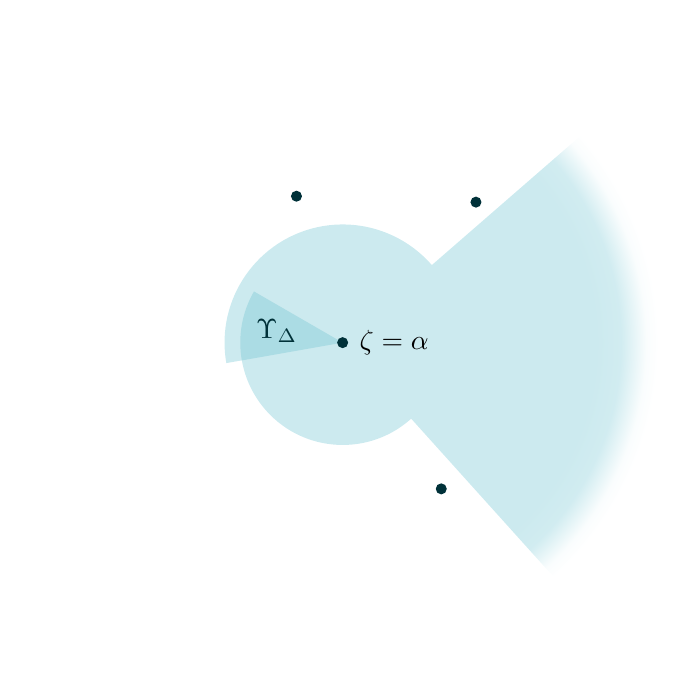
\begin{tikzpicture}
  \newcommand{\spill}{4}
  \fill[ietcoast!20, bezier bounding box, path fading=radial edge]
    (-\spill, -\spill) (\spill, \spill)
    (190:1.5) arc (190:41:1.5) -- (41:\spill) arc (41:-48:\spill) -- (-48:1.3) arc (-48:-170:1.3) -- cycle;
  \fill[ietcoast!33] (0, 0) -- (-170:1.3) arc (-170:-210:1.3) -- cycle;
  \fill[ietcoast!33!black] circle (0.7mm) node[anchor=west, black, outer sep=1mm] {$\zeta = \alpha$};
  \node[ietcoast!33!black] at (-190:0.85) {$\Upsilon_\Delta$};
  \foreach \p in {(107.5:1.95), (46.5:2.46), (-56:2.24)} {
    \fill[ietcoast!33!black] \p circle (0.7mm);
  }
\end{tikzpicture}
\captionof{figure}{The domain $\Upsilon$ at $\zeta=\alpha$.}\label{fig:domain_Upsilon}
\end{center}
For any $\sigma \in \R$, $\Lambda \in \R$, and non-integer $\rho \ge \sigma$, the intersection
\[ \zeta^\rho\,\mathcal{O}_{\zeta = 0} \cap \singexp{\sigma}{\Lambda}(\Upsilon) \]
is a closed subspace of $\singexp{\sigma}{\Lambda}(\Upsilon)$.
\end{lemma}
\begin{proof}
Each point $b \in \Upsilon_\Delta$ has two preimages $b_+, b_- \in \Upsilon$, where $b_+$ is $2\pi$ counterclockwise of $b_-$ around $\zeta = \alpha$. The {\em variation} operator $\var \maps \singexp{\sigma}{\Lambda}(\Upsilon) \to \singexp{\sigma}{\Lambda}(\Upsilon_\Delta)$, defined by\footnote{The target of the variation operator is a space of functions on $\Upsilon_\Delta$ because the variation is defined only on the overlap. Our notation follows the convention of \cite{diverg-resurg-i}, described before Definition~6.46.}
\[ \var \varphi \big|_b = \varphi(b_+) - \varphi(b_-) \]
is bounded. A function in $\singexp{\sigma}{\Lambda}(\Upsilon)$ descends and extends to a function on a neighborhood of $\zeta = 0$ in $\C$ if and only if it lies in the kernel of $\var - (e^{2\pi i \rho} - 1)$. This operator is bounderd, so its kernel is closed.
\end{proof}

Taylor expansion and summation form a two-way link between holomorphic functions and formal power series. For regular enough functions, the formal Laplace transform preserves a one-way vestige of this link: it turns Taylor expansions on the position domain into asymptotic expansions on the frequency domain. \begin{todo}[Compare with Sokal's version of the Watson--Nevanlinna theorem?]\end{todo}
\begin{lemma}\label{lem:laplace-bridge}
Let $\Omega$ be an open sector with $\zeta = 0$ at its tip, and an opening angle of $\pi$ or less\begin{todo}, as illustrated on the position-domain side of Figure~\ref{fig:sectorial_domain-pos-fre} [is it really that helpful to have a picture of this?]\end{todo}. Take some $\rho \in (-1,\infty)$. If $\varphi \in \singexp{\rho}{\Lambda}(\Omega)$ is the sum of a power series $\series{\varphi} \in \zeta^\rho\,\C\{\zeta\}$, then its Laplace transform $\Phi = \laplace_{\zeta, 0}^\theta \varphi$ is asymptotic to the formal Laplace transform $\series{\Phi} = \laplace_{\zeta, 0} \series{\varphi}$.
\end{lemma}
\begin{remark}
This result is similar to Theorem~5.20 of \cite{diverg-resurg-i}. It is weaker in that it does not establish Gevrey asymptoticity, but stronger in that it can be applied to functions with fractionally shifted Taylor expansions.
\end{remark}
\begin{proof}
By adding points within the disk around $\zeta = 0$ where $\series{\varphi}$ converges, expand $\Omega$ to an open set $\Upsilon \subset \widetilde{\C^\times}$ of the kind used in Lemma~\ref{lem:shifted_holo_closed}, Figure~\ref{fig:domain_Upsilon}. Write $\series{\varphi}$ out in the form
\[ \series{\varphi} = a_0 \frac{\zeta^\rho}{\Gamma(\rho+1)} + a_1 \frac{\zeta^{\rho+1}}{\Gamma(\rho+2)} + a_2 \frac{\zeta^{\rho+2}}{\Gamma(\rho+3)} + a_3 \frac{\zeta^{\rho+3}}{\Gamma(\rho+4)} + \ldots, \]
observing that
\[ \series{\Phi} = \frac{a_0}{z^{\rho+1}} + \frac{a_1}{z^{\rho+2}} + \frac{a_2}{z^{\rho+3}} + \frac{a_3}{z^{\rho+4}} + \ldots. \]
For each $n \in \Z_{\ge 0}$, define the tail sum $\varepsilon_n \in \singexp{\sigma+n}{\Lambda}(\Upsilon)$ by the equation
\[ \varphi = a_0 \frac{\zeta^\rho}{\Gamma(\rho+1)} + a_1 \frac{\zeta^{\rho+1}}{\Gamma(\rho+2)} + \ldots + a_{n-1} \frac{\zeta^{\rho+n-1}}{\Gamma(\rho+n)} + \varepsilon_n. \]
Taking the Laplace transform of both sides, we learn that
\[ \Phi = \frac{a_0}{z^{\rho+1}} + \frac{a_1}{z^{\rho+2}} + \ldots + \frac{a_{n-1}}{z^{\rho+n}} + E_n, \]
where $E_n = \laplace_{\zeta, 0}^\theta \varepsilon_n$. To show that $\Phi$ is asymptotic to $\series{\Phi}$, we just need to prove that $|z^{\rho+n} E_n| \to 0$ as $|z| \to \infty$ along every ray.

Because of the conditions we put on $\Omega$, we can apply Proposition~\ref{prop:laplace-cont}, which tells us that $E_n$ lies in $\dualsingexp{-\rho-n-1}(\widehat{\Omega}_0^\Lambda)$. This means that $|E_n| \lesssim \Delta^{-\rho-n-1}$, where $\Delta$ is the distance to the boundary of $\widehat{\Omega}_\alpha^\Lambda$. Noting that \begin{revised}$|z|/\Delta$ goes to a constant limit as $z \to \infty$ along any ray \begin{todo}[check]\end{todo}\end{revised},\footnote{The constant limit is not uniform over all rays, so we are showing that $\Phi$ is asymptotic, but not necessarily uniformly asymptotic, to $\series{\Phi}$.} we deduce that
\begin{align*}
|z^{\rho+n} E_n| & \lesssim |z|^{\rho+n} \Delta^{-\rho-n-1} \\
& = \big(|z|/\Delta\big)^{\rho+n} \Delta^{-1} \\
& \lesssim \Delta^{-1}
\end{align*}
along any ray. This, as discussed above, proves the desired result.
\end{proof}
\color{black}

%The space of $1$-Gevrey formal series is a $\C$-algebra with unit $1$, thus in order to prove that $\borel_\zeta$ is an algebra homomorphism between $\C\llbracket z^{-1}\rrbracket_1$ and $\C\lbrace\zeta\rbrace$ we should endow $\C\lbrace\zeta\rbrace$ with the convolution product and with the formal unit $\delta\defeq\borel_\zeta 1$. 

%Let $\series{\Phi}, \series{\Psi}\in \C \llbracket z^{-1} \rrbracket_1$ (where we assume they are series on the fiber over $\zeta=0$), then 
%\[\borel_\zeta(\series{\Psi}\series{\Phi})=:\series{\psi}\ast\series{\phi}.\]
%In addition, as proved in \cite[Definition 5.12 and Lemma 5.14]{diverg-resurg-i}, the convolution product $\ast$ can be explicitly characterized as \textcolor{orange}{[maybe just define it on holomorphic functions first, and then extend to all formal series by linearity via Taylor series]}
%\[
 %   \series{\psi}\ast\series{\phi}=\int_0^{\zeta}d\zeta' \series{\psi}(\zeta-\zeta')\series{\phi}(\zeta').
%\]
%\begin{lemma}
%The convolution product induces an algebra structure on the space $\singexp{\sigma}{\Lambda}(\Omega)$.
%\end{lemma}
%\begin{proof}
%    Let $\series{\phi},\series{\psi}\in\singexp{\sigma}{\Lambda}(\Omega)$, then a simple computation shows $\series{\phi}\ast\series{\psi}\in\singexp{\sigma}{\Lambda}(\Omega)$.
%\begin{verify}
 %   \begin{align*}
  %      | \series{\phi}\ast\series{\psi}|&=\left|\int_0^\zeta\series{\phi}(\zeta-\zeta')\series{\psi}(\zeta')\, d\zeta'\right|\\
   %     &\le \int_0^\zeta |\series{\phi}(\zeta-\zeta')||\series{\psi}(\zeta')|\, d\zeta'\\
    %    &\le ||\series{\psi}||_{\sigma,\Lambda} \int_0^\zeta\series{\phi}(\zeta-\zeta')|\zeta'|^{\sigma}e^{\Lambda|\zeta'|}\, d\zeta'\\
    %    &\le ||\series{\psi}||_{\sigma,\Lambda} |\zeta|^{\sigma}e^{\Lambda|\zeta|} \int_0^\zeta\series{\phi}(\zeta-\zeta')|\zeta-\zeta'|^{\sigma}e^{\Lambda|\zeta-\zeta'|}\, d\zeta'\\
    %    &\le |\zeta|^{\sigma}e^{\Lambda|\zeta|} ||\series{\psi}||_{\sigma,\Lambda} ||\series{\phi}||_{\sigma,\Lambda}. 
    %\end{align*}
%\end{verify}
%\end{proof}
%We deduce that also the Laplace transform is a $\C$-algebra homomorphism from $\singexp{\sigma}{\Lambda}(\Omega)$ to the space of holomorphic functions on $H_\theta$.  
%\begin{prop}
 %   Let $\sigma>-1$, $\Lambda>0$ and $\theta\in [0,2\pi)$. Then the Laplace transform $\laplace_{\zeta,0}^\theta$ is $\C$-algebra homomorphism from $\singexp{\sigma}{\Lambda}(\Omega)$ to $\mathcal{O}(H_\theta)$. 
%\end{prop}
%\begin{proof}
%First of all, from the properties of $\laplace_{\zeta,0}^\theta$ we know that if $\phi, \psi\in\singexp{\sigma}{\Lambda}(\Omega)$, then
%\[\laplace_{\zeta,0}^\theta\big[{\phi}\ast{\psi}\big]=\laplace_{\zeta,0}^\theta\big[{\phi}\big]\laplace_{\zeta,0}^\theta\big[{\psi}\big],\]
%see for instance \cite[Theorem 2.39]{laplace-tfm}. Then we should prove that $\delta$ is a unit: from its definition and the fact that $\borel_\zeta$ is the formal inverse of $\laplace_{\zeta,0}$, we deduce that 
 %   \[
%\laplace_{\zeta,0}^\theta\big[\delta\big]:=\laplace_{\zeta,0}^\theta\big[\borel_\zeta(1)\big]=1.
 %   \]
%Thus, $\delta$ behaves as a Dirac delta distribution acting on $\singexpalg{\sigma}(\Omega)$. Then, if ${\phi}\in\singexp{\sigma}{\Lambda}(\Omega)$
  %   \begin{align*}
%\big[\delta\ast\phi\big](p)&=\int_0^{\zeta(p)} \delta(\zeta(p)-\zeta)\phi(\zeta) \, d\zeta=\phi(p)
 %   \end{align*}
%\end{proof}
%
%
\subsection{Action on fractional derivatives and fractional integrals}\label{sec:frac-diff-laplace}
In this section, we will consider the action of $\borel_\zeta$ and $\laplace_{\zeta,0}$ with respect to the action of derivatives in both the frequency and position domains, as well as fractional integrals and derivatives $\fracderiv{\lambda}{\zeta}{0}$ in the position domain. This will be useful in Section~\ref{sec:examples}. 

In our treatmeant, we will restrict the Borel transform to the space of $1$-Gevrey series and the Laplace transform to $\singexp{\sigma}{\Lambda}(\Omega_\alpha)$ with $\sigma>-1$ and $\Lambda>0$, for some domain $\Omega_\alpha$ as in Figure~\ref{fig:sectorial_domain-pos-fre}.
\begin{definition}
For $\nu \in (-\infty, 1)$, the \textit{fractional integral} $\partial^{\nu-1}_{\zeta, \alpha}$ is defined by
\[ [\partial^{\nu-1}_{\zeta, \alpha} \phi] \defeq \frac{1}{\Gamma(1-\nu)} \int_{\mathcal{S}'(\zeta)} \big(\zeta-\zeta'\big)^{-\nu} \phi' \,d\zeta', \]
where $\mathcal{S}'(\zeta)$ is the line segment from $\zeta'=\alpha$ to $\zeta'=\zeta$.%\footnote{\textcolor{magenta}{Why highlight this special case of the definition above? Is it important to use $\lambda$ instead of $\nu-1$?} For completeness we also give the \textcolor{magenta}{[redundant] definition} of the fractional integral $\partial_{\zeta_\alpha,0}^{-\lambda}$: 
% \begin{equation*}
%     \partial_{\zeta_\alpha,0}^{-\lambda}\varphi(p)\defeq\frac{1}{\Gamma(\lambda)}\int_{\zeta_\alpha=0}^{p}(\zeta_\alpha(p)-\zeta_\alpha)^{\lambda-1} \varphi \, d\zeta_\alpha.
% \end{equation*}
% }
\end{definition}
Here, we are using Notation~\ref{notn:prod} and taking advantage of the fact that $\zeta'' = \zeta - \zeta'$ along our integration path.

The fractional integral obeys the semigroup law \cite[Section  1.3]{mladenov2014advanced}
\begin{align*}
\fracderiv{\lambda}{\zeta}{\alpha}\,\fracderiv{\mu}{\zeta}{\alpha} & = \fracderiv{\lambda+\mu}{\zeta}{\alpha} \qquad \lambda, \mu \in (-\infty, 0),
\end{align*}
and agrees with ordinary repeated integration when $\nu$ is an integer~\cite[Equation 35]{mladenov2014advanced}.

For $\mu \in (0, 1)$ and integers $n \ge 0$, fractional derivatives $\fracderiv{n+\mu}{\zeta}{0}$ are defined by composing $\fracderiv{\mu-1}{\zeta}{0}$ with powers of $\tfrac{\partial}{\partial \zeta}$. However, $\fracderiv{\mu-1}{\zeta}{0}$ and $\tfrac{\partial}{\partial \zeta}$ do not commute~\cite[equation 54]{mladenov2014advanced}. Various ordering conventions give various definitions of $\fracderiv{n+\mu}{\zeta}{0} \phi$, which differ by operators that act on the germ of $\phi$ at zero (see \cite[Section 1.3]{mladenov2014advanced}---original source \cite{podlubny}). We will use the {\em Riemann-Liouville} convention.
\begin{definition}\label{definition:frac_driv}
For $\mu \in (0, 1)$ and integers $n \ge 0$, the {\em Riemann-Liouville fractional derivative} $\fracderiv{n+\mu}{\zeta}{0}$ is defined by
\[ \fracderiv{n+\mu}{\zeta}{0} \defeq \big(\tfrac{\partial}{\partial \zeta}\big)^{n+1} \fracderiv{\mu-1}{\zeta}{0}. \]
\end{definition}
The symbol $\fracderiv{\mu}{\zeta}{0}$ is now defined for any $\mu \in \R \smallsetminus \{0, 1, 2, 3, \ldots\}$. It denotes a fractional integral when $\mu$ is negative, and a fractional derivative when $\mu$ is a positive non-integer.

The Riemann-Liouville fractional derivative is a left inverse of the fractional integral, in the sense that $\fracderiv{\lambda}{\zeta}{ 0}\,\fracderiv{-\lambda}{\zeta}{0}$ is the identity for all $\lambda \in (0, \infty)$. This extends the semigroup law:
\begin{align*}
\fracderiv{\lambda}{\zeta}{0}\,\fracderiv{\mu}{\zeta}{0} & = \fracderiv{\lambda+\mu}{\zeta}{0} & \lambda \in \R \smallsetminus \{0, 1, 2, 3, \ldots\},\quad\mu \in (-\infty, 0).
\end{align*}
\begin{revised}
\begin{prop}\label{prop:L-int-op}
For any $\phi\in\singexp{\sigma}{\Lambda}(\Omega)$ with $\sigma>-1$ and $\Lambda>0$, we have
\begin{enumerate}[label=(\roman*)]
\item\label{res:frac-deriv} \textbf{Fractional derivatives}

$\laplace_{\zeta,0} \big[\fracderiv{\mu}{\zeta}{0} \phi\big] = z^{\mu} \laplace_{\zeta,0} \phi$ for every $\mu\in(0,1)$;
\item\label{res:frac-int} \textbf{Fractional integrals}

$\laplace_{\zeta,0} \big[\fracderiv{\lambda}{\zeta}{0} \phi\big] = z^{\lambda} \laplace_{\zeta,0} \phi$ for every $\lambda\in(-\infty,0)$;
\item\label{res:whole-deriv} \textbf{Whole derivatives}

$\laplace_{\zeta,0} \big[\big(\frac{\partial}{\partial\zeta}\big)^n \phi\big] = z^{n} \laplace_{\zeta,0} \phi$ for all $n\in\{1, 2, 3, \ldots\}$, under the condition that $\phi^{(0)}, \phi^{(1)}, \ldots, \phi^{(n)}$ all vanish at $\zeta = 0$;
\item\label{res:monom-mult} \textbf{Monomial multiplication}

$\laplace_{\zeta,0} \big[\zeta^n \phi\big] = \big(-\frac{\partial}{\partial z}\big)^n \laplace_{\zeta,0} \phi$ for every $n\in\{0,1,2,3,\ldots\}$.
\end{enumerate}
\end{prop}
\end{revised}
\begin{proof}
%where in the last step we repetedly use integration by part and the fact that boundary terms vanish. %Then we deduce that   
%\begin{align*}
 %   z^\mu\laplace_{\zeta,0}\phi&= \laplace_{\zeta,0}\Big[\frac{\zeta^{-\alpha-1}}{\Gamma(-\alpha)}\Big] \laplace_{\zeta,0}\big[\partial_\zeta^n \phi\big]\\
  %  &=\laplace_{\zeta,0}\Big[\frac{\zeta^{-\alpha-1}}{\Gamma(-\alpha)}\ast \partial_\zeta^n\phi\Big]\\
   % &=z^n\laplace_{\zeta,0}\Big[\fracderiv{\lambda}{\zeta}{0}\partial_\zeta^n \phi\Big]
%\end{align*}
   
Results \ref{res:frac-deriv} and \ref{res:frac-int} follow from the properties of the Laplace transform with respect to the convolution product. For every $\tau \in (-\infty, 0) \cup (0,1)$,
\begin{align*}
z^\tau\laplace_{\zeta,0}\phi&=\laplace_{\zeta,0}\Big[\frac{\zeta^{-\tau-1}}{\Gamma(-\tau)}\Big] \laplace_{\zeta,0}\phi\\
&=\laplace_{\zeta,0}\Big[\frac{\zeta^{-\tau-1}}{\Gamma(-\tau)} \ast_\zeta \phi\Big] \\
&=\laplace_{\zeta,0} \int_{\substack{\mathcal{S}'(\zeta) \times \mathcal{S}''(\zeta) \\ \zeta' + \zeta'' = \zeta}}\frac{(\zeta'')^{-\tau-1}}{\Gamma(-\tau)} \phi' d\zeta'\\
&=\laplace_{\zeta,0} \int_{\substack{\mathcal{S}'(\zeta) \times \mathcal{S}''(\zeta) \\ \zeta' + \zeta'' = \zeta}}\frac{(\zeta-\zeta')^{-\tau-1}}{\Gamma(-\tau)} \phi' d\zeta'\\
&=\laplace_{\zeta,0}\fracderiv{\tau}{\zeta}{0}\phi,
\end{align*}
where $\mathcal{S}'(\zeta)$ is the line segment from $\zeta'=0$ to $\zeta' = \zeta$, $\mathcal{S}''(\zeta)$ is the line segment from $\zeta''=\zeta$ to $\zeta''=0$, and we are taking advantage of the fact that $\zeta'' = \zeta - \zeta'$ on the integration path. Result~\ref{res:whole-deriv} is proven by repeated integration by parts, with the condition on $\phi^{(0)}, \phi^{(1)}, \ldots \phi^{(n)}$ ensuring that the boundary terms vanish:
\begin{align*}
    z^n\laplace_{\zeta,0}\phi&=\int_0^\infty e^{-z\zeta} z^n \phi \, d\zeta\\
    &=(-1)^n\int_0^\infty \partial_\zeta^n \big[e^{-z\zeta}\big]  \phi\, d\zeta\\
    &=\laplace_{\zeta,0}\big[\partial_\zeta^n \phi\big].
\end{align*}
Result~\ref{res:monom-mult} is also proven by repeated integration by parts, with the assumption that $\zeta^n\phi\in\singexp{\sigma}{\Lambda}(\Omega)$ ensuring that the integral converges.
        %from a 2d integration argument, akin to the one in \cite[Theorem~2.39]{laplace-tfm}. This generalizes the Laplace transform's action on derivatives: using differentiation under the integral we prove \emph{ii)} (see also \cite[Theorem~1.34]{laplace-tfm}). Similarly, one can prove \emph{iii)}.  
\end{proof}
\begin{lemma}\label{lem:frac-deriv-Borel}
For any non-integer $\mu \in (0, \infty)$ and any integer $k \ge 0$,
\[ \partial^\mu_{\zeta } \borel_\zeta \big[z^{-(k+1)}\big] =  \borel_\zeta \big[z^\mu z^{-(k+1)}\big]. \]
\end{lemma}
\begin{proof}
We will show that for any $\mu \in (0, 1)$ and any integer $n \ge 0$, the claim holds with $\mu = n + \alpha$. First, evaluate
\begin{align*}
\partial^{\mu-1}_{\zeta} \borel_\zeta \big[z^{-(k+1)}\big] & = \frac{1}{\Gamma(1-\mu)} \int_0^\zeta (\zeta-\zeta')^{-\mu} \frac{(\zeta')^k}{\Gamma(k+1)}\,d\zeta' \\
& = \frac{1}{\Gamma(1-\mu)\,\Gamma(k+1)} \int_0^1 (\zeta-\zeta t)^{-\mu} (\zeta t)^k\,\zeta\,dt \\
& = \frac{\zeta^{k-(\mu-1)}}{\Gamma(1-\mu)\,\Gamma(k+1)} \int_0^1 (1-t)^{-\mu} t^k\,dt \\
& = \frac{\zeta^{k-(\mu-1)}}{\Gamma\big(k-(\mu-1)+1\big)}
\end{align*}
by reducing the integral to Euler's beta function (see \cite[Identity 5.12.1]{dlmf}). This establishes that
\begin{equation}\label{frac-diff-laplace}
\big(\tfrac{\partial}{\partial \zeta}\big)^{n+1}\,\partial^{\mu-1}_{\zeta } \borel_\zeta \big[z^{-(k+1)}\big] = \frac{\zeta^{k-(n+\mu)}}{\Gamma\big(k-(n+\mu)+1\big)}
\end{equation}
for $n = -1$. If \eqref{frac-diff-laplace} holds for $n = m$, it also holds for $n = m+1$, because
\begin{align*}
\tfrac{\partial}{\partial \zeta} \big(\tfrac{\partial}{\partial \zeta}\big)^{m+1}\,\partial^{\mu-1}_{\zeta} \borel_\zeta \big[z^{-(k+1)}\big] & = \frac{\partial}{\partial \zeta} \left( \frac{\zeta^{k-(m+\mu)}}{\big(k-(m+\mu)\big)\,\Gamma\big(k-(m+\mu)\big)} \right) \\
& = \frac{\zeta^{k-(m+1+\mu)}}{\Gamma\big(k-(m+\mu)\big)}
\end{align*}
Hence, \eqref{frac-diff-laplace} holds for all $n \ge -1$, and the desired result quickly follows. The condition $\mu \in (0, 1)$ saves us from the trouble we would run into if $k-(m+\mu)$ were in $\Z_{\le 0}$. This is how we avoid the initial value corrections that appear in ordinary derivatives of Borel transforms.
\end{proof}
We can now prove the properties of the Borel transform analogous to the one of the Laplace transform from Proposition~\ref{prop:L-int-op}.
\begin{revised}
\begin{prop}\label{prop:frac-der-int-borel}
Let for any $1$-Gevrey series $\series{\Phi}\in\C\llbracket z^{-1}\rrbracket_1$, we have
\begin{enumerate}[label=(\roman*)]
\item\label{res:frac-deriv-borel} \textbf{Fractional derivatives}

$\borel_\zeta\big[ z^\mu \, \series{\Phi}\big]=\fracderiv{\mu}{\zeta}{0}\, \borel_\zeta\series{\Phi}$ for every $\mu\in(0, \infty)$;
\item\label{res:frac-int-borel} \textbf{Fractional integrals}

$\borel_\zeta\big[z^\lambda\, \series{\Phi}\big]=\fracderiv{\lambda}{\zeta}{0}\,\borel_\zeta\series{\Phi}$ for every $\lambda\in(-\infty, 0)$;
\item\label{res:whole-deriv-borel} \textbf{Whole derivatives}

$\borel_\zeta\big[\partial_z^{k} \series{\Phi}\big]=(-\zeta)^k\borel_\zeta\series{\Phi}$ for all $k\in\{0, 1, 2, 3, \ldots\}$, under the condition that $\series{\Phi}\in z^{-k-1}\llbracket z^{-1}\rrbracket_1$.\footnote{This property holds for all series in $\C\llbracket z^{-1}\rrbracket$, even ones that are not $1$-Gevrey.}
\end{enumerate} 
\end{prop}
\begin{proof} 
Result~\ref{res:frac-deriv-borel} follows from Lemma~\ref{lem:frac-deriv-Borel}. 

To prove result~\ref{res:frac-int-borel}, first notice that for $\lambda \in \R_{< 0}$,
\[\fracderiv{\lambda}{\zeta}{0}\zeta^{k}=\zeta^{k-\lambda}\frac{k!}{\Gamma(k-\lambda+1)}.\] 
Then, given a series $\series{\Phi} = \sum_{n\geq 0} a_n z^{-n}$, we compute
\begin{align*}
\borel_\zeta \big[z^\lambda \series{\Phi}\big] & = \sum_{n\geq 0}a_n\frac{\zeta^{n-\lambda}}{\Gamma(n-\lambda+1)} \\
& = \sum_{n\geq 0}a_n\frac{\zeta^{n-\lambda}}{n!}\frac{n!}{\Gamma(n-\lambda+1)} \\
& = \sum_{n\geq 0} \frac{a_n}{n!}\,\fracderiv{\lambda}{\zeta}{0}\zeta^n \\
& = \fracderiv{\lambda}{\zeta}{0}\series{\Phi}.
\end{align*}
using the fact that $\borel_\zeta\series{\Phi}$ is convergent in the last step.

Finally, result~\ref{res:whole-deriv-borel} follows from a simple computation: 
\begin{align*}
\borel_\zeta\big[\partial_z^k\series{\Phi}\big]&=\borel_\zeta\left[\sum_{n=k+1}^\infty a_n \frac{(n+k-1)!}{(n-1)!} (-1)^{k} z^{-n-k}\right]\\
&=(-1)^k \sum_{n=k+1}^\infty a_n \frac{(n+k-1)!}{(n-1)!}\frac{\zeta^{n+k-1}}{(n+k-1)!}\\
&=(-\zeta)^k\sum_{n=k+1}^\infty a_n \frac{\zeta^{n-1}}{(n-1)!}\\
&=(-\zeta)^k\borel_\zeta \series{\Phi}.
\end{align*}
\end{proof}
\end{revised}
%
\section{Proof of main results}\label{sec:proof_main_results}
%
\subsection{Borel regularity for ODEs}\label{borel_reg-ODE}
In Section~\ref{sec:regularity-results}, we show that linear level~1 ODEs of a certain form always have Borel regular solutions, indexed by the characteristic roots of their constant-coefficient parts. These solutions turn out to be asymptotic to the formal series solutions found by Poincar\'{e}.

In Section~\ref{sec:new-summability-proof}, we will look at the same class of ODEs from a more formal perspective, starting from the assumption that Poincar\'{e}'s solutions exist and their Borel transforms converge. Using the existence and uniqueness results that characterize the Borel regular solutions, we give a new proof that Poincar\'{e}'s solutions are Borel summable.
%
\subsubsection{Regularity results}\label{sec:regularity-results}
Let us recall the setting from Section~\ref{borel-reg:explanatory-power}. Let $\mathcal{P}$ be a linear differential operator of the form 
\begin{equation}\label{eqn:operator-P}
\mathcal{P} = P\big(\tfrac{\partial}{\partial z}\big) + \frac{1}{z} Q\big(\tfrac{\partial}{\partial z}\big) + \frac{1}{z^2} R(z^{-1}),
\end{equation}
where
\begin{enumerate}
\item $P$ is a monic degree-$d$ polynomial whose roots are all simple; 
\item $Q$ is a degree-$(d-1)$ polynomial that is non-zero at every root of $P$;
\item $R(z^{-1})$ is holomorphic in some disk $|z| > A$ around $z = \infty$. In particular, the power series
\[ R(z^{-1}) = \sum_{j=0}^\infty R_j z^{-j} \]
converges in the region $|z| > A$.
\end{enumerate}
%%For each root $-\alpha$ of $P$, choose an open sector $\Omega_\alpha \subset \C$ that has $\zeta = \alpha$ at its tip, does not touch any other root of $P(-\zeta)$, and has an opening angle of $\pi$ or less.
For each root $-\alpha$ of $P$, let $\hat{\mathcal{P}}_{\alpha}$ be the Volterra operator 
\begin{equation}\label{eq:hat_P}
    \hat{\mathcal{P}}_\alpha:=P(-\zeta)+\partial_{\zeta,\alpha}^{-1}\circ Q(-\zeta)+\partial_{\zeta,\alpha}^{-2}\circ R(\partial_{\zeta,\alpha}^{-1})
\end{equation}
From Lemma~2 in~\cite{reg-sing-volterra}, we know that if $\psi_\alpha$ satisfies the equation $\hat{\mathcal{P}}_\alpha\psi_\alpha=0$, then its Laplace transform $\Psi_\alpha:=\laplace_{\zeta,\alpha}^{\theta}\psi_\alpha$ satisfies the equation $\mathcal{P}\Psi_\alpha=0$, as long as the Laplace transform is well-defined. \begin{todo}[Transition text]\end{todo}
%%%\begin{itemize}
%%%\item The set $\Omega_\alpha$ is star-shaped around $\zeta = \alpha$. In other words, for any $a \in \Omega_\alpha$, a straight path from $\zeta = \alpha$ to $a$ stays in $\Omega_\alpha$. Since $\Omega_\alpha$ does not contain $\zeta = \alpha$, we will always leave that starting point out of the path.
%%%\item The set $\Omega_\alpha$ does not contain the tubular neighborhood of the other critical points, as shown in Figure \ref{Fig:domain}. \textcolor{orange}{[In ``Regular singular Volterra,'' we assume that $\Omega_\alpha$ does not touch any other critical point (that is, does not contain any other critical point in its closure). Under the star-shaped assumption, I think that implies avoiding tubular neighborhoods of the shadow rays.]}
%%%\end{itemize}
\begin{theorem}[restatement of \ref{thm:exist_uniq_ODE}]\label{re:thm:exist_uniq_ODE}
Choose a root $-\alpha$ of $P$. Choose an open sector $\Omega_\alpha$ which has an opening angle of $\pi$ or less, has $\zeta = \alpha$ at its tip, and does not touch any other root of $P(-\zeta)$. The equation $\mathcal{P}\Psi = 0$ has a unique solution $\Psi_\alpha$ in the affine subspace
\[ e^{-\alpha z} \left[ z^{-\tau_\alpha} + \dualsingexp{-\tau_\alpha-1}(\widehat{\Omega}_\alpha^\bullet) \right] \]
\begin{todo}[\textbf{A} define $\widehat{\Omega}_\alpha^\bullet$]\end{todo} of the space $e^{-\alpha z} \dualsingexp{-\tau_\alpha}(\widehat{\Omega}_\alpha^\bullet)$ from Section~\ref{sec:reg-decay}.
\end{theorem}
\begin{center}
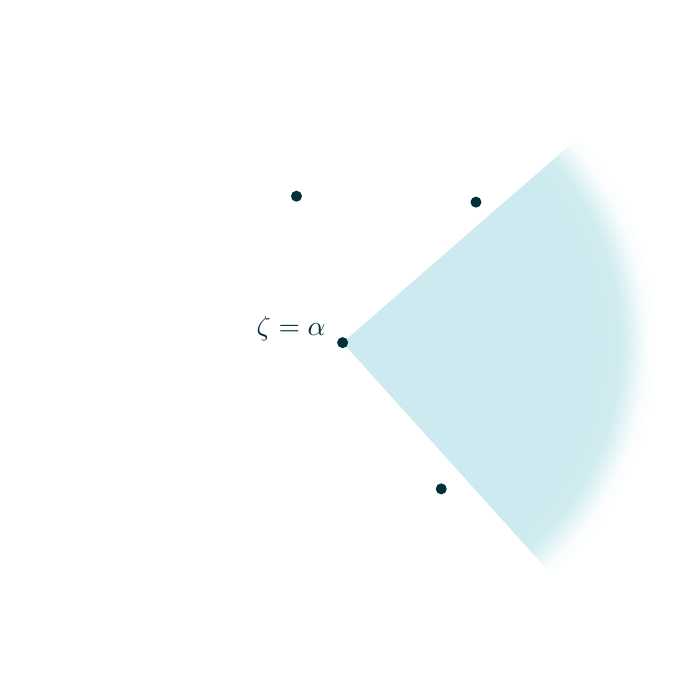
\begin{tikzpicture}
\newcommand{\spill}{4}
\fill[ietcoast!20, bezier bounding box, path fading=radial edge]
  (-\spill, -\spill) (\spill, \spill)
  (0, 0) -- (41:\spill) arc (41:-48:\spill) -- cycle;
\fill[ietcoast!33!black] circle (0.7mm) node[anchor=-15, outer sep=1mm] {$\zeta = \alpha$};
\foreach \p in {(107.5:1.95), (46.5:2.46), (-56:2.24)} {
  \fill[ietcoast!33!black] \p circle (0.7mm);
}
\end{tikzpicture}
\captionof{figure}{The sectorial domain $\Omega_\alpha$.}\label{fig:sectorial_domain--with roots P}
\end{center}
\begin{proof}
After rescaling by a constant, Theorem~4 of \cite{reg-sing-volterra} tells us that the equation $\hat{\mathcal{P}}_\alpha \psi_\alpha = 0$ has a unique solution $\psi_\alpha$ in the affine subspace
\[ \frac{\zeta^{\tau_\alpha-1}}{\Gamma(\tau_\alpha)} + \singexpalg{\tau_\alpha}(\Omega_\alpha) \]
of the space $\singexpalg{\tau_\alpha-1}(\Omega_\alpha)$. The same is true on any smaller sector created by shaving a sector off each edge of $\Omega_\alpha$. By Theorem~\ref{translation} and the results of Section~\ref{sec:reg-decay}, the Laplace transform $\laplace^\theta_{\zeta, \alpha}$ is a left-invertible map
\[ \singexpalg{\tau_\alpha}(\Omega_\alpha) \to e^{-\alpha z} \dualsingexp{-\tau_\alpha-1}(\widehat{\Omega}_\alpha^\bullet). \]
With $\Psi_\alpha = \laplace^\theta_{\zeta, \alpha} \psi_\alpha$, the desired result follows.
\end{proof}
\begin{todo}[Add flavor text]\end{todo}
\begin{theorem}[restatement of \ref{thm:soln_is_Borel_sum}]\label{re:thm:soln_is_Borel_sum}
The analytic solution $\Psi_\alpha$ from Theorem~\ref{thm:exist_uniq_ODE} is the Borel sum of a formal trans-monomial solution $\series{\Psi}_\alpha \in e^{-\alpha z} z^{-\tau_\alpha}\,\C \llbracket z^{-1} \rrbracket$ of the equation $\mathcal{P}\series{\Phi} = 0$.
\end{theorem}
\begin{proof}
Take an open sector $\Omega_\alpha$ of the kind used in Theorem~\ref{re:thm:exist_uniq_ODE}, and expand it to an open set $\Upsilon \subset \widetilde{\C^\times}$ of the kind used in Lemma~\ref{lem:shifted_holo_closed}. Our arguments in \cite{reg-sing-volterra} took place on $\C$, but they work just as well on a covering space like $\widetilde{\C^\times}$. We can therefore use Theorem~4 of \cite{reg-sing-volterra} to show that $\hat{\mathcal{P}}_\alpha \psi_\alpha = 0$ has a unique solution $\psi_\alpha$ in the affine subspace 
\[ \frac{\zeta_\alpha^{\tau_\alpha-1}}{\Gamma(\tau_\alpha)} + \singexpalg{\tau_\alpha}(\Upsilon) \]
of the space $\singexpalg{\tau_\alpha-1}(\Upsilon)$. Restricting this solution to $\Omega_\alpha$ gives the analogous solution from the proof of Theorem~\ref{re:thm:exist_uniq_ODE}, as we can see from the uniqueness part of Theorem~4 of \cite{reg-sing-volterra}. To express $\Psi_\alpha = \laplace_{\zeta, \alpha} \psi_\alpha$ as the Borel sum of a trans-monomial, we first need to expess $\psi_\alpha$ as the sum of a convergent power series. We will do this by showing that $\psi_\alpha$ lies in $\zeta_\alpha^{\tau_\alpha - 1}\,\mathcal{O}(\pi \Upsilon)$.

For convenience, let $p = P(-\zeta)$ and $q = Q(-\zeta)$. To prove Theorem~4 in \cite{reg-sing-volterra}, we rewrite the equation $\hat{\mathcal{P}}_\alpha \solwhole = 0$ as a regular singular Volterra equation $\solwhole = \volterra^\alpha \solwhole$ that satisfies the conditions of the underlying existence and uniqueness result~\cite[Theorem~3]{reg-sing-volterra}. The operator $\volterra^\alpha$ is the sum of the ``prototypical'' part
%%\[ \hardpart^\alpha = -\tfrac{1}{P(-\zeta)} \circ \partial^{-1}_{\zeta, \alpha} \circ Q(-\zeta) \]
\[ \hardpart^\alpha = -\tfrac{1}{p} \circ \partial^{-1}_{\zeta, \alpha} \circ q \]
and the perturbation
%%\[ \softpart^\alpha = \tfrac{1}{P(-\zeta)} \circ \partial^{-2}_{\zeta, \alpha} \circ R(\partial^{-1}_{\zeta, \alpha}) \]
\[ \softpart^\alpha = \tfrac{1}{p} \circ \partial^{-2}_{\zeta, \alpha} \circ R\big(\partial^{-1}_{\zeta, \alpha}\big). \]

Let us run through the proof of Theorem~3, specialized to the case we consider in Theorem~4. First, picking an arbitrary point $b \in \Omega_\alpha$, we show that the {\em prototype solution}
\[ \solproto(a) = \frac{1}{p(a)} \exp\left(-\int_{b}^{a}\frac{q}{p}\;d\zeta_\alpha\right) \]
lies in the space $\singexpalg{\tau_\alpha - 1}(\Upsilon)$ and satisfies the equation $\solproto = \hardpart^\alpha \solproto$. We then look for a perturbation $\solptb$ that makes $\solwhole = \solproto + \solptb$ a solution of the Volterra equation we are trying to solve. This is equivalent to solving the inhomogeneous equation
\begin{equation}\label{eqn:inhomog-volterra}
\solptb = \softpart^\alpha \solproto + \volterra^\alpha \solptb
\end{equation}
The central idea of the proof is to show that $\softpart^\alpha$ maps $\solproto$, and in fact all of $\singexpalg{\tau_\alpha - 1}(\Upsilon)$, into $\singexpalg{\tau_\alpha}(\Upsilon)$, and that $\volterra^\alpha$ is a contraction of $\singexp{\tau_\alpha}{\Lambda}(\Upsilon)$ when $\Lambda$ is large enough. It follows, by the contraction mapping theorem, that equation~\eqref{eqn:inhomog-volterra} has a unique solution $\solptb$ in $\singexp{\tau_\alpha}{\Lambda}(\Upsilon)$. More explicitly, we can solve equation~\eqref{eqn:inhomog-volterra} by fixed-point iteration. Defining
\begin{align*}
\solptb^{(0)} & = \softpart^\alpha \solproto \\
\solptb^{(1)} & = \softpart^\alpha \solproto + \volterra^\alpha \solptb^{(0)} \\
\solptb^{(2)} & = \softpart^\alpha \solproto + \volterra^\alpha \solptb^{(1)} \\
\solptb^{(3)} & = \softpart^\alpha \solproto + \volterra^\alpha \solptb^{(2)} \\
& \;\;\vdots
\end{align*}
we get a sequence of functions that converges in $\singexp{\tau_\alpha}{\Lambda}(\Upsilon)$ to a solution $f_*$.

In \citesection{sec:construction} Section~3.2.1 of \cite{reg-sing-volterra}, we rewrite the prototype solution in the form
\[ \solproto(a) = \frac{1}{p(a)} \left(\frac{\zeta_\alpha(a)}{\zeta_\alpha(b)}\right)^{\tau_\alpha} \exp\left[-\int_b^a \left( \frac{q}{p} + \frac{\tau_\alpha}{\zeta_\alpha} \right)\;d\zeta_\alpha\right], \]
which shows that it represents a germ in $\zeta_\alpha^{\tau_\alpha-1}\,\mathcal{O}_{\zeta = \alpha}$. By working with Taylor series, we can show that $\softpart^\alpha$ maps
\[ \zeta_\alpha^{\tau_\alpha-1}\,\mathcal{O}_{\zeta=\alpha} \to \zeta^{\tau_\alpha}\,\mathcal{O}_{\zeta=\alpha} \]
and $\volterra^\alpha$ maps $\zeta_\alpha^{\tau_\alpha}\,\mathcal{O}_{\zeta=\alpha}$ to itself. It follows that the sequence $\solptb^{(0)}, \solptb^{(1)}, \solptb^{(2)}, \ldots$ lies in $\zeta_\alpha^{\tau_\alpha}\,\mathcal{O}_{\zeta=\alpha} \cap \singexp{\tau_\alpha}{\Lambda}(\Upsilon)$, which by Lemma~\ref{lem:shifted_holo_closed} is a closed subspace of $\singexp{\tau_\alpha}{\Lambda}(\Upsilon)$. The limit $f_*$, which satisfies equation~\eqref{eqn:inhomog-volterra}, therefore represents a germ in $\zeta_\alpha^{\tau_\alpha}\,\mathcal{O}_{\zeta = \alpha}$. Recalling that the prototype solution represents a germ in $\zeta_\alpha^{\tau_\alpha-1}\,\mathcal{O}_{\zeta = \alpha}$, we can deduce that $\psi_\alpha$ represents a germ in $\zeta_\alpha^{\tau_\alpha-1}\,\mathcal{O}_{\zeta = \alpha}$ too.

We now cross over into the formal world, expanding $\psi_\alpha$ as a shifted Taylor series $\series{\psi}_\alpha \in \zeta_\alpha^{\tau_\alpha-1}\,\C\{\zeta\}$. By definition, the formal Laplace transform $\series{\Psi}_\alpha = \laplace_{\zeta, \alpha} \series{\psi}_\alpha$ lies in $e^{-\alpha z} z^{-\tau_\alpha}\,\C \llbracket z^{-1} \rrbracket$.

When we take the Borel sum of $\series{\Psi}_\alpha$, we start by retracing the construction steps described above. The Borel transform inverts the formal Laplace transform, bringing us back to $\series{\psi}_\alpha$, and summation then inverts the Taylor expansion, bringing us back to $\psi_\alpha$. We finish the Borel summation by taking the Laplace transform $\laplace^\theta_{\zeta, \alpha} \psi_\alpha$, giving $\Psi_\alpha$ by definition.
\end{proof}
\begin{todo}[Add flavor text]\end{todo}
\begin{corollary}[restatement of \ref{cor:soln_borel-reg}]\label{re:cor:soln_borel-reg}
The analytic solution $\Psi_\alpha$ from Theorem~\ref{re:thm:exist_uniq_ODE} is Borel regular. This is because $\Psi_\alpha$ is asymptotic to the formal solution $\series{\Psi}_\alpha$ from Theorem~\ref{re:thm:soln_is_Borel_sum}.
\end{corollary}
\begin{proof}
In the proof of Theorem~\ref{re:thm:soln_is_Borel_sum}, we showed that the position-domain solution $\psi_\alpha \in \singexpalg{\tau_\alpha-1}(\Upsilon)$ is the sum of a shifted Taylor series $\series{\psi}_\alpha \in \zeta^{\tau_\alpha-1}\,\C\{\zeta\}$. Since $\Psi_\alpha$ is the Laplace transform of $\psi_\alpha$, and $\series{\Psi}_\alpha$ is the formal Laplace transform of $\series{\psi}_\alpha$, Lemma~\ref{lem:laplace-bridge} tells us that $\Psi_\alpha$ is asymptotic to $\series{\Psi}_\alpha$. Taking the Borel sum of $\series{\Psi}_\alpha$ gives us back $\Psi_\alpha$, by construction, so $\Psi_\alpha$ is Borel regular.
\end{proof}
%
\subsubsection{A new proof of the Borel summability of the Poincar\'{e} solutions}\label{sec:new-summability-proof}
%
In~\cite{int-irreg}, Poincar\'{e} described a formal way to solve the equation $\mathcal{P}\series{\Phi} = 0$ for an operator of the form~\eqref{eqn:operator-P}. Choose a root $-\alpha$ of $P$, set $\tau_\alpha = Q(-\alpha)/P'(-\alpha)$, and look for a formal solution $\series{\Psi}_\alpha$ in the space $e^{-z\alpha} z^{-\tau_\alpha}\C\llbracket z^{-1} \rrbracket$. Once the leading coefficient of $\series{\Psi}_\alpha$ is chosen, the rest of the coefficients are determined, and can be found order by order. The Ramis Index Theorem guarantees that $\series{\Psi}_\alpha$ will be $1$-Gevrey~\cite{ramis_index}.

We have come this far in our discussion of Poincar\'{e}'s method through formal reasoning in the frequency domain. From here, there are various ways to show that $\series{\Psi}_\alpha$ is Borel summable. We do it by using Theorem~4 of \cite{reg-sing-volterra} to show that the relevant integral equation in the position domain has a unique analytic solution.
\begin{theorem}\label{thm:summability_ODE}
Choose a root $-\alpha$ of $P$. Choose an open sector $\Omega_\alpha$ which has an opening angle of $\pi$ or less, has $\zeta = \alpha$ at its tip, and does not touch any other root of $P(-\zeta)$. If a $1$-Gevrey trans-monomial $\series{\Psi}_\alpha \in e^{-z\alpha} z^{-\tau_\alpha}\C\llbracket z^{-1} \rrbracket_1$ satisfies the equation $\mathcal{P} \series{\Psi}_\alpha = 0$, then it is Borel summable at $\alpha$ along any ray in $\Omega_\alpha$, and its Borel sum is proportional to the analogous analytic solution $\Psi_\alpha$ from Theorem~\ref{re:thm:exist_uniq_ODE}.
\end{theorem}
\begin{proof}
By Proposition~\ref{prop:frac-der-int-borel}, the Borel transform $\series{\psi}_\alpha = \borel_\zeta \series{\Psi}_\alpha$ is a formal solution of the equation $\hat{\mathcal{P}}_\alpha \series{\psi}_\alpha = 0$, where $\hat{\mathcal{P}}_\alpha$ is the operator\eqref{eq:hat_P}. By Proposition~\ref{prop:gevrey_to_convergent}, the series $\series{\psi}_\alpha$ converges to a holomorphic function $\hat{\psi}_\alpha$ on some open set $\Omega_\text{near}$ created by restricting $\Omega_\alpha$ to a small disk around of $\zeta = \alpha$. Since the integrals in $\hat{\mathcal{P}}_\alpha \hat{\psi}_\alpha$ converge absolutely, $\hat{\psi}_\alpha$ satisfies the same equation that its Taylor series does: $\hat{\mathcal{P}}_\alpha \hat{\psi}_\alpha = 0$.

Since the series $\series{\psi}_\alpha$ lies in $\zeta^{\tau_\alpha-1} \C\{\zeta\}$, the function $\hat{\psi}_\alpha$ lies in $\zeta^{\tau_\alpha-1} \mathcal{O}(\Omega_\text{near})$. Since $\Omega_\text{near}$ is bounded, this implies that $\hat{\psi}_\alpha$ lies in $c \zeta^{\tau_\alpha-1} + \singexpalg{\tau_\alpha}(\Omega_\text{near})$, where $c$ is the leading coefficient of $\series{\psi}_\alpha$. We know from Theorem~4 of \cite{reg-sing-volterra} that the equation $\hat{\mathcal{P}}_\alpha \varphi = 0$ has unique solution in the $\zeta^{\tau_\alpha-1} + \singexpalg{\tau_\alpha}(\Omega_\alpha)$. The same theorem applies on the domain $\Omega_\text{near}$, where its uniqueness provision shows that $\hat{\psi}_\alpha$ and $c\psi_\alpha$ must match. This means, in particular, that $\hat{\psi}_\alpha$ can be analytically continued throughout $\Omega_\alpha$, and it is uniformly of exponential type on that sector. Thus, $\hat{\psi}_\alpha$ has a well-defined Laplace transform along any ray $\mathcal{J}^\theta_{\zeta, \alpha}$ in $\Omega_\alpha$, meaning that $\series{\Psi}_\alpha$ is Borel summable along any such ray. Recalling how the solution $\Psi_\alpha$ was constructed in Theorem~\ref{re:thm:exist_uniq_ODE}, we see that the Borel sum of $\series{\Psi}_\alpha$ is $c\Psi_\alpha$.
\end{proof}
\subsection{Borel regularity for thimble integrals}\label{borel-reg-thimble}
%
\begin{revised}Let us recall the setting from Section~\ref{borel-reg:explanatory-power}. Let $X$ be a $1$-dimensional complex manifold equipped with a volume form $\nu \in \Omega^{1,0}(X)$ and a holomorphic function $f\colon X\to\C$ with non--degenerate critical points. Let $I_a$ be the thimble integral 
\begin{equation}\label{exp-int}
I_a \defeq \int_{\mathcal{C}_a^\theta} e^{-zf} \nu
\end{equation}
where $\mathcal{C}_a^\theta$ is the thimble through the critical point $a$. Let $\alpha$ be the associated critical value, $f(a)$. In this section, we will prove that thimble integrals of the form \eqref{exp-int} are Borel regular. The first step is to rewrite $I_a$ as the Laplace transform of a function $\iota_a$, which is given explicitly by the well-known formula that we will call the \textit{thimble projection formula}.\end{revised}
\begin{lemma}[adapted from {\cite[Section~3.3]{pham}}]\label{lem:thimble_proj_formula-proof}
A function $\iota_a$ with $I_a = \laplace_{\zeta, \alpha}^\theta \iota_a$ is given by the {\em thimble projection formula}
\begin{equation}\label{eqn:formula-proof}
    \iota_a = \frac{\partial}{\partial \zeta} \left( \int_{\mathcal{C}_a^\theta(\zeta)}\nu \right),
\end{equation}
where $\mathcal{C}_a^\theta(\zeta)$ is the part of $\mathcal{C}_a^\theta$ that goes through $f^{-1}([\alpha,\zeta e^{i\theta}])$. Notice that $\mathcal{C}_a^\theta(\zeta)$ starts and ends in $f^{-1}(\zeta)$.
\end{lemma}
\begin{remark}
In \cite{pham}, Pham describes this formula in a slightly different form, integrating the variation of $\nu/df$, instead of differentiating the integral as we do in equation~\eqref{eqn:formula-proof}.
\end{remark}
\begin{proof}
We first recast the integral $I_a$ into the position domain. As $\zeta$ goes rightward from $\alpha$ with angle $\theta$, the start and end points of $\mathcal{C}_a^\theta(\zeta)$ sweep backward along $\mathcal{C}^-_a(\zeta)$ and forward along $\mathcal{C}^+_a(\zeta)$, respectively. Hence, we have
\begin{align*}
I_a & = \int_{\mathcal{C}_a^\theta} e^{-zf} \nu \\
& = \int_{\mathcal{J}_{\zeta,\alpha}^\theta}e^{-z\zeta} \left[\frac{\nu}{df}\right]_{\operatorname{start} \mathcal{C}_a^\theta(\zeta)}^{\operatorname{end} \mathcal{C}_a^\theta(\zeta)}\,d\zeta.
\end{align*}
Noticing that the right-hand side is a Laplace transform, we learn that
\begin{equation}\label{thimble-difference}
{\iota}_a = \left[\frac{\nu}{df}\right]_{\operatorname{start} \mathcal{C}_a^\theta(\zeta)}^{\operatorname{end} \mathcal{C}_a^\theta(\zeta)}.
\end{equation}
\end{proof}
We will now prove that $I_a$ is Borel regular.
\begin{theorem}[restatement of~\ref{thm:maxim}]\label{thm:maxim-proof}
If the integral defining $I_a$ is absolutely convergent, then $I_a$ is Borel regular. More explicitly:
\begin{enumerate}
\item\label{part-1-prf} The function $I_a$ has an asymptotic expansion $\series{I}_a \defeq \aexp^\theta I_a$, which lies in the space $e^{-z \alpha} z^{-1/2} \C\llbracket z^{-1}\rrbracket$. Here, $\theta$ is the direction of the ray $\mathcal{J}^\theta_{\zeta, \alpha}$ that defines the thimble and $\alpha=f(a)$.
\item\label{part-2-prf} The Borel transform $\series{\iota}_a \defeq \borel_\zeta \series{I}_a$ converges near $\zeta = \alpha$.
\item\label{part-3-prf} The sum of $\series{\iota}_a$ can be analytically continued along the ray $\mathcal{J}_{\zeta, \alpha}^\theta$. Its Laplace transform along that ray is well-defined, and equal to $I_a$.
\end{enumerate}
\end{theorem}
\begin{proof}
Since $f$ has non--degenerate critical points, we can find a holomorphic chart $\tau$ around $a$ with $\tfrac{1}{2} \tau^2 = f - \alpha$. Let $\mathcal{C}^-_a$ and $\mathcal{C}^+_a$ be the parts of $\mathcal{C}_a^\theta$ that go from the past ($-e^{-i\theta}\infty$) to $a$ and from $a$ to the future ($+e^{-i\theta}\infty$), respectively. By changing the sign of $\tau$, we can arrange for it to be valued in $(-\infty, 0]$ and $[0,\infty)$ on $\mathcal{C}^-_a$ and $\mathcal{C}^+_a$, respectively. Since $\nu$ is holomorphic, we can express it as a Taylor series
\[ \nu = \sum_{m \ge 0} b_m^a \tau^m\,d\tau \]
that converges in some disk $|\tau| < \varepsilon$.

We write $\approx$ to say that two functions are asymptotic to all orders. By the method of steepest descent,\footnote{The details can be found in \cite{miller2006applied}: follow the proof of Proposition~2.1 in through equation~(2.9).}
\[ e^{z \alpha} I_a \approx \int_{\tau \in [-\varepsilon, \varepsilon]} e^{-z\tau^2/2} \nu \]
as $z \to \infty$. Plugging in the Taylor series for $\nu$, we get
\begin{align*}
e^{z \alpha} I_a & \approx \int_{-\varepsilon}^\varepsilon e^{-z\tau^2/2} \sum_{m \ge 0} b_m^a \tau^m\,d\tau \\
& = \int_{-\varepsilon}^\varepsilon e^{-z\tau^2/2} \sum_{n \ge 0} b_{2n}^a \tau^{2n}\,d\tau.
\end{align*}
By the dominated convergence theorem,\footnote{Notice that the sum over $k$ is empty when $n = 0$. Following convention, we extend the double factorial to all odd integers by its recurrence relation, giving $(-1)!! = 1$.}
\begin{align*}
e^{z \alpha} I_a & \approx \sum_{n \ge 0} b_{2n}^a \int_{-\varepsilon}^\varepsilon e^{-z\tau^2/2} \tau^{2n}\,d\tau \\
& = \sum_{n \ge 0} (2n-1)!!\,b_{2n}^a \left[ \sqrt{2\pi}\,z^{-(n+1/2)} \operatorname{erf}\big(\varepsilon \sqrt{z/2}\big) - 2e^{-z\varepsilon^2/2} \sum_{\substack{k \in \mathbb{N}_+ \\ k \le n}} \frac{\varepsilon^{2k-1}}{(2k-1)!!} z^{-n+k-1} \right].
\end{align*}

The annoying $e^{-z\varepsilon^2/2}$ correction terms are crucial for the convergence of the sum, but we can get rid of them and still have a formal series asymptotic to $e^{-z \alpha} I_a$. In other words,
\[ e^{z \alpha} I_a \sim \sqrt{2\pi} \sum_{n \ge 0} (2n-1)!!\,b_{2n}^a\,z^{-(n+1/2)} \operatorname{erf}\big(\varepsilon \sqrt{z/2}\big). \]
To see why, cut the sum off after $N$ terms, and observe that
\begin{align*}
  \Bigg | \sum_{n= 0}^N(2n-1)!! b_{2n}^a  2e^{-z\varepsilon^2/2} \sum_{\substack{k \in \mathbb{N}_+ \\ k \le n}} \frac{\varepsilon^{2k-1}}{(2k-1)!!} z^{-n+k-1} \Bigg | &\leq  2 e^{-\Re (z) \varepsilon^2/2} \sum_{n=0}^N(2n-1)!! b_{2n}^a n|z|^{-n}.
\end{align*}
The right-hand side goes to $0$ as $\Re(z)$ grows. The differences $1 - \operatorname{erf}\big(\varepsilon \sqrt{z/2}\big)$ shrink exponentially as $z$ grows \cite[inequality~5]{chiani-dardari-book}, allowing the simpler estimate
\[ e^{z\alpha} I_a \sim \sqrt{2\pi} \sum_{n \ge 0} (2n-1)!!\, b_{2n}^a \,z^{-(n+1/2)}. \]
Hence, defining the formal series $\series{I}_a$
\[\series{I}_a \defeq e^{-z\alpha} z^{-1/2}\, \sqrt{2\pi} \sum_{n \ge 0} (2n-1)!!\, b_{2n}^a \,z^{-n}\]
we get $\series{I}_a \in e^{-z\alpha}z^{-1/2}\C\llbracket z^{-1}\rrbracket$. This ends the proof of part \ref{part-1-prf}.

Using the properties of the Borel tranform acting on trans-mononials \ref{sec:action_transseries} we get 
\begin{align*}
\series{\iota}_a & = \sqrt{2\pi} \sum_{n \ge 0} (2n - 1)!! \,b_{2n}^a\,\frac{\zeta_\alpha^{n+\tfrac{1}{2}}}{\Gamma(n+\tfrac{1}{2})} \\
&= \sqrt{2\pi} \sum_{n \ge 0} \frac{2^n}{\sqrt{\pi}} \,b_{2n}^a\,\zeta_\alpha^{n+\tfrac{1}{2}}
\end{align*}
We know from the definition of $\varepsilon$ that $\left|b_n^a\right| \varepsilon^n \lesssim 1$, thus we deduce that $\series{\iota}$ has a finite radius of convergence. This ends the proof of part~\ref{part-2-prf}.

The proof of part~\ref{part-3-prf} relies on the thimble projection formula \eqref{eqn:formula-proof}: we will show that the Taylor expansion of $\iota_a$ at $\zeta=\alpha$ agrees with $\series{\iota}_a$. We can rewrite the Taylor series for $\nu$ as
\begin{align*}
\nu & = \sum_{n \ge 0} b_n^a [2(f - \alpha)]^{(n - 1)/2}\,df,
\end{align*}
taking the positive branch of the square root on $\mathcal{C}^+_a$ and the negative branch on $\mathcal{C}^-_a$. Plugging this into our expression for $\iota_a$ (in Theorem \ref{lem:thimble_proj_formula-proof}), we learn that
\begin{align*}
\iota_a & = \left[ \sum_{m \ge 0} b_m^a [2(f - \alpha)]^{(m - 1)/2} \right]_{\operatorname{start} \mathcal{C}_a(\zeta)}^{\operatorname{end} \mathcal{C}_a(\zeta)} \\
& = \sum_{m \ge 0} b_m^a \Big( [2\zeta_\alpha]^{(m - 1)/2} - (-1)^{m-1}[2\zeta_\alpha]^{(m - 1)/2} \Big) \\
& = \sum_{n \ge 0} 2 b_{2n}^a [2\zeta_\alpha]^{n - 1/2} \\
& = \sum_{n \ge 0} 2^{n+1/2} b_{2n}^a \zeta_\alpha^{n - 1/2}
\end{align*}
In particular, $\series{\iota}_a$ can be analytically continued along $\mathcal{J}_{\zeta,\alpha}^\theta$ and its sum is given by $\iota_a$.
\end{proof}
\begin{remark}\label{rmk:1/2-deriv}
For some applications, it is more convenient to work with $\Phi_a \defeq z^{-1/2} I_a$, whose asymptotic series has integer powers. The argument we use to prove of Theorem~\ref{thm:maxim-proof} can also be used to show that $\Phi_a$ is Borel regular, but the thimble projection formula is trickier in this case. Proposition~\ref{prop:L-int-op} tells us that $\Phi_a = \laplace^\theta_{\zeta, \alpha} \phi_a$ for
\[\phi_a \defeq \fracderiv{-1/2}{\zeta}{\alpha}\,\iota_a. \]
To get the thimble projection formula for $\phi_a$, take the $1/2$ fractional integral of both sides:
\begin{align*}
\fracderiv{-1/2}{\zeta}{\alpha} \phi_a & = \fracderiv{-1}{\zeta}{\alpha} \, \iota_a \\
& = \fracderiv{-1}{\zeta}{\alpha} \frac{\partial}{\partial \zeta} \left( \int_{\mathcal{C}_a^\theta(\zeta)}\nu \right) \\
& = \int_{\mathcal{C}_a^\theta(\zeta)}\nu - \int_{\mathcal{C}_a^\theta(\alpha)}\nu.
\end{align*}
The second term vanishes because $\mathcal{C}_a^\theta(\alpha)$ is a single point, leaving
\[ \fracderiv{-1/2}{\zeta}{\alpha} \phi_a = \int_{\mathcal{C}_a^\theta(\zeta)}\nu. \]
The $1/2$ fractional derivative is a left inverse of the $1/2$ fractional integral. Applying it to both sides, we find that
\begin{equation}\label{eqn:formula--1/2} \phi_a = \fracderiv{1/2}{\zeta}{\alpha} \left( \int_{\mathcal{C}_a^\theta(\zeta)}\nu \right).\end{equation}
\begin{todo}[This argument works for any function that vanishes at $\alpha$, so maybe we should instead prove it generally in the section on fractional calculus.]\end{todo}
\end{remark}
\begin{remark}
\begin{revised}We can use the thimble projection formula to show that each function $\iota_\alpha$ is resurgent, in the sense of \'{E}calle~\cite[Section~1]{EcalleI}. Let $\mathcal{J}_\alpha(\beta)$ be the straight path from $\zeta = \alpha$ to $\zeta = \beta$ in $\C$. As long as this path avoids the critical values of $f$, it lifts uniquely along $f$ to a path $\mathcal{C}_a^\theta(\beta)$ in $X$. This lets us analytically continue $\int_{\mathcal{C}_a^\theta(\zeta)} \nu$ to a star-shaped domain $\Omega_\alpha \subset \C$. Intuitively, $\Omega_\alpha$ is constructed by drawing rays from $\zeta = \alpha$ through all of the other critical values, and then cutting $\C$ along the parts of those rays that go from the other critical values to $\zeta = \infty$, as shown in Figure~\ref{Fig:slit domain}.\end{revised}
\begin{old}\par
We can use the $1/2$ derivative formula~\eqref{eqn:formula--1/2} to see that the functions $\phi$ are all resurgent, in the sense of \'{E}calle~\cite[Section~1]{EcalleI}. Let us say $\mathcal{J}_\alpha^\theta(\beta)$ is the straight path from $\zeta = \alpha$ to $\zeta = \beta$ in $\C$. As long as this path avoids the critical values of $f$, it lifts uniquely along $f$ to a path $\mathcal{C}_a^\theta(\beta)$ in $X$. This lets us analytically continue $\int_{\mathcal{C}_a^\theta(\zeta)} \nu$ to a star-shaped domain $\Omega_\alpha \subset \C$. Intuitively, $\Omega_\alpha$ is constructed by drawing rays from $\zeta = \alpha$ through all of the other critical values, and then cutting $\C$ along the parts of those rays that go from the other critical values to $\infty$ (see Figure~\ref{Fig:slit domain}).
\end{old}
\begin{center}
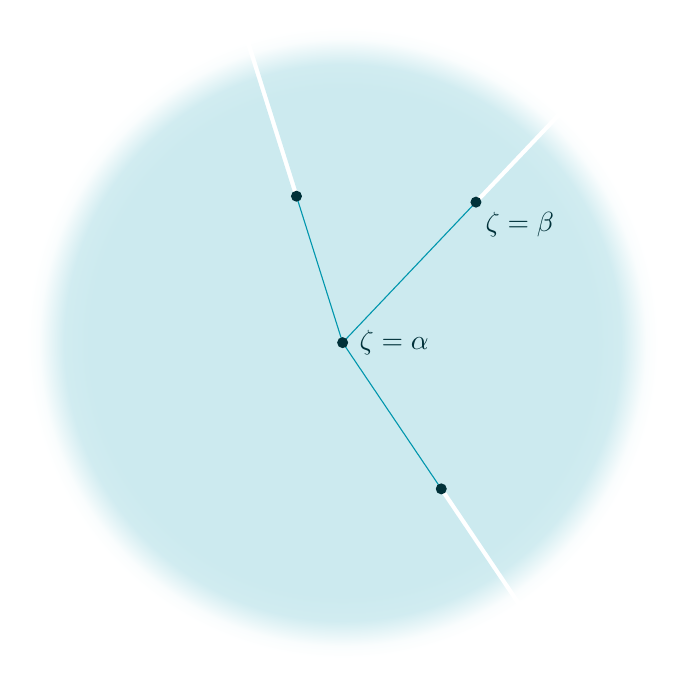
\begin{tikzpicture}
\newcommand{\spill}{4}
\newcommand{\slitsize}{0.4}
\fill[ietcoast!20, bezier bounding box, path fading=radial edge]
  (-\spill, -\spill) (\spill, \spill)
  (0, 0) -- (180:\spill)
  arc (180:107.5+\slitsize:\spill) -- (107.5+\spill/1.95*\slitsize:1.95) -- (107.5-\spill/1.95*\slitsize:1.95) -- (107.5-\slitsize:\spill)
  arc (107.5-\slitsize:46.5+\slitsize:\spill) -- (46.5+\spill/2.46*\slitsize:2.46) -- (46.5-\spill/2.46*\slitsize:2.46) -- (46.5-\slitsize:\spill)
  arc (46.5-\slitsize:-56+\slitsize:\spill) -- (-56+\spill/2.24*\slitsize:2.24) -- (-56-\spill/2.24*\slitsize:2.24) -- (-56-\slitsize:\spill)
  arc (-56-\slitsize:-180:\spill) -- (0, 0);
\node[ietcoast!33!black, anchor=north west] at (46.5:2.46) {$\zeta = \beta$};
\foreach \p in {(107.5:1.95), (46.5:2.46), (-56:2.24)} {
  \draw[ietcoast] \p -- (0,0);
  \fill[ietcoast!33!black] \p circle (0.7mm);
}
\fill[ietcoast!33!black] circle (0.7mm) node[anchor=180, outer sep=1mm] {$\zeta = \alpha$};
\end{tikzpicture}
\captionof{figure}{The domain $\Omega_\alpha$}\label{Fig:slit domain}
\end{center}
\begin{revised}Initially, the function $\int_{\mathcal{C}_a(\zeta)} \nu$ is only defined for $\zeta$ on the ray $[\alpha, \infty)$, but it can be analytically continued to points off the ray by homotopy of the path $\mathcal{C}_a(\zeta)$. Since $\nu$ is holomorphic, the only way for $\int_{\mathcal{C}^\theta_a(\zeta)} \nu$ to become singular is for something to go wrong with the hotmotopy of $\mathcal{C}_a(\zeta)$, which can only happen at the critical values of $f$. Therefore, $\mathcal{C}_a(\zeta)$ is endlessly analytically continuable away from the critical values of $f$. Resurgent functions have resurgent derivatives \begin{todo}[check]\end{todo}, so $\iota_\alpha$ is resurgent too.\end{revised}
\begin{old}\par
\begin{todo}[Incorporate this additional work]\end{todo} We will calculate the jump of $\int_{\mathcal{C}_a^\theta(\zeta)}\nu$ across the cut starting at $\zeta = \beta$. Write $\beta$ as $\alpha + re^{i\theta_\beta}$, and let $\beta^+$ and $\beta^-$ be the values we get by infinitesimally increasing or decreasing $\theta_\beta$. The jump is then given by \[\int_{\mathcal{C}_a^\theta(\beta^+)} \nu - \int_{\mathcal{C}_a^\theta(\beta^-)} \nu\] 
and it turns out to be proportional to $\series{\phi}_\beta$, namely to the germ of analytic functions at $\zeta_\alpha=\beta$. %We will see an example of this behaviour in Appendix~\ref{apx:eye-res-airy}. 

\begin{todo}[This paragraph is marked as revised]\end{todo} Initially, the function $\int_{\mathcal{C}^\theta_a(\zeta)} \nu$ is only defined for $\zeta$ on the ray $[\alpha, \infty)$, but it can be analytically continued to points off the ray by homotopy of the path $\mathcal{C}^\theta_a(\zeta)$. Since $\nu$ is holomorphic, the only way for $\int_{\mathcal{C}^\theta_a(\zeta)} \nu$ to be singular is for something to go wrong with the hotmotopy of $\mathcal{C}^\theta_a(\zeta)$. At a critical point of $f$, the ends of the homotoped path $\mathcal{C}^\theta_a(\zeta)$ come together, telling us that \begin{todo}[\textbf{A} \textbf{V} \ldots]\end{todo}
\end{old}
\end{remark}
\begin{todo}
\begin{corollary}\label{simple-res-thimble}
If $f$ and $\nu$ are polynomials, the function ${\phi}=\fracderiv{-1/2}{\zeta}{\alpha}\iota$ defined in Remark~\ref{rmk:1/2-deriv} has simple resurgent singularities at $\zeta=\beta$, for all $\beta$ roots of $P$ such that $\beta\neq\alpha$.  
\end{corollary}
\begin{proof}
Recall ${\phi}_\alpha$ is the sum of the Borel transform of $z^{1/2}\series{I}_j$, namely 
\[\hat{\phi}_j(\zeta)=\fracderiv{1/2}{\zeta}{\alpha_j}\hat{\iota}_j=\int_{\alpha_j}^\zeta(\zeta-s)^{-3/2}\hat{\iota}_j(s)\, ds\]
Then by Pham's result (see \eqref{rmk:Pham formula}) we know 
\[\hat{\iota}_j(\zeta_j)=\frac{(-\zeta_j)^{-1/2}}{2\pi i\Gamma(-\tfrac{1}{2})}\sum_{k=0}^\infty c_k (-\zeta_j)^{-k} + \text{ hol. funct. }\]
hence 
\[\hat{\iota}_j(\zeta)=\int_{\alpha_j}^\zeta(\zeta-s)^{-3/2}\frac{(-s+\alpha_j)^{-1/2}}{2\pi i\Gamma(-\tfrac{1}{2})}\sum_{k=0}^\infty c_k (-s+\alpha_j)^{-k} \, ds + \text{ hol. funct. }\]
\end{proof}
\end{todo}
\begin{remark}\label{rmk:Pham formula}
When $f$ and $\nu$ are polynomials and $X$ is $N$-dimensional, a result of Pham \cite[Equation 2.4, II partie]{pham} gives us an explicit expression for the singularity of the function $\iota_a$ from Lemma~\ref{lem:thimble_proj_formula-proof}. For some coefficients $c_k$ which depend on $f$, $\nu$, and the thimble $\mathcal{C}_a^\theta$, we have
\begin{equation}\label{eqn:Pham}
\iota_a \in (-1)^{\frac{N(N-1)}{2}}  \sum_{k=0}^\infty c_k\, \delta_{\zeta, \alpha}^{(-N/2 - k)} + \mathcal{O}_{\zeta = \alpha},
\end{equation}
where the singularities
\begin{equation*}
\delta_{\zeta,\alpha}^{(-\ell)}:=\begin{cases}
\displaystyle\frac{\zeta_\alpha^{\ell-1}}{-2\pi i(\ell-1)!}\log(\zeta_\alpha)+ \mathcal{O}_{\zeta = \alpha} & \text{ if } \ell\in\mathbb{N}^*\\
& \\
\displaystyle\frac{(-\zeta_\alpha)^{\ell-1}}{2\pi i\, \Gamma(-\ell)}+ \mathcal{O}_{\zeta = \alpha} & \text{ if } \ell\notin \mathbb{N}^* \,.
\end{cases}
\end{equation*}
can be seen as fractional derivatives of the Dirac delta distribution. In particular, if $N=1$, the inverse Laplace transform of the function $I_a$ from Equation~\eqref{exp-int} has a singularity of the form $\zeta_\alpha^{1/2}$, as we compute explicitly in the proof of Theorem~\ref{thm:maxim-proof}. %as computed in Remark~\ref{rmk:1/2-deriv} the inverse Laplace tranform of $z^{-1/2} I$ is the $1/2$-derivative of ${\iota}$, hence it has \textcolor{orange}{simple singularities (see Corollary~\ref{simple-res-thimble})}. \textcolor{magenta}{We expect this result to hold beyond the polynomial case.} We also expect that equation \eqref{eqn:formula-proof} can be generalized to the $N$-dimensional case replacing the $1/2$-derivative with the $N/2$ one. 
\end{remark}
\section{Examples}\label{sec:examples}
%
\subsection{Airy}\label{sec:airy}
%
The Airy equation is
\begin{equation}\label{eqn:airy}
\left[\big(\tfrac{\partial}{\partial y}\big)^2 - y\right] \Phi = 0.
\end{equation}
One solution is given by the Airy function,
\[ \Ai(y) = \frac{1}{2\pi i} \int_\gamma \exp\left(\tfrac{1}{3}t^3 - yt\right)\,dt, \]
where $\gamma$ is a path that comes from $\infty$ at $-60^\circ$ and returns to $\infty$ at $60^\circ$.

With the substitution $t = 2uy^{1/2}$, we can rewrite the Airy integral as
\begin{equation}\label{eqn:airy-distillation}
\Ai(y) = y^{1/2}\;\frac{1}{\pi i} \int_{\mathcal{C}^\theta_1} \exp\left[\tfrac{2}{3}y^{3/2} \left(4u^3 - 3u\right)\right]\,du,
\end{equation}
where $\mathcal{C}^\theta_1$ is the contour that passes through the point $u = \tfrac{1}{2}$ and projects to the ray $\mathcal{J}^\theta_{\zeta, 1}$ under the mapping $-\zeta = 4u^3 - 3u$.
\begin{center}
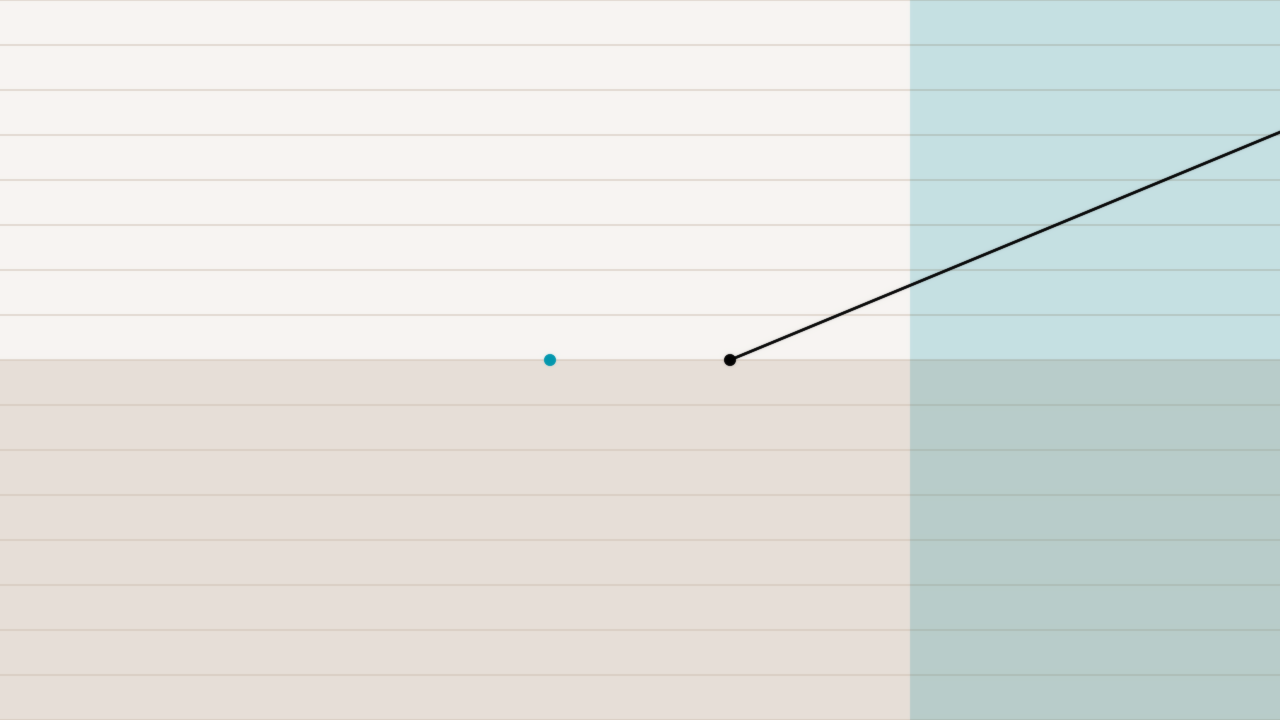
\includegraphics[width=6.5cm]{figures/ray_1_ge3.png}
\hspace{0.5cm}
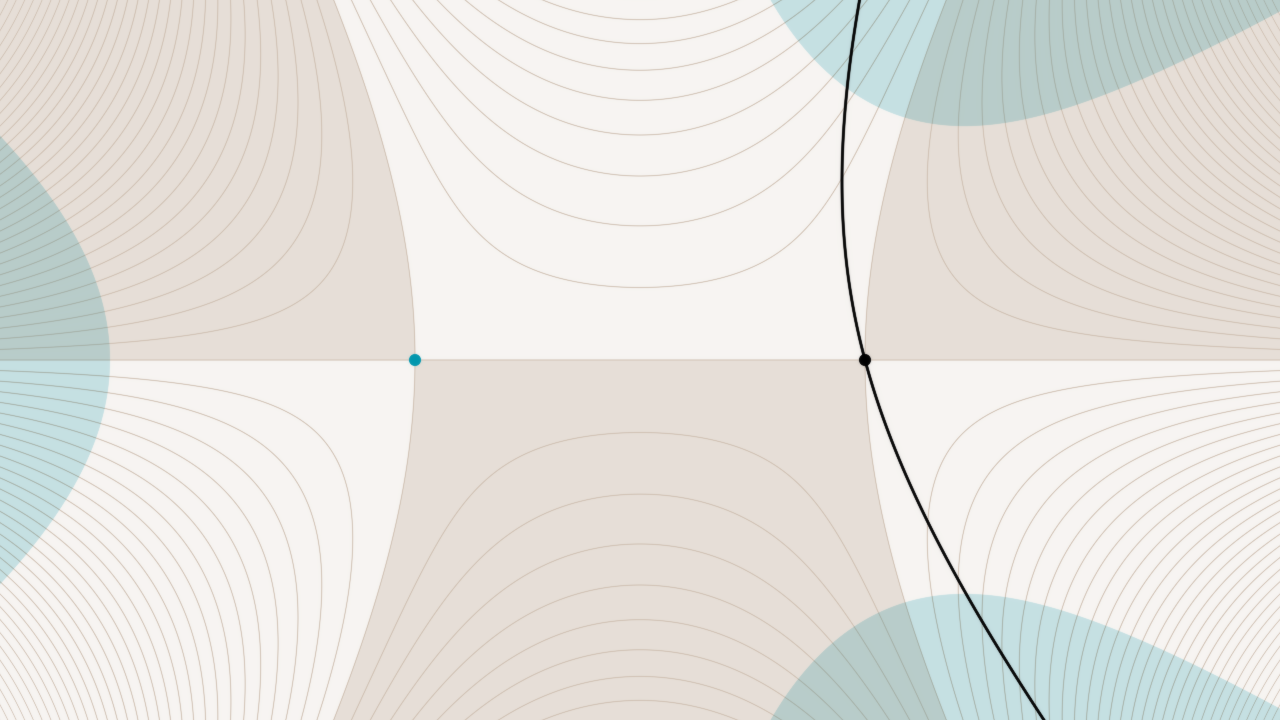
\includegraphics[width=6.5cm]{figures/thimble-n3_1.png}
\captionof{figure}{The ray $\mathcal{J}^{\pi/8}_{\zeta, 1}$ in the $\zeta$ plane and its preimage $\mathcal{C}^{\pi/8}_1$ in the $u$ plane. The upper and lower halves of the $\zeta$ plane are colored light and dark, so their preimages form a checker pattern on the $u$ plane. The region $\Re(\zeta) > 3$ and its preimage in the $u$ plane are shaded.}\label{fig:path_Airy}
\end{center}

Note that $4u^3 - 3u$ is the third Chebyshev polynomial. By considering other Chebyshev polynomials, we can situate the Airy function within the family of {\em Airy-Lucas functions}. Treating these functions as a family adds more insight than complexity, so we will go straight to the general case. However, since the Airy function is a classic example in the study of Borel summation and resurgence, it may be worth seeing on its own. In Appendix~\ref{airy-appendix}, we give a detailed treatment of the Airy function, specializing our arguments from the general case.

\subsection{Airy--Lucas}\label{example_AL}
The Airy-Lucas equation is
\begin{equation}\label{eqn:airy-lucas}
\left[\big(\tfrac{\partial}{\partial y}\big)^2 - (m-1) y^{-1} \tfrac{\partial}{\partial y} - y^{n-2}\right] \Phi = 0
\end{equation}
with $n \in \{3, 4, 5, \ldots\}$ and $m \in \{1, 2, \ldots, n-1\}$. A few solutions, indexed by $j \in \{1, \ldots, n-1\}$, are given by the Airy-Lucas functions~\cite[equation~3.6]{charbonnier22}
\begin{equation}\label{integral:AL}
\widehat{\Ai}^{(j)}_{n, m-1}(y) = \left\{\begin{array}{ll}i & j \text{ odd} \\ 1 & j \text{ even}\end{array}\right\} \frac{y^{m/2}}{\pi} \int_{\mathcal{C}^\theta_j} \exp\left[\tfrac{2}{n} y^{n/2}\,T_n(u)\right]\,U_{m-1}(u)\,du,
\end{equation}
where $\mathcal{C}^\theta_j$ is the contour that passes through the point $u = \cos\big(\tfrac{j}{n}\pi\big)$ and projects to the ray $\mathcal{J}^\theta_{\zeta, \pm 1}$ under the mapping $-\zeta = T_n(u)$. The ray starts at the critical value $1$ when $j$ is odd, and $-1$ when $j$ is even. To ensure that the integral converges, $\theta$ should be near $-\tfrac{n}{2} \arg(y)$.
\begin{center}
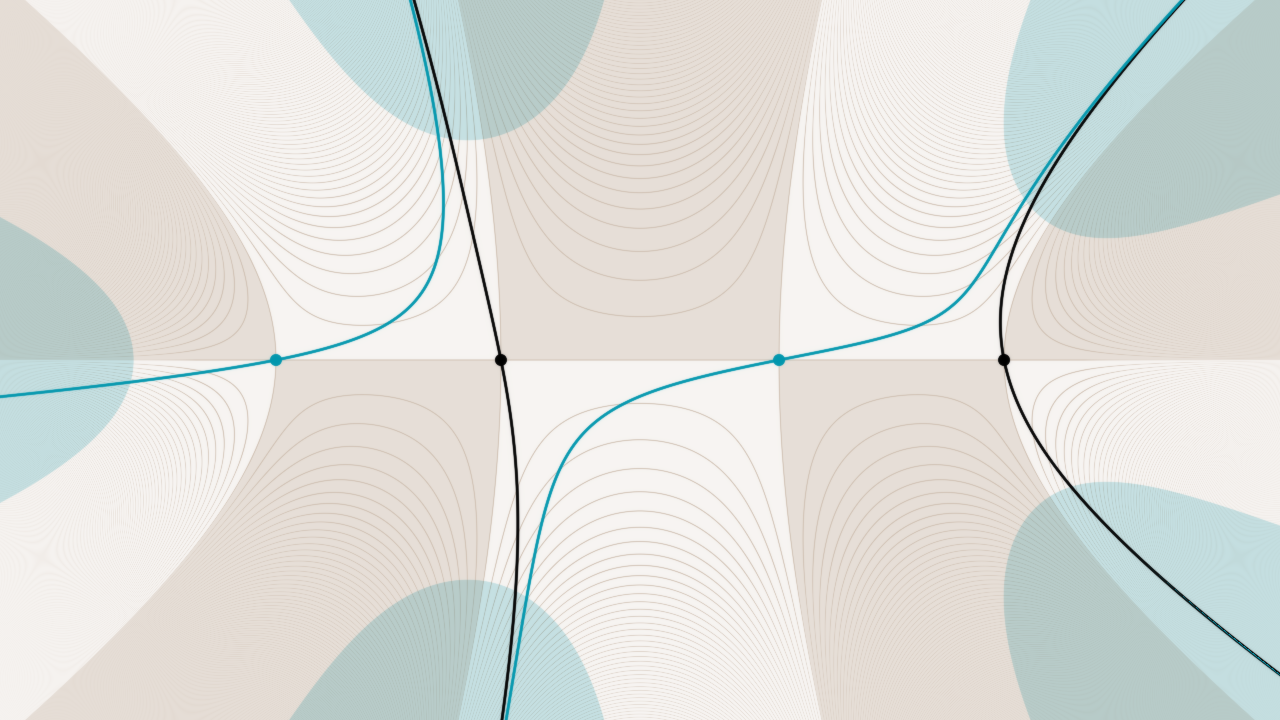
\includegraphics[width=10cm]{figures/thimbles-n5.png}
\captionof{figure}{The integration contours $\mathcal{C}^{\pi/8}_1, \ldots, \mathcal{C}^{\pi/8}_4$ for the Airy--Lucas functions with $n=5$. The dark and light thimbles are the preimages of the rays $\mathcal{J}^{\pi/8}_{\zeta, 1}$ and $\mathcal{J}^{\pi/8}_{\zeta, -1}$, respectively.}\label{fig:thimble_n_5}
\end{center}
\subsubsection{Rewriting as a modified Bessel $\frac{m}{n}$ equation}
We can distill the most interesting parts of the Airy-Lucas function by writing
\[ \widehat{\Ai}^{(j)}_{n, m-1}(y) = \frac{2 \sinh\big(\tfrac{m}{n}\,i\pi\big)}{n\pi} \left\{\begin{array}{ll}i & j \text{ odd} \\ 1 & j \text{ even}\end{array}\right\}\,y^{{m/2}}\,K^{(j)}_{m/n}\big(\tfrac{2}{n} y^{n/2}\big), \]
where
\begin{equation}\label{integral:mod-bessel-rational-AL}
K^{(j)}_{m/n}(z) = \frac{n}{2 \sinh\big(\tfrac{m}{n}\,i\pi\big)}\int_{\mathcal{C}^\theta_j} \exp\left[z T_n(u)\right]\,U_{m-1}(u)\,du.
\end{equation}
Saying that $\widehat{\Ai}^{(j)}_{n, m-1}$ satisfies the Airy-Lucas equation is equivalent to saying that $K^{(j)}_{m/n}$ satisfies the modified Bessel equation with parameter $\frac{m}{n}$:
\begin{equation}\label{eqn:mod-bessel-AL}
\left[z^2 \big(\tfrac{\partial}{\partial z}\big)^2 + z \tfrac{\partial}{\partial z} - \big[\big(\tfrac{m}{n} \big)^2 + z^2\big]\right] \Phi = 0.
\end{equation}
%%[DROPPED] In fact, as we will see in Section~\ref{contour-argument-AL}, $K$ is the modified Bessel function $K_{{m/n}}$.
Let us put equation~\eqref{eqn:mod-bessel-AL} in the form $\mathcal{P}\Phi=0$ with $\mathcal{P}$ as in equation~\eqref{eqn:operator-P}:
\begin{equation}\label{eqn:reg-mod-bessel-AL}
\left[ \big[ \big(\tfrac{\partial}{\partial z}\big)^2 - 1 \big] + z^{-1} \tfrac{\partial}{\partial z} - \big({\tfrac{m}{n}}\big)^2 z^{-2} \right] \Phi = 0.
\end{equation}
%
\subsubsection{Asymptotic analysis}\label{sec:asympt-AL}
%
From the work of Poincar\'{e} and the Ramis Index Theorem, as discussed at the beginning of Section~\ref{sec:new-summability-proof}, we know that equation~\eqref{eqn:reg-mod-bessel-AL} has a frame of formal $1$-Gevrey trans-monomial solutions
\[ \{ e^{-\alpha z} z^{-\tau_\alpha}\,\series{W}_\alpha \mid \alpha^2 - 1 = 0 \}, \]
where $\tau_\alpha = 1/2$ and $\series{W}_\alpha\in\C\llbracket z^{-1} \rrbracket_1$. From \cite[Equations 10.40.2 and 10.17.1]{dlmf}, we learn that $K_{m/n} \sim \left(\tfrac{\pi}{2}\right)^{1/2} e^{-z} z^{-1/2}\,\series{W}_1$, with
\begin{equation}\label{bessel-asymp-AL}
\series{W}_1 = 1 - \frac{\left(\tfrac{1}{2}-\tfrac{m}{n}\right)_1 \left(\tfrac{1}{2}+\frac{m}{n}\right)_1}{2^1 \cdot 1!}\;z^{-1} + \frac{\left(\tfrac{1}{2}-\tfrac{m}{n}\right)_2 \left(\tfrac{1}{2}+\tfrac{m}{n}\right)_2}{2^2 \cdot 2!}\;z^{-2} - \frac{\left(\tfrac{1}{2}+\tfrac{m}{n}\right)_3 \left(\tfrac{1}{2}+\tfrac{m}{n}\right)_3}{2^3 \cdot 3!}\;z^{-3} + \ldots
\end{equation}
%
The holomorphic analysis in Section~\ref{big-idea} will give us holomorphic solutions
\[ \{ e^{-\alpha z} z^{-\tau_\alpha}\,W_\alpha \mid \alpha^2 - 1 = 0 \}, \]
which seem analogous to the trans-monomials above. Borel summation makes the analogy precise. We will see in Section~\ref{bessel-regularity-AL} that each $z^{-\tau_\alpha}\,W_\alpha$ is proportional to the Borel sum of $z^{-\tau_\alpha}\,\series{W}_\alpha$, as required by Theorem~\ref{thm:summability_ODE}.
%
\subsubsection{The big idea}\label{big-idea}
%
We are going to look for functions $v_\alpha$ whose Laplace transforms $\laplace_{\zeta, \alpha} v_\alpha$ satisfy equation~\eqref{eqn:reg-mod-bessel-AL}. We will succeed when $\alpha^2 - 1 = 0$, and we will see that $K_{m/n}$ is a scalar multiple of $\laplace_{\zeta, 1} v_1$.

By the properties of the Laplace transform laid out in Proposition~\ref{prop:L-int-op}, a function $\laplace_{\zeta, \alpha} v$ satisfies the differential equation~\eqref{eqn:reg-mod-bessel-AL} if and only if $v$ satisfies the integral equation
\begin{equation}\label{int-eq:spatial-mod-bessel-AL}
\left[ \big[ \zeta^2 - 1 \big] - \fracderiv{-1}{\zeta}{\alpha} \circ \zeta - \big(\tfrac{m}{n}\big)^2 \fracderiv{-2}{\zeta}{\alpha} \right] v = 0.
\end{equation}
It is tempting to differentiate both sides of this equation until we get
\begin{equation}\label{diff-eq:spatial-mod-bessel-AL}
\left[ \big(\tfrac{\partial}{\partial \zeta}\big)^2 \circ \big[ \zeta^2 - 1 \big] - \tfrac{\partial}{\partial \zeta} \circ \zeta - \big(\tfrac{m}{n}\big)^2 \right] v = 0,
\end{equation}
which is easier to solve. Unfortunately, an analytic solution of equation~\eqref{diff-eq:spatial-mod-bessel-AL} will not satisfy equation~\eqref{int-eq:spatial-mod-bessel-AL} in general. However, as we show in Appendix~\ref{shifting}, a solution of equation~\eqref{diff-eq:spatial-mod-bessel-AL} {\em will} satisfy equation~\eqref{int-eq:spatial-mod-bessel-AL} if it belongs to $(\zeta - \alpha)^\sigma \mathcal{O}_{\zeta = \alpha}$ for some $\sigma \in (-1, 0)$.

This is good news, because equation~\eqref{diff-eq:spatial-mod-bessel-AL} has a regular singularity at each root of $\zeta^2 - 1$, and the Frobenius method often gives a solution of the desired kind at each regular singular point. We can see the regular singularities by rewriting equation~\eqref{diff-eq:spatial-mod-bessel-AL} as follows:
\[ \left[ (\zeta^2 - 1) \big(\tfrac{\partial}{\partial \zeta}\big)^2 + 3\zeta \tfrac{\partial}{\partial \zeta} + \big[ 1 - \big(\tfrac{m}{n}\big)^2 \big] \right] v = 0. \]

In Sections \ref{pos-root-AL}\,--\,\ref{neg-root-AL}, we will see this approach succeed. For each root $\alpha$, we will find a solution $v_\alpha$ of equation~\eqref{diff-eq:spatial-mod-bessel-AL} that belongs to $(\zeta - \alpha)^{\tau_\alpha-1}\,\mathcal{O}_{\zeta = \alpha}$ for some constant $\tau_\alpha \in (0, 1)$. We will express $v_\alpha$ explicitly enough to see that it extends to a function in $\singexpalg{\tau_\alpha-1}(\Omega_\alpha)$ on any sector $\Omega_\alpha$ that has its tip at $\zeta = \alpha$ and does not touch the other roots (see Figure~\ref{fig:sectorial_domain--with roots P}). We will also be able to see that $v_\alpha$ is uniformly of exponential type $\Lambda$ for any $\Lambda > 0$. It follows by Proposition~\ref{prop:laplace-cont} that for any ray $\mathcal{J}^\theta_{\zeta, \alpha}$ in $\Omega_\alpha$, the Laplace transform $\laplace^\theta_{\zeta, \alpha} v_\alpha$ is a well-defined element of $\dualsingexp{-\tau_\alpha}(\widehat{\Omega}_\alpha^\Lambda)$ that satisfies equation~\eqref{eqn:reg-mod-bessel-AL}. Using the technique from the proof of Lemma~\ref{lem:laplace-bridge}, we can see more precisely that $\laplace^\theta_{\zeta, \alpha} v_\alpha$ belongs to
\[ cz^{-\tau_\alpha} + \dualsingexp{-\tau_\alpha-1}(\widehat{\Omega}_\alpha^\Lambda) \]
for some non-zero constant $c$, confirming the existence part of Theorem~\ref{re:thm:exist_uniq_ODE}.

We know from Section~\ref{sec:change-translation} that
\[ \laplace^\theta_{\zeta, \alpha} v_\alpha = e^{-\alpha z} V_\alpha \]
for $V_\alpha \defeq \laplace^\theta_{\zeta_\alpha, 0} v_\alpha$ and $\zeta = \alpha + \zeta_\alpha$. Observing that multiplication by $z^{-\tau_\alpha}$ gives an isometry $\dualsingexp{0}(\widehat{\Omega}_\alpha^\Lambda) \to \dualsingexp{-\tau_\alpha}(\widehat{\Omega}_\alpha^\Lambda)$, we can do the further decomposition
\[ \laplace_{\zeta, \alpha} v_\alpha = e^{-\alpha z} z^{-\tau_\alpha} W_\alpha, \]
where $W_\alpha$ is a bounded holomorphic function on $\widehat{\Omega}_\alpha^\Lambda$.
%
\subsubsection{Focus on $\zeta = 1$}\label{pos-root-AL}
%
Let us find a germ in $(\zeta-1)^{\tau_1-1}\,\mathcal{O}_{\zeta=1}$, for some $\tau_1 \in (0, 1)$, that satisfies equation~\eqref{diff-eq:spatial-mod-bessel-AL}. Define a new coordinate $\zeta_1$ on $\C$ so that $\zeta = 1 + \zeta_1$. In this coordinate, equation~\eqref{diff-eq:spatial-mod-bessel-AL} looks like
\begin{equation}\label{diff-eq:spatial-mod-bessel-pos-AL}
\left[\zeta_1(2 + \zeta_1) \big(\tfrac{\partial}{\partial \zeta_1}\big)^2 + 3(1 + \zeta_1) \tfrac{\partial}{\partial \zeta_1} + \big[1 - \big(\tfrac{m}{n}\big)^2\big]\right] v = 0.
\end{equation}
With another change of coordinate, given by $\zeta_1 = -2\xi_1$, we can rewrite equation~\eqref{diff-eq:spatial-mod-bessel-AL} as the hypergeometric equation
\begin{equation}\label{diff-eq:hypergeom-pos-AL}
\left[\xi_1 (1 - \xi_1) \big(\tfrac{\partial}{\partial \xi_1}\big)^2 + 3(\tfrac{1}{2} - \xi_1) \tfrac{\partial}{\partial \xi_1} - \big[1 - \big(\tfrac{m}{n}\big)^2\big]\right] v = 0.
\end{equation}
Looking through the twenty-four expressions for Kummer's six solutions, we find one \cite[formula~15.10.12]{dlmf} that represents a germ in $\xi_1^{-1/2}\,\mathcal{O}_{\xi_1=0}$:
\begin{alignat*}{2}
v_1 &=\;& \hphantom{-i\sqrt{2}}\,\xi_1^{-1/2} & {}_2F_1\big(\tfrac{1}{2}-\tfrac{m}{n}, \tfrac{1}{2}+\tfrac{m}{n}; \tfrac{1}{2}; \xi_1\big) \\[1mm]
&=\;& -i\sqrt{2}\,\zeta_1^{-1/2} & {}_2F_1\big(\tfrac{1}{2}-\tfrac{m}{n}, \tfrac{1}{2}+\tfrac{m}{n}; \tfrac{1}{2}; -\tfrac{1}{2}\zeta_1\big)
\end{alignat*}

From the expression above, we can see that $v_1$ has only two singularities in the complex plane: one at $\zeta_1 = 0$ from the factor of $\zeta_1^{-1/2}$, and one at $\zeta_1 = -2$ from the hypergeometric function. Therefore, $v_1$ is holomorphic throughout the sector $\Omega_1 = \C \smallsetminus \mathcal{J}^\pi_{\zeta_1, 0}$. Since $v_1$ has a power law singularity at $\infty$, it is uniformly of exponential type $\Lambda$ for any $\Lambda > 0$. Therefore, it belongs to the space $\singexp{-1/2}{\Lambda}(\Omega_1)$ for all $\Lambda > 0$. By thinking about its shifted Taylor expansion around $\zeta_1 = 0$, we can see more precisely that $v_1$ belongs to
\[ -i\sqrt{2}\,\zeta_1^{-1/2} + \singexp{1/2}{\Lambda}(\Omega_1) \]
for all $\Lambda > 0$. As discussed in Section~\ref{big-idea}, we conclude that $v_1$ has a well-defined Laplace transform along any ray from $\zeta = 1$ except the one going directly left. Its Laplace transform can be written as
\[ \laplace^\theta_{\zeta, 1} v_1 = e^{-z} z^{-1/2}\,W_1, \]
where $W_1$ is a holomorphic function on $z \notin (-\infty, 0]$ which is bounded outside any constant-radius neighborhood of $z \in (-\infty, 0]$.
%
\subsubsection{Focus on $\zeta = -1$}\label{neg-root-AL}
%
Let us find a germ in $(\zeta+1)^{\tau_{-1}-1}\,\mathcal{O}_{\zeta=-1}$, for some $\tau_{-1} \in (0, 1)$, that satisfies equation~\eqref{diff-eq:spatial-mod-bessel-AL}. In the rescaled coordinate from Section~\ref{pos-root-AL}, this is the point $\xi_1 = 1$. Looking again through Kummer's table of solutions, we find another expression \cite[formula~15.10.14]{dlmf} that represents a germ in $(1-\xi_1)^{-1/2}\,\mathcal{O}_{\xi_1=1}$:
\begin{alignat*}{2}
v_{-1} &=\;& (1-\xi_1)^{-1/2} &\;{}_2F_1\big(\tfrac{1}{2}-\tfrac{m}{n}, \tfrac{1}{2}+\tfrac{m}{n}; \tfrac{1}{2}; 1-\xi_1\big) \\[1mm]
&=\;& \sqrt{2}\,\zeta_{-1}^{-1/2} &\;{}_2F_1\big(\tfrac{1}{2}-\tfrac{m}{n}, \tfrac{1}{2}+\tfrac{m}{n}; \tfrac{1}{2}; \tfrac{1}{2}\zeta_{-1}\big),
\end{alignat*}
where $\zeta_{-1}$ is the coordinate with $\zeta = -1 + \zeta_{-1}$. By the same reasoning as before, $v_{-1}$ is holomorphic throughout the sector $\Omega_{-1} = \C \smallsetminus \mathcal{J}^0_{\zeta_{-1}, 0}$, and it belongs to the space
\[ \sqrt{2}\,\zeta_{-1}^{-1/2} + \singexp{1/2}{\Lambda}(\Omega_1) \]
for all $\Lambda > 0$. It has a well-defined Laplace transform along any ray from $\zeta = -1$ except the one going directly right, and its Laplace transform can be written as
\[ \laplace^\theta_{\zeta, -1} v_1 = e^z z^{-1/2}\,W_{-1}, \]
where $W_{-1}$ is a holomorphic function $z \notin [0, \infty)$ which is bounded outside any constant-radius neighborhood of $z \in [0, \infty)$.

%%From the argument in Section~\ref{big-idea}, we know that $\laplace_{\zeta, -1} v_{-1}$ satisfies equation~\eqref{eqn:mod-bessel-AL}, and can be written as $e^z V_{-1}$, where $V_{-1} = \laplace_{\zeta_{-1}, 0} v_{-1}$. Since $v_{-1}$, like our other solution, \textcolor{magenta}{has order $-1/2$}, the same decomposition $V_{-1} = z^{-1/2} W_{-1}$ makes $W_{-1}$ asymptotic to a scalar multiple of $1+O(z^{-1})$ at $z = \infty$.

In this example, $v_1$ and $v_{-1}$ happen to be related by a symmetry: the M\"{o}bius transformation that pulls $\zeta$ back to $-\zeta$. Kummer's solutions typically come from six different hypergeometric equations, which are related by the M\"{o}bius transformations that permute their singularities. In our case, though, exchanging $1$ with $-1$ keeps equation~\eqref{diff-eq:spatial-mod-bessel-AL} the same.
\subsubsection{Abstract argument for Borel regularity}\label{bessel-regularity-AL}
The analysis in Sections~\ref{big-idea}\;--\;\ref{neg-root-AL} picks out a frame in the space of analytic solutions of~\eqref{eqn:reg-mod-bessel-AL}. The frame is generated by solutions of the form $\laplace_{\zeta, 1} v_1$ and $\laplace_{\zeta, -1} v_{-1}$, with $v_\alpha \in \singexpalg{-1/2}(\Omega_\alpha)$.

The Poincar\'{e} algorithm, as discussed in Section~\ref{sec:asympt-AL} picks out a frame in a space of formal solutions of equation~\eqref{eqn:reg-mod-bessel-AL}. The frame is generated by $1$-Gevrey trans-monomial solutions of the form $e^{-z} z^{-1/2}\,\tilde{W}_1$ and $e^z z^{-1/2}\,\tilde{W}_{-1}$, with $\tilde{W}_j \in \C\llbracket z^{-1} \rrbracket_1$. Reprising the proof of Theorem~\ref{thm:summability_ODE}, we will show that these solutions are Borel summable, and their Borel sums generate the same frame as $\laplace_{\zeta, 1} v_1$ and $\laplace_{\zeta, -1} v_{-1}$.

The Borel transform $\borel_\zeta$ maps $e^{-\alpha z} z^{-1/2}\,\C\llbracket z^{-1} \rrbracket_1$ into $\zeta_\alpha^{-1/2}\,\C\{\zeta_\alpha\}$, as discussed in Sections \ref{sec:action_transseries} and \ref{sec:new-summability-proof}. In particular, it sends each Poincar\'{e} solution $e^{-\alpha z} z^{-1/2}\,\series{W}_\alpha$ to a convergent series $\series{v}_\alpha \in \zeta_\alpha^{-1/2}\,\C\{\zeta_\alpha\}$. Make a bounded sector $\Omega'_\alpha$ by intersecting $\Omega_\alpha$ with a disk around $\zeta_\alpha = 0$ whose radius is smaller than the radius of convergence of $\series{v}_\alpha$. On $\Omega'_\alpha$, the sum $\hat{v}_\alpha$ of $\series{v}_\alpha$ can be bounded by a shifted geometric series, showing that $\zeta_\alpha^{1/2} \hat{v}_\alpha$ is bounded by a constant. Therefore, $\hat{v}_\alpha$ belongs to $\singexpalg{-1/2}(\Omega'_\alpha)$.

The Borel transform
\[ \borel_\zeta \maps e^{-\alpha z} z^{-1/2}\,\C\llbracket z^{-1} \rrbracket_1 \to \zeta_\alpha^{-1/2}\,\C\{\zeta_\alpha\} \]
also turns formal trans-monomial solutions of equation~\eqref{eqn:reg-mod-bessel-AL} into formal power series solutions of equation~\eqref{int-eq:spatial-mod-bessel-AL}. Thus, by the dominated convergence theorem, $\hat{v}_\alpha$ is an analytic solution of equation~\eqref{int-eq:spatial-mod-bessel-AL} on $\Omega'_\alpha$. The uniqueness part of Theorem~4 from \cite{reg-sing-volterra} then shows that $\hat{v}_\alpha$ must be a scalar multiple of the solution $v_\alpha$ we found in Sections \ref{big-idea}\;--\;\ref{neg-root-AL}. Since $v_\alpha$ belongs to $\singexpalg{-1/2}(\Omega_\alpha)$ for the full, unbounded sector $\Omega_\alpha$, it has a well-defined Laplace transform along any ray $\mathcal{J}^\theta_{\zeta, \alpha}$ in $\Omega_\alpha$. Therefore, the Poincar\'{e} solution $e^{-\alpha z} z^{-1/2}\,\series{W}_\alpha$ has a well-defined Borel sum along $\mathcal{J}^\theta_{\zeta, \alpha}$, which is a scalar multiple of $e^{-\alpha z} V_\alpha$. It follows, by Lemma~\ref{lem:laplace-bridge}, that $e^{-\alpha z} V_\alpha$ is Borel regular.
%
\subsubsection{Confirmation of Borel regularity}\label{confirmation-borel-regularity}
%
We can verify the conclusions of Section~\ref{bessel-regularity-AL} using our explicit expressions for the formal power series $\tilde{W}_\alpha$ and the functions $v_\alpha$. We found in Section~\ref{sec:asympt-AL} that
\begin{align*}
\tilde{W}_1 & = \sum_{k = 0}^{\infty} \frac{\left(\tfrac{1}{2}-\tfrac{m}{n}\right)_k \left(\tfrac{1}{2}+\tfrac{m}{n}\right)_k}{k!} \left(-\frac{1}{2}\right)^k z^{-k} \\
\tilde{W}_{-1} & = \sum_{k = 0}^{\infty} \frac{\left(\tfrac{1}{2}-\tfrac{m}{n}\right)_k \left(\tfrac{1}{2}+\tfrac{m}{n}\right)_k}{k!} \left(\frac{1}{2}\right)^k z^{-k}.
\end{align*}
Computing
\begin{align*}
\borel_\zeta \big[ e^{-z} z^{-1/2}\,\tilde{W}_1 \big] & = \borel_\zeta \left[ e^{-z} \sum_{k = 0}^{\infty} \frac{\left(\tfrac{1}{2}-\tfrac{m}{n}\right)_k \left(\tfrac{1}{2}+\tfrac{m}{n}\right)_k}{k!} \left(-\frac{1}{2}\right)^k z^{-k-\frac{1}{2}} \right] \\
& = \sum_{k = 0}^{\infty} \frac{\left(\tfrac{1}{2}-\tfrac{m}{n}\right)_k \left(\tfrac{1}{2}+\tfrac{m}{n}\right)_k}{k!} \left(-\frac{1}{2}\right)^k \frac{\zeta_1^{k-\frac{1}{2}}}{\Gamma\big(k+\frac{1}{2}\big)} \\
& = \sum_{k = 0}^{\infty} \frac{\left(\tfrac{1}{2}-\tfrac{m}{n}\right)_k \left(\tfrac{1}{2}+\tfrac{m}{n}\right)_k}{k!} \left(-\frac{1}{2}\right)^k \frac{\zeta_1^{k-\frac{1}{2}}}{\Gamma\big(\frac{1}{2}\big) \left(\frac{1}{2}\right)_k} \\
& = \frac{\zeta_1^{-\frac{1}{2}}}{\Gamma\big(\frac{1}{2}\big)} \sum_{k = 0}^{\infty} \frac{\left(\tfrac{1}{2}-\tfrac{m}{n}\right)_k \left(\tfrac{1}{2}+\tfrac{m}{n}\right)_k}{\left(\frac{1}{2}\right)_k} \left(-\frac{1}{2}\right)^k \frac{\zeta_1^k}{k!},
\end{align*}
we see that $\borel\big[ e^{-z} z^{-1/2}\,\tilde{W}_1 \big]$ sums to
\[ \tfrac{1}{\Gamma(1/2)}\,\zeta_1^{-1/2}\,{}_2F_1\big(\tfrac{1}{2}-\tfrac{m}{n}, \tfrac{1}{2}+\tfrac{m}{n}; \tfrac{1}{2}; -\tfrac{1}{2}\zeta_1\big). \]
Looking back at Section~\ref{pos-root-AL}, we recognize this as a scalar multiple of $v_1$.

Through a similar calculation, we see that $\borel\big[ e^z z^{-1/2}\,\tilde{W}_{-1} \big]$ sums to
\[ \tfrac{1}{\Gamma(1/2)}\,\zeta_{-1}^{-1/2}\,{}_2F_1\big(\tfrac{1}{2}-\tfrac{m}{n}, \tfrac{1}{2}+\tfrac{m}{n}; \tfrac{1}{2}; \tfrac{1}{2}\zeta_{-1}\big). \]
Looking back at Section~\ref{neg-root-AL}, we recognize this as a scalar multiple of $v_{-1}$.
%
\subsubsection{Thimble projection reasoning}\label{contour-argument-AL}
We can also study the Airy-Lucas functions by applying the thimble projection formula to integral~\eqref{integral:mod-bessel-rational-AL}, specializing the reasoning behind Lemma~\ref{lem:thimble_proj_formula-proof}. We recast integral~\eqref{integral:mod-bessel-rational-AL} into the $\zeta$ plane by setting $-\zeta = T_n(u)$, which implies that $-d\zeta = n U_{n-1}(u)\,du$. Recall from below equation~\eqref{integral:AL} that the integration contour $\mathcal{C}^\theta_j$ runs through the critical point $u = \cos\big(\tfrac{j}{n}\pi\big)$, with its direction determined by the parameter $\theta$. The critical point splits $\mathcal{C}^\theta_j$ into two pieces: the {\em incoming} branch, where the orientation of the thimble runs toward the critical point, and the {\em outgoing} branch, where the orientation points away. Recalling that $\mathcal{C}^\theta_j$ is a preimage of $\mathcal{J}^\theta_{\zeta, \mp 1}$, we get
\begin{align*}%%\label{integral:mod-bessel-rational-zeta}
K^{(j)}_{m/n}(z) & = \frac{n}{2 \sinh\big(\tfrac{m}{n}\,i\pi\big)} \int_{\mathcal{C}^\theta_j} \exp\left[z T_n(u)\right]\,U_{m-1}(u)\,du \\
& = -\frac{1}{2\sinh\big(\tfrac{m}{n}\,i\pi\big)} \left[ \int_{\mathcal{J}^\theta_{\zeta, \mp 1}} e^{-z\zeta}\,\frac{U_{m-1}(u_+)}{U_{n-1}(u_+)}\,d\zeta - \int_{\mathcal{J}^\theta_{\zeta, \mp 1}} e^{-z\zeta}\,\frac{U_{m-1}(u_-)}{U_{n-1}(u_-)}\,d\zeta \right],
\end{align*}
where $u_-$ and $u_+$ are the lifts to the incoming and outgoing branches of $\mathcal{C}^\theta_j$, respectively. \begin{todo}[Draw the thimble in the $u$ plane?]\end{todo}

Since the Chebyshev polynomial $T_n$ is defined by the identity $T_n(\cos(\phi)) = \cos(n\phi)$, we introduce a new variable $\phi$ with $u = \cos(\phi)$ and $-\zeta = \cos(n\phi)$. On the $\phi$ plane, which is an infinite branched cover of the $u$ plane, we can lift $\mathcal{C}^\theta_j$ to the path $\tfrac{j}{n}\pi + i\R$. The incoming and outgoing branches lift to $\tfrac{j}{n}\pi - i[0, \infty)$ and $\tfrac{j}{n}\pi + i[0, \infty)$, respectively. \begin{todo}[Draw the lifted thimble in the $\phi$ plane?]\end{todo}

We can now use identity~15.4.16 from \cite{dlmf} to write the integrand explicitly in terms of $\zeta$:
\begin{align*}
\frac{U_{m-1}(\cos(\phi))}{U_{n-1}(\cos(\phi))} &= \frac{\sin(m\phi)}{\sin(\phi)}\frac{\sin(\phi)}{\sin(n \phi)}\\
& = \frac{\sin(m\phi)}{\sin(n \phi)}\\
& = \frac{m}{n}\;{}_2F_1\left(\frac{1}{2} - \frac{m}{2n},\;\frac{1}{2} + \frac{m}{2n};\;\frac{3}{2};\;\sin(n \phi)^2\right) \\
& = \frac{m}{n}\;{}_2F_1\left(\frac{1}{2} - \frac{m}{2n},\;\frac{1}{2} + \frac{m}{2n};\;\frac{3}{2};\;1 - \zeta^2\right).
\end{align*}
Initially, we only know that this equation holds in the disk $|\phi| < \tfrac{\pi}{2n}$. However, observing that the left-hand side is meromorphic throughout the $\phi$ plane, we can deduce by analytic continuation that the equation holds throughout the $\phi$ plane.

Next, we simplify the integrand using identities 15.8.4 and 15.8.27\;--\;15.8.28 from \cite{dlmf}, which tell us that\begin{align*}
&{}_2F_1\left(\frac{1}{2} - \frac{m}{2n}, \frac{1}{2} + \frac{m}{2n}; \frac{3}{2}; 1 - \zeta^2\right) \\[3mm]
& =\; \hphantom{+} \frac{\pi}{\Gamma\left(1-\frac{m}{2n}\right) \Gamma\left(1 + \frac{m}{2n}\right)}\;{}_2F_1\left(\frac{1}{2} - \frac{m}{2n},\;\frac{1}{2} + \frac{m}{2n};\;\frac{1}{2};\;\zeta^2\right) \\
& \hphantom{=}\; - \frac{\pi \zeta}{\Gamma\left(\frac{1}{2} - \frac{m}{2n}\right) \Gamma\left(\frac{1}{2} + \frac{m}{2n}\right)}\;{}_2F_1\left(1 - \frac{m}{2n},\;1 + \frac{m}{2n};\;\frac{3}{2};\;\zeta^2\right) \\[3mm]
& =\; \hphantom{+ \frac{0}{0}}\;{}_2F_1\left(1 - \frac{m}{n},\;1 + \frac{m}{n};\;\frac{3}{2};\;\frac{1}{2} - \frac{\zeta}{2}\right) + \hphantom{\frac{0}{0}}\;{}_2F_1\left(1-\frac{m}{n},\;1 + \frac{m}{n};\;\frac{3}{2};\;\frac{1}{2} + \frac{\zeta}{2}\right) \\
& \hphantom{=}\; + \frac{1}{2}\;{}_2F_1\left(1-\frac{m}{n},\;1+\frac{m}{n};\;\frac{3}{2};\;\frac{1}{2} - \frac{\zeta}{2}\right) - \frac{1}{2}\;{}_2F_1\left(1-\frac{m}{n},\;1 + \frac{m}{n};\;\frac{3}{2};\;\frac{1}{2} + \frac{\zeta}{2}\right) \\[3mm]
& =\; \hphantom{+} \frac{3}{2}\;{}_2F_1\left(1 - \frac{m}{n},\;1 + \frac{m}{n};\;\frac{3}{2};\frac{1}{2} - \frac{\zeta}{2}\right) + \frac{1}{2}\;{}_2F_1\left(1 - \frac{m}{n},\;1 + \frac{m}{n};\;\frac{3}{2};\;\frac{1}{2} + \frac{\zeta}{2}\right)
\end{align*}
away from the line $\Re(\zeta) = 0$ and the rays $\mathcal{J}^0_{\zeta,1}$ and $\mathcal{J}^\pi_{\zeta,-1}$.

Returning to the projected thimble integral
\[ K^{(j)}_{m/n}(z) = -\frac{1}{2\sinh\big(\tfrac{m}{n}\,i\pi\big)} \int_{\mathcal{J}^\theta_{\zeta, \mp 1}} e^{-z\zeta} \left[ \frac{U_{m-1}(u_+)}{U_{n-1}(u_+)} - \frac{U_{m-1}(u_-)}{U_{n-1}(u_-)} \right] d\zeta, \]
we can see the integrand as the variation of the function
\[ \frac{U_{m-1}(\cos(\phi))}{U_{n-1}(\cos(\phi))} = \frac{3m}{2n}\;{}_2F_1\left(1 - \frac{m}{n},\;1 + \frac{m}{n};\;\frac{3}{2};\frac{1}{2} - \frac{\zeta}{2}\right) + \frac{m}{2n}\;{}_2F_1\left(1 - \frac{m}{n},\;1 + \frac{m}{n};\;\frac{3}{2};\;\frac{1}{2} + \frac{\zeta}{2}\right) \]
\begin{verify}
\begin{align*}
\frac{m}{2n}\,\frac{2\pi i}{\Gamma\big(1-\tfrac{m}{n}\big)\Gamma\big(1+\tfrac{m}{n}\big)} & = \frac{\pi i}{\Gamma\big(1-\tfrac{m}{n}\big)\Gamma\big(\tfrac{m}{n}\big)} \\
& = \pi i\,\frac{\sin\big(\pi\tfrac{m}{n}\big)}{\pi} \\
& = i \sin\big(\pi\tfrac{m}{n}\big) \\
&= \sinh\big(i\pi\tfrac{m}{n}\big)
\end{align*}
\end{verify}
across the branch cut $\mathcal{J}^\theta_{\zeta, \pm 1}$. When $j$ is odd, only the second term will contribute to the jump, because the first term is regular at $\zeta = 1$. Similarly, when $j$ is even, only the first term will contribute to the jump. We can write the jump explicitly using identity~15.2.3 from \cite{dlmf}. For odd $j$, we have
\[ K^{(j)}_{m/n}(z) = -\frac{1}{2} \int_{\mathcal{J}^\theta_{\zeta, 1}} e^{-z\zeta} \left(-\frac{1}{2}+\frac{\zeta}{2}\right)^{-1/2} {}_2F_1\left(\frac{1}{2} - \frac{m}{n},\;\frac{1}{2} + \frac{m}{n};\;\frac{1}{2};\;\frac{1}{2} - \frac{\zeta}{2}\right) d\zeta, \]
and for even $j$, we have
\[ K^{(j)}_{m/n}(z) = \frac{3}{2} \int_{\mathcal{J}^\theta_{\zeta, -1}} e^{-z\zeta} \left(-\frac{1}{2}-\frac{\zeta}{2}\right)^{-1/2} {}_2F_1\left(\frac{1}{2} - \frac{m}{n},\;\frac{1}{2} + \frac{m}{n};\;\frac{1}{2};\;\frac{1}{2} + \frac{\zeta}{2}\right) d\zeta. \]

Comparing the expressions above with the expressions for $v_{\pm 1}$ computed in Sections~\ref{pos-root-AL}\;--\;\ref{neg-root-AL}, we notice that
\[ K^{(j)}_{m/n}(z) = \begin{cases}
\hphantom{-}\frac{i}{2}\laplace_{\zeta, 1} v_1 & j \text{ odd} \\
-\frac{3i}{2}\laplace_{\zeta, -1} v_{-1} & j \text{ even}.
\end{cases} \]
\begin{verify}
\begin{align*}
\zeta & = 1 + \zeta_1 & -\zeta_1 & = 1 - \zeta \\
\zeta & = -1 + \zeta_{-1} & \zeta_{-1} & = 1 + \zeta
\end{align*}
\begin{align*}
\left(-\frac{1}{2}+\frac{\zeta}{2}\right)^{-1/2} & = \sqrt{2}\,\zeta_1^{-1/2} \\
\left(-\frac{1}{2}-\frac{\zeta}{2}\right)^{-1/2} & = \sqrt{2}\,(-\zeta_{-1})^{-1/2} \\
& = i\sqrt{2}\,\zeta_{-1}^{-1/2}
\end{align*}
\end{verify}
%
\subsubsection{A flavor of resurgence: the Stokes phenomena in the position domain}\label{resurgence-AL}
%

So far, we have treated the Airy--Lucas functions as separate elements of a frame of solutions. However, \'{E}calle's theory of {\em resurgence} reveals that these solutions are deeply intertwined. In fact, you can recover the whole frame from any one of its elements by studying the analytic continuation of the corresponding function on the position domain.

As an example, consider the Borel regular solution $e^{-z} V_1$ of the modified Bessel equation~\eqref{eqn:mod-bessel-AL}, which we found by solving an integral equation in Section~\ref{big-idea} and by evaluating a thimble integral in Section~\ref{contour-argument-AL}. This solution arises as the Laplace transform $\laplace^\theta_{\zeta, 1} v_1$ of the function
%%\[ v_1 = i \left(-\frac{1}{2}+\frac{\zeta}{2}\right)^{-1/2} {}_2F_1\left(\frac{1}{2}-\frac{m}{n},\frac{1}{2}+\frac{m}{n};\frac{1}{2};\frac{1}{2}-\frac{\zeta}{2}\right), \]
\[ v_1 = \left(-\frac{\zeta_1}{2}\right)^{-1/2} {}_2F_1\left(\frac{1}{2}-\frac{m}{n},\frac{1}{2}+\frac{m}{n};\frac{1}{2};-\frac{\zeta_1}{2}\right), \]
on the position domain. The function $v_1$ is singular at $\zeta = 1$, but the hypergeometric factor ${}_2F_1\left(\frac{1}{2}-\frac{m}{n},\frac{1}{2}+\frac{m}{n};\frac{1}{2};-\frac{\zeta_1}{2}\right)$ is analytic at that point, so $v_1$ has the typical form of a {\em singularity} in the formalism of resurgent functions~\cite[Section~2]{sauzin2021variations}. We can see ${}_2F_1\left(\frac{1}{2}-\frac{m}{n},\frac{1}{2}+\frac{m}{n};\frac{1}{2};-\frac{\zeta_1}{2}\right)$ as a new holomorphic function, analytically continued from a germ at $\zeta = 1$. This new function has a branch cut singularity at $\zeta=-1$, and we can find its jump across the branch cut $\zeta \in (-\infty, -1]$ using equation~15.2.3 from \cite{dlmf}. Along the branch cut, we have

\begin{align*}
&{}_2F_1\left(\frac{1}{2}-\frac{m}{n},\frac{1}{2}+\frac{m}{n};\frac{1}{2};-\frac{\zeta_1}{2}+i\varepsilon\right)-{}_2F_1\left(\frac{1}{2}-\frac{m}{n},\frac{1}{2}+\frac{m}{n};\frac{1}{2};-\frac{\zeta_1}{2}-i\varepsilon\right) \\
&=\frac{2\pi i}{\Gamma\big(\tfrac{1}{2}-\tfrac{m}{n}\big)\Gamma\big(\tfrac{1}{2}+\tfrac{m}{n}\big)} \left(-\frac{\zeta_{-1}}{2}\right)^{-1/2} {}_2F_1\left(\frac{m}{n},-\frac{m}{n};\frac{1}{2};\frac{\zeta_{-1}}{2}\right) \\
&=2i\cos\big(\tfrac{m}{n}\pi\big) \left(-\frac{\zeta_{-1}}{2}\right)^{-1/2} {}_2F_1\left(\frac{m}{n},-\frac{m}{n};\frac{1}{2};\frac{\zeta_{-1}}{2}\right) \\
&=2\cos\big(\tfrac{m}{n}\pi\big) \left(\frac{\zeta_{-1}}{2}\right)^{-1/2} {}_2F_1\left(\frac{m}{n},-\frac{m}{n};\frac{1}{2};\frac{\zeta_{-1}}{2}\right) \\
&=2\cos\big(\tfrac{m}{n}\pi\big)\, \left(\frac{\zeta_{-1}}{2}\right)^{-1/2} \left(-\frac{\zeta_{1}}{2}\right)^{1/2}\, {}_2F_1\left(\frac{1}{2}-\frac{m}{n},\frac{1}{2}+\frac{m}{n};\frac{1}{2};\frac{\zeta_{-1}}{2}\right) \\
&=\left(-\frac{\zeta_{1}}{2}\right)^{1/2}\,2\cos\big(\tfrac{m}{n}\pi\big)\,v_{-1}\;.
\end{align*}
Multiplying both sides by $(-\zeta_1/2)^{-1/2}$ reveals a formula for the jump of $v_1$ across the branch cut. For any point $p$ on the branch cut,
\begin{equation}\label{eqn:resurg-rel-1}
v_1(p_-) - v_1(p_+) = 2\cos\big(\tfrac{m}{n}\pi\big)\,v_{-1}(p),
\end{equation}
%%\begin{old}
%%\begin{equation}%%\label{resurgent-relation-1}
%% v_1(\zeta+1+i\varepsilon)-v_1(\zeta+1-i\varepsilon)=2i \cos\big(\tfrac{m}{n}\pi\big) v_{-1}(\zeta)
%%\end{equation}
%%\end{old}
where $v_1(p_-)$ and $v_1(p_+)$ respectively denote the evaluation of $v_1(p)$ by analytic continuation from from the regions $\Im(\zeta) < 0$ and $\Im(\zeta) > 0$. The appearance of the function $v_{-1}$ corresponding to the other Borel regular solution $e^z V_{-1}$ is an example of the {\em resurgence} phenomenon~\cite{EcalleI,EcalleII,EcalleIII}.

Reviews like \cite{diverg-resurg-i,Dorigoni,aniceto2019primer} discuss many details and applications of resurgence. Berry and Howls also discuss the optimal truncation of thimble integrals from a resurgence point of view~\cite{Berry_Howls}. We would like to emphasize one application: through resurgence, we can use calculations in the position domain to understand the Stokes phenomenon in the frequency domain. This lets us skip the last and often trickiest step of Borel summation: using the Laplace transform to map the functions under consideration back into the frequency domain. The {\em formalism of singularities} and the {\em alien calculus} are two of the tools that make this possible.

To compute the Stokes constants for the Airy--Lucas functions, we first repeat the calculation above for
\[ v_{-1} = \left(\frac{\zeta_{-1}}{2}\right)^{-1/2} {}_2F_1\left(\frac{1}{2}-\frac{m}{n},\frac{1}{2}+\frac{m}{n};\frac{1}{2};\frac{\zeta_{-1}}{2}\right). \]
We find that
\begin{align*}
&{}_2F_1\left(\frac{1}{2}-\frac{m}{n},\frac{1}{2}+\frac{m}{n};\frac{1}{2};\frac{\zeta_{-1}}{2}+i\varepsilon\right)-{}_2F_1\left(\frac{1}{2}-\frac{m}{n},\frac{1}{2}+\frac{m}{n};\frac{1}{2};\frac{\zeta_{-1}}{2}-i\varepsilon\right) \\
&=\frac{2\pi i}{\Gamma\big(\tfrac{1}{2}-\tfrac{m}{n}\big)\Gamma\big(\tfrac{1}{2}+\tfrac{m}{n}\big)} \left(\frac{\zeta_1}{2}\right)^{-1/2} {}_2F_1\left(\frac{m}{n},-\frac{m}{n};\frac{1}{2};-\frac{\zeta_1}{2}\right) \\
&=2i\cos\big(\tfrac{m}{n}\pi\big) \left(\frac{\zeta_1}{2}\right)^{-1/2} {}_2F_1\left(\frac{m}{n},-\frac{m}{n};\frac{1}{2};-\frac{\zeta_1}{2}\right) \\
&=-2\cos\big(\tfrac{m}{n}\pi\big) \left(-\frac{\zeta_1}{2}\right)^{-1/2} {}_2F_1\left(\frac{m}{n},-\frac{m}{n};\frac{1}{2};-\frac{\zeta_1}{2}\right) \\
&=-2\cos\big(\tfrac{m}{n}\pi\big)\,\left(-\frac{\zeta_{1}}{2}\right)^{-1/2} \left(\frac{\zeta_{-1}}{2}\right)^{1/2}\, {}_2F_1\left(\frac{1}{2}-\frac{m}{n},\frac{1}{2}+\frac{m}{n};\frac{1}{2};-\frac{\zeta_1}{2}\right) \\
&=\left(\frac{\zeta_{-1}}{2}\right)^{1/2}\,(-2)\cos\big(\tfrac{m}{n}\pi\big)\,v_1\;.
\end{align*}
Multiplying both sides by $(\zeta_{-1}/2)^{-1/2}$ gives the jump formula
\begin{equation}\label{eqn:resurg-rel-2}
v_{-1}(p_+) - v_{-1}(p_-) = -2\cos\big(\tfrac{m}{n}\pi\big)\,v_1(p)
\end{equation}
for any point $p$ on the branch cut $\zeta \in [1, \infty)$, where again $v_{-1}(p_+)$ and $v_{-1}(p_-)$ denote evaluation by analytic continuation from $\Im(\zeta) > 0$ and $\Im(\zeta) < 0$.

Equations \eqref{eqn:resurg-rel-1} and \eqref{eqn:resurg-rel-2} are a manifestation of the Stokes phenomenon in the position domain. When we vary the direction of integration for the Laplace transform, we expect discontinuities at $\laplace^\pi_{\zeta,1}$ and $\laplace^0_{\zeta,-1}$, because each of the contours $\mathcal{J}^\pi_{\zeta,1}$ and $\mathcal{J}^0_{\zeta,-1}$ hits a singularity other than its starting point. The Stokes constant for each critical direction relates the results of the Laplace transforms on either side. In our example,
\begin{align*}
\laplace_{\zeta,1}^{\pi+\varepsilon} v_1 - \hphantom{{}_{-}}\laplace_{\zeta,1}^{\pi-\varepsilon} v_1 & = \hphantom{-}2\cos\big(\tfrac{m}{n}\pi\big) \, e^{-z}\, \laplace_{\zeta,-1}^{\pi} v_{-1} \\
\laplace_{\zeta,-1}^{\varepsilon} v_{-1} - \laplace_{\zeta,-1}^{-\varepsilon} v_{-1} & = -2\cos\big(\tfrac{m}{n}\pi\big) \, e^z \, \laplace_{\zeta,1} v_{1}\;.
\end{align*}
so the stokes constants for the directions $\pi$ and $0$ are $2\cos\big(\tfrac{m}{n}\pi\big)$ and $-2\cos\big(\tfrac{m}{n}\pi\big)$, respectively.

Because the Airy--Lucas functions can always be expressed as thimble integrals, it may seem surprising that the Stokes constants are not always integers. For thimble integrals given by Morse functions, the Stokes constants are the intersection numbers of \textit{dual pairs of thimbles}, according to Picard--Lefschetz formula~\cite[Section 5]{pham}\cite[Chapter~1]{Arnold}. However, the functions $T_n(u)$ defining the Airy--Lucas thimble integrals~\eqref{integral:mod-bessel-rational-AL} are only Morse in the Airy case $n = 3$ and the degenerate limit $n \to \infty$ that we will discuss in Section~\ref{sec:bessel-0}. In the other cases, we speculate that the Stokes constants are non-integer because there are multiple thimbles over each critical value.
%
%\textcolor{DarkCyan}{where the sign must be chosen so that $\pm\zeta$ stays in the left half-plane over the whole integration path (?)}.
%For $z \in (0, \infty)$, the contour $\gamma_z$ runs \textcolor{magenta}{counterclockwise} around $[1, \infty)$, as shown below\textcolor{DarkCyan}{, so we have to choose the negative sign above (?)}. Let us assume $z \in (0, \infty)$ for the rest of the section. \textcolor{magenta}{[Our conclusions should probably hold whenever $\operatorname{Re}(z) > 0$.]}


%The integrand is non-meromorphic at $\zeta = 1$. Along the branch cut $\zeta \in [1, \infty)$, its above-minus-below difference is
%\begin{align*}
%& -(2\pi i)\tfrac{n}{2\pi m} \sin(\tfrac{m}{n} \pi)\,(\pm\tfrac{1}{2}\zeta - \tfrac{1}{2})^{-1/2} {}_2F_1(\tfrac{1}{2} - \tfrac{m}{n}, \tfrac{1}{2} + \tfrac{m}{n}, \tfrac{1}{2}, \tfrac{1}{2} \mp \tfrac{1}{2}\zeta) \\
%= & -\tfrac{n}{m} \sinh(\tfrac{m}{n}\,i\pi)\,(\pm\tfrac{1}{2}\zeta - \tfrac{1}{2})^{-1/2} {}_2F_1(\tfrac{1}{2} - \tfrac{m}{n}, \tfrac{1}{2} + \tfrac{m}{n}, \tfrac{1}{2}, \tfrac{1}{2} \mp \tfrac{1}{2}\zeta),
%\end{align*}
%as given\footnote{Note that $\Gamma(\tfrac{3}{2}) \Gamma(\tfrac{1}{2})^{-1} = \tfrac{1}{2}$ and $\big[\Gamma(1 - \tfrac{m}{n})\Gamma(1 + \tfrac{m}{n})\big]^{-1} = \big[\Gamma(1 - \tfrac{m}{n})\,\tfrac{m}{n}\Gamma(\tfrac{m}{n})\big]^{-1} = \tfrac{n}{m\pi} \sin(\tfrac{m}{n} \pi)$.} by equation~15.2.3 from \cite{dlmf}. Hence, $K_{m/n}$ turns out to be the Laplace transform along $(1, \infty)$ of
%\[ \tfrac{1}{2}\,(-\tfrac{1}{2}\zeta - \tfrac{1}{2})^{-1/2} F(\tfrac{1}{2} - \tfrac{m}{n}, \tfrac{1}{2} + \tfrac{m}{n}, \tfrac{1}{2}, \tfrac{1}{2} + \tfrac{1}{2}\zeta). \]
%\color{DarkCyan}
%Guessing the branch of the square root for consistency with the numerically checked result in Section~\ref{contour-argument}, we get
%\[ \tfrac{i}{2}\,(\tfrac{1}{2} + \tfrac{1}{2}\zeta)^{-1/2} F(\tfrac{1}{2} - \tfrac{m}{n}, \tfrac{1}{2} + \tfrac{m}{n}, \tfrac{1}{2}, \tfrac{1}{2} + \tfrac{1}{2}\zeta). \]
%In other words, $K_{m/n} = \tfrac{i}{2} \laplace_{\zeta, -1} v_{-1}$ with
%\[ v_{-1} = \sqrt{2}\,\zeta_{-1}^{-1/2} F(\tfrac{1}{2} - \tfrac{m}{n}, \tfrac{1}{2} + \tfrac{m}{n}, \tfrac{1}{2}, \tfrac{1}{2}\zeta_{-1}), \]
%where $\zeta = -1 + \zeta_{-1}$.
%\color{black}
%
\subsection{Modified Bessel}\label{sec:mod-bessel-lift}
Our analysis of the Airy-Lucas functions boiled down to an analysis of equation~\eqref{eqn:mod-bessel-AL}: the modified Bessel equation with a rational parameter $\mu = \tfrac{m}{n}$. We now do a general analysis of the modified Bessel equation, allowing the parameter $\mu$ to be any complex number.
\begin{equation}\label{eqn:mod-bessel}
\left[z^2 \big(\tfrac{\partial}{\partial z}\big)^2 + z \tfrac{\partial}{\partial z} - \big[\mu^2 + z^2\big]\right] \Phi = 0
\end{equation}
The ODE reasoning of Sections \ref{big-idea}\;--\;\ref{confirmation-borel-regularity} works basically the same in this more general setting, so we will only briefly state the analogous results.
\begin{itemize}
\item[] \textbf{Asymptotic analysis}

Equation~\eqref{eqn:mod-bessel} has a basis of formal solutions \[ e^{-z} z^{-1/2}\,\series{W}_1 \quad \text{and} \quad e^z z^{-1/2}\,\series{W}_{-1}, \]
given by
\begin{align*}
\series{W}_{\mu,1} & = 1 - \frac{\left(\tfrac{1}{2}-\mu\right)\left(\frac{1}{2}+\mu\right)}{2 \cdot 1!} z^{-1} + \frac{\left(\tfrac{1}{2}-\mu\right)_2\left(\frac{1}{2}+\mu\right)_2}{2^2 \cdot 2!} z^{-2} - \frac{\left(\tfrac{1}{2}-\mu\right)_3\left(\frac{1}{2}+\mu\right)_3}{2^3 \cdot 3!} z^{-3} + \ldots \\
\series{W}_{\mu,-1} & = 1 + \frac{\left(\tfrac{1}{2}-\mu\right)\left(\frac{1}{2}+\mu\right)}{2 \cdot 1!} z^{-1} + \frac{\left(\tfrac{1}{2}-\mu\right)_2\left(\frac{1}{2}+\mu\right)_2}{2^2 \cdot 2!} z^{-2}+ \frac{\left(\tfrac{1}{2}-\mu\right)_3\left(\frac{1}{2}+\mu\right)_3}{2^3 \cdot 3!} z^{-3} + \ldots
\end{align*}   
\item[]  \textbf{Frame of analytic solutions}

Equation~\eqref{eqn:mod-bessel} also has a basis of analytic solutions $\laplace^\theta_{\zeta, 1} v_1$ and $\laplace^\theta_{\zeta, -1} v_{-1}$, which are the Laplace transforms of the functions
\begin{align*}
v_1 & = -i\sqrt{2}\,\zeta_{1}^{-1/2}\,{}_2F_1\big(\tfrac{1}{2}-\mu, \tfrac{1}{2}+\mu; \tfrac{1}{2}; -\tfrac{1}{2}\zeta_{1}\big)\\
v_{-1} & = \hphantom{-i}\sqrt{2}\,\zeta_{-1}^{-1/2}\,{}_2F_1\big(\tfrac{1}{2}-\mu, \tfrac{1}{2}+\mu; \tfrac{1}{2}; \tfrac{1}{2}\zeta_{-1}\big)
\end{align*}
along the directions $\theta \neq \pi$ and $\theta \neq 0$, respectively.
\item[] \textbf{Borel regularity}

The Borel transforms $\mathcal{B}_\zeta[z^{-1/2} e^{-\alpha z}\,\series{W}_{\pm 1}]$ sum to scalar multiples of $v_{\pm 1}$, implying through Lemma~\ref{lem:laplace-bridge} that the solutions $\laplace^\theta_{\zeta, \pm 1} v_{\pm 1}$ are Borel regular.
\end{itemize}
On the other hand, the thimble projection reasoning of Section~\ref{contour-argument-AL} has to be generalized, as we will discuss in Section~\ref{countable-cover} below.
%
\subsubsection{Lifting to a countable cover}\label{countable-cover}
%
Formula~\eqref{integral:mod-bessel-rational-AL} expresses the modified Bessel function $K_{m/n}$ as an exponential integral on a finite cover of $\C$. Lifting to a countable cover reveals this formula as a special case of a general integral formula for modified Bessel functions.

Setting $u = \cosh(t/n)$ and recalling that
\begin{align*}
\cosh(n\tau) & = T_n(\cosh(\tau)) \\
\sinh(m\tau) & = U_{m-1}(\cosh(\tau)) \sinh(\tau),
\end{align*}
we can rewrite formula~\eqref{integral:mod-bessel-rational-AL} as
\begin{align}
\notag K^{(j)}_{m/n}(z) & = \frac{n}{2 \sinh\big(\tfrac{m}{n}\,i\pi\big)} \int_\gamma \exp\left[z T_n(u)\right]\,U_{m-1}(u)\,du \\
\notag & = \frac{n}{2 \sinh\big(\tfrac{m}{n}\,i\pi\big)} \int_{\mathcal{C}^\theta_j} \exp\left[z \cosh(t)\right]\,U_{m-1}(\cosh(t/n))\,\sinh(t/n)\,d(t/n) \\
\label{integral:mod-bessel-lifted} & = \frac{1}{2 \sinh\big(\tfrac{m}{n}\,i\pi\big)} \int_{\mathcal{C}^\theta_j} \exp\left[z \cosh(t)\right]\,\sinh\big(\tfrac{m}{n}\,t\big)\,dt,
\end{align}
using the path $\mathcal{C}^\theta_j$ described below.
\begin{center}
\begin{tabular}{l|l|l}
When $j$ is\ldots & $\mathcal{C}^\theta_j$ comes from $-\infty$ along\ldots & and goes to $+\infty$ along\ldots \\[1mm] \hline
\vphantom{\rule{0mm}{5mm}} Odd & $(-\infty,0) + (j\pi-\theta)i$ & $(0, \infty) + (j\pi+\theta)i$ \\[1mm] \hline
\vphantom{\rule{0mm}{5mm}} Even & $(-\infty,0) + \big((j+1)\pi-\theta\big)i$ & $(0, \infty) + \big((j-1)\pi+\theta\big)i$ \\[1mm]
\end{tabular}
\end{center}
Because $\cosh(t)$ is periodic, $j$ only affects the integral through its parity.
\begin{center}
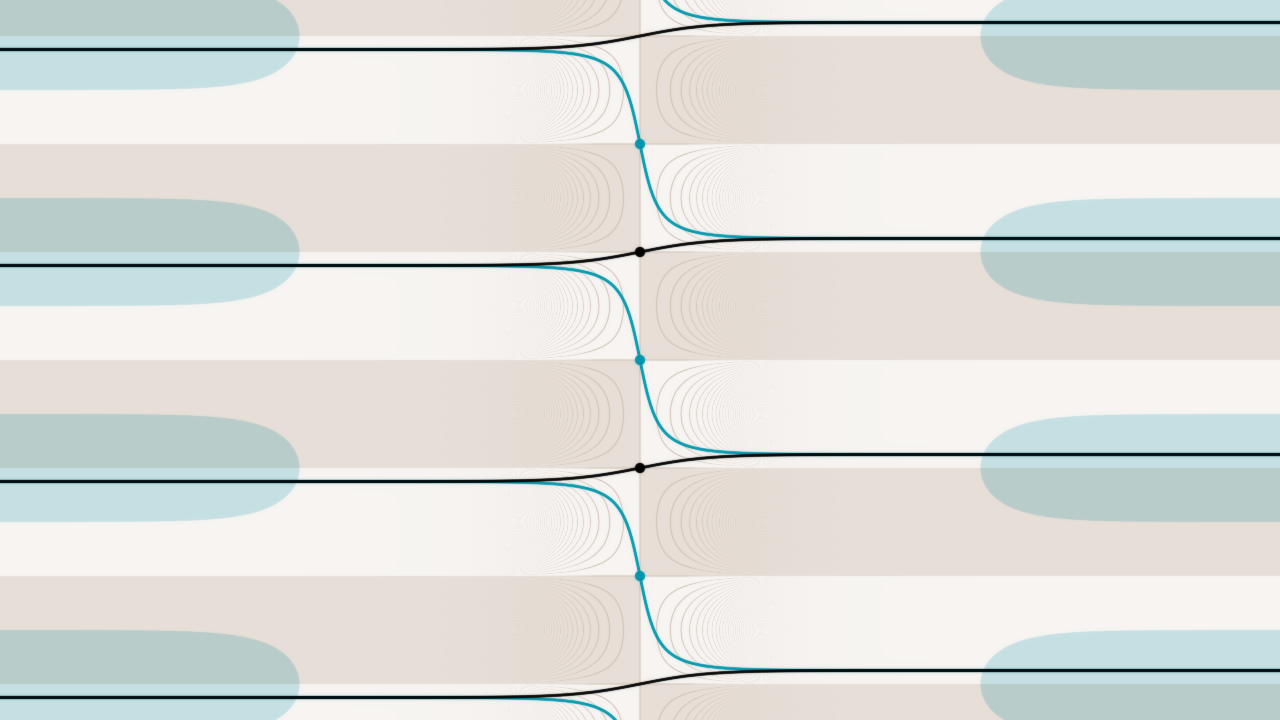
\includegraphics[width=10cm]{figures/bessel-unrolled.png}
\captionof{figure}{The paths $\mathcal{C}^{\pi/8}_j$ in the $t$ plane.}\label{fig:bessel_unrolled}
\end{center}

For any $\mu \in \C \smallsetminus \Z$, the classical modified Bessel function $K_\mu(z)$ can be expressed as the thimble integral
\begin{equation}\label{int:mod-bessel-gen}
 K_\mu(z) = \frac{1}{2 \sinh(\mu i\pi)} \int_{\mathcal{C}^\theta_1} \exp\left[z \cosh(t)\right]\,\sinh(\mu t)\,dt
\end{equation}
for $|\theta| < \tfrac{\pi}{2}$. This formula can be deduced, with a lot of finagling, from formulas 10.32(ii) and 10.27.4 of \cite{dlmf}\begin{todo}{[Cite Watson too?]}\end{todo}.
\begin{verify}
\par
From equation~6.22(3) of Watson's \textit{A treatise on the theory of Bessel functions} (1944), p. 181 (the reference in \cite{dlmf}):
\begin{align*}
2\pi i \, I_\mu(z) &= \int_{+\infty}^0 e^{z\cosh(-\pi i+a)-\mu(-i\pi +a)}\,da + \int_{0}^{+\infty} e^{z\cosh(\pi i+a)-\mu(i\pi +a)}\,da +\int_{-\pi}^{\pi} e^{z\cosh(ib)-\mu i b}\,db\\
& = -\int_{-\infty}^0 e^{z\cosh(-\pi i-a)+\mu(i \pi +a)}\,da + \int_{0}^{+\infty} e^{z\cosh(\pi i+a)-\mu(i \pi  +a)}\,da +\int_{0}^{\pi} e^{z\cosh(ib)}\cosh(i\mu b)\,db\\
& = -\int_{-\infty}^0 e^{z\cosh(\pi i+a)+\mu(i\pi +a)}\,da + \int_{0}^{+\infty} e^{z\cosh(\pi i+a)-\mu(i\pi +a)}\,da +\int_{0}^{\pi} e^{z\cosh(ib)}\cosh(i\mu b)\,db.
\end{align*}
Hence,
\begin{align*}
4 i \sin(\mu \pi) K_\mu(z) & = 2\pi i \big[ I_{-\mu}(z) - I_\mu(z) \big] \\
& = \int_{-\infty}^0 e^{z\cosh(\pi i+a)}\left[-e^{-\mu(i\pi +a)}+e^{\mu(i\pi +a)}\right]\,da + \int_{0}^{+\infty} e^{z\cosh(\pi i+a)}\left[e^{\mu(i\pi +a)}-e^{-\mu(i\pi +a)}\right]\,da \\
& = 2\int_{-\infty}^0 e^{z\cosh(\pi i+a)} \sinh\big(\mu(a+i\pi)\big)\,da + 2\int_{0}^{+\infty} e^{z\cosh(\pi i+a)} \sinh(\mu(i\pi+a)\big)\,da.
\end{align*}
This simplifies to the integral
\[ 2 \int_\gamma e^{z\cosh(t)} \sinh(\mu t)\,dt \]
along the contour $\gamma$ that runs rightward along $i\pi + \R$.
\par
\end{verify}
The integral converges when $z$ is in the right half-plane. Choosing a rational parameter $\mu = \tfrac{m}{n}$ gives formula~\eqref{integral:mod-bessel-lifted}, showing that $K^{(j)}_{m/n}(z)$ is the classical modified Bessel function $K_{m/n}(z)$ when $j$ is odd.

We can now apply the thimble projection formula, using the same reasoning as in Section~\ref{contour-argument-AL}. We first recast the integral into the $\zeta$ plane by setting $-\zeta = \cosh(t)$. This gives us the expression
\[ K^{(j)}_\mu(z) = -\frac{1}{2\sinh(\mu i\pi)} \int_{\mathcal{J}^\theta_{\zeta, \mp 1}} e^{-z\zeta} \left[ \frac{\sinh(\mu t_+)}{\sinh(t_+)} - \frac{\sinh(\mu t_-)}{\sinh(t_-)} \right] d\zeta, \]
where $t_-$ and $t_+$ are the lifts to the incoming and outgoing branches of $\mathcal{C}^\theta_j$. We then use identity~15.4.16 from \cite{dlmf} to write the integral explicitly in terms of $\zeta$:
\begin{align*}
\frac{\sinh(\mu t)}{\sinh(t)} & = \mu\;{}_2F_1\left(\frac{1}{2} - \frac{\mu}{2},\;\frac{1}{2} + \frac{\mu}{2};\;\frac{3}{2};\;-\sinh(t)^2\right) \\
& = \mu\;{}_2F_1\left(\frac{1}{2} - \frac{\mu}{2},\;\frac{1}{2} + \frac{\mu}{2};\;\frac{3}{2};\;1 - \zeta^2\right).
\end{align*}
Like before, we can deduce by analytic continuation that this identity holds throughout the $t$ plane.

Using formula~15.8.4 from \cite{dlmf}, followed by formulas 15.8.27 and 15.8.28 from the same source, we can repeat the arguments of Section~\ref{contour-argument-AL}, eventually rewriting the integrand as the variation of the function
\[ \frac{\sinh(\mu t)}{\sinh(t)} = \frac{3\mu}{2}\;{}_2F_1\left(1 - \mu,\;1 + \mu;\;\frac{3}{2};\frac{1}{2} - \frac{\zeta}{2}\right) + \frac{\mu}{2}\;{}_2F_1\left(1 - \mu,\;1 + \mu;\;\frac{3}{2};\;\frac{1}{2} + \frac{\zeta}{2}\right) \]
across the branch cut $\mathcal{J}^\theta_{\zeta, \mp 1}$. As before, the term that contributes to the jump is the one which is singular at the critical value where the branch cut starts. We use identity~15.2.3 from \cite{dlmf} to write the jump explicitly. For odd $j$, we get
\begin{equation}\label{eq: K_j_mu at 1}
  K^{(j)}_\mu(z) = -\frac{1}{2} \int_{\mathcal{J}^\theta_{\zeta, 1}} e^{-z\zeta} \left(-\frac{1}{2}+\frac{\zeta}{2}\right)^{-1/2} {}_2F_1\left(\frac{1}{2} - \mu,\;\frac{1}{2} + \mu;\;\frac{1}{2};\;\frac{1}{2} - \frac{\zeta}{2}\right) d\zeta,  
\end{equation}
and for even $j$, we get
\begin{equation}\label{eq: K_j_mu at -1}
 K^{(j)}_\mu(z) = \frac{3}{2} \int_{\mathcal{J}^\theta_{\zeta, -1}} e^{-z\zeta} \left(-\frac{1}{2}-\frac{\zeta}{2}\right)^{-1/2} {}_2F_1\left(\frac{1}{2} - \mu,\;\frac{1}{2} + \mu;\;\frac{1}{2};\;\frac{1}{2} + \frac{\zeta}{2}\right) d\zeta. 
\end{equation}

% \color{black}
% \par\textcolor{orange}{[Old text\ldots]}
% \color{RoyalBlue}
% \begin{align*}
%     K_\mu(z)& = -\frac{1}{2 \sinh(\mu\,i\pi)} \int_{\gamma_z} e^{-z \zeta}\,\frac{\sinh(\mu t)}{\sinh(t)}\,d\zeta  & \\
%     &=-\frac{\mu}{2 \sinh(\mu\,i\pi)} \int_{\gamma_z} e^{-z \zeta}\, {}_2F_1\left(\frac{1+\mu}{2},\frac{1-\mu}{2};\frac{3}{2};1-\zeta^2\right)\,d\zeta & \cite[15.4.16]{dlmf}
% \end{align*}
% where $\gamma_z$ is Hankel contour coming from $\infty$ to $1$ and then going back to $\infty$. Using formula \cite[15.8.4]{dlmf}, followed by \cite[15.8.27]{dlmf} and \cite[15.8.28]{dlmf} \textcolor{PaleVioletRed}{[Please clean up operators that are repeated across line breaks, like the $=$ below. I like the equation spacing in the ``Thimble projection reasoning for Airly-Lucas functions'' section; can we copy that here?]}
% \begin{multline*}
%      {}_2F_1\left(\frac{1+\mu}{2},\frac{1-\mu}{2};\frac{3}{2};1-\zeta^2\right) \textcolor{magenta}{=} \\
%      =\frac{3}{2}\, {}_2F_1\left(1-\mu,1+\mu,\frac{3}{2};\frac{1-\zeta}{2}\right)+\frac{1}{2}\, {}_2F_1\left(1-\mu,1+\mu,\frac{3}{2};\frac{1+\zeta}{2}\right)
% \end{multline*}
% hence 
% %
% \[K_\mu(z)=\frac{\mu\, i}{4 \sin(\mu\pi)} \int_{\gamma_z} e^{-z \zeta}\, {}_2F_1\left(1-\mu,1+\mu;\frac{3}{2};\frac{1+\zeta}{2}\right)\,d\zeta\]
% %
% Equation \cite[15.2.3]{dlmf} gives the analytic continuation of hypergeometric functions across the branch cut:

% \begin{align}
%     K_{\mu}(z)& \label{eqn:K-mu}=-\frac{1}{2}\int_1^\infty e^{-z\zeta} \, \left(\frac{\zeta-1}{2}\right)^{-1/2} \,\, {}_2F_1\left(\frac{1}{2}-\mu, \frac{1}{2}+\mu;\frac{1}{2};\frac{1-\zeta}{2}\right)  d\zeta\\
%     &  \notag=-\frac{i}{2}\laplace_{\zeta,1} v_{\mu,1} . 
% \end{align}
% \color{black}
\subsubsection{The modified Bessel function with parameter $0$}\label{sec:bessel-0}
When $\mu$ goes to $0$, formula~\eqref{int:mod-bessel-gen} becomes
\[ K_0^{(j)}(z) = \frac{1}{2\pi i} \int_{\mathcal{C}_j^\theta} \exp\left[z \cosh(t)\right]\,t\,dt. \]
Let us compute $K^{(1)}_{0}(z)$ using the contour $\mathcal{C}_1^0$, which runs rightward along the line $\Im(t) = \pi$. In the translated coordinate $w$ defined by $t = w + i\pi$, the integral becomes
\begin{align*}
K_0^{(1)}(z) & = \frac{1}{2\pi i} \int_{-\infty}^\infty \exp\left[z \cosh(w + i\pi)\right]\,(w + i\pi)\,dw \\
& = \frac{1}{2\pi i} \int_{-\infty}^\infty \exp\left[-z \cosh(w)\right]\,w\,dw + \frac{1}{2\pi i} \int_{-\infty}^\infty \exp\left[-z \cosh(w)\right]\,i\pi\,dw.
\end{align*}
The first integrand is odd with respect to $w = 0$, so it vanishes, leaving
\begin{align}
K_0^{(1)}(z) & = \frac{1}{2} \int_{-\infty}^\infty \exp\left[-z \cosh(w)\right]\,dw \notag \\
& = \int_0^\infty \exp\left[-z \cosh(w)\right]\,dw. \label{int:k0_cosh}
\end{align}
This is a special case of formula~10.32.9 from \cite{dlmf}. Rolling the $t$ plane up into a cylinder, parameterized by the coordinate $s = e^t$, we can express $K_0^{(1)}(z)$ as an exponential period:
\[ K_0^{(1)}(z) = \int_{\mathcal{J}^0_{s, 1}} \exp\left[-z\,\tfrac{1}{2}\left(s + \tfrac{1}{s}\right)\right]\,\frac{ds}{s}. \]

To confirm that the calculation above is consistent with Section~\ref{countable-cover}, recall formula~\eqref{eq: K_j_mu at 1}:
\[ K_0^{(1)}(z) = -\frac{1}{2} \int_{\mathcal{J}^\theta_{\zeta, 1}} e^{-z\zeta} \left(-\frac{1}{2}+\frac{\zeta}{2}\right)^{-1/2} {}_2F_1\left(\frac{1}{2},\;\frac{1}{2};\;\frac{1}{2};\;\frac{1}{2} - \frac{\zeta}{2}\right) d\zeta. \]
The hypergeometric function in the integrand can be expressed algebraically using identity~15.4.13 from \cite{dlmf}. This leads to an expression for the integrand that makes its $\zeta_{\pm 1}^{1/2}$ singularities even more apparent:
\begin{equation}\label{eqn:borel_bessel0}
K_0^{(1)}(z) = \int_{\mathcal{J}^\theta_{\zeta, 1}} e^{-z\zeta}\,\big(\zeta^2 - 1\big)^{-1/2}\;d\zeta.
\end{equation}
We could get the same result from formula~\eqref{int:k0_cosh} by trigonometric substitution. This is a special case of formula~10.32.8 from \cite{dlmf}.
%
\subsection{Generalized Airy}\label{sec:gen-airy}
%
In \cite{Reid} and the appendix of \cite{drazin-reid}, Drazin and Reid construct approximate solutions of the Orr--Sommerfield fluid equation using the generalized Airy functions
\begin{align*}
\mathrm{A}_k(y,p) & = \frac{1}{2\pi i}\int_{\mathscr{a}_k} \exp\big[yt-\tfrac{t^3}{3}\big]\,\frac{dt}{t^p} & & p \in \C\hphantom{{}_{\le 0}},\quad k \in \{1,2,3\} \\
\mathrm{B}_0(y,p) & = \frac{1}{2\pi i}\int_{\mathscr{b}_0} \exp\big[yt-\tfrac{t^3}{3}\big]\,\frac{dt}{t^p} & & p \in \Z \\
\mathrm{B}_k(y,p) & = \hphantom{\frac{1}{2\pi i}} \int_{\mathscr{b}_k} \exp\big[yt-\tfrac{t^3}{3}\big]\,\frac{dt}{t^p}, & & p \in \Z_{\le 0},\quad k \in \{1,2,3\}
\end{align*}
which are defined by integrals along the contours $\mathscr{a}_k, \mathscr{b}_0, \mathscr{b}_k$ shown in Figure~\ref{fig:path-generalized-Airy}~\cite{drazin-reid}\cite[Section 9.13(ii)]{dlmf}.
\begin{figure}[ht]
\center
\newcommand{\apathcolor}{ietcoast}
\newcommand{\bpathcolor}{black}
\begin{tikzpicture}
\renewcommand{\dotsize}{0.08}
\fill[pwbeige!10] circle(3.95);
\begin{scope}[\bpathcolor, very thick, -stealth]
  \draw (80:0.8) arc (80:400:0.8);
  \node at (60:0.8) {$\mathscr{b}_0$};
  \foreach \ang/\name in {0/1, 120/2, 240/3} {
    \draw[very thick,-stealth] (0, 0) -- ++(\ang:4) node[anchor=\ang-180] {$\mathscr{b}_\name$};
  };
  \fill (1.25, 0) circle (\dotsize) node[anchor=north west] {$\tfrac{1}{2}$};
  \draw[fill=white, thin] circle (\dotsize);
\end{scope}
\begin{scope}[\apathcolor, very thick, -stealth]
  \foreach \ang/\name in {0/1, 120/2, 240/3} {
    \draw[rotate=\ang] (-0.5, 0) +(-120:3.75) .. controls +(62:1) and +(0, -1.2) .. +(-0.75, 0) .. controls +(0, 1.2) and +(-62:1) .. +(120:3.75) node[midway, anchor=\ang+30] {$\mathscr{a}_\name$};
  };
  \fill (-1.25, 0) circle (\dotsize) node[anchor=north east] {$-\tfrac{1}{2}$};
\end{scope}
\end{tikzpicture}
\caption{The integration contours in the $t$ plane that define $\mathrm{A}_k,\mathrm{B}_0,\mathrm{B}_k$.}\label{fig:path-generalized-Airy}
\end{figure}
These functions satisfy the generalized Airy equation
\[ \left[\big(\tfrac{\partial}{\partial y}\big)^3 - y\,\tfrac{\partial}{\partial y} + (p-1)\right] \Phi = 0. \]
When $p = 0$, this equation reduces to
\[ \tfrac{\partial}{\partial y} \circ \left[\big(\tfrac{\partial}{\partial y}\big)^2 - y\right] \Phi = 0, \]
which is equivalent to an inhomogeneous version of the classical Airy equation.

As we did with the Airy--Lucas functions, we will use the substitution $t = 2uy^{1/2}$ to rewrite the generalized Airy function $\mathrm{A}_1(y,p)$ in terms of a thimble integral. We get
\[ \mathrm{A}_1(y,p) = (12 z)^{(1-p)/3}\,I_+\big(\tfrac{2}{3}y^{3/2},p\big) \]
with
\[ I_+(z,p) = \frac{1}{2\pi i} \int_{\mathcal{C}^\theta_1} \exp\left[-z\left(4u^3 - 3u\right)\right]\,\frac{du}{u^p}. \]
To find the right contour $\mathcal{C}_1^\theta$, we first note that the mapping $\zeta = 4u^3 - 3u$ is familiar, up to a sign, from Section~\ref{sec:airy}. In particular, we already know its critical points $u = \pm\tfrac{1}{2}$ and the corresponding critical values $\zeta = \pm 1$. To get the desired integral, $\mathcal{C}_1^\theta$ should be the thimble through $u = -\tfrac{1}{2}$ over the ray $\mathcal{J}^\theta_1$. However, this thimble does not live on the complex plane, like it did for the classical Airy function. When $p$ is a positive integer, the volume form $du/u^p$ has a pole at $u = 0$, so we put $\mathcal{C}_1^\theta$ as a contour on $\C^\times$. More generally, for any complex value of $p$, we can put $\mathcal{C}_1^\theta$ on the universal cover $\widetilde{\C^\times}$.
\begin{verify}
\begin{align*}
I_{+}(z,p)&=\frac{1}{2\pi i}\int_{\mathcal{C}_{+}}e^{-z(4u^3-3u)}\, \frac{du}{u^p} &\\
&=\frac{1}{2\pi i}(12 z)^{(p-1)/3}\int_{z^{1/3}\mathcal{C}_{+}}e^{-z(\tfrac{4}{12}\tfrac{t^3}{z}-3 (12 z)^{-1/3}t)}\frac{dt}{t^p} & u=(12 z)^{-\tfrac{1}{3}}t\\
&=\frac{1}{2\pi i}(12 z)^{(p-1)/3}\int_{z^{1/3}\mathcal{C}_{+}}e^{-\left(\frac{t^3}{3}-(\tfrac{3}{2} z)^{2/3}t\right)}\frac{dt}{t^p} & \\
&=(12 z)^{(p-1)/3}\mathrm{A}_1((\tfrac{3}{2}z)^{2/3},p)
\end{align*}  
\end{verify}
%
We will now show, in the case $p = 1$, that equation~\eqref{eqn:I} has a frame of Borel regular solutions---as long as the constant solution $\mathrm{B}_0(z, 1)$ counts as Borel regular. For $\mathrm{A}_1(y, p)$ to satisfy the generalized Airy equation, $I_+(z,1)$ must satisfy the equation
\begin{equation}\label{eqn:I}
\left[\big[\big(\tfrac{\partial}{\partial z}\big)^2 - 1\big] + z^{-1} \left(\tfrac{\partial}{\partial z}\right)^2 - \tfrac{1}{9} z^{-2} \right] \tfrac{\partial}{\partial z} \Phi = 0.
\end{equation}
Equivalently, $\tfrac{\partial}{\partial z} I_+(z, 1)$ satisfies the modified Bessel equation \eqref{eqn:reg-mod-bessel-AL} with parameter $1/3$. We can now follow the reasoning of Section~\ref{big-idea}, viewing that frequency domain differential equation~\eqref{eqn:I} as the image under $\laplace_{\zeta, \alpha}$ of the position domain integral equation
\begin{equation}\label{int-eq:position-I}
\left[ \big[ \zeta^2 - 1 \big] - \fracderiv{-1}{\zeta}{\alpha} \circ \zeta - \big(\tfrac{1}{3}\big)^2 \fracderiv{-2}{\zeta}{\alpha} \right] (-\zeta)\,v^{(1)} = 0.
\end{equation}
In Sections \ref{pos-root-AL} and \ref{neg-root-AL}, we found solutions $v_{\pm 1}$ of the closely related equation~\eqref{int-eq:spatial-mod-bessel-AL}, which we can turn into solutions $v^{(1)}_{\pm 1} = \zeta^{-1} v_{\pm 1}$ of equation~\eqref{int-eq:position-I}.

At the critical values $\zeta = \pm 1$, we can build solutions $v^{(1)}_{\pm 1}$ of this equation from the solutions $v_{\pm 1}$ of equation~\eqref{int-eq:spatial-mod-bessel-AL} that we found in Sections \ref{pos-root-AL} and \ref{neg-root-AL}. Explicitly, in terms of the coordinates defined by $\zeta = 1 + \zeta_1$ and $\zeta = -1 + \zeta_{-1}$, these solutions are
\begin{alignat*}{3}
v^{(1)}_1 &=\;& -i\sqrt{2}\,(1 + \zeta_1)^{-1} &\,\zeta_1^{-1/2} &\;{}_2F_1\big(\tfrac{1}{6},\tfrac{5}{6};\tfrac{1}{2};-\tfrac{1}{2}\zeta_{1}\big) \\
v^{(1)}_{-1} &=\;& \sqrt{2}\,(-1 + \zeta_{-1})^{-1} &\,\zeta_{-1}^{-1/2} &\;{}_2F_1\big(\tfrac{1}{6},\tfrac{5}{6};\tfrac{1}{2};\tfrac{1}{2}\zeta_{-1}\big).
\end{alignat*}
Their Laplace transforms $V^{(1)}_1 = \laplace_{\zeta, 1} v^{(1)}_1$ and $V^{(1)}_{-1} = \laplace_{\zeta, -1} v^{(1)}_{-1}$ satisfy equation~\eqref{eqn:I}.
\begin{verify}
From the result about the Bessel equation, we know there exists two analytic functions $v_1$ and $v_{-1}$ such that $\varphi_1$ and $\varphi_2$ defined by $\partial_z\varphi_1=\laplace_{\zeta,1}v_1$ and $\partial_z\varphi_2=\laplace_{\zeta,-1}v_{-1}$, give a frame of analytic solutions of \eqref{eqn:I}. Then we argue as follows:
\begin{align*}
    \partial_z\varphi_1&=\laplace_{\zeta,1}v_1\\
    \varphi_1-\varphi_1(a)&=\int_a^z\int_1^{\infty}e^{-y\zeta} v_1 d\zeta \, dy\\
    &=\int_1^{\infty}d\zeta\,  v_1 \, \int_a^ze^{-y\zeta}  \, dy\\
    &=\int_1^{\infty}d\zeta\,  v_1 \, \Big[\frac{e^{-\zeta a}}{\zeta}-\frac{e^{-z\zeta}}{\zeta}\Big]\\
    &=\laplace_{\zeta,1} \tfrac{v_1}{\zeta}-\Big[\laplace_{\zeta,1}\tfrac{v_1}{\zeta}\Big](a)
\end{align*}
\end{verify}
Notice that $v^{(1)}_1$ belongs to $\singexpalg{-1/2}(\Omega_1)$, has a simple pole at $\zeta_1 = -1$, and has a logarithmic singularity at $\zeta_1 = -2$. Similarly, $v^{(1)}_{-1}$ belongs to $\singexpalg{1/2}(\Omega_{-1})$, has a simple pole at $\zeta_{-1} = 1$, and has a logarithmic singularity at $\zeta_{-1} = 2$.

With an argument analogous to the one in Section~\ref{bessel-regularity-AL}, one should be able to show that $V^{(1)}_1$ and $V^{(1)}_{-1}$ are Borel regular. Since equation~\eqref{eqn:I} is third-order, we need one more Borel regular solution to make a frame. We choose the constant solution $1$, which can be seen as the Laplace transform of the formal convolution unit $\delta$ introduced in Section~\ref{sec:borel-laplace-homom}. Interestingly, $1$ is actually the generalized Airy function $\mathrm{B}_0(z,1)$.
%
\begin{todo}
\subsubsection{Thimble projection formula}
In Theorem~\ref{thm:maxim-proof}, we proved a $3/2$-derivative formula to compute the Borel transform of the asymptotics of a thimble integral.
\color{black}
\end{todo}
\subsection{Third-degree thimble integrals}\label{sec:deg3}
In this section, we consider the thimble integral
\[ I(z) = \int_{\mathcal{C}} e^{-zg}\,du \]
defined by a general third-degree polynomial map $g \maps \C \to \C$. By definition, the Lefschetz thimble $\mathcal{C}$ is a connected component of the preimage of a critical value of $g$. After taking various symmetries into account, we will find that there are essentially only two cases, distinguished by whether $g$ has two distinct critical points or a single degenerate one.
\subsubsection{Symmetries of the integral}\label{sec:int-symm}
First, we step back and consider the completely general thimble integral
\[ J(z) = \int_{\mathcal{C}} e^{-zf}\,\nu \]
defined by an arbitrary holomorphic map $f \maps X \to \C$ and an arbitrary $1$-form $\nu$ on $X$. The affine group of $\C$ acts on $f$ by post-composition, and this action affects $J$ in a simple way. The affine group is generated by two kinds of transformations, which we consider separately.
%%The affine group of $\C$ acts on $f$ by post-composition, and $\C^\times$ acts on $\nu$ by multiplication. These actions both affect $J$ in simple ways. The affine group is generated by two kinds of transformations, which we consider separately.
\begin{itemize}
\item[] \textbf{Translations}

For any $c \in \C$, the translation action $f \mapsto f + c$ on maps corresponds to the action
\[ J(z) \mapsto e^{-cz} J(z) \]
on integrals. This is because
\begin{align*}
\int_\mathcal{C} e^{-z(f + c)}\,\nu & = e^{-cz} \int_\mathcal{C} e^{-zf}\,\nu \\
& = e^{-cz} J(z).
\end{align*}
\item[] \textbf{Scaling-rotations}

For any $r \in \C^\times$, the scaling-rotation action $f \mapsto rf$ corresponds to the action
\[ J(z) \mapsto J(rz) \]
on integrals. This is because
\begin{align*}
\int_\mathcal{C} e^{-z(rf)}\,\nu & = \int_\mathcal{C} e^{-(rz)f}\,\nu \\
& = J(rz).
\end{align*}
%%\item[] \textbf{Multiplications}
%%
%%For any $s \in \C^\times$, the multiplication action $\nu \mapsto s\nu$ corresponds to the action
%%\[ J(z) \mapsto s J(z) \]
%%on integrals.
\end{itemize}
Next, we specialize to the case where $X$ is the complex plane and $\nu = du$, where $u$ is the standard coordinate. The affine group of $\C$ now acts on $f$ by pre-composition as well. To make sure that $\mathcal{C}$ remains a Lefschetz thimble, we act on it simultaneously by the inverse of whatever we precompose with $f$.
\begin{itemize}
\item[] \textbf{Translations}

For any $c \in \C$, pulling $f$ back along the translation $\mathsf{T}_c^* u = u - c$ has no effect on the integral. This is because $du$ is translation-invariant.

\item[] \textbf{Scaling-rotations}

For any $s \in \C^\times$, the scaling-rotation action $\mathsf{M}_s^* u = s^{-1} u$ corresponds to the action
\[ J(z) \mapsto s J(z) \]
on integrals. This is because
\begin{align*}
\int_{\mathsf{M}_{1/s} \mathcal{C}} e^{-z \mathsf{M}_s^* f}\,du & = \int_\mathcal{C} e^{-zf}\,\mathsf{M}_{1/s}^* du \\
& = \int_\mathcal{C} e^{-zf}\,s\,du \\
& = s J(z).
\end{align*}
%%\item[] \textbf{Multiplications}
%%
%%For any $s \in \C^\times$, the multiplication action $\nu \mapsto s\nu$ corresponds to the action
%%\[ J(z) \mapsto s J(z) \]
%%on integrals.
\end{itemize}
\subsubsection{Reduction of the integral}
We now return to our original thimble integral $I(z)$, defined by the third-degree polynomial map
\[ g = a_3 u^3 + a_2 u^2 + a_1 u + a_0, \]
and use the group actions from Section~\ref{sec:int-symm} to reduce it to its two essential cases. We first put $g$ in depressed form by scaling the leading coefficient to $1$ and translating the mean of the critical points to $0$.\footnote{The coefficients of the depressed form are related to the original coefficients as follows:
\begin{align*}
p & = \frac{a_1}{a_3} - \frac{1}{3} \left(\frac{a_2}{a_3}\right)^2 \\
q & = \frac{a_0}{a_3} - \frac{1}{3} \left(\frac{a_1}{a_3}\right)\left(\frac{a_2}{a_3}\right) + \frac{2}{27} \left(\frac{a_2}{a_3}\right)^3.
\end{align*}} We then also translate the mean of the critical values to $0$.
\begin{center}
\begin{tabular}{c|c|c}
\textbf{Symmetry} & \textbf{Resulting polynomial} & \textbf{Resulting integral} \\[2mm]
$\displaystyle f \mapsto \frac{f}{a_3}$ & $\displaystyle u^3 + \frac{a_2}{a_3} u^2 + \frac{a_1}{a_3} u + \frac{a_0}{a_3}$ & $\displaystyle \hphantom{e^{qz}} I\left(\frac{z}{a_3}\right)$ \\[5mm]
$\displaystyle \mathsf{T}_{(1/3)\,a_2/a_3}^*$ & $\displaystyle u^3 + pu + q$ & $\displaystyle \hphantom{e^{qz}} I\left(\frac{z}{a_3}\right)$ \\[5mm]
$\displaystyle f \mapsto f - q$ & $\displaystyle u^3 + pu$ & $\displaystyle e^{qz}\,I\left(\frac{z}{a_3}\right)$ \\[5mm]
\end{tabular}
\end{center}
Our next move depends on how many critical points $g$ has.
\begin{itemize}
\item[] \textbf{Two distinct critical points}

When $p$ is non-zero, $g$ has two distinct critical points. We can use our symmetries turn it into any other third-degree polynomial with distinct critical points. To illustrate, we turn $g$ into the Chebyshev polynomial $T_3$ by scaling and rotating its critical points to $\pm\tfrac{1}{2}$ and its critical values to $\pm 1$. Setting
\[ r \defeq \frac{i}{2} \left(\frac{3}{p}\right)^{3/2}, \]
we get
\begin{center}
\begin{tabular}{c|c|c}
\textbf{Symmetry} & \textbf{Resulting polynomial} & \textbf{Resulting integral} \\[2mm]
$\displaystyle \mathsf{M}_{rp/3}^*$ & $\displaystyle r^{-1} \left(-4u^3 + 3u\right)$ & $\displaystyle \frac{rp}{3}\,e^{qz}\,I\left(\frac{z}{a_3}\right)$ \\[5mm]
$\displaystyle f \mapsto rf$ & $\displaystyle -4u^3 + 3u$ & $\displaystyle \frac{rp}{3}\,e^{qrz}\,I\left(\frac{rz}{a_3}\right)$ \\[5mm]
\end{tabular}
\end{center}

We can now relate the general third-degree thimble integral $I$ to the modified Bessel function $K_{1/3}$, defined in equation~\eqref{integral:mod-bessel-rational-AL}:
\begin{equation}
K_{1/3}(z) = \frac{irp}{\sqrt{3}}\,e^{qrz}\,I\left(\frac{rz}{a_3}\right)
\end{equation}
\begin{verify}
\begin{equation}
K_{1/3}(z) = -\frac{3}{2}\,p^{-1/2} e^{-zq \frac{1}{2i} \left(\frac{3}{p}\right)^{3/2}}\,I\left(-\frac{1}{2i} \left(\frac{3}{p}\right)^{3/2} \frac{z}{a_3}\right).
\end{equation}
\end{verify}
From this identity, you can deduce that $I(z)$ satisfies a second-order differential equation, analogous to the modified Bessel equation~\eqref{eqn:mod-bessel}.
\begin{todo}\par
From this identity, we can see that $I(z)$ satisfies a transformed version of the modified Bessel equation:
\[ \left[ \big[\big(\tfrac{\partial}{\partial z}\big)^2 + 2a_3 q\,\tfrac{\partial}{\partial z} + a_3^2 (q^2 - r^{-2})\big] + z^{-1} \big(a_3 q + \tfrac{\partial}{\partial z}\big) - \tfrac{1}{9} z^{-2} \right] \Phi = 0 \]
\begin{verify}
With
\begin{align*}
w & = \frac{r}{a_3}\,z &
\frac{\partial}{\partial w} & = \frac{a_3}{r} \frac{\partial}{\partial z}
\end{align*}
we have
\[ K_{1/3}(z) = \frac{irp}{\sqrt{3}}\,e^{a_3 qw}\,I(w) \]

Let us rewrite for simpicilty $K_{1/3}(z)=\alpha e^{\beta z} I(\gamma z)$, then using that $K_{1/3}$ is a solution of the modified Bessel equation~\eqref{eqn:mod-bessel} we get
\begin{align*}
0 &= I''(\gamma z)+\frac{\beta^2-1}{\gamma^2}I(\gamma z)+\frac{2\beta}{\gamma}I'(\gamma z)+\frac{1}{z}\left(\frac{\beta}{\gamma^2}I(\gamma z)+\frac{I'(\gamma z)}{\gamma}\right)-\frac{1}{9\gamma^2}\frac{1}{z^2} I(\gamma z) \\
0 &= I''(t)+\frac{\beta^2-1}{\gamma^2}I(t)+\frac{2\beta}{\gamma}I'(t)+\frac{1}{t}\left(\frac{\beta}{\gamma}I(t)+I'(t)\right)-\frac{1}{9t^2} I(t)\\
0 &= I''(t)+\frac{\beta^2}{\gamma^2}I(t)-\frac{1}{\gamma^2}I(t)+\frac{2\beta}{\gamma}I'(t)+\frac{1}{t}\frac{\beta}{\gamma}I(t)+\frac{1}{t}I'(t)-\frac{1}{9t^2} I(t)\\
0 &= I''(t)+a_3^2q^2 I(t)-\frac{a_3^2}{r^2}I(t)+2a_3 qI'(t)+\frac{a_3 q}{t}I(t)+\frac{1}{t}I'(t)-\frac{1}{9t^2} I(t)
\end{align*}

Here's a double-check. Since $K_{1/3}(z)$ satisfies the modified Bessel equation~\eqref{eqn:mod-bessel},
\begin{align*}
\left[z^2 \big(\tfrac{\partial}{\partial z}\big)^2 + z \tfrac{\partial}{\partial z} - \big[\big(\tfrac{1}{3}\big)^2 + z^2\big]\right] K_{1/3}(z) & = 0 \\
\left[z^2 \big(\tfrac{\partial}{\partial z}\big)^2 + z \tfrac{\partial}{\partial z} - \big[\big(\tfrac{1}{3}\big)^2 + z^2\big]\right] \frac{irp}{\sqrt{3}}\,e^{a_3 qw}\,I(w) & = 0 \\
\left[\big(\tfrac{a_3}{r} w\big)^2 \big(\tfrac{r}{a_3} \tfrac{\partial}{\partial w}\big)^2 + \big(\tfrac{a_3}{r} w\big) \tfrac{r}{a_3} \tfrac{\partial}{\partial w} - \big[\big(\tfrac{1}{3}\big)^2 + \big(\tfrac{a_3}{r} w\big)^2\big]\right] e^{a_3 qw}\,I(w) & = 0 \\
\left[w^2\big(\tfrac{\partial}{\partial w}\big)^2 + w \tfrac{\partial}{\partial w} - \big[\big(\tfrac{1}{3}\big)^2 + \big(\tfrac{a_3}{r}\big)^2 w^2\big]\right] e^{a_3 qw}\,I(w) & = 0 \\
e^{a_3 qw} \left[w^2 \big(\tfrac{\partial}{\partial w} + a_3 q\big)^2 + w \big(\tfrac{\partial}{\partial w} + a_3 q\big) - \big[\big(\tfrac{1}{3}\big)^2 + \big(\tfrac{a_3}{r}\big)^2 w^2\big]\right] I(w) & = 0 \\
\left[w^2 \big[\big(\tfrac{\partial}{\partial w}\big)^2 + 2a_3 q \tfrac{\partial}{\partial w} + (a_3 q)^2\big] + w \big(\tfrac{\partial}{\partial w} + a_3 q\big) - \big[\big(\tfrac{1}{3}\big)^2 + \big(\tfrac{a_3}{r}\big)^2 w^2\big]\right] I(w) & = 0
\end{align*}
\end{verify}
\begin{verify}
Taking $p$ and $q$ to $0$ in
\[ \left[ \big[\big(\tfrac{\partial}{\partial z}\big)^2 + 2a_3 q\,\tfrac{\partial}{\partial z} + a_3^2 (q^2 - r^{-2})\big] + z^{-1} \big(a_3 q + \tfrac{\partial}{\partial z}\big) - \tfrac{1}{9} z^{-2} \right] \Phi = 0, \]
we get
\[ \left[ \big[\big(\tfrac{\partial}{\partial z}\big)^2 + z^{-1} \tfrac{\partial}{\partial z} - \tfrac{1}{9} z^{-2} \right] \Phi = 0\]
\end{verify}
\end{todo}
\item[] \textbf{One degenerate critical point}
When $p$ is zero, $g$ has a single degenerate critical point. Like we did in Appendix~\ref{airy-appendix} for the non-degenerate case, we will first study $I(z)$ by viewing it as a solution of an ODE, and we will then confirm our results using the thimble projection formula.

By differentiating under the integral, we can see that $I(z)$ satisfies the equation
\begin{equation}\label{eqn:degree-3-poly-1root}
\left[\frac{\partial}{\partial z} + \frac{1}{3z} +q \right] \Phi = 0.
\end{equation}
A function $\laplace_{\zeta,\alpha}^{\theta} v$ satisfies this equation if and only if $v$ satisfies the integral equation
\[ \left[ -\zeta + \tfrac{1}{3} \partial^{-1}_{\zeta, \alpha} +q  \right] v = 0. \]
When $\alpha = q$, this equation has the solution
\[ v_q = \zeta_q^{-2/3}, \]
whose Laplace transform
\[ V_q = e^{-zq} \Gamma\big(\tfrac{1}{3})\,z^{-1/3} \]
must be proportional to $I(z)$.

We can confirm this result, and find the correct normalization, using the thimble projection formula:
\begin{align*}
\int_{\mathcal{C}} e^{-z(u^3+q)}\,du & = (1 - e^{i\pi/3}) \int_{\mathcal{J}_{\zeta_q, 0}^\theta} e^{-z\zeta}\,\tfrac{1}{3}\zeta_q^{-2/3}\,d\zeta_q \\
& = e^{-zq}\tfrac{1}{i\sqrt{3}}\,e^{i\pi/3}\,\Gamma\big(\tfrac{1}{3})\,z^{-1/3}.
\end{align*}
The factor of $e^{i\pi/3} - 1$ comes from the monodromy of $\zeta_q^{-2/3}$ around $\zeta_q = 0$. 
\begin{brainstorm}
\item namely $v=(\zeta-q)^{-2/3}=\zeta_q^{-2/3}={}_2F_1\left(a,\frac{2}{3};a;1-\zeta_q\right)$, where $\zeta_q=\zeta-q$ and $a\in\C$ is a free parameter.
\end{brainstorm}
\end{itemize}
\subsubsection{Coalescence of critical values}
We can recover the degenerate case by taking the limit of the non-degenerate case as $p$ goes to zero. Rearranging the relationship above between $I(z)$ and the modified Bessel function $K_{1/3}(z)$, we get the formula
\[ I(z) = \frac{\sqrt{3}}{irp} e^{-qa_3z} K_{1/3}\left(\frac{a_3 z}{r}\right) \]
Setting $q=0$, and using the Taylor expansion of $K_{1/3}(z)$ around $z = 0$, given by equations 10.25.2 and 10.27.4 of \cite{dlmf}, we can see that $I(z)$ converges pointwise to $\tfrac{1}{i\sqrt{3}}\,e^{i\pi/3}\,\Gamma\big(\tfrac{1}{3}\big)\,z^{-1/3}$ as $p$ goes to zero with $a_3$ held constant.
\begin{verify}
\begin{align*}
I(z) & = \frac{\sqrt{3}}{irp} e^{-qrz} K_{1/3}\left(\frac{a_3 z}{r}\right) \\
& = \frac{\sqrt{3}}{irp} e^{-qrz} \frac{\pi}{2 \sin(\pi/3)} \left[ I_{-1/3}\left(\frac{a_3 z}{r}\right) - I_{1/3}\left(\frac{a_3 z}{r} \right)\right].
\end{align*}
We take the lowest-order term, which is the leading term of $I_{-1/3}(a_3 z / r)$:
\begin{align*}
I(z) & \approx \frac{\sqrt{3}}{irp} \frac{\pi}{2 \sin(\pi/3)} \left(\frac{a_3 z}{2r}\right)^{-1/3} \frac{1}{\Gamma\big(-\tfrac{1}{3} + 1\big)} \\
& = \frac{\sqrt{3}}{irp}\;\frac{1}{2}\;\Gamma\big(\tfrac{1}{3}\big)\,\Gamma\big(\tfrac{2}{3}\big) \left(\frac{a_3 z}{2r}\right)^{-1/3} \frac{1}{\Gamma\big(\tfrac{2}{3}\big)} \\
& = \frac{\sqrt{3}}{irp}\;\frac{1}{2}\;\Gamma\big(\tfrac{1}{3}\big)\,\Gamma\big(\tfrac{2}{3}\big) \left(\frac{a_3 z}{2r}\right)^{-1/3} \frac{1}{\Gamma\big(\tfrac{2}{3}\big)} \\
& = \frac{\sqrt{3}}{i a_3^{1/3} (2r)^{2/3} p} \Gamma\big(\tfrac{1}{3}\big)\;z^{-1/3} \\
& = \frac{\sqrt{3}}{i a_3^{1/3} (2r)^{2/3} p} \Gamma\big(\tfrac{1}{3}\big)\;z^{-1/3}.
\end{align*}
Observing that $(2r)^{2/3} = e^{i(2/3)\pi }\,3/p$, we get
\begin{align*}
I(z) & \approx \frac{\sqrt{3}}{i a_3^{1/3}\,3e^{i(2/3)\pi}} \Gamma\big(\tfrac{1}{3}\big)\;z^{-1/3} \\
& = \frac{1}{i\sqrt{3}} a_3^{-1/3} e^{i\pi/3}\,\Gamma\big(\tfrac{1}{3}\big)\;z^{-1/3}
\end{align*}
\end{verify}
%
\subsection{The triangular cantilever}\label{sec:catilever}
%
\subsubsection{Setting}
A {\em triangular cantilever} is a flexible strip with constant thickness and linearly tapered width, clamped at the broad end so it sticks out horizontally like a diving board.
\begin{center}
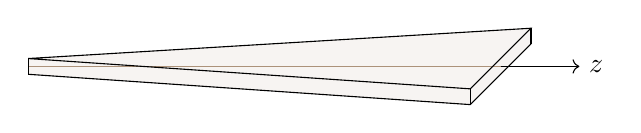
\begin{tikzpicture}
\newcommand{\clen}{6}
\newcommand{\ctaper}{1}
\newcommand{\cthic}{0.1}
\fill[pwbeige!10] (0, \cthic, 0) -- ++(6, 0, -\ctaper) -- ++(0, -2*\cthic, 0) -- ++(0, 0, 2*\ctaper) -- (0, -\cthic, 0);
\draw (0, -\cthic, 0) -- ++(\clen, 0, \ctaper) -- ++(0, 0, -2*\ctaper);
\draw[pwbeige] (0, 0, 0) -- ++(\clen, 0, 0);
\draw[->] (\clen, 0, 0) -- ++(1, 0, 0) node[anchor=west] {$z$};
\draw (0, \cthic, 0) -- ++(\clen, 0, \ctaper) -- ++(0, 0, -2*\ctaper) -- cycle;
\foreach \x / \y in {0 / 0, 6 / 1, 6 / -1} {
  \draw (\x, 0.1, \y) -- (\x, -0.1, \y);
}
\end{tikzpicture}
\end{center}
If you strike the strip from above, it vibrates up and down. Let us suppose the vibrations are small, and uniform across the width of the strip, so we can describe them using the Euler--Bernoulli beam model~\cite[\S 12.4]{genta2009vibration}. The vibration modes of frequency $\omega$ are described by the vertical displacement profiles $\Phi$ that satisfy the equation
\begin{equation}\label{eqn:triangular_cantilever}
    \left[\big[\big(\tfrac{\partial}{\partial z}\big)^4 - \omega^2\big] + \tfrac{2}{z}\big(\tfrac{\partial}{\partial z}\big)^3\right] \Phi = 0,
\end{equation}
where $z$ is the distance from the tip along the strip's axis.\footnote{To keep the equation simple, we've adjusted the units of time so that the strip's elasticity, density, and taper are absorbed into the frequency parameter.}

\begin{verify}
The vertical displacement of a vibrating beam is annihilated by the operator
\[ \big(\tfrac{\partial}{\partial z}\big)^2 \circ EI_\text{roll} \circ \big(\tfrac{\partial}{\partial z}\big)^2 + m \big(\tfrac{\partial}{\partial t}\big)^2, \]
as described in equation~12.58 of \cite{genta2009vibration}. Here, $m$ is the mass per unit length, $E$ is the elastic modulus, and $I_\text{roll}$ is the second moment of area about the axis the beam ``rolls'' around as it vibrates. We can write the displacement as $\cos(\omega t)$ times a time-independent envelope, which is annihilated by the operator
\[ \mathcal{P} = \big(\tfrac{\partial}{\partial z}\big)^2 \circ EI_\text{roll} \circ \big(\tfrac{\partial}{\partial z}\big)^2 - m\omega^2. \]
We are assuming the cantilever has a rectangular cross-section with half-width $s$ and half-thickness $t$, so its second moment of area about the side-to-side axis is $\tfrac{4}{3}st^3$, mass per unit length isproportional to $st$, giving
\[ \mathcal{P} = \big(\tfrac{\partial}{\partial z}\big)^2 \circ \tfrac{4}{3}Et^3 s \circ \big(\tfrac{\partial}{\partial z}\big)^2 - t\omega^2 s. \]
For the triangular cantilever, $t$ is constant, and $s = \sigma z$ for some constant $\sigma$. Letting $c_1 = \tfrac{4}{3}\sigma Et^3$ and $c_2 = t\sigma\omega^2$, we have
\begin{align*}
\mathcal{P} & = \big(\tfrac{\partial}{\partial z}\big)^2 \circ c_1 z \circ \big(\tfrac{\partial}{\partial z}\big)^2 - c_2 z \\
& = c_1 \tfrac{\partial}{\partial z} \circ \big[ 1 + z \tfrac{\partial}{\partial z} \big] \circ \big(\tfrac{\partial}{\partial z}\big)^2 - c_2 z \\
& = c_1 \circ \big[ \tfrac{\partial}{\partial z} + \tfrac{\partial}{\partial z} + z \big(\tfrac{\partial}{\partial z}\big)^2 \big] \circ \big(\tfrac{\partial}{\partial z}\big)^2 - c_2 z \\
& = c_1 2\big(\tfrac{\partial}{\partial z}\big)^3 + c_1 z \big(\tfrac{\partial}{\partial z}\big)^4 - c_2 z \\
\tfrac{1}{c_1 z} \mathcal{P} & = \tfrac{2}{z} \big(\tfrac{\partial}{\partial z}\big)^3 + \big(\tfrac{\partial}{\partial z}\big)^4 - \tfrac{c_2}{c_1}.
\end{align*}
Now, set $\mu = \tfrac{c_2}{c_1} = \tfrac{3}{4} \tfrac{1}{E} \big(\tfrac{\omega}{t}\big)^2$. This example works because the linear density of the beam and the second moment of area about the side-to-side axis are proportional, so they both end up in the $P(\partial/\partial z)$ term.\par
\end{verify}
\color{black}
\subsubsection{Solving the differential equation}
We seek functions $v$ and points $\zeta = \alpha$ for which the Laplace transform $\laplace_{\zeta, \alpha} v$ satisfies the differential equation~\eqref{eqn:triangular_cantilever}. From Proposition~\ref{prop:L-int-op} we deduce that $\laplace_{\zeta, \alpha} v$ satisfies equation~\eqref{eqn:triangular_cantilever} if and only if $v$ satisfies the integral equation
\begin{equation}\label{eqn:position_cantilever}
\left[ \big[ \zeta^4 - \omega^2 \big] - 2\fracderiv{-1}{\zeta}{\alpha} \circ \zeta^3 \right] v = 0.
\end{equation}
Observing that
\[ \tfrac{\partial}{\partial \zeta} \sqrt{\zeta^4 - \omega^2} = \frac{2\zeta^3}{\sqrt{\zeta^4 - \omega^2}}, \]
we learn that
\begin{equation}
v_\text{uni} = \frac{1}{\sqrt{\zeta^4 - \omega^2}}
\end{equation}
satisfies equation~\eqref{eqn:position_cantilever} whenever $\alpha^4 - \omega^2 = 0$. Thus, a single ``universal solution'' in the position domain leads to four linearly independent solutions $V_\alpha = \laplace_{\zeta, \alpha} v_\text{uni}$ of equation~\eqref{eqn:triangular_cantilever}, indexed by the fourth roots of $\omega^2$.
\subsubsection{Expressing the solutions as thimble integrals}
We can now use the thimble projection formula, as written in equation~\eqref{thimble-difference}, to express the solutions found above as thimble integrals. In terms of the Jacobi elliptic function $\operatorname{sd}$, we have
\begin{equation}\label{eq:cantilever-thimble}
V_\alpha = \int_{\mathcal{C}_a^\theta} \exp\left[ -z\,2i\omega \operatorname{sd}\big(u, \tfrac{1}{\sqrt{2}}\big) \right]\;du,  \end{equation}
where $a$ is a preimage of $\zeta = \alpha$ under the map $\zeta = 2i\omega \operatorname{sd}\big(u, \tfrac{1}{\sqrt{2}}\big)$. \begin{todo}[Show thimble picture.]\end{todo} Since exponent is doubly periodic, with period lattice $L = \tfrac{1}{\sqrt{2}}\Z + i\Z$, we can take the thimble to be a real submanifold of the torus $\C / L$.

To confirm equation~\eqref{eq:cantilever-thimble}, use Jacobi's transformations to rewrite the relationship between $\zeta$ and $u$ in terms of $\operatorname{sn}$.
\[ \zeta = \omega^{1/2} \operatorname{sn}\big(2i \omega^{1/2} u, i\big). \]
\begin{verify}
Jacobi's imaginary transform gives
\begin{align*}
-i \operatorname{sn}\big(2i \omega^{1/2} u, \sqrt{1-\sqrt{2}^2}\big) & = \operatorname{sc}(2\omega^{1/2} u, \sqrt{2}) \\
\operatorname{sn}\big(2i \omega^{1/2} u, i\big) & = i \operatorname{sc}\big(2\omega^{1/2} u,\sqrt{2}\big)
\end{align*}
Jacobi's real transform gives
\begin{align*}
\frac{1}{2\omega^{1/2}} \operatorname{sc}\big(2\omega^{1/2} u, \tfrac{1}{1/\sqrt{2}}\big) & = \operatorname{sd}\big(u, \tfrac{1}{\sqrt{2}}\big) \\
i \operatorname{sc}\big(2\omega^{1/2} u, \tfrac{1}{1/\sqrt{2}}\big) & = 2i \omega^{1/2} \operatorname{sd}\big(u, \tfrac{1}{\sqrt{2}}\big).
\end{align*}
Altogether, we have
\begin{align*}
\operatorname{sn}\big(2i \omega^{1/2} u, i\big) & = 2i \omega^{1/2} \operatorname{sd}\big(u, \tfrac{1}{\sqrt{2}}\big) \\
\omega^{1/2} \operatorname{sn}\big(2i \omega^{1/2} u, i\big) & = 2i\omega \operatorname{sd}\big(u, \tfrac{1}{\sqrt{2}}\big)
\end{align*}
\end{verify}
Knowing that the inverse of $\operatorname{sn}$ is the incomplete elliptic integral
\begin{equation}
F(x;k):=\int_0^x \frac{dt}{\sqrt{(1-t^2)(1-k^2t^2)}}\,,
\end{equation}
we learn that
\begin{align*}
F(\omega^{-1/2} \zeta; i) & = 2i \omega^{1/2} u \\
\frac{\omega^{-1/2}\;d\zeta}{\sqrt{1 - (\omega^{-1/2} \zeta)^4}} & = 2i \omega^{1/2}\;du \\
\frac{d\zeta}{2i \omega \sqrt{1 - \omega^{-2} \zeta^4}} & = du \\
\frac{1}{2}\left[\frac{d\zeta}{\sqrt{\zeta^4 - \omega^2}}\right] & = du.
\end{align*}
\begin{todo}[Explain how symmetry of thimble gives $v_\text{uni}$ under thimble projection formula.]\end{todo}
%\subsection{The anharmonic oscillator}\label{sec:anharmonic_oscillator}
%
\appendix
%
\section{The Airy equation}\label{airy-appendix}
\subsection{Specializing from the Airy--Lucas example}\label{sec:spec-to-airy}
\begin{revised}
\subsubsection{Motivation}
Since the Airy equation is a widely used example in the study of Borel summation and resurgence, we find it useful to repeat the Airy--Lucas example calculations from Sections~\ref{sec:airy}--\ref{example_AL} in this special case, with the parameters set to $n = 3$ and $m = 1$. In particular, this makes it easier to compare our approaches and conventions with others from the literature, as we do in Section~\ref{airy-comparison}.
\subsubsection{Rewriting as a modified Bessel equation}
Starting from equation~\eqref{eqn:airy-distillation}, we can distill the most interesting part of the Airy function by writing
\[ \Ai(y) = \tfrac{1}{\pi\sqrt{3}}\,y^{1/2}\,K\big(\tfrac{2}{3} y^{3/2}\big), \]
where
\begin{equation}\label{integral:mod-bessel-airy}
K(z) = i\sqrt{3} \int_{\mathcal{C}^\theta_1} \exp\left[z \left(4u^3 - 3u\right)\right]\,du
\end{equation}
and $\mathcal{C}^\theta_1$ is the contour described in Section~\ref{sec:airy}. Saying that $\Ai$ satisfies the Airy equation is equivalent to saying that $K$ satisfies the modified Bessel equation
\begin{equation}\label{eqn:mod-bessel-1/3}
\left[z^2 \big(\tfrac{\partial}{\partial z}\big)^2 + z \tfrac{\partial}{\partial z} - \big[\big(\tfrac{1}{3}\big)^2 + z^2\big]\right] K = 0.
\end{equation}
In fact, $K$ is the modified Bessel function $K_{1/3}$~\cite[equation~9.6.1]{dlmf}. Like we did in equation~\eqref{eqn:reg-mod-bessel-AL}, we can rewrite the modified Bessel equation above as 
\begin{equation}\label{eqn:reg-mod-bessel}
\left[ \big[ \big(\tfrac{\partial}{\partial z}\big)^2 - 1 \big] + z^{-1} \tfrac{\partial}{\partial z} - \big(\tfrac{1}{3}\big)^2 z^{-2} \right] K = 0.
\end{equation}
%
\end{revised}
%
\subsubsection{Asymptotic analysis}\label{sec:asympt-airy}
\begin{revised}
%
We know from the formal theory of level~$1$ ODEs that equation~\eqref{eqn:reg-mod-bessel} has a frame of formal $1$-Gevrey trans-monomial solutions
\[ \{ e^{-\alpha z} z^{-\tau_\alpha}\,\series{W}_\alpha \mid \alpha^2 - 1 = 0 \}, \]
where $\tau_\alpha = 1/2$ and $\series{W}_\alpha\in\C\llbracket z^{-1} \rrbracket_1$. Specializing the solution formulas given in Section~\ref{sec:asympt-AL}, we find that $K \sim \left(\tfrac{\pi}{2}\right)^{1/2} e^{-z} z^{-1/2}\,\series{W}_1$, with
\begin{equation}\label{bessel-asymp}
\series{W}_1 = 1 - \frac{(\tfrac{1}{6})_1 (\tfrac{5}{6})_1}{2^1 \cdot 1!}\;z^{-1} + \frac{(\tfrac{1}{6})_2 (\tfrac{5}{6})_2}{2^2 \cdot 2!}\;z^{-2} - \frac{(\tfrac{1}{6})_3 (\tfrac{5}{6})_3}{2^3 \cdot 3!}\;z^{-3} + \ldots
\end{equation}
%
The analogous holomorphic solutions
\[ \{ e^{-\alpha z} z^{-\tau_\alpha}\,W_\alpha \mid \alpha^2 - 1 = 0 \}, \]
which we will describe in Section~\ref{big-idea-airy}, can be recovered from the formal solutions using Borel summation. We showed this abstractly in Section~\ref{bessel-regularity-AL}, and we will confirm it concretely in Section~\ref{confirmation-borel-regularity-airy}. This confirms Theorem~\ref{thm:summability_ODE}.
%
\subsubsection{The big idea}\label{big-idea-airy}
%
As discussed in Section~\ref{big-idea}, a function $\laplace_{\zeta, \alpha} v$ satisfies the differential equation~\eqref{eqn:reg-mod-bessel} if and only if $v$ satisfies the integral equation
\begin{equation}\label{int-eq:spatial-mod-bessel}
\left[ \big[ \zeta^2 - 1 \big] - \fracderiv{-1}{\zeta}{\alpha} \circ \zeta - \big(\tfrac{1}{3}\big)^2 \fracderiv{-2}{\zeta}{\alpha} \right] v = 0.
\end{equation}
Every solution of equation~\eqref{int-eq:spatial-mod-bessel} will also satisfy the differential equation
\begin{equation}\label{diff-eq:spatial-mod-bessel}
\left[ \big(\tfrac{\partial}{\partial \zeta}\big)^2 \circ \big[ \zeta^2 - 1 \big] - \tfrac{\partial}{\partial \zeta} \circ \zeta - \big(\tfrac{1}{3}\big)^2 \right] v = 0
\end{equation}
obtained by differentiating twice on both sides. Conversely, as shown in Appendix~\ref{shifting}, a solution of equation~\eqref{diff-eq:spatial-mod-bessel} will satisfy equation~\eqref{int-eq:spatial-mod-bessel} if it belongs to $(\zeta - \alpha)^\sigma \mathcal{O}_{\zeta = \alpha}$ for some $\sigma \in (-1, 0)$. Rewriting equation~\eqref{diff-eq:spatial-mod-bessel} as
\[ \left[ (\zeta^2 - 1) \big(\tfrac{\partial}{\partial \zeta}\big)^2 + 3\zeta \tfrac{\partial}{\partial \zeta} + \big[ 1 - \big(\tfrac{1}{3}\big)^2 \big] \right] v = 0 \]
emphasizes the regular singularities at the roots of $\zeta^2 - 1$. This will lead us, in Sections~\ref{pos-root}\,--\,\ref{neg-root}, to a solution $v_\alpha \in (\zeta - \alpha)^{1/2}\,\mathcal{O}_{\zeta = \alpha}$ for each root $\alpha$.

As described in Section~\ref{big-idea}, each solution $v_\alpha$ will extend to a function in $\singexpalg{-1/2}(\Omega_\alpha)$ on any sector $\Omega_\alpha$ that has its tip at $\zeta = \alpha$ and does not touch the other roots. The arguments of Section~\ref{big-idea} go on to show that $\laplace^\theta_{\zeta, \alpha} v_\alpha$ belongs to
\[ cz^{-\tau_\alpha} + \dualsingexp{-3/2}(\widehat{\Omega}_\alpha^\Lambda) \]
for some non-zero constant $c$, confirming the existence part of Theorem~\ref{re:thm:exist_uniq_ODE}. Continuing through Section~\ref{big-idea}, we get the decomposition
\[ \laplace^\theta_{\zeta, \alpha} v_\alpha = e^{-\alpha z} V_\alpha \]
for $V_\alpha \defeq \laplace^\theta_{\zeta_\alpha, 0} v_\alpha$ and $\zeta = \alpha + \zeta_\alpha$, and the further decomposition
\[ \laplace_{\zeta, \alpha} v_\alpha = e^{-\alpha z} z^{-1/2} W_\alpha, \]
where $W_\alpha$ is a bounded holomorphic function on $\widehat{\Omega}_\alpha^\Lambda$.

The argument in Section~\ref{bessel-regularity-AL} shows that the solutions $e^{-\alpha z} V_\alpha$ are Borel regular. This argument is just as simple in general as it is in the Airy case, so we will not repeat it.
\end{revised}
%
\subsubsection{Focus on $\zeta = 1$}\label{pos-root}
%
\begin{revised}
Switching to the translation coordinate $\zeta_1$ defined by $\zeta = 1 + \zeta_1$, and then to the rescaled coordinate $\xi_1$ defined by $\zeta_1 = -2\xi_1$, we can rewrite equation~\eqref{diff-eq:spatial-mod-bessel} as the hypergeometric equation
\begin{equation}%%\label{diff-eq:hypergeom-pos}
\left[\xi_1 (1 - \xi_1) \big(\tfrac{\partial}{\partial \xi_1}\big)^2 + 3(\tfrac{1}{2} - \xi_1) \tfrac{\partial}{\partial \xi_1} - \big[1 - \big(\tfrac{1}{3}\big)^2\big]\right] v = 0,
\end{equation}
as described in Section~\ref{pos-root-AL}. The solution $v_1 \in (\zeta-1)^{-1/2}\,\mathcal{O}_{\zeta=1}$ found in that section specifies to
\begin{alignat*}{2}
v_1 &=\;& \hphantom{-i\sqrt{2}}\,\xi_1^{-1/2} & {}_2F_1\big(\tfrac{1}{6}, \tfrac{5}{6}; \tfrac{1}{2}; \xi_1\big) \\[1mm]
&=\;& -i\sqrt{2}\,\zeta_1^{-1/2} & {}_2F_1\big(\tfrac{1}{6}, \tfrac{5}{6}; \tfrac{1}{2}; -\tfrac{1}{2}\zeta_1\big)
\end{alignat*}
in the Airy equation case. As discussed in Section~\ref{pos-root-AL}, $v_1$ is holomorphic throughout the sector $\Omega_1 = \C \smallsetminus \mathcal{J}^\pi_{\zeta_1, 0}$, and it belongs to the space
\[ -i\sqrt{2}\,\zeta_1^{-1/2} + \singexp{1/2}{\Lambda}(\Omega_1) \]
for all $\Lambda > 0$. Its Laplace transform can be written as
\[ \laplace^\theta_{\zeta, 1} v_1 = e^{-z} z^{-1/2}\,W_1, \]
where $W_1$ is a holomorphic function on $z \notin (-\infty, 0]$ which is bounded outside any constant-radius neighborhood of $z \in (-\infty, 0]$.
\end{revised}
%
\subsubsection{Focus on $\zeta = -1$}\label{neg-root}
%
\begin{revised}
We now switch to the translation coordinate $\zeta_{-1}$ defined by $\zeta = -1 + \zeta_{-1}$. The solution $v_{-1} \in (\zeta+1)^{-1/2}\,\mathcal{O}_{\zeta=-1}$ found in Section~\ref{neg-root-AL} specifies to
\begin{alignat*}{2}
v_{-1} &=\;& (1-\xi_1)^{-1/2} &\;{}_2F_1\big(\tfrac{1}{6}, \tfrac{5}{6}; \tfrac{1}{2}; 1-\xi_1\big) \\[1mm]
&=\;& \sqrt{2}\,\zeta_{-1}^{-1/2} &\;{}_2F_1\big(\tfrac{1}{6}, \tfrac{5}{6}; \tfrac{1}{2}; \tfrac{1}{2}\zeta_{-1}\big)
\end{alignat*}
in the Airy equation case. By the same reasoning as before, $v_{-1}$ is holomorphic throughout the sector $\Omega_{-1} = \C \smallsetminus \mathcal{J}^0_{\zeta_{-1}, 0}$, and it belongs to the space
\[ \sqrt{2}\,\zeta_{-1}^{-1/2} + \singexp{1/2}{\Lambda}(\Omega_1) \]
for all $\Lambda > 0$. Its Laplace transform can be written as
\[ \laplace^\theta_{\zeta, -1} v_1 = e^z z^{-1/2}\,W_{-1}, \]
where $W_{-1}$ is a holomorphic function $z \notin [0, \infty)$ which is bounded outside any constant-radius neighborhood of $z \in [0, \infty)$.
\end{revised}
%
\subsubsection{Confirmation of Borel regularity}\label{confirmation-borel-regularity-airy}
%
\begin{revised}
We can verify the conclusions of Section~\ref{bessel-regularity-AL} in the Airy case using our explicit expressions for the formal power series $\tilde{W}_\alpha$ and the functions $v_\alpha$. We found in Section~\ref{sec:asympt-airy} that
\begin{align*}
\tilde{W}_1 & = \sum_{k = 0}^{\infty} \frac{\left(\tfrac{1}{6}\right)_k \left(\tfrac{5}{6}\right)_k}{k!} \left(-\frac{1}{2}\right)^k z^{-k} \\
\tilde{W}_{-1} & = \sum_{k = 0}^{\infty} \frac{\left(\tfrac{1}{6}\right)_k \left(\tfrac{5}{6}\right)_k}{k!} \left(\frac{1}{2}\right)^k z^{-k}.
\end{align*}
Repeating the computation in Section~\ref{confirmation-borel-regularity}, we find that
\[ \borel_\zeta \big[ e^{-z} z^{-1/2}\,\tilde{W}_1 \big] = \frac{\zeta_1^{-\frac{1}{2}}}{\Gamma\big(\frac{1}{2}\big)} \sum_{k = 0}^{\infty} \frac{\left(\tfrac{1}{6}\right)_k \left(\tfrac{5}{6}\right)_k}{\left(\frac{1}{2}\right)_k} \left(-\frac{1}{2}\right)^k \frac{\zeta_1^k}{k!}, \]
making it apparent that $\borel\big[ e^{-z} z^{-1/2}\,\tilde{W}_1 \big]$ sums to
\[ \tfrac{1}{\Gamma(1/2)}\,\zeta_1^{-1/2}\,{}_2F_1\big(\tfrac{1}{6}, \tfrac{5}{6}; \tfrac{1}{2}; -\tfrac{1}{2}\zeta_1\big). \]
Looking back at Section~\ref{pos-root}, we recognize this as a scalar multiple of $v_1$.

Through a similar calculation, we see that $\borel\big[ e^z z^{-1/2}\,\tilde{W}_{-1} \big]$ sums to
\[ \tfrac{1}{\Gamma(1/2)}\,\zeta_{-1}^{-1/2}\,{}_2F_1\big(\tfrac{1}{2}-\tfrac{m}{n}, \tfrac{1}{2}+\tfrac{m}{n}; \tfrac{1}{2}; \tfrac{1}{2}\zeta_{-1}\big). \]
Looking back at Section~\ref{neg-root}, we recognize this as a scalar multiple of $v_{-1}$.
\end{revised}
%
\subsubsection{Thimble projection reasoning}\label{contour-argument-airy}
%
\begin{revised}
In Section~\ref{contour-argument-AL}, we specialized the reasoning behind Lemma~\ref{lem:thimble_proj_formula-proof} to the case of the Airy--Lucas functions. We now specialize even further, down to the case of the Airy function. Like in Section~\ref{contour-argument-AL}, we first recast integral~\eqref{integral:mod-bessel-airy} into the $\zeta$ plane by setting $-\zeta = 4u^3 - 3u$, which implies that $-d\zeta = 3(4u^2 - 1)\,du$. Recall from Section~\ref{sec:airy} that the integration contour $\mathcal{C}^\theta_1$ runs through the critical point $u = \tfrac{1}{2}$, with its direction determined by the parameter $\theta$. The critical point splits $\mathcal{C}^\theta_1$ into two pieces: the incoming branch, where the orientation of the thimble runs toward the critical point, and the outgoing branch, where the orientation points away. Recalling that $\mathcal{C}^\theta_1$ is a preimage of $\mathcal{J}^\theta_{\zeta,1}$, we get \begin{todo}[Check sign of first line]\end{todo}
\begin{verify}
\begin{align*}
K(z) & = \frac{3}{2 \sinh\big(\tfrac{1}{3}\,i\pi\big)} \int_{\mathcal{C}^\theta_j} \exp\left[z T_n(u)\right]\,U_{m-1}(u)\,du \\
& = -\frac{1}{2\sinh\big(\tfrac{m}{n}\,i\pi\big)} \left[ \int_{\mathcal{J}^\theta_{\zeta, \mp 1}} e^{-z\zeta}\,\frac{U_{m-1}(u_+)}{U_{n-1}(u_+)}\,d\zeta - \int_{\mathcal{J}^\theta_{\zeta, \mp 1}} e^{-z\zeta}\,\frac{U_{m-1}(u_-)}{U_{n-1}(u_-)}\,d\zeta \right]
\end{align*}
\end{verify}
\begin{align*}
K(z) & = -i\sqrt{3} \int_{\mathcal{C}^\theta_1} \exp\left[z \left(4u^3 - 3u\right)\right]\,du \\
& = \frac{i}{\sqrt{3}} \left[ \int_{\mathcal{J}^\theta_{\zeta, 1}} e^{-z\zeta}\,\frac{1}{4u_+^2 - 1}\,d\zeta - \int_{\mathcal{J}^\theta_{\zeta, 1}} e^{-z\zeta}\,\frac{1}{4u_-^2 - 1}\,d\zeta \right],
\end{align*}
where $u_-$ and $u_+$ are the lifts to the incoming and outgoing branches of $\mathcal{C}^\theta_j$, respectively. Recognizing $4u^3 - 3u$ as the Chebyshev polynomial $T_3(u)$, we introduce a new variable $\phi$ with $u = \cos(\phi)$ and $-\zeta = \cos(3\phi)$. On the $\phi$ plane, which is an infinite branched cover of the $u$ plane, we can lift $\mathcal{C}^\theta_1$ to the path $\tfrac{\pi}{3} + i\R$. The incoming and outgoing branches lift to $\tfrac{\pi}{3} - i[0, \infty)$ and $\tfrac{\pi}{3} + i[0, \infty)$, respectively. \begin{todo}[Draw the lifted thimble in the $\phi$ plane?]\end{todo}

Recognizing $4u^2 - 1$ as the Chebyshev polynomial $U_2(u)$, we can use identity~15.4.16 from \cite{dlmf} to write the integrand explicitly in terms of $\zeta$:
\begin{align*}
\frac{1}{4 \cos(\phi)^2 - 1} & = \frac{1}{U_2(\cos(\phi))} \\
& = \frac{\sin(\phi)}{\sin(3\phi)} \\
& = \frac{1}{3}\;{}_2F_1\left(\frac{1}{3},\;\frac{2}{3};\;\frac{3}{2};\;\sin(n \phi)^2\right) \\
& = \frac{1}{3}\;{}_2F_1\left(\frac{1}{3},\;\frac{2}{3};\;\frac{3}{2};\;1 - \zeta^2\right).
\end{align*}
Just as in Section~\ref{contour-argument-AL}, we simplify the integrand using identities 15.8.4 and 15.8.27\;--\;15.8.28 from \cite{dlmf}, which tell us that\begin{align*}
&{}_2F_1\left(\frac{1}{3},\;\frac{2}{3}; \frac{3}{2}; 1 - \zeta^2\right) \\[3mm]
& =\; \hphantom{+} \frac{\pi}{\Gamma\left(\frac{1}{3}\right) \Gamma\left(\frac{2}{3}\right)}\;{}_2F_1\left(\frac{1}{3},\;\frac{2}{3};\;\frac{1}{2};\;\zeta^2\right) \\
& \hphantom{=}\; - \frac{\pi \zeta}{\Gamma\left(\frac{1}{3}\right) \Gamma\left(\frac{2}{3}\right)}\;{}_2F_1\left(\frac{1}{3},\;\frac{2}{3};\;\frac{3}{2};\;\zeta^2\right) \\[3mm]
& =\; \hphantom{+ \frac{0}{0}}\;{}_2F_1\left(\frac{2}{3},\;\frac{4}{3};\;\frac{3}{2};\;\frac{1}{2} - \frac{\zeta}{2}\right) + \hphantom{\frac{0}{0}}\;{}_2F_1\left(\frac{2}{3},\;\frac{4}{3};\;\frac{3}{2};\;\frac{1}{2} + \frac{\zeta}{2}\right) \\
& \hphantom{=}\; + \frac{1}{2}\;{}_2F_1\left(\frac{2}{3},\;\frac{4}{3};\;\frac{3}{2};\;\frac{1}{2} - \frac{\zeta}{2}\right) - \frac{1}{2}\;{}_2F_1\left(\frac{2}{3},\;\frac{4}{3};\;\frac{3}{2};\;\frac{1}{2} + \frac{\zeta}{2}\right) \\[3mm]
& =\; \hphantom{+} \frac{3}{2}\;{}_2F_1\left(\frac{2}{3},\;\frac{4}{3};\;\frac{3}{2};\frac{1}{2} - \frac{\zeta}{2}\right) + \frac{1}{2}\;{}_2F_1\left(\frac{2}{3},\;\frac{4}{3};\;\frac{3}{2};\;\frac{1}{2} + \frac{\zeta}{2}\right)
\end{align*}
away from the line $\Re(\zeta) = 0$ and the rays $\mathcal{J}^0_{\zeta,1}$ and $\mathcal{J}^\pi_{\zeta,-1}$.

In the projected thimble integral
\[ K(z) = \frac{i}{\sqrt{3}} \int_{\mathcal{J}^\theta_{\zeta, 1}} e^{-z\zeta}\left[\frac{1}{4u_+^2 - 1} - \frac{1}{4u_-^2 - 1}\right]\,d\zeta, \]
we can now see the integrand as the variation of the function
\[ \frac{1}{4\cos(\phi)^2 - 1} = \frac{1}{2}\;{}_2F_1\left(\frac{2}{3},\;\frac{4}{3};\;\frac{3}{2};\frac{1}{2} - \frac{\zeta}{2}\right) + \frac{1}{6}\;{}_2F_1\left(\frac{2}{3},\;\frac{4}{3};\;\frac{3}{2};\;\frac{1}{2} + \frac{\zeta}{2}\right) \]
across the branch cut $\mathcal{J}^\theta_{\zeta,1}$. The first term is regular at $\zeta = 1$, so only the second term contributes to the jump. We can write the jump explicitly using identity~15.2.3 from \cite{dlmf}:
\[ K(z) = -\frac{1}{2} \int_{\mathcal{J}^\theta_{\zeta, 1}} e^{-z\zeta} \left(-\frac{1}{2}+\frac{\zeta}{2}\right)^{-1/2} {}_2F_1\left(\frac{1}{6},\;\frac{5}{6};\;\frac{1}{2};\;\frac{1}{2} - \frac{\zeta}{2}\right) d\zeta. \]
Comparing this expression with the expression for $V_1$ in Section~\ref{pos-root}, we see that
\[ K(z) = \tfrac{i}{2}\laplace_{\zeta, 1} v_1. \]
\end{revised}
%
\subsubsection{Thimble projection formula}\label{thimble-proj-airy}
%
\begin{revised}
In Section~\ref{contour-argument-airy}, we specialized the reasoning behind Lemma~\ref{lem:thimble_proj_formula-proof} to the case of the Airy function. In this section, as an alternative, we will simply apply Lemma~\ref{lem:thimble_proj_formula-proof}, using trigonometric substitution. The lemma tells us that $K$ is the Laplace transform of
\[ \kappa_1 = -i\sqrt{3}\,\frac{\partial}{\partial \zeta}\left(\int_{\mathcal{C}_1^\theta(\zeta)} du\right). \]
Based on the variable $\phi$ from Section~\ref{contour-argument-airy}, we introduce a new variable $\eta$ defined by $\phi = \tfrac{\pi}{3} + i\eta$, with $u = \cos\big(\tfrac{\pi}{3} + i\eta\big)$ and $\zeta = \cos\big(\pi + 3i\eta\big)$. We can lift the thimble $\mathcal{C}^\theta_1$ to the path $\eta \in \R$. Its incoming and outgoing branches lift to $(-\infty, 0]$ and $[0, \infty)$, respectively. Using the variable $\eta$, we calculate:
\begin{align*}
\int_{\mathcal{C}_1^\theta(\zeta)} du & = u \Big|_{\operatorname{start} \mathcal{C}^\theta_1(\zeta)}^{\operatorname{end} \mathcal{C}^\theta_1(\zeta)} \\
& = u_+ - u_-.
\end{align*}
Like in Section~\ref{contour-argument-AL}, the functions $u_-$ and $u_+$ are functions on a neighborhood of $\mathcal{J}_{\zeta, 1}$ in the position domain. They give the values of $u$ after lifting to the incoming and outgoing branches of $\mathcal{C}^\theta_1$, respectively. We define functions $\eta_-$ and $\eta_+$ similarly, by lifting from the position domain to $\eta \in (-\infty, 0]$ and $\eta \in [0, \infty)$. Observing that $\eta_- = -\eta_+$, we can continue the calculation:
\begin{align*}
\int_{\mathcal{C}_1^\theta(\zeta)} du & = \cos\big(\tfrac{\pi}{3} + i\eta_+\big) - \cos\big(\tfrac{\pi}{3} + i\eta_-\big) \\
& = \cos\big(\tfrac{\pi}{3} + i\eta_+\big) - \cos\big(\tfrac{\pi}{3} - i\eta_+\big) \\
& = \big[\cos\big(\tfrac{\pi}{3}\big) \cos(i\eta_+) - \sin\big(\tfrac{\pi}{3}\big) \sin(i\eta_+)\big] \\
& \qquad - \big[\cos\big(\tfrac{\pi}{3}\big) \cos(-i\eta_+) - \sin\big(\tfrac{\pi}{3}\big) \sin(-i\eta_+)\big] \\
& = -2 \sin\big(\tfrac{\pi}{3}\big) \sin(-i\eta_+) \\
& = i\sqrt{3}\,\sinh(\eta_+).
\end{align*}
\begin{verify}
\begin{align*}
-2 \sin\big(\tfrac{\pi}{3}\big) \sin(-i\eta_+) & = -2 \tfrac{\sqrt{3}}{2}\;i\sinh(-\eta_+) \\
& = -i\sqrt{3}\,\sinh(-\eta_+).
\end{align*}
\end{verify}
Identity 15.4.16 from \cite{dlmf} implies that
%% \[ \sinh(\eta_+) = \tfrac{1}{3} \sinh(3\eta_+)\;{}_2 F_1\left(\frac{1}{3}, \frac{2}{3}; \frac{3}{2}; \sin(3\eta_+)^2\right) \]
\[ \sinh(\eta_+) = \frac{2}{3} \sinh\big(\tfrac{3}{2}\eta_+\big)\;{}_2 F_1\left(\frac{1}{6}, \frac{5}{6}; \frac{3}{2}; -\sinh\big(\tfrac{3}{2}\eta_+\big)^2\right). \]
Noticing that $\tfrac{1}{2}(1 - \zeta) = -\sinh\big(\tfrac{3}{2}\eta_+\big)^2$, we conclude that
\[ \int_{\mathcal{C}_1^\theta(\zeta)} du = \frac{2i}{\sqrt{3}} \left(-\frac{1}{2} + \frac{\zeta}{2}\right)^{1/2}\;{}_2 F_1\left(\frac{1}{6}, \frac{5}{6}; \frac{3}{2}; \frac{1}{2} - \frac{\zeta}{2}\right), \]
\begin{verify}
\begin{align*}
\int_{\mathcal{C}_1^\theta(\zeta)} du & = \frac{2i}{\sqrt{3}} \sinh\left(\frac{3}{2}\eta_+\right)\;{}_2 F_1\left(\frac{1}{6}, \frac{5}{6}; \frac{3}{2}; -\sinh\big(\tfrac{3}{2}\eta_+\big)^2\right) \\
& = \frac{2i}{\sqrt{3}} \left(-\frac{1}{2} + \frac{\zeta}{2}\right)^{1/2}\;{}_2 F_1\left(\frac{1}{6}, \frac{5}{6}; \frac{3}{2}; \frac{1}{2} - \frac{\zeta}{2}\right).
\end{align*}
\end{verify}
It follows, through identity~15.5.4 from \cite{dlmf}, that
\begin{align*}
\kappa_1 & = 2\,\frac{\partial}{\partial \zeta} \left[ \left(-\frac{1}{2} + \frac{\zeta}{2}\right)^{1/2}\;{}_2 F_1\left(\frac{1}{6}, \frac{5}{6}; \frac{3}{2}; \frac{1}{2} - \frac{\zeta}{2}\right) \right] \\
& = -\frac{1}{2} \left(-\frac{1}{2} + \frac{\zeta}{2}\right)^{-1/2}\;{}_2 F_1\left(\frac{1}{6}, \frac{5}{6}; \frac{1}{2}; \frac{1}{2} - \frac{\zeta}{2}\right),
\end{align*}
matching the conclusion of Section~\ref{contour-argument-airy}.
\end{revised}
\begin{old}
\subsubsection{Another solution}
\begin{todo}\par\textbf{[From the really old version]}\end{todo} Section~\ref{contour-argument} associates the solution $K$ of equation~\eqref{eqn:mod-bessel} with the solution $g_1$ of equation~\eqref{diff-eq:hypergeom-pos}, which contributes the pole at $\zeta = 1$ of
\[ \frac{du}{d\zeta} = \frac{1}{4u^2 - 1} = \tfrac{1}{3}(g_1 + g_{-1}). \]
The solution $g_{-1}$, which contributes the pole at $\zeta = -1$, is associated with another solution of equation~\eqref{eqn:reg-mod-bessel}.
To express this other solution as a Laplace transform, following the method of Section~\ref{contour-argument}, we would use the solution
\[ v_{-1} = (1-\xi)^{-1/2} \,\, {}_2F_1\big(\tfrac{1}{6}, \tfrac{5}{6}; \tfrac{1}{2}; 1-\xi\big) \]
of equation~\eqref{diff-eq:spatial-mod-bessel}, given by formula~15.10.14 from \cite{dlmf}. This is the only solution, up to scale, which has a fractional power singularity at $\zeta = -1$.

In summary, the thimble projection technique of solving equation~\eqref{eqn:reg-mod-bessel} is associated with the basis
\begin{align*}
g_{1} & = {}_2F_1\big(\tfrac{2}{3}, \tfrac{4}{3}; \tfrac{3}{2}; \xi\big) \\
g_{-1} & = {}_2F_1\big(\tfrac{2}{3}, \tfrac{4}{3}; \tfrac{3}{2}; 1-\xi\big)
\end{align*}
of solutions for equation~\eqref{diff-eq:spatial-mod-bessel}, given by formulas 15.10.11 and 15.10.13 from \cite{dlmf}. These solutions contribute the poles at $\xi = 1$ and $\xi = 0$, respectively, of a generic solution.

The Laplace transformation method of solving equation~\eqref{eqn:reg-mod-bessel}, on the other hand, is associated with the basis
\begin{alignat*}{2}
v_{-1} &\;=\;& (1-\xi)^{-1/2} & \, {}_2F_1\big(\tfrac{1}{6}, \tfrac{5}{6}; \tfrac{1}{2}; 1-\xi\big) \\
v_1 &\;=\:& \xi^{-1/2} & \, {}_2F_1\big(\tfrac{1}{6}, \tfrac{5}{6}; \tfrac{1}{2}; \xi\big)
\end{alignat*}
given by formulas 15.10.14 and 15.10.12 from \cite{dlmf}. These solutions, up to scale, are the only ones with fractional power singularities.

Identities 15.10.18, and 15.10.22 from \cite{dlmf} give the change of basis
\begin{alignat*}{3}
v_{-1} &\;=\;&\tfrac{1}{\sqrt{3}}\,g_{-1} &\;+\;& \tfrac{1}{2}\,v_1 \\
v_1 &\;=\;& \tfrac{1}{\sqrt{3}}\,g_{1} &\;+\;& \tfrac{1}{2}\,v_{-1}.
\end{alignat*}
Summing these identities, we see that
\[ g_1 + g_{-1} = \tfrac{\sqrt{3}}{2}\,(f_1 + f_{-1}), \]
giving the alternate decomposition
\[ \frac{du}{d\zeta} = \tfrac{1}{2\sqrt{3}}\,(f_1 + f_{-1}). \]
%
\end{old}
% \subsubsection{An eye on resurgence}\label{apx:eye-res-airy}
% \textcolor{orange}{[Add link to general references in intro].} Resurgent functions in the position domain are characterized by being ``endlessly analytically continuable'' away from their singularities~\textcolor{magenta}{\cite[Section~1.2.2]{intro-to-ecalle}\{this paper only defines resurgent functions in the frequency domain\}\{For definition in the position domain, cite \S 6.1 of Mitschi and Sauzin~\cite{diverg-resurg-i}\}}. \textcolor{MediumSeaGreen}{[Focus on endlessly continuable functions instead? See~[Section~2, ``Variations on the resurgence of the gamma function''.]} \textcolor{red}{They have the special property that by studying their analytic continuation around one singularity, we can typically discover the germ of another singularity.} \textcolor{RoyalBlue}{They have the very special property that by studying one germ, we can typically reconstruct the others by looking at the behavior near the singular points.} \textcolor{MediumSeaGreen}{[They are ``self-reproducing'' in a certain remarkable way involving holonomy around singularities, as we will see in the example below\ldots]} A prototypical class of resurgent functions is the so-called simple resurgent functions~\textcolor{magenta}{\cite[Section~1.2.3]{intro-to-ecalle}\{oops, this source defines simple resurgent functions in the frequency domain\}}.  namely an \textcolor{Maroon}{[resurgent]} analytic function $\hat{\phi}$ in the position domain with singularities $\omega$ such that

% \textcolor{Maroon}{[\ldots] resurgent function with the property that at each singularity $\omega$, we have an expansion of the form}
% \begin{align*}
%     \hat{\phi} = \frac{C_\omega}{\zeta_\omega}+\frac{S_\omega}{2\pi i} \log(\zeta_\omega)\,\series{\phi}_\omega + \text{ hol. funct.} \textcolor{Maroon}{[\text{convergent series in}\,\zeta_\omega]}
% \end{align*}
% where \textcolor{Maroon}{$\zeta = \omega + \zeta_\omega$, $\series{\phi}_\omega$ is a series in $\zeta_\omega$} $C_\omega, S_\omega$ are constants and $S_\omega$ is typically assumed to be integral (in a suitable normalization) and called the Stokes constant of the singularity $\omega$. The goal of resurgence is to investigate the location of the singularities together with their Stokes constants and the corresponding germs $\series{\phi}_\omega$.  
% %The main idea of resurgence is that studying the analytic continuation of $\series{\phi}_\omega$  

% Thimbles integrals are good candidates to understand the structure of resurgent functions; indeed the functions $\hat{\phi}_j$ in equation~\eqref{eqn:formula-proof} are resurgent. Their resurgent structure can be easily reconstructed: if $\nu$ is holomorphic, then $\hat{\phi}_j$ is singular at $\zeta_j=\alpha_k$ for $k\neq j$. Hence the set of singularities is given by the critical values of $f$. Then, the computation of the Stokes constants and of the other germs $\series{\phi}_k$ is done by studying $\hat{\phi}_j$ near its singular points. For example, for the Airy function, we can expand $\hat{\phi}_1$ near $\zeta=-1$:
% \begin{align*}
%     \hat{\phi}_1(\zeta-1)=\frac{36}{5\pi}\frac{1}{\zeta}+\frac{1}{2\pi}\log(\zeta) \left(1+\frac{77}{144}\zeta+\frac{17017}{62208}\zeta^2+\frac{7436429}{53747712}\zeta^3+\ldots\right)  +\text{ hol. funct. }
% \end{align*}

% Notice that $(1+\tfrac{77}{144}\zeta+\tfrac{17017}{62208}\zeta^2+\tfrac{7436429}{53747712}\zeta^3+\ldots)$ is the Taylor series of $\hat{\phi}_{-1}$ at the origin. So we see that expanding $\hat{\phi}_1$ at the singularity we see the germ of another singularity $\series{\phi}_{-1}$. Analogously, if we expand $\hat{\phi}_{-1}$ near $\zeta=1$ we find
% \begin{align*}
%     \hat{\phi}_{-1}(\zeta+1)=-\frac{36}{5\pi}\frac{1}{\zeta}+\frac{1}{2\pi}\log(\zeta) \left(1-\frac{77}{144}\zeta+\frac{17017}{62208}\zeta^2-\frac{7436429}{53747712}\zeta^3+\ldots\right) +\text{ hol. funct. }
% \end{align*}
% where the germ $(1-\tfrac{77}{144}\zeta+\tfrac{17017}{62208}\zeta^2-\tfrac{7436429}{53747712}\zeta^3+\ldots)$ is the Taylor expansion of $\hat{\phi}_1$ at the origin. 
% From these expressions, we also noticed that $\hat{\phi}_i$ are simple resurgent functions.   
%
\subsection{Comparison with other treatments of the Airy equation}\label{airy-comparison}
%
\subsubsection{Other conventions for the Borel transform}
%
Physicists often use a different version of the Borel transform:
\begin{align*}
\borel_{\textit{phys}} \maps \C \llbracket z^{-1} \rrbracket & \to \C \llbracket \zeta \rrbracket \\
z^{-n} & \mapsto \frac{\zeta^n}{n!}.
\end{align*}
This version avoids sending $1$ to the convolution unit $\delta$, at the cost of no longer mapping multiplication to convolution or inverting the formal Laplace transform. It is related to the mathematician's Borel transform by the identity $\borel_\textit{phys}(f) = \borel(z^{-1} f)$.

For problems involving a small parameter $\hbar$ rather than a large parameter $z$, physicists also define
\begin{align*}
\borel_{\textit{phys}} \maps \C \llbracket \hbar \rrbracket & \to \C \llbracket \zeta \rrbracket \\
\hbar^n & \mapsto \frac{\zeta^n}{n!}.
\end{align*}
From a combinatorial perspective, this is just the transformation that sends an ordinary generating function to the corresponding exponential generating function.

In \cite{lectures-Marino}, Mari\~{n}o studies the Airy functions as an example of resurgent functions. He starts with the formal trans-monomial solutions of the Airy equation:

\begin{align*}
\series{\Phi}_{\mathrm{Ai}}(x)&=\frac{1}{2\sqrt{\pi}}x^{-1/4}e^{-\tfrac{2}{3}x^{3/2}}\tilde{W}_1(x^{-3/2})\\
\series{\Phi}_{\mathrm{Bi}}(x)&=\frac{1}{2\sqrt{\pi}}x^{-1/4}e^{\tfrac{2}{3}x^{3/2}}\tilde{W}_2(x^{-3/2})\,,
\end{align*}  
where 
\begin{align*}
\tilde{W}_{1,2}(\hbar)=\sum_{n=0}^{\infty}\frac{1}{2\pi}\left(\mp\frac{3}{4}\right)^{n}\frac{\Gamma(n+\frac{5}{6})\Gamma(n+\frac{1}{6})}{n!}\hbar^n.
\end{align*}
%Notice that $\tilde{W}_{1,2}(\hbar)$ are proportional to $\tilde{W}_{\pm}(z)$ with $z=\hbar^{-1}$. However, their Borel transforms are two different hypergeometric functions:
Then, by applying the two definitions of the Borel transform $\borel_{\textit{phys}}$ and $\borel$, on the one hand we have  
\begin{align*}
w_{1,2}(\zeta)&\defeq\borel_{\textit{phys}}(\tilde{W}_{1,2})(\zeta)\\
&=\sum_{n=0}^{\infty}\frac{1}{2\pi}\left(\mp\frac{3}{4}\right)^{n}\frac{\Gamma(n+\frac{5}{6})\Gamma(n+\frac{1}{6})}{n!}\frac{\zeta^n}{n!}\\
&={}_2F_1\left(\frac{1}{6},\frac{5}{6};1;\mp\frac{3}{4}\zeta\right) 
\end{align*}
on the other hand, we find
\begin{align*}
\borel(\tilde{W}_{1,2})(\zeta)&=\frac{1}{2\pi}\delta+\sum_{n=1}^{\infty} \frac{1}{2\pi}\left(\mp\frac{3}{4}\right)^{n}\frac{\Gamma(n+\frac{5}{6})\Gamma(n+\frac{1}{6})}{n!}\frac{\zeta^{n-1}}{(n-1)!}\\
&=\frac{1}{2\pi}\delta+\sum_{n=0}^{\infty} \frac{1}{2\pi}\left(\mp\frac{3}{4}\right)^{n+1}\frac{\Gamma(n+1+\frac{5}{6})\Gamma(n+1+\frac{1}{6})}{(n+1)!}\frac{\zeta^{n}}{n!}\\
&=\frac{1}{2\pi}\delta\mp\frac{3}{4}\sum_{n=0}^{\infty} \frac{1}{2\pi}\left(\mp\frac{3}{4}\right)^{n}\frac{\Gamma(n+\frac{11}{6})\Gamma(n+\frac{7}{6})}{\Gamma(n+2)}\frac{\zeta^{n}}{n!}\\
&=\frac{1}{2\pi}\delta\mp\frac{5}{48} {}_2F_1\left(\frac{7}{6},\frac{11}{6};2;\mp\frac{3}{4}\zeta\right)%\\
%&=\frac{1}{2\pi}\delta\mp \frac{5}{48}\frac{1}{c_{1,2}}w_{\pm}(\zeta)
%w_{\pm}(\zeta)&=c_{1,2}\,\,{}_2F_1\left(\frac{7}{6},\frac{11}{6};2;\mp\frac{3}{4}\zeta\right) &\qquad \text{see \eqref{eq:hat+}\eqref{eq:hat-}}
\end{align*}
%That ambiguity comes from the different definitions of Borel transforms: 
%\begin{align*}
%\borel(\tilde{W}_{1,2})(\zeta)&=\frac{1}{2\pi}\delta+\sum_{n=1}^{\infty} \frac{1}{2\pi}\left(\mp\frac{3}{4}\right)^{n}\frac{\Gamma(n+\frac{5}{6})\Gamma(n+\frac{1}{6})}{n!}\frac{\zeta^{n-1}}{(n-1)!}\\
%&=\frac{1}{2\pi}\delta+\sum_{n=0}^{\infty} \frac{1}{2\pi}\left(\mp\frac{3}{4}\right)^{n+1}\frac{\Gamma(n+1+\frac{5}{6})\Gamma(n+1+\frac{1}{6})}{(n+1)!}\frac{\zeta^{n}}{n!}\\
%&=\frac{1}{2\pi}\delta\mp\frac{3}{4}\sum_{n=0}^{\infty} \frac{1}{2\pi}\left(\mp\frac{3}{4}\right)^{n}\frac{\Gamma(n+\frac{11}{6})\Gamma(n+\frac{7}{6})}{\Gamma(n+2)}\frac{\zeta^{n}}{n!}\\
%&=\frac{1}{2\pi}\delta\mp\frac{5}{48} {}_2F_1\left(\frac{7}{6},\frac{11}{6};2;\mp\frac{3}{4}\zeta\right)%\\
%%&=\frac{1}{2\pi}\delta\mp \frac{5}{48}\frac{1}{c_{1,2}}w_{\pm}(\zeta)
%\end{align*}  

and comparing the two solutions we notice that up to the factor of $\delta$

\begin{equation}\label{Borel-W12}
\borel(\tilde{W}_{1,2})(\zeta)-\frac{1}{2\pi}\delta=\mp \frac{5}{48} {}_2F_1\left(\frac{7}{6},\frac{11}{6};2;\mp\frac{3}{4}\zeta\right)=\frac{d}{d\zeta}\borel_{\textit{phys}}(\tilde{W}_{1,2})(\zeta) 
\end{equation}
More generally, if $\series{\Phi}(z)\in z^{-1}\C \llbracket z^{-1} \rrbracket$, i.e. it has no constant term, then 

\begin{equation}
\frac{d}{d\zeta}\circ\borel_{\textit{phys}}\series{\Phi}=\borel\series{\Phi}.
\end{equation}
In particular, $\frac{d}{d\zeta}\circ\borel_{\textit{phys}}\left[z^{-1/2}\tilde{W}_{1}\right]\left(\frac{2}{3}\zeta\right)=v_1(\zeta)$. 

%Recall that $v_1$ (computed in Section~\ref{pos-root}) is proportional to the Borel transform of $ z^{-1/2}\tilde{W}_1(z)$ (see Section~\ref{bessel-regularity}). We want to compare $v_1$ with the \textit{physic} Borel transform $\borel_{\textit{phys}}$ of $z^{-1/2}\tilde{W}_1$:
%
%\begin{align*}
%\borel_{\textit{phys}}(z^{-1/2}\tilde{W}_{1})\left(\frac{2}{3}\zeta\right)&=\sum_{n=0}^{\infty}\frac{1}{2\pi}\left(-\frac{1}{2}\right)^{n}\frac{\Gamma(n+\frac{5}{6})\Gamma(n+\frac{1}{6})}{n!}\frac{\zeta^{n+\frac{1}{2}}}{\Gamma(n+3/2)}\\
%&=\frac{1}{2\pi}\zeta^{-1/2}\sum_{n=0}^{\infty}\frac{\Gamma(n+\frac{5}{6})\Gamma(n+\frac{1}{6})}{n!\Gamma(n+3/2)}\left(-\frac{\zeta}{2}\right)^{n+1}\\
%&=\frac{1}{2\pi}\zeta^{1/2}\,\, {}_2F_1\left(\frac{1}{6},\frac{5}{6};\frac{3}{2};-\frac{\zeta}{2}\right) 
%\end{align*}
%
%Now taking the $-1$- derivative of $v_1(\zeta)$ we get
%
%\begin{align*}
%\partial_\zeta^{-1} v_1&=\frac{1}{\Gamma(1)}\int_0^{\zeta}(\zeta-\zeta') v_1(\zeta')d\zeta'\\
%&=\int_0^{\zeta}(\zeta-\zeta') \zeta'^{-1/2} \,\, {}_2F_1\left(\frac{1}{6},\frac{5}{6};\frac{1}{2};-\frac{\zeta'}{2}\right)d\zeta'\\
%&=\frac{\Gamma(1/2)}{\Gamma(3/2)}\zeta^{1/2} \,\, {}_2F_1\left(\frac{1}{6},\frac{5}{6};\frac{3}{2};-\frac{\zeta}{2}\right)\\
%&=2 \zeta^{1/2} \,\, {}_2F_1\left(\frac{1}{6},\frac{5}{6};\frac{3}{2};-\frac{\zeta}{2}\right)
%\end{align*}
\subsubsection{Integral formula for hypergeometric functions}
%
In \cite{diverg-resurg-i}, Mitschi and Sauzin study summability and resurgent properties of solutions of the Airy equation. They consider the formal power series
\[\series{\Phi}_{\pm}(z)\defeq \sum_{n=0}^{\infty}\frac{1}{2\pi}\left(\mp\frac{1}{2}\right)^{n}\frac{\Gamma(n+\frac{5}{6})\Gamma(n+\frac{1}{6})}{n!}z^{-n}\]
such that
\begin{align*}
\series{\Phi}_{\mathrm{Ai}}(y)&=\frac{1}{2\sqrt{\pi}}y^{-1/4}e^{-\tfrac{2}{3}y^{3/2}}\series{\Phi}_{+}\left(\tfrac{2}{3}y^{3/2}\right)\\
\series{\Phi}_{\mathrm{Bi}}(y)&=\frac{1}{2\sqrt{\pi}}y^{-1/4}e^{\tfrac{2}{3}y^{3/2}}\series{\Phi}_{-}\left(\tfrac{2}{3}y^{3/2}\right)
\end{align*} 
are formal solutions of the Airy equation. Notice that compared to Mari\~{n}o's formal solutions, Mitschi and Sauzin adopt a different change of coordinates $z=\frac{2}{3}y^{3/2}$.  

Seeking solutions of the Borel-transformed equation, Mitschi and Sauzin write the Borel transform of $\series{\Phi}_{\pm}$ as a convolution product:
\begin{align*}
\hat{\phi}_+(\zeta):=\borel\series{\Phi}_+=\delta+\frac{d}{d\zeta}\hat{\chi}(\zeta)  \qquad \hat{\phi}_-(\zeta):=\borel\series{\Phi}_-=\delta-\frac{d}{d\zeta}\hat{\chi}(-\zeta)
\end{align*}
 where $\hat{\chi}(\zeta)=\frac{2^{1/6}}{\Gamma(1/6)\Gamma(5/6)}(2\zeta+\zeta^2)^{-1/6} \ast_{\zeta} \zeta^{-5/6}$.
%Notice that $\tilde{W}_{1,2}(\tfrac{2}{3}\hbar)=\series{\Phi}_{\pm}(z)$ for $\hbar=z^{-1}$, hence 
%
%\begin{align*}
%\series{\phi}_{+}(\zeta)&=\borel\tilde{W}_{1}(\tfrac{2}{3}\zeta)=\frac{1}{2\pi}\delta-\frac{5}{48} {}_2F_1\left(\frac{7}{6},\frac{11}{6};2;-\frac{\zeta}{2}\right) \\
%\series{\phi}_{-}(\zeta)&=\borel\tilde{W}_{2}(\tfrac{2}{3}\zeta)=\frac{1}{2\pi}\delta+\frac{5}{48} {}_2F_1\left(\frac{7}{6},\frac{11}{6};2;\frac{\zeta}{2}\right) 
%\end{align*}
%which up to a constant factor for $\delta$, they agree with our results. 

Notice that $\hat{\chi}(\zeta)$ is a hypergeometric function:
\begin{align*}
\hat{\chi}(\zeta)&=\frac{2^{1/6}}{\Gamma(1/6)\Gamma(5/6)}(2\zeta+\zeta^2)^{-1/6}\ast_\zeta \zeta^{-5/6}\\
&=\frac{2^{1/6}}{\Gamma(1/6)\Gamma(5/6)}\int_0^{\zeta}(2\zeta'+\zeta'^2)^{-1/6} (\zeta-\zeta')^{-5/6}d\zeta'\\
&=\frac{2^{1/6}}{\Gamma(1/6)\Gamma(5/6)}\int_0^{1}(\zeta t)^{-1/6}(2+\zeta t)^{-1/6} (\zeta-\zeta t)^{-5/6} \zeta dt\\
&=\frac{2^{1/6}}{\Gamma(1/6)\Gamma(5/6)}\int_0^{1} t^{-1/6} 2^{-1/6}(1+\frac{\zeta}{2} t)^{-1/6} (1-t)^{-5/6}d\zeta'\\
&=\frac{1}{\Gamma(1/6)\Gamma(5/6)}\int_0^{1} t^{-1/6} (1+\frac{\zeta}{2} t)^{-1/6} (1-t)^{-5/6}d\zeta'\\
&={}_2F_1\left(\frac{1}{6},\frac{5}{6};1;-\frac{\zeta}{2}\right)
\end{align*}
where in the last step we use the Euler formula for hypergeometric functions.\footnote{The Euler formula is \begin{equation}\label{Euler formula}
{}_{2}F_1\left(a,b;c;x\right)=\frac{\Gamma(c)}{\Gamma(b)\Gamma(c-b)}\int_0^1 t^{b-1}(1-t)^{c-b-1}(1-xt)^{-a}dt.
\end{equation}} By taking derivatives, we recover $\hat{\phi}_{\pm}(\zeta)$: 
\begin{align*}
\hat{\phi}_+(\zeta)&=\delta-\frac{1}{2}\frac{5}{36}\,\, {}_2F_1\left(\frac{7}{6},\frac{11}{6};2;-\frac{\zeta}{2}\right)=\delta-\frac{2}{3}\frac{5}{48} {}_2F_1\left(\frac{7}{6},\frac{11}{6};2;-\frac{\zeta}{2}\right)\\
\hat{\phi}_-(\zeta)&=\delta+\frac{1}{2}\frac{5}{36}\,\, {}_2F_1\left(\frac{7}{6},\frac{11}{6};2;\frac{\zeta}{2}\right)=\delta+\frac{2}{3}\frac{5}{48} {}_2F_1\left(\frac{7}{6},\frac{11}{6};2;\frac{\zeta}{2}\right)
\end{align*} 
and up to a multiplicative constant they match our computations for $\borel(\tilde{W}_{1,2})$ (see equation~\eqref{Borel-W12}).
The main advantage of writing Gauss hypergeometric functions as a convolution product relies on \'Ecalle's singularity theory. Indeed $(2\zeta+\zeta^2)^{-1/6}$ extends analytically to the universal cover of $\C\setminus\lbrace 0,-2\rbrace$ and the convolution with $\zeta^{-5/6}$ does not change the set of singularities \cite[Section~6.14.5(c)]{diverg-resurg-i}. Furthermore, Mitschi and Sauzin prove that $\hat{\phi}_{\pm}(\zeta)$ are simple resurgent functions \cite[Lemma 6.106]{diverg-resurg-i}. %Therefore, from the expression of $\chi(\zeta)$ as a convolution product, the resurgent properties of $\series{\phi}_{\pm}(\zeta)$ are evident.  
%
\subsubsection{Comparison with exact WKB}
%
In \cite{kawai-takei}, Kawai and Takei \begin{revised}carry out an exact\end{revised} WKB analysis of the Airy-type Schr\"{o}dinger equation
\begin{equation}
\label{WKB_Airy} 
\left[\big(\tfrac{d}{dx}\big)^2 - \eta^2 x \right] \psi(x, \eta) = 0 
\end{equation}
\begin{revised}in the $\eta \to \infty$ limit\end{revised}. They define $\psi_B(x, y)$ as the inverse Laplace transform of $\psi(x, \eta)$ with respect to $\eta$. In the coordinate $t=\frac{3}{2}yx^{-3/2}$ they find an explicit formula for $\psi_B(x,y)$ in terms of Gauss hypergeometric functions:
\begin{align*}
\psi_{+,B}(x,y)&=\frac{1}{x}\phi_+(t)=\frac{\sqrt{3}}{2\sqrt{\pi}}\frac{1}{x}s^{-1/2}\, {}_2F_1\big(\tfrac{1}{6},\tfrac{5}{6};\tfrac{1}{2};s\big)\\
\psi_{-,B}(x,y)&=\frac{1}{x}\phi_-(t)=\frac{\sqrt{3}}{2\sqrt{\pi}}\frac{1}{x}(1-s)^{-1/2}\, {}_2F_1\big(\tfrac{1}{6},\tfrac{5}{6};\tfrac{1}{2};1-s\big)\,,
\end{align*}
where $s=t/2+1/2$. \begin{revised}We found the same hypergeometric functions in the position domain while solving the Airy equation
\begin{equation}
\label{Airy}
\left[\big(\tfrac{d}{dw}\big)^2 -  w \right] f(w) = 0
\end{equation}
in Section~\ref{sec:spec-to-airy}. Although the two equations look closely related, and they are equivalent under the change of coordinates $w=x\eta^{2/3}$, they differ in an important way. The Borel transform of $\psi$ is computed with respect to $\frac{2}{3}\eta x^{3/2}$, the conjugate variable of $t$, while the Borel transform of $f(w)$ is computed with respect to $w$.\end{revised} We need to find a different change of coordinates to explain why the Borel transforms of $\psi(x,\eta)$ and $f(w)$ are given by the same hypergeometric function. 

\begin{revised}To do this, first\end{revised} notice that if $\eta$ and $y$ are conjugate variables under Borel transform, meaning 
\begin{align*}
\sum_{n\geq 0}a_n\eta^{-n-1}  \overset{\borel}{\longrightarrow} \sum_{n\geq 0}\frac{a_n}{n!} y^{n} 
\end{align*} 
then $t=\frac{3}{2}yx^{-3/2}$ is the conjugate variable of $q=\frac{2}{3}\eta x^{3/2}$ up to correction by a factor of $\frac{3}{2}x^{-3/2}$
\begin{align*}
\sum_{n\geq 0}a_nq^{-n-1}=\sum_{n\geq 0}a_nx^{-3/2(n+1)}\left(\frac{2}{3}\eta\right)^{-n-1}  \overset{\borel}{\longrightarrow} \sum_{n\geq 0}\frac{a_nx^{-3/2(n+1)}}{n!}\left(\frac{3}{2}\right)^{n+1}  y^{n}=\frac{3}{2}x^{-3/2}\sum_{n\geq 0}\frac{a_n}{n!} t^{n}. 
\end{align*}
In addition, $\psi_{B,\pm}(x,y)=\frac{1}{x}\phi_{\pm}(t)$, therefore we expect that $\psi(x,\eta)=x^{1/2}\Phi(q)$. Assume that $\psi(x,y)$ is a solution of \eqref{WKB_Airy}, then $\Phi(q)$ \begin{revised}satisfies\end{revised}
\begin{equation}
\label{eq_Phi}
\left[\left(\frac{d}{dx}\right)^2+x^{-1}\frac{d}{dx}-\frac{1}{4}x^{-2} - \eta^2 x \right] \Phi(q) = 0
\end{equation}

\begin{proof}
\begin{align*}
&\left[\big(\tfrac{d}{dx}\big)^2 - \eta^2 x \right] \psi(x, \eta) = 0\\
&\left[\big(\tfrac{d}{dx}\big)^2 - \eta^2 x \right] x^{1/2}\Phi(q) = 0\\
&\frac{d}{dx}\left[\tfrac{1}{2}x^{-1/2}\Phi+x^{1/2}\tfrac{d}{dx}\Phi\right]-\eta^2x^{3/2}\Phi=0\\
&-\tfrac{1}{4}x^{-3/2}\Phi+\tfrac{1}{2}x^{-1/2}\tfrac{d}{dx}\Phi+\tfrac{1}{2}x^{-1/2}\tfrac{d}{dx}\Phi+x^{1/2}\left(\tfrac{d}{dx}\right)^2\Phi-\eta^2x^{3/2}\Phi=0\\
&\left[x^{1/2}\big(\tfrac{d}{dx}\big)^2+x^{-1/2}\tfrac{d}{dx}-\tfrac{1}{4}x^{-3/2}-\eta^2x^{3/2}\right]\Phi=0\\
&\left[\big(\tfrac{d}{dx}\big)^2+x^{-1}\tfrac{d}{dx}-\tfrac{1}{4}x^{-2}-\eta^2x\right]\Phi=0
\end{align*}
\end{proof}
Now, rewrite \eqref{eq_Phi} in the coordinates $q=\frac{2}{3}\eta x^{3/2}$: 
\begin{align*}
&\left[\big(\tfrac{d}{dx}\big)^2+x^{-1}\tfrac{d}{dx}-\tfrac{1}{4}x^{-2}-\eta^2x\right]\Phi=0\\
&\left[\eta^2x\big(\tfrac{d}{dq}\big)^2+\frac{1}{2}\eta x^{-1/2}\tfrac{d}{dq}+x^{-1}\cdot\, \eta\,  x^{1/2}\tfrac{d}{dq}-\tfrac{1}{4}x^{-2}-\eta^2x\right]\Phi=0\\
&\left[\eta^2x\big(\tfrac{d}{dq}\big)^2+\tfrac{3}{2}\eta x^{-1/2}\tfrac{d}{dq}-\tfrac{1}{4}x^{-2}-\eta^2x\right]\Phi=0\\
&\left[\big(\tfrac{d}{dq}\big)^2+\tfrac{3}{2}\eta^{-1} x^{-3/2}\tfrac{d}{dq}-\tfrac{1}{4}\eta^{-2}x^{-3}-1\right]\Phi=0\\
%&\left[\left(\frac{d}{dq}\right)^2+\eta^{-1} x^{-3/2}\frac{d}{dq}-\frac{1}{9}\eta^{-2}x^{-3}-1\right]\Phi=0\\
&\left[\big(\tfrac{d}{dq}\big)^2+q^{-1}\tfrac{d}{dq}-\tfrac{1}{9}q^{-2}-1\right]\Phi=0.
\end{align*}
This shows that $\Phi(q)$ satisfies the transformed Airy equation \eqref{eqn:reg-mod-bessel}. 

\begin{remark}
The new coordinate $q = \frac{2}{3}\eta x^{3/2}$ is carefully chosen. Recall that the WKB ansatz for a Schrodinger type equation is
\begin{equation}
\psi(x,\eta) = \exp\left(\int_{x_0}^xS(\eta,x')dx'\right),
\end{equation}
with $S(\eta,x)=\sum_{k\geq -1}S_k(x)\eta^{-k}$. For the Airy-type Schrodinger equation, we have $S_{-1}^2 = x$, so up to a choice of sign for the square root,
\[ q = \frac{2}{3}\eta x^{3/2}=\eta\int_0^x (x')^{1/2}\;dx' = \eta\int_{0}^x S_{-1}(x')\;dx'. \]
We expect that the change of coordinates $q=\eta\int_0^{x}S_{-1}(x')dx'$ would explain the analogies between the Borel transform of the WKB solution of a Schrodinger equation and the Borel transform of the associated ODE.  
\end{remark} 
%
\section{Order shifting for integro-differential equations}\label{shifting}
For a differential equation with a regular singularity at $\zeta = 0$, the Frobenius method typically gives a convergent power series solution in $\zeta^\rho\,\C\{\zeta\}$ for some $\rho \in \R$, which sums to a germ in $\zeta^\rho\,\mathcal{O}_{\zeta=0}$. When $\rho$ is a non-integer greater than $-1$, we can do a nice trick in this space of germs: we can pass back and forth between differential and integral equations without worrying about boundary conditions.
\begin{prop}\label{prop:shifting}
Consider a germ $\phi \in \zeta^\rho\,\mathcal{O}_{\zeta=0}$. When $\rho$ is a non-integer greater than $-1$,
\[ \left[ \sum_{k = 0}^n \big(\tfrac{\partial}{\partial \zeta}\big)^k \circ h_k + \sum_{k = 1}^m \fracderiv{-k}{\zeta}{0} \circ h_{-k} \right] \phi = 0, \]
if and only if
\[ \left[ \sum_{k = 1}^n \big(\tfrac{\partial}{\partial \zeta}\big)^{k-1} \circ h_k + \sum_{k = 0}^m \fracderiv{-k-1}{\zeta}{0} \circ h_{-k} \right] \phi = 0, \]
assuming that the coefficients $h_n, \ldots, h_{-m}$ are in $\mathcal{O}_{\zeta=0}$.
\end{prop}
\begin{proof}
The reverse implication holds without any special condition on $\phi$, because $\tfrac{\partial}{\partial \zeta}\;\fracderiv{-1}{\zeta}{0}$ acts as the identity on functions which are locally integrable at $\zeta = 0$.

To prove the forward implication, rewrite the first equation in the statement as
\begin{equation}\label{eqn:diff-int-split}
\tfrac{\partial}{\partial \zeta} \left[ \sum_{k = 1}^n \big(\tfrac{\partial}{\partial \zeta}\big)^{k-1} \circ h_k \right] \psi = -\left[ h_0 + \sum_{k = 1}^m \fracderiv{-k}{\zeta}{0} \circ h_{-k} \right] \psi.
\end{equation}
The germ
\[ f \defeq \left[ \sum_{k = 1}^n \big(\tfrac{\partial}{\partial \zeta}\big)^{k-1} \circ h_k \right] \psi \]
belongs to $\zeta^{\rho-(n-1)} \mathcal{O}_{\zeta = 0}$. This tells us, in particular, that $f$ has a shifted Taylor expansion with no constant term. Looking at the right-hand side of equation~\eqref{eqn:diff-int-split}, we can also see that $\tfrac{\partial}{\partial \zeta}\,f$ belongs to $\zeta^\rho\,\mathcal{O}_{\zeta=0}$. Combining these observations, we can deduce that $f$ belongs to $\zeta^{\rho+1}\,\mathcal{O}_{\zeta=0}$. Since $\rho > -1$, that means $f$ vanishes at $\zeta = 0$.

Integrating both sides of equation~\eqref{eqn:diff-int-split}, we get
\[ \fracderiv{-1}{\zeta}{0}\;\tfrac{\partial}{\partial \zeta}\;f = -\left[ \fracderiv{-1}{\zeta}{0} \circ h_0 + \sum_{k = 1}^m \fracderiv{-k-1}{\zeta}{0} \circ h_{-k} \right] \phi. \]
Since $\fracderiv{-1}{\zeta}{0}\;\tfrac{\partial}{\partial \zeta}$ acts as the identity on functions that vanish at $\zeta = 0$, this simplifies to
\[ f = -\left[ \sum_{k = 0}^m \fracderiv{-k-1}{\zeta}{0} \circ h_{-k} \right] \phi, \]
which rearranges to the second equation in the statement.
\end{proof}
\newpage
\bibliographystyle{utphys}
\bibliography{borel-regularity}
\end{document}